% Options for packages loaded elsewhere
\PassOptionsToPackage{unicode}{hyperref}
\PassOptionsToPackage{hyphens}{url}
%
\documentclass[
]{book}
\usepackage{amsmath,amssymb}
\usepackage{iftex}
\ifPDFTeX
  \usepackage[T1]{fontenc}
  \usepackage[utf8]{inputenc}
  \usepackage{textcomp} % provide euro and other symbols
\else % if luatex or xetex
  \usepackage{unicode-math} % this also loads fontspec
  \defaultfontfeatures{Scale=MatchLowercase}
  \defaultfontfeatures[\rmfamily]{Ligatures=TeX,Scale=1}
\fi
\usepackage{lmodern}
\ifPDFTeX\else
  % xetex/luatex font selection
\fi
% Use upquote if available, for straight quotes in verbatim environments
\IfFileExists{upquote.sty}{\usepackage{upquote}}{}
\IfFileExists{microtype.sty}{% use microtype if available
  \usepackage[]{microtype}
  \UseMicrotypeSet[protrusion]{basicmath} % disable protrusion for tt fonts
}{}
\makeatletter
\@ifundefined{KOMAClassName}{% if non-KOMA class
  \IfFileExists{parskip.sty}{%
    \usepackage{parskip}
  }{% else
    \setlength{\parindent}{0pt}
    \setlength{\parskip}{6pt plus 2pt minus 1pt}}
}{% if KOMA class
  \KOMAoptions{parskip=half}}
\makeatother
\usepackage{xcolor}
\usepackage{color}
\usepackage{fancyvrb}
\newcommand{\VerbBar}{|}
\newcommand{\VERB}{\Verb[commandchars=\\\{\}]}
\DefineVerbatimEnvironment{Highlighting}{Verbatim}{commandchars=\\\{\}}
% Add ',fontsize=\small' for more characters per line
\usepackage{framed}
\definecolor{shadecolor}{RGB}{248,248,248}
\newenvironment{Shaded}{\begin{snugshade}}{\end{snugshade}}
\newcommand{\AlertTok}[1]{\textcolor[rgb]{0.94,0.16,0.16}{#1}}
\newcommand{\AnnotationTok}[1]{\textcolor[rgb]{0.56,0.35,0.01}{\textbf{\textit{#1}}}}
\newcommand{\AttributeTok}[1]{\textcolor[rgb]{0.13,0.29,0.53}{#1}}
\newcommand{\BaseNTok}[1]{\textcolor[rgb]{0.00,0.00,0.81}{#1}}
\newcommand{\BuiltInTok}[1]{#1}
\newcommand{\CharTok}[1]{\textcolor[rgb]{0.31,0.60,0.02}{#1}}
\newcommand{\CommentTok}[1]{\textcolor[rgb]{0.56,0.35,0.01}{\textit{#1}}}
\newcommand{\CommentVarTok}[1]{\textcolor[rgb]{0.56,0.35,0.01}{\textbf{\textit{#1}}}}
\newcommand{\ConstantTok}[1]{\textcolor[rgb]{0.56,0.35,0.01}{#1}}
\newcommand{\ControlFlowTok}[1]{\textcolor[rgb]{0.13,0.29,0.53}{\textbf{#1}}}
\newcommand{\DataTypeTok}[1]{\textcolor[rgb]{0.13,0.29,0.53}{#1}}
\newcommand{\DecValTok}[1]{\textcolor[rgb]{0.00,0.00,0.81}{#1}}
\newcommand{\DocumentationTok}[1]{\textcolor[rgb]{0.56,0.35,0.01}{\textbf{\textit{#1}}}}
\newcommand{\ErrorTok}[1]{\textcolor[rgb]{0.64,0.00,0.00}{\textbf{#1}}}
\newcommand{\ExtensionTok}[1]{#1}
\newcommand{\FloatTok}[1]{\textcolor[rgb]{0.00,0.00,0.81}{#1}}
\newcommand{\FunctionTok}[1]{\textcolor[rgb]{0.13,0.29,0.53}{\textbf{#1}}}
\newcommand{\ImportTok}[1]{#1}
\newcommand{\InformationTok}[1]{\textcolor[rgb]{0.56,0.35,0.01}{\textbf{\textit{#1}}}}
\newcommand{\KeywordTok}[1]{\textcolor[rgb]{0.13,0.29,0.53}{\textbf{#1}}}
\newcommand{\NormalTok}[1]{#1}
\newcommand{\OperatorTok}[1]{\textcolor[rgb]{0.81,0.36,0.00}{\textbf{#1}}}
\newcommand{\OtherTok}[1]{\textcolor[rgb]{0.56,0.35,0.01}{#1}}
\newcommand{\PreprocessorTok}[1]{\textcolor[rgb]{0.56,0.35,0.01}{\textit{#1}}}
\newcommand{\RegionMarkerTok}[1]{#1}
\newcommand{\SpecialCharTok}[1]{\textcolor[rgb]{0.81,0.36,0.00}{\textbf{#1}}}
\newcommand{\SpecialStringTok}[1]{\textcolor[rgb]{0.31,0.60,0.02}{#1}}
\newcommand{\StringTok}[1]{\textcolor[rgb]{0.31,0.60,0.02}{#1}}
\newcommand{\VariableTok}[1]{\textcolor[rgb]{0.00,0.00,0.00}{#1}}
\newcommand{\VerbatimStringTok}[1]{\textcolor[rgb]{0.31,0.60,0.02}{#1}}
\newcommand{\WarningTok}[1]{\textcolor[rgb]{0.56,0.35,0.01}{\textbf{\textit{#1}}}}
\usepackage{longtable,booktabs,array}
\usepackage{calc} % for calculating minipage widths
% Correct order of tables after \paragraph or \subparagraph
\usepackage{etoolbox}
\makeatletter
\patchcmd\longtable{\par}{\if@noskipsec\mbox{}\fi\par}{}{}
\makeatother
% Allow footnotes in longtable head/foot
\IfFileExists{footnotehyper.sty}{\usepackage{footnotehyper}}{\usepackage{footnote}}
\makesavenoteenv{longtable}
\usepackage{graphicx}
\makeatletter
\def\maxwidth{\ifdim\Gin@nat@width>\linewidth\linewidth\else\Gin@nat@width\fi}
\def\maxheight{\ifdim\Gin@nat@height>\textheight\textheight\else\Gin@nat@height\fi}
\makeatother
% Scale images if necessary, so that they will not overflow the page
% margins by default, and it is still possible to overwrite the defaults
% using explicit options in \includegraphics[width, height, ...]{}
\setkeys{Gin}{width=\maxwidth,height=\maxheight,keepaspectratio}
% Set default figure placement to htbp
\makeatletter
\def\fps@figure{htbp}
\makeatother
\setlength{\emergencystretch}{3em} % prevent overfull lines
\providecommand{\tightlist}{%
  \setlength{\itemsep}{0pt}\setlength{\parskip}{0pt}}
\setcounter{secnumdepth}{5}
\usepackage{booktabs}
\usepackage{booktabs}
\usepackage{caption}
\usepackage{longtable}
\usepackage{colortbl}
\usepackage{array}
\usepackage{multirow}
\usepackage{wrapfig}
\usepackage{float}
\usepackage{pdflscape}
\usepackage{tabu}
\usepackage{threeparttable}
\usepackage{threeparttablex}
\usepackage[normalem]{ulem}
\usepackage{makecell}
\usepackage{xcolor}
\ifLuaTeX
  \usepackage{selnolig}  % disable illegal ligatures
\fi
\usepackage[]{natbib}
\bibliographystyle{plainnat}
\usepackage{bookmark}
\IfFileExists{xurl.sty}{\usepackage{xurl}}{} % add URL line breaks if available
\urlstyle{same}
\hypersetup{
  pdftitle={Dinamica\_Poblacional},
  hidelinks,
  pdfcreator={LaTeX via pandoc}}

\title{Dinamica\_Poblacional}
\author{}
\date{\vspace{-2.5em}2024-06-19}

\usepackage{amsthm}
\newtheorem{theorem}{Theorem}[chapter]
\newtheorem{lemma}{Lemma}[chapter]
\newtheorem{corollary}{Corollary}[chapter]
\newtheorem{proposition}{Proposition}[chapter]
\newtheorem{conjecture}{Conjecture}[chapter]
\theoremstyle{definition}
\newtheorem{definition}{Definition}[chapter]
\theoremstyle{definition}
\newtheorem{example}{Example}[chapter]
\theoremstyle{definition}
\newtheorem{exercise}{Exercise}[chapter]
\theoremstyle{definition}
\newtheorem{hypothesis}{Hypothesis}[chapter]
\theoremstyle{remark}
\newtheorem*{remark}{Remark}
\newtheorem*{solution}{Solution}
\begin{document}
\maketitle

{
\setcounter{tocdepth}{1}
\tableofcontents
}
\chapter{Dinámica Poblacional}\label{dinuxe1mica-poblacional}

El estudio de la Dinámica Poblacional tiene como objetivo desarrollar conocimiento sobre los patrones y procesos intra-específica y inter-específicos. Tradicionalmente muchos de los trabajos de dinámica poblacional se enfocaran en los estudios intra-específica, fomentando una perspectiva que las especies no inter-actúan con su ambiente abiótico. Como toda áreas de la ecología el desarrollo de los conceptos tienden a ser simplista al principio y con el tiempo se van complicando de forma conceptual y metodológicos.

\section{Objetivo del libro:}\label{objetivo-del-libro}

Este libro es orientado a dos grupos de personas: Para los estudiantes de pre-grado y posgrado que están interesados en aprender sobre la dinámica poblacional y para los investigadores que desean tener una guía de los conceptos y métodos tradicionales y recientes en la dinámica poblacional. Pero nota que este libro no es un libro de texto, es una guía práctica de los conceptos y métodos en la dinámica poblacional. En cada capítulo se presentará una introducción a los conceptos y métodos y ejemplos prácticos de como aplicar estos conceptos y métodos usando (cuando se puede) la matemática más básica para profundizar los métodos matemáticos y como se interpreta de forma biológica. En cada caso se ampliará con métodos y funciones disponible en varios paquetes de R para facilitar el análisis. La gran mayoría de los ejemplos matemáticos básicos se presentarán en R, y algunos en Excel.

\section{Funciones y paquetes de R}\label{funciones-y-paquetes-de-r}

Los paquetes principales para el análisis de dinámica poblacional al incluye

\begin{itemize}
\item
  \emph{popbio}: un paquete para analizar datos de dinámica poblacional basado en funciones que se encuentran en el libro de Caswell \citep{caswell2001matrix} y en el libro de Morris y Doak \citep{morris2002quantitative} por edades o etapas \citep{popbio2007}.
\item
  \emph{popdemo}: un paquete que incluye Herramientas para modelar poblaciones y demografía utilizando modelos de proyección matricial, con implementaciones de modelos deterministas y estocásticos. Incluye proyección de población, índices de tamaño y crecimiento de la población a corto y largo plazo, análisis de perturbaciones, convergencia hacia la estabilidad o estacionaria \citep{popdemo2021}.
\item
  \emph{raretrans}: Funciones para crear modelos matriciales de población a partir de una combinación de datos sobre transiciones de etapa/edad con información previa bayesiana. Esto compensa los problemas estructurales causados por la falta de observaciones de transiciones raras y datos sin sentido biológicos \citep{raretrans2024} (vea capitulo XX).
\item
  \emph{Rage}: Funciones para calcular métricas de historia de vida utilizando modelos matriciales de población (``MPM''). Descrito en Jones \citep{Rage2022}.
\item
  \emph{RCompadre}: Un paquete para analizar datos recopilado en la base de datos de COM(P)ADRE: ese es un base de datos de matrices de vida de plantas y animales usando matrices \citep{jones2022rcompadre}.
\end{itemize}

Otros paquetes que se usan para analizar datos, mayormente para manipular datos, hacer modelos estadísticos y visualización incluye:

\begin{itemize}
\tightlist
\item
  \emph{ggplot2}
\item
  \emph{dplyr}
\item
  \emph{tidyr}
\item
  \emph{lubridate}
\end{itemize}

\section{Libro digital y archivos de datos}\label{libro-digital-y-archivos-de-datos}

El libro se encuentra en el siguiente enlace, donde acceso a todas las funciones y datos están disponibles para reproducir los ejemplos en el libro. \url{https://raymondltremblay.github.io/Diagnostico_Poblacional/}

\chapter{¿Qué es el analisis de dinamica poblacional?}\label{quuxe9-es-el-analisis-de-dinamica-poblacional}

Por: Por RLT, Nhora Ospina, Demetria y Anne \ldots..

\begin{center}\rule{0.5\linewidth}{0.5pt}\end{center}

El objetivo de la conservación biológica es asegurar que las especies pueden sobrevivir, reproducirse y dejar progenie viable de una generación a otra. Por consecuencia se necesita que las variables intrinsicas y extrinsicas, bióticas y abióticas de cada especies estén considerado con todas sus interacciones. Naturalmente aunque el concepto es sencillo, tomar en cuanta \textbf{TODAS} las posibles interacciones biológicas y abióticas es imposible. Por consecuencia, uno tiene que simplificar el problema y considerar las interacciones más importantes.

El primer paso a la conservación es considerar el ambiente adecuado para cada especie. Sin duda en los últimos 50 años en muchos países ha habido un cambio grande en el apreciación hacia la conservaciones de bosque, pradera, desierto y todos los biomas en general. Por ejemplo el cambio de cobertura de bosque en Puerto Rico ha aumentado de circa de 2-5\% en los años 1910 a más 40-55\% en el 2000 \citep{pares2008agricultural, gould2017land}. En general en Latino América ha habido más reforestación que de deforestación \citep{aide2013deforestation} en los últimos años, aunque varia mucho entre países y periodo de tiempo. Para la conservación biológica el primer paso era reconocer que los hábitat necesitan ser protegido. Pero, ¿es suficiente proteger los hábitat para asegurar la supervivencia de las especies?

Muchos de estos nuevos hábitat son bosque secundarios, fragmentados y dominado por especies introducidas. Estos hábitat por consecuencia son mayormente diferentes al ambiente antes del impacto de la deforestación o antes de los cambios antropogénicos recientes (puede ser incluir miles de años de impacto antropogénicos). El resultado, en muchas ocasiones, es que la especies de interes están reducida en números de individuos o fragmentados. Considerando esos remanentes de individuos en el hábitat, ¿el hábitat remanente es suficiente para mantener una población viable? ¿Como que uno decide que una población es viable?

En general, el conceptos de conservación es que si uno proteje los hábitat las especies estarán conservadas. Pero lo que no es obvio es que la presencia de individuos en un sitio que este protegido o que haya muchos individuos no es suficiente para asegurar la supervivencia de una especies a largo tiempo. Un ejemplo bien conocida es la extinción del Dodo en la isla de Mauritius y la estrecha relación biotica y casi extinción de una especies de árbol en la familia Sapotaceae, \emph{Calvaria major}. Aun que el ultimo dodo vivo fue en 1681, todavia sobre vive la especie de árbol \emph{Calvaria major}, Stanley Temple desmostró que el reclutamiento de esa especie dependía del Dodo \citep{temple1977plant}. Para que la semillas sean viable necesitan pasar por el tracto digestivo de un pájaro para remover el exocarpo persistente de la semilla que causa latencia/``dormancy'' en las semillas \citep{temple1977plant}. Por consecuencia nunca se puede asumir que la presencia de una especies sin tomar en cuenta las interacciones bióticas y abióticas es suficiente para sugerir que no hay riesgo de extinción.

\section{Un recuento historico breve de la ecología de poblaciones}\label{un-recuento-historico-breve-de-la-ecologuxeda-de-poblaciones}

Los primeros estudios poblacionales se enfocan en contar cuantos individuos de varias especies hay en un sitio y el impacto de varios tipo de efecto antropogénico o de especies invasivas \citep{crawley1990population}. Crawley \citep{crawley1990population} indica que los primeros estudios publicados de conteo de números individuos en plantas son de Carr (1848) y Burdon (1856) ambos fueron presidente de la ``Tyneside Natural History Society'' en Inglaterra. En la publicación de Burdon se contabiliza la cantidad de individuos de \emph{Cypripedium calceolus} en el Castle Eden Dene en el County de Durham hasta la perdida completa de todos los individuos de \emph{C. calceolus} en el sitio en 1850 (extraido de la publicación de Michael J. Crawley \citep{crawley1990population}; no se pudo encontrar las publicaciones originales) .

Un otro de los primeros estudios fue contabilizar la cantidad de individuos en un sitio establecido por V. M. Spalding en 1906 en el Carnegie Institute Desert Laboratory para evaluar el efecto de la redución en el cactus de Saguaro, \emph{Carnegiea gigantea}, en el desierto de Sonora y el aumento con la especie invasiva \emph{Prosopis glandulosa} y la correlación con aumento ganadería en el área.

En la revisión de literatura de Crawley \citep{crawley1990population} el menciona siete componentes de la biología de plantas que parecen ser consistente. \textbf{SE Deberia poner 2-4 referencias para cada uno de estos puntos}.

\begin{itemize}
\tightlist
\item
  El tamaño de las plantas son plástica, por consecuencia el tamaño de las plantas no es un buen indicador de la edad de la planta y la correlaciones tamaño y edad varia entre especies \citep{gatsuk1980age, le2004use, vanderklein2007plant, baden2021effects} .
\item
  Debido que las plantas son sedentarias la interacciones con sus vecinos más inmediato es importante y que la cantidad de individuos que rodea una planta impacta su crecimiento, reproducción y supervivencia {[}\citet{mitchell1987analysis}; \citet{pantone1992path}; postma2021dividing{]}. En la revisión de literatura de Postma \citep{postma2021dividing} donde se evalúa 334 experimentos en un meta-análisis de como la biomasa de la plantas y las característica fenotípicas cambian. Se observa que al aumentar la densidad el tamaño de la plantas se reduce el números de talos y ramas, pero la altura de las plantas no es afectada.
\item
  Los cambios sucesionales de estructura poblacional (en tiempo) es la regla y no la excepción \citep{young1987seed, de2013early}. Por consecuencia el reclutamiento en una parcela específica puede ser muy variable en el tiempo y espacio \citep{acacio2007multiple} incluyendo variables biótica y abióticas \citep{luzuriaga2008determines}.
\item
  El reclutamiento puede ser infrecuente, impredecible y variable en el tiempo. En adición como muchas especies produce bancos de semillas, el reclutamiento pudiese ser de semillas que han estado en el banco de semillas por muchos años \citep{saatkamp201411, fenner2017ecology, tomowski2023recruitment} y el reclutamiento pudiese ser de un conjunto de semillas de diferentes años o cohortes.
\item
  La competencia entre individuos de la misma especies de plantas o especies distintas es importante y asimétrica. Típicamente las plantas grandes pueden afectar las plantas pequeñas en su entorno, y raramente al revés. La competencia a nivel intra especifica \citep{weiner1986size, connolly1996asymmetric, weiner2001effects} o inter-especifica \citep[ ]{freckleton2001asymmetric} son comunes.
\item
  La mortandad es altamente relacionado al tamaño de la planta y mayormente observado en las etapas/tamaños más pequeños comparando diferentes especies \citep{moles2006seed} y también intra-especifica \citep{fricke2019linking}.
\item
  La mortandad de individuos grandes, viejos, por accidentes, herbivoría o enfermedades puede abrir una oportunidad de reclutamiento {[}wright2003gap{]}.
\end{itemize}

\section{¿Qué es el estudio de la dinámica poblacional?}\label{quuxe9-es-el-estudio-de-la-dinuxe1mica-poblacional}

La dinámica poblacional tiene como meta tomar en cuenta todas las etapas/edades de una especies y interacciones evaluar cual de esas etapas/edades tiene relativamente más impacto sobre la supervivencia de la especies para conocer cuales de estas etapas/edades se pudiese modificar para cambiar el crecimiento de la poblaciones estudiadas. Esas etapas de vida debería considerar las interacciones con sus ambiente biótico y abiótico. La dinámica de población es fundamental en todas las áreas de la ecología y evolución. Comprender la dinámica poblacional es la clave para entender la importancia relativa que tiene el acceso a los recursos y el efecto de competencia, herbivoría y depredaciones sobre la viabilidad de especies y la persistencia de la población. Tradicionalmente los estudios estaban enfocado a evaluar la tabla de vida para el manejo, la fenología y conservaciones de especies particulares \citep{harper1977population}. Sin duda John L. Harper fue uno de los pioneros de la ecología de plantas y ha dejado una diversidad de publicaciones y temas {[}sagar1985profile; \citet{sagar1985profile}{]}. En años más recientes los estudios se han diversificado para evaluar la interacciones entre especies y su ambiente \citep{caswell2000matrix, bacaer2011short} .

\section{Definición}\label{definiciuxf3n}

Una definición más especifica de los estudios de dinámica poblacional es que son definidos como los análisis de los factores que afecten el crecimiento, estabilidad y reducción en el tamaño de la población en una serie de tiempo.

Por ejemplo, la dinámica poblacional de especies invasivas incluye un periodo de crecimiento muy lento al comienzo de la colonización de un nuevo sitio y frecuentemente seguido de un crecimiento logarítmico. La figura @ref(fig:Pop-fig\_1) demuestra el cambio de número de individuos en el tiempo de una especie hipotética. Lo importante es que la dinámica poblacional es una herramienta para evaluar el impacto de diferentes factores sobre el crecimiento de la poblacional y la viabilidad de la población.

\begin{Shaded}
\begin{Highlighting}[]
\FunctionTok{ggplot}\NormalTok{(pressure, }\FunctionTok{aes}\NormalTok{(temperature, pressure))}\SpecialCharTok{+}
  \FunctionTok{geom\_point}\NormalTok{()}\SpecialCharTok{+}
\NormalTok{  rlt\_theme}\SpecialCharTok{+}
  \FunctionTok{xlab}\NormalTok{(}\StringTok{"Tiempo"}\NormalTok{)}\SpecialCharTok{+}
  \FunctionTok{ylab}\NormalTok{(}\StringTok{"Tamaño poblacional, N"}\NormalTok{)}
\end{Highlighting}
\end{Shaded}

\begin{figure}
\centering
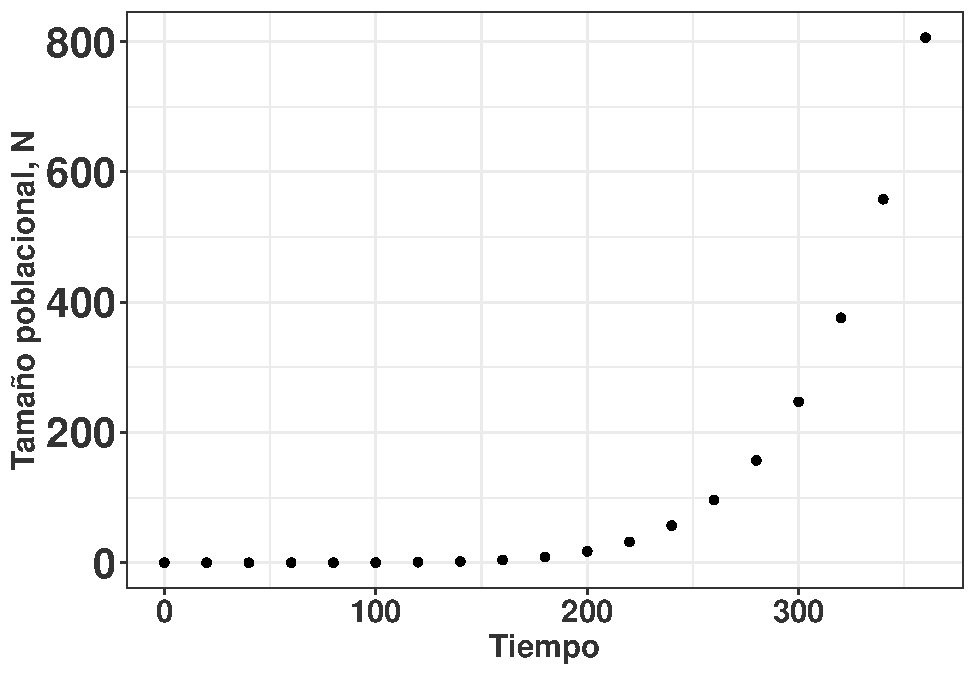
\includegraphics{Diagnostico_Poblacional_files/figure-latex/Pop-fig_1-1.pdf}
\caption{(\#fig:Pop-fig\_1)Cambio poblacional en tiempo}
\end{figure}

\section{El analisis de Dinámica Poblacional y su uso}\label{el-analisis-de-dinuxe1mica-poblacional-y-su-uso}

Determinar el tamaño poblacional en el futuro tiene muchos usos. Se puede dividir sus usos en tres grupos grandes, entender las \textbf{1)} interacciones ecológicas, \textbf{2)} manejo y conservaciones o \textbf{3)} los procesos evolutivos. Los estudios enfocado a la conservación se engloba dentro de un acercamiento de la viabilidad de poblaciones. En este libro estaremos dando una introducción a cada uno de estas vertientes, pero nuestros ejemplos son una introducción al tema y no una profundización extensa de cada uno. En la table \ref{USO} vemos algunos de los usos específicos que se ha dado con la metodología de MPP. La lista de como se ha usado los análisis de PPM proviene en parte de las ideas de Morris and Doak \citep{morris2002quantitative} y expandido.

\subsection{Tabla: El uso potencial de la diferentes acercamiento de PPM.}\label{USO}

NOTA IMPORTANTE: \emph{Evaluar las referencias y añadir referencias tradicionales y recientes}

\begin{longtable}[]{@{}
  >{\raggedright\arraybackslash}p{(\columnwidth - 6\tabcolsep) * \real{0.2297}}
  >{\raggedright\arraybackslash}p{(\columnwidth - 6\tabcolsep) * \real{0.2703}}
  >{\raggedright\arraybackslash}p{(\columnwidth - 6\tabcolsep) * \real{0.2297}}
  >{\raggedleft\arraybackslash}p{(\columnwidth - 6\tabcolsep) * \real{0.2703}}@{}}
\toprule\noalign{}
\begin{minipage}[b]{\linewidth}\raggedright
Categoria de Uso
\end{minipage} & \begin{minipage}[b]{\linewidth}\raggedright
Uso especifico
\end{minipage} & \begin{minipage}[b]{\linewidth}\raggedright
Referencias generales
\end{minipage} & \begin{minipage}[b]{\linewidth}\raggedleft
Referencias con Oquideas
\end{minipage} \\
\midrule\noalign{}
\endhead
\bottomrule\noalign{}
\endlastfoot
Manejo & Identificar las etapas o procesos demográficos claves & \citep{crouse1987stage} & ? \\
& Determinar cuantos individuos en una población es necesario para reducir la extinción & \citep{shaffer1981minimum, armbruster1993population} & ? \\
& Determinar cuantos individuos se necesita introducir en una sitio para establecer una población viable & \citep{bustamante1996population} & ? \\
& Determinar cuantos individuos se puede extraer si tener un impacto negativo sobre la viabilidad de una población & \citep{nantel1996population} & ? \\
& En especies invasivas determinar cuantos y cual etapas se necesita remover para controlar la población & \citep{arroyo2022prescriptions} & ? \\
& Determinar cuantas poblaciones se necesita para la viabilidad de una especie al nivel local o global & \citep{lindenmayer1996ranking} & \\
Evaluación de riesgos & Evaluar el riesgo de una población & \citep{gotelli2006forecasting} & muchos \\
& Comparando el riesgo relativo de dos o más poblaciones & \citep{earl2019evaluating} & ? \\
Interacciones ecologicas & Evaluar interacciones ecológicas para entender las variables importantes para la supervivencia de una población & \citep{halpern2006approaches} & Ospina et al., 2022 \\
Procesos y patrones evolutivos & Cual de los procesos y patrones evolutivos del ciclo de vida de especies impacta su crecimiento & \citep{coste2020analysis} & ? \\
\end{longtable}

\subsection{USO 1: Identificar las etapas or procesos demográficos claves}\label{uso-1-identificar-las-etapas-or-procesos-demogruxe1ficos-claves}

Identificar y conocer cuales son las etapas de vida más susceptibles y relacionados a cambios abióticos y bióticos. Aclarar cuales de las etapas/edades son más susceptibles y que resulta en cambios demográficos y su impacto sobre la persistencia de una población es necesario para el manejo. El ejemplo clásico en la literatura usando PPM son los trabajos sobre la dinámica poblacional de la tortuga ``boba'' o ``cabezona'' \emph{Caretta caretta} \citep{crouse1987stage}, \citep{crowder1994predicting}. Crouse y Crowder demostraron que aun salvando TODOS los huevos de depredación, esa estrategia de manejo antropogénico iba a tener muy poco impacto en el crecimiento de la población. Lo que encontraron es que el impacto más grande sobre el crecimiento poblacional provendría de proteger los adultos y reducir la mortandad de los adultos específicamente a causa de la mortandad de los adultos en las redes de pesca. Modificando estas redes para que las tortugas se pueden escapar y no ahogarse en las redes tendría un impacto más grande que salvar un huevos. Los trabajos de Crouse y Crowder \citep{crouse1987stage}, \citep{crowder1994predicting} fueron pioneros en demostrar que uno podía simular diferentes escenarios basado en la historia de vida y evaluar su impacto. Naturalmente, eso no quiso decir que no se debería proteger los huevos, pero que el impacto de proteger los huevos era menor que proteger los adultos.

Ejemplo de orquidea AQUI

\subsection{USO 2: Determinar cuantos individuos en una población es necesario para reducir la extinción}\label{uso-2-determinar-cuantos-individuos-en-una-poblaciuxf3n-es-necesario-para-reducir-la-extinciuxf3n}

El efecto de tamaño poblacional sobre la biología y la probabilidad de extinción es bien conocido \citep{shaffer1985population, nunney1993assessing, harris2022abundance}. ¿Cual es la probabilidad de extinción de una población considerando la cantidad de individuos en cada etapa? En general lo que se observa es que menor el tamaño poblacional, \emph{N}, mayor es el riesgo de extinción. Esa correlación de extinción con el tamaño de muestra puede variar si algunas etapas del ciclo de vida es muy reducido o su probabilidad de sobrevivir es baja o la probabilidad de crecer a la próxima etapa varia. En orquídeas es probable que una de las etapas más vulnerable es la etapa de semilla. Consideramos por ejemplo cual es la probabilidad de que las semillas se establece, germina y crezca hasta ser un juvenil en el medio ambiente. Cada una de esas probabilidades de transiciones son muy pequeñas. Por consecuencia establecer una nueva población de orquídea necesita considerar la cantidad de individuos que este presente pero también la probabilidad de tener semillas y que estás pueden crecer a ser adultos que se pueden reproducir. Sin duda la orquídeas tienen un potencial enorme de crecer. Darwin \citep{darwin1877various} estimó que un fruto de \emph{Orchis maculata} produce 6,200 semillas y una planta pudiese tener 30 capsula produciendo 186,300 semillas y en un acre la suma de las plantas produce más de 32,400,000,000 semillas!!!! Sin duda la probabilidad de que una semilla germina y produce una planta es muy pequeña sino estaríamos cubierto de orquídea en dos generaciones.

\subsection{USO 3: Determinar cuantos individuos se necesita introducir en una sitio para establecer una población viable}\label{uso-3-determinar-cuantos-individuos-se-necesita-introducir-en-una-sitio-para-establecer-una-poblaciuxf3n-viable}

Naturalmente, más cantidad de individuos re-introducido en un sitio mayor sera la probabilidad que la población sea viable, asumiendo que los individuos fueron establecidos en un area donde todas las etapas pueden sobrevivir, crecer y reproducirse. Pero, como todo, hay un limite de tiempo y esfuerzo disponible. Por consecuencia la pregunta debería ser orientado a determinar cual es el mínimo de individuos que se debería introducir para garantizar un \textbf{x} porciento de suceso en el establecimiento de una nueva población.

En los últimos años, muchas organizaciones y científicos han comenzado a hacer re-introducción de especies en su hábitat nativo y no. (ref) incluyendo algunos programa introduce especies en áreas urbanas.

En Corea dos trabajos demuestra que la re-introducción de orquídeas en un sitio puede ser parcialmente exitoso. Los autores translocarón la orquídea \emph{Thrixspermum japonicum} en la isla de Jeju donde la cantidad de individuos pre-localización era cerca de 50 y solamente un individuo produjo frutos, de allí propagaron plántulas y fueron translocado en la isla. de los 216 individuos 73\% sobrevivieron el primer año y 63\% el segundo año. De estos individuos el porcentaje de individuos que produjeron frutos fue de 16\% a 35\% en los dos años \citep{kim2016restoration}. En otro estudio en Corea, En un trabajo masivo de re-introducción de la orquídea \emph{Dendrobium moniliforme} en la isla de Bogildo, Corea, más de 13,000 individuos artificialmente propagado fueron en su ambiente natural y seguido por múltiples años. Demostraron que el sitio de localización es una variable importante para el crecimientos de los individuos. Las áreas abiertas con luz solar directa tuvieron un crecimiento más rápido que las áreas con sombra y que la especie de árbol tiene una impacto significativo en el crecimiento \citep{kim2016restoration}.

Lawrence Zettler

AQUI poner ejemplos de trabajos usando PPM para establecer N para la re-nintroduccion

\begin{itemize}
\item
  Caladenia
\item
  one million orchids project: Escribi a Fairchild para ver si tienen datos.
\item
  ????
\end{itemize}

Desafortunadamente ninguno de los trabajos mencionado arriba de Orquídeas toma ventaja de los métodos de PPM para evaluar el tamaño de re-introducción sobre el impacto de la supervivencia de orquídeas en un sitio y cuantos individuos se debería relocalizar en su ambiente natural para establecer una población viable. En general, la re-introducción de orquídeas es un tema que necesita más investigaciones y evaluaciones.

\subsection{USO 4: Determinar cuantos individuos se puede extraer sin tener un impacto negativo sobre la viabilidad de una población}\label{uso-4-determinar-cuantos-individuos-se-puede-extraer-sin-tener-un-impacto-negativo-sobre-la-viabilidad-de-una-poblaciuxf3n}

Hay tres razones principales para la extracción de individuos de su ambiente natural.

\begin{enumerate}
\def\labelenumi{\arabic{enumi}.}
\tightlist
\item
  Obtener individuos para la conservación \emph{Ex Situ}.
\item
  Usar un grupo de individuos para su propagación.
\item
  Extracción para la venta sin objetivo de conservación.
\end{enumerate}

El supuesto de colectores de orquídea de su hábitat naturales, tanto para la conservación de \emph{Ex situ} y el uso para la propagación es que el impacto es mínimo, y no tendrá impacto a largo plazo para la supervivencia. Regresaremos sobre este punto más tarde. La historia de fanatismo de recolección de orquídeas para la venta es bien conocida ref(). Aun que uno quisiera pensar que estas extracciones son del pasado y no ocurren hoy en día, hay todavía escrúpulos que extraen los plantas sin pensar al impacto que tendrá sobre la población o especie.

Pero la pregunta se tiene que hacer. Cuantos individuos y de que etapas se puede extraer de la población sin tener impacto en el crecimiento poblacional?

\subsection{USO 5: En especies invasivas determinar cuantos y cual etapas se necesita remover para controlar la población.}\label{uso-5-en-especies-invasivas-determinar-cuantos-y-cual-etapas-se-necesita-remover-para-controlar-la-poblaciuxf3n.}

Ahora es común reconocer el impacto negativo que puede tener organismos invasivos sobre la flora y la fauna local. Cual son las características que hace que una especie puede ser invasiva y cual características si fuese manejada pudiese reducir su impacto. En general, las especies invasivas tienen una tasa de crecimiento alta, una tasa de reproducción alta, una tasa de supervivencia alta y una tasa de dispersión alta. Por consecuencia, una estrategia de manejo debería considerar cual de estas etapas es más susceptible a ser manejado. En general, la etapa de semilla es la más susceptible a ser manejado. Algunos de los impacto de especies invasivas son de Australia y son bien conocidos y discutidos en clases de ecología, tal como la introducción del conejo, \emph{Oryctolagus cuniculus} \citep{alves2022single}, del cactus \emph{Opuntia} \citep{novoa2015introduced} entre muchos otros. En general, la introducción de especies invasivas es un tema que necesita más investigaciones y evaluaciones.

Algunos ejemplos de estudios usando PPM para evaluar la demografía de especies invasivas incluye \citep{koop2005projection, mcmahon2008transient, li2015demographic}.

Falta ejemplos de orquídeas FALCON et al.~

\subsection{USO 6: Evaluar el riesgo de una población}\label{uso-6-evaluar-el-riesgo-de-una-poblaciuxf3n}

La gran mayoría de los estudios realizados usando PPM es para evaluar el riesgo de reducción poblacional o el riesgo de extinción. Un trabajo ejemplar es el de Forsman \citep{forsman1996demography} donde evaluó 11 poblaciones del ``spotted owl'' donde demostró que 10 de estas poblaciones estaban en declive y que la población de California estaba en riesgo de extinción. Análisis usando PPM como herramienta para evaluar el riesgo de extinción incluye estimados distintos, como el riesgo de extinción, el cuasi-extinción y la probabilidad de cuasi-extinción y naturalmente son utilizado para especies donde se quiere hacer un manejo de la demografía de esta para reducir el riesgo de extinción \citep{crone2011plant, semmens2016quasi}. El uso de este acercamiento aun que es común en la literatura de conservación pudiese ser problemático si no se considera la confiabilidad de los parámetros estimados y la incertidumbre de los datos \citep{ludwig1999meaningful}.

Falta ejemplos de orquídeas

\subsection{USO 7: Determinar cuantas poblaciones se necesita para la viabilidad de una especie al nivel local o global}\label{uso-7-determinar-cuantas-poblaciones-se-necesita-para-la-viabilidad-de-una-especie-al-nivel-local-o-global}

\ldots\ldots{} Sobre metodos de PPM

Un otro método de evaluar el riesgo de múltiples poblaciones es por estudiar la dinámica de metapoblaciones (se define como poblaciones de poblaciones) y es un acercamiento más sencillo para evaluar la dinámica de poblaciones, pero en la mayoría de los casos no se recolecta información sobre la estructura de edades o etapas de los individuos, pero el cambio en numero de individuos, la colonización y extinción de sitios previamente ocupado para evaluar la persistencia del conjunto de las poblaciones. Ese acercamiento es muy útil para evaluar la viabilidad de una especie en un conjunto de sitios. Pero la lista de estudios de metapoblaciones es limitada a unos artículos \citep{tremblay2006epiphytic, lind2007metapopulation, winkler2009population, kindlmann2014disobedient, acevedo2015spatial, acevedo2020local, vsvecova2023difficulties}. Para una introducción a los conceptos y métodos de análisis vea el libro de Hanski \citep{hanski1999metapopulation}.

\subsection{USO 8: Comparando el riesgo relativo de dos o más poblaciones}\label{uso-8-comparando-el-riesgo-relativo-de-dos-o-muxe1s-poblaciones}

\subsection{USO 9: Evaluar interacciones ecológicas para entender las variables importantes para la supervivencia de una población}\label{uso-9-evaluar-interacciones-ecoluxf3gicas-para-entender-las-variables-importantes-para-la-supervivencia-de-una-poblaciuxf3n}

\subsection{USO 10: Cual de los procesos y patrones evolutivos del ciclo de vida de especies impacta su crecimiento}\label{uso-10-cual-de-los-procesos-y-patrones-evolutivos-del-ciclo-de-vida-de-especies-impacta-su-crecimiento}

\section{Historia de dinamica poblacional en orquideas.}\label{historia-de-dinamica-poblacional-en-orquideas.}

\section{Referencias}\label{referencias}

\chapter{Qué es un diagrama de Ciclo de Vida}\label{quuxe9-es-un-diagrama-de-ciclo-de-vida}

Por: Nhora Ospina

\section{Ejemplos de ciclos de Vida}\label{ejemplos-de-ciclos-de-vida}

Escribo algo

\section{Ejemplos de un ciclo de vida sencillo}\label{ejemplos-de-un-ciclo-de-vida-sencillo}

Tengo mucho texto que ampliar

\section{Ejemplo de un ciclo de vida con 3 estadios}\label{ejemplo-de-un-ciclo-de-vida-con-3-estadios}

\begin{Shaded}
\begin{Highlighting}[]
\FunctionTok{library}\NormalTok{(Rage)}
\end{Highlighting}
\end{Shaded}

\begin{Shaded}
\begin{Highlighting}[]
\CommentTok{\# hidden code to produce figures}
\FunctionTok{library}\NormalTok{(DiagrammeR)}
\NormalTok{matA }\OtherTok{\textless{}{-}} \FunctionTok{rbind}\NormalTok{(}
  \FunctionTok{c}\NormalTok{(}\FloatTok{0.0}\NormalTok{, }\FloatTok{0.0}\NormalTok{, }\FloatTok{3.2}\NormalTok{),}
  \FunctionTok{c}\NormalTok{(}\FloatTok{0.5}\NormalTok{, }\FloatTok{0.3}\NormalTok{, }\FloatTok{0.8}\NormalTok{),}
  \FunctionTok{c}\NormalTok{(}\FloatTok{0.0}\NormalTok{, }\FloatTok{0.4}\NormalTok{, }\FloatTok{0.9}\NormalTok{)}
\NormalTok{)}


\NormalTok{stages }\OtherTok{\textless{}{-}} \FunctionTok{c}\NormalTok{(}\StringTok{"semillas"}\NormalTok{, }\StringTok{"plantulas"}\NormalTok{, }\StringTok{"adultos"}\NormalTok{)}
\NormalTok{title }\OtherTok{\textless{}{-}} \ConstantTok{NULL}
\NormalTok{graph }\OtherTok{\textless{}{-}} \FunctionTok{expand.grid}\NormalTok{(}\AttributeTok{to =}\NormalTok{ stages, }\AttributeTok{from =}\NormalTok{ stages)}
\NormalTok{graph}\SpecialCharTok{$}\NormalTok{trans }\OtherTok{\textless{}{-}} \FunctionTok{round}\NormalTok{(}\FunctionTok{c}\NormalTok{(matA), }\DecValTok{3}\NormalTok{)}
\NormalTok{graph }\OtherTok{\textless{}{-}}\NormalTok{ graph[graph}\SpecialCharTok{$}\NormalTok{trans }\SpecialCharTok{\textgreater{}} \DecValTok{0}\NormalTok{, ]}
\NormalTok{nodes }\OtherTok{\textless{}{-}} \FunctionTok{paste}\NormalTok{(}\FunctionTok{paste0}\NormalTok{(}\StringTok{"\textquotesingle{}"}\NormalTok{, stages, }\StringTok{"\textquotesingle{}"}\NormalTok{), }\AttributeTok{collapse =} \StringTok{"; "}\NormalTok{)}
\NormalTok{graph}\SpecialCharTok{$}\NormalTok{min\_len }\OtherTok{\textless{}{-}}\NormalTok{ (}\FunctionTok{as.numeric}\NormalTok{(graph}\SpecialCharTok{$}\NormalTok{to) }\SpecialCharTok{{-}} \FunctionTok{as.numeric}\NormalTok{(graph}\SpecialCharTok{$}\NormalTok{from)) }\SpecialCharTok{*} \DecValTok{3}
\NormalTok{graph}\SpecialCharTok{$}\NormalTok{col }\OtherTok{\textless{}{-}} \FunctionTok{c}\NormalTok{(}
  \StringTok{"PaleGreen4"}\NormalTok{, }\StringTok{"PaleGreen4"}\NormalTok{, }\StringTok{"PaleGreen4"}\NormalTok{, }\StringTok{"Goldenrod1"}\NormalTok{,}
  \StringTok{"MediumOrchid4"}\NormalTok{, }\StringTok{"PaleGreen4"}
\NormalTok{)}
\NormalTok{edges }\OtherTok{\textless{}{-}} \FunctionTok{paste0}\NormalTok{(}\StringTok{"\textquotesingle{}"}\NormalTok{, graph}\SpecialCharTok{$}\NormalTok{from, }\StringTok{"\textquotesingle{}"}\NormalTok{, }\StringTok{" {-}\textgreater{} "}\NormalTok{, }\StringTok{"\textquotesingle{}"}\NormalTok{, graph}\SpecialCharTok{$}\NormalTok{to, }\StringTok{"\textquotesingle{}"}\NormalTok{,}
  \StringTok{"[minlen="}\NormalTok{, graph}\SpecialCharTok{$}\NormalTok{min\_len,}
  \StringTok{",fontsize="}\NormalTok{, }\DecValTok{10}\NormalTok{,}
  \StringTok{",color="}\NormalTok{, graph}\SpecialCharTok{$}\NormalTok{col,}
  \StringTok{",xlabel="}\NormalTok{, }\FunctionTok{paste}\NormalTok{(}\StringTok{"}\SpecialCharTok{\textbackslash{}"}\StringTok{"}\NormalTok{, graph}\SpecialCharTok{$}\NormalTok{trans),}
  \StringTok{"}\SpecialCharTok{\textbackslash{}"}\StringTok{]}\SpecialCharTok{\textbackslash{}n}\StringTok{"}\NormalTok{,}
  \AttributeTok{collapse =} \StringTok{""}
\NormalTok{)}
\FunctionTok{grViz}\NormalTok{(}
  \FunctionTok{paste}\NormalTok{(}
    \StringTok{"}
\StringTok{digraph \{}
\StringTok{  \{}
\StringTok{    graph[overlap=false];}
\StringTok{    rank=same;}
\StringTok{    node [shape="}\NormalTok{, }\StringTok{"egg"}\NormalTok{, }\StringTok{", fontsize="}\NormalTok{, }\DecValTok{12}\NormalTok{, }\StringTok{"];"}\NormalTok{,}
\NormalTok{    nodes, }\StringTok{"}
\StringTok{  \}"}\NormalTok{,}
    \StringTok{"ordering=out}
\StringTok{  x [style=invis]}
\StringTok{  x {-}\textgreater{} \{"}\NormalTok{, nodes, }\StringTok{"\} [style=invis]"}\NormalTok{, edges,}
    \StringTok{"labelloc=}\SpecialCharTok{\textbackslash{}"}\StringTok{t}\SpecialCharTok{\textbackslash{}"}\StringTok{;}
\StringTok{  label=}\SpecialCharTok{\textbackslash{}"}\StringTok{"}\NormalTok{, title, }\StringTok{"}\SpecialCharTok{\textbackslash{}"}
\StringTok{\}"}
\NormalTok{  )}
\NormalTok{) }
\end{Highlighting}
\end{Shaded}

\begin{verbatim}
## PhantomJS not found. You can install it with webshot::install_phantomjs(). If it is installed, please make sure the phantomjs executable can be found via the PATH variable.
\end{verbatim}

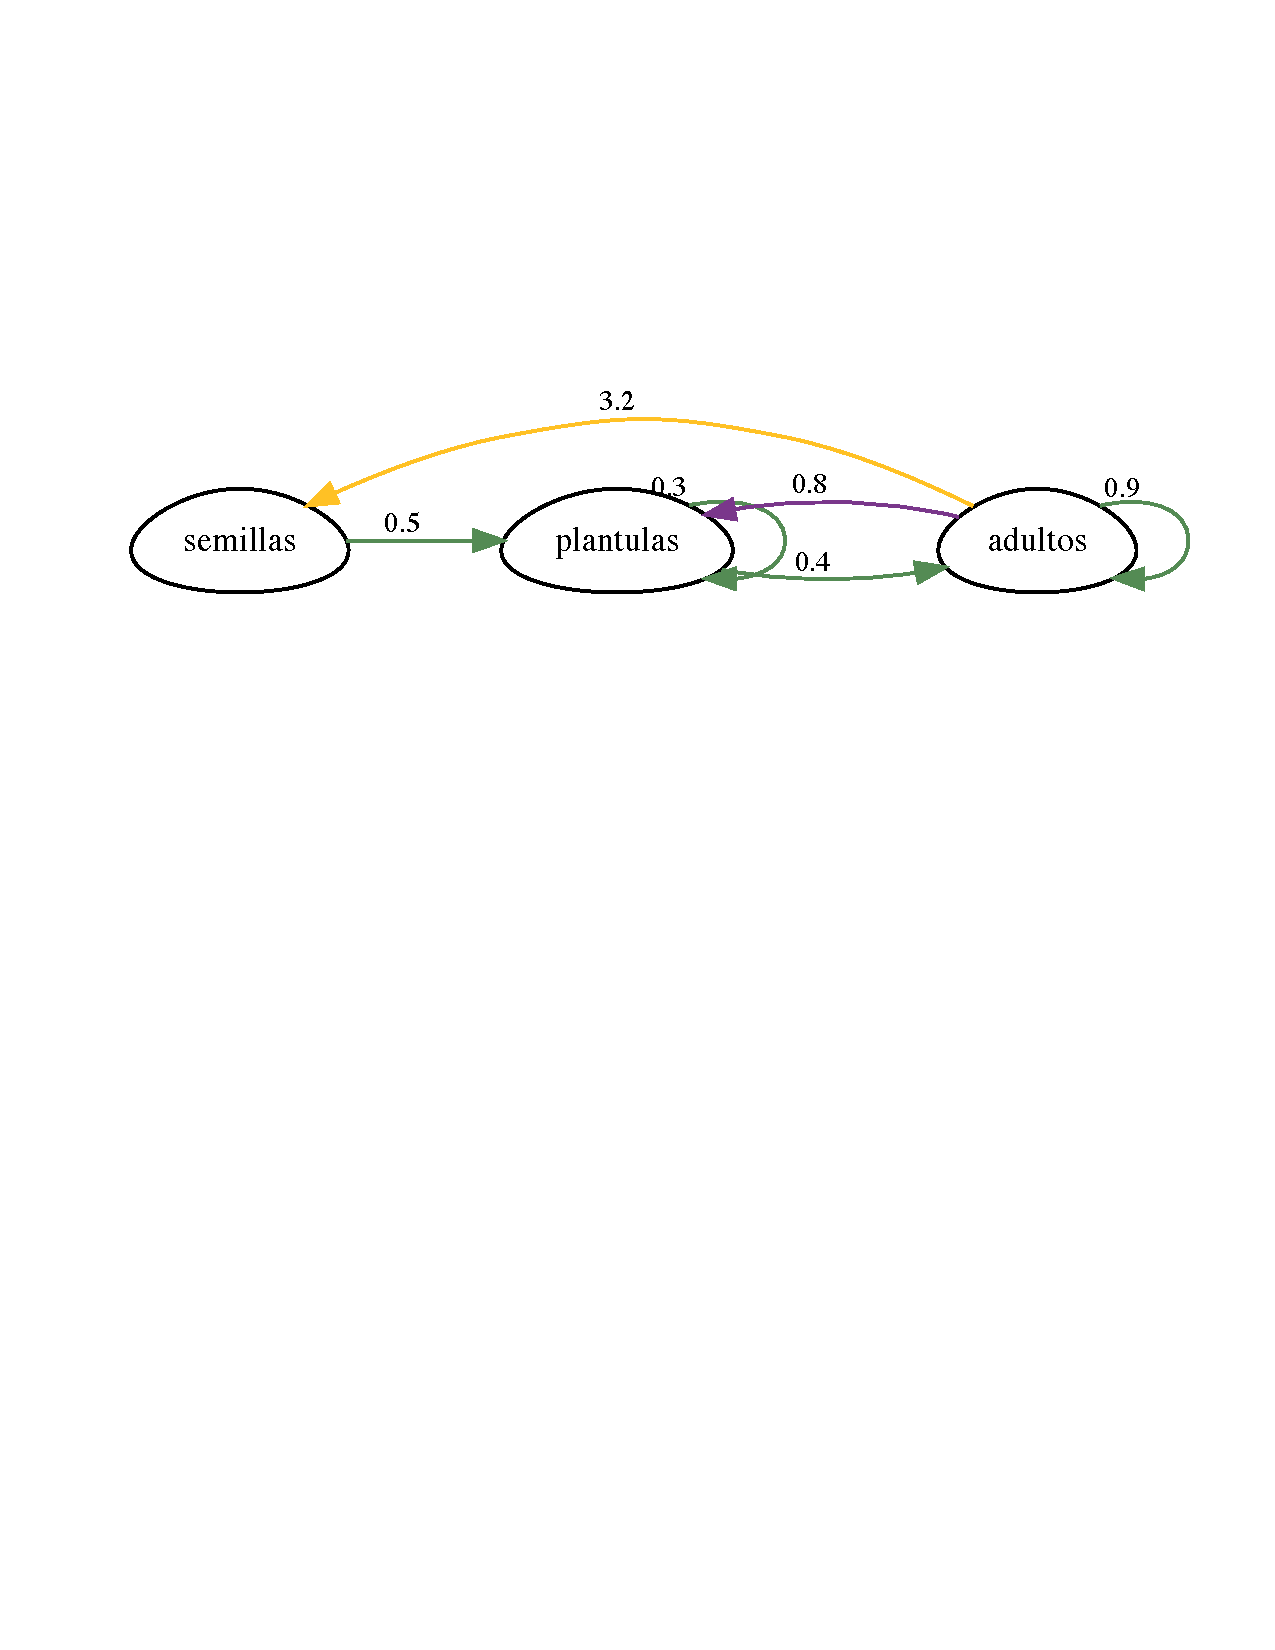
\includegraphics{Diagnostico_Poblacional_files/figure-latex/chap2_2-1.pdf}

\section{Ejemplo de un cicle de vida con estadio de latencia}\label{ejemplo-de-un-cicle-de-vida-con-estadio-de-latencia}

\begin{Shaded}
\begin{Highlighting}[]
\FunctionTok{library}\NormalTok{(ggplot2)}
\FunctionTok{plot\_life\_cycle}\NormalTok{(matA, }\AttributeTok{stages=}\NormalTok{stages, }\AttributeTok{fontsize =} \DecValTok{0}\NormalTok{)}
\end{Highlighting}
\end{Shaded}

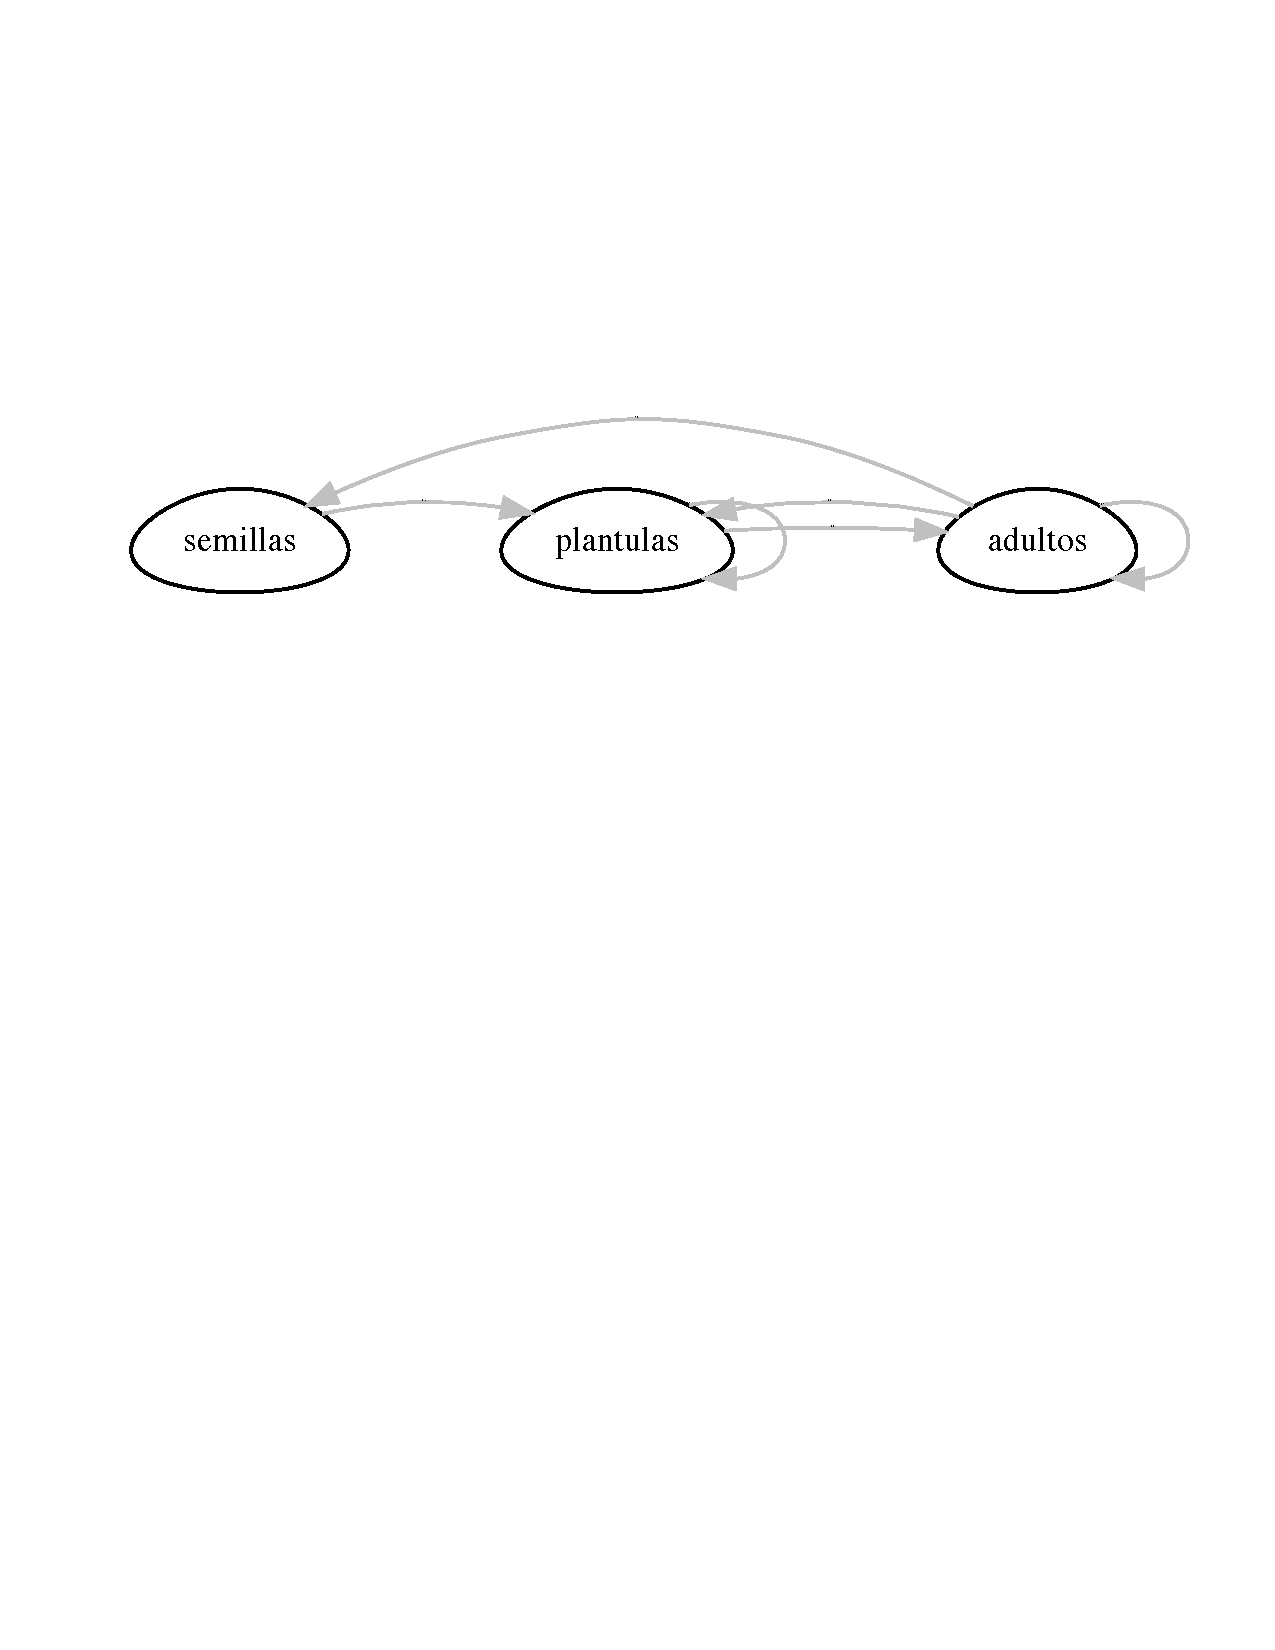
\includegraphics{Diagnostico_Poblacional_files/figure-latex/chap2_3-1.pdf}

\section{Code for color coding figure}\label{code-for-color-coding-figure}

\url{http://rich-iannone.github.io/DiagrammeR/}

\section{Ejemplo de un cicle de vida con estadio de post reproducción}\label{ejemplo-de-un-cicle-de-vida-con-estadio-de-post-reproducciuxf3n}

\section{Ejemplo de un cicle de vida incompleto (y biologicamente erroneos)}\label{ejemplo-de-un-cicle-de-vida-incompleto-y-biologicamente-erroneos}

\section{Referencias}\label{referencias-1}

\chapter{Como recopilar datos en el campo}\label{como-recopilar-datos-en-el-campo}

\section{Consideraciones en la colecta de datos en el campo}\label{consideraciones-en-la-colecta-de-datos-en-el-campo}

Por: Aucencia Emeterio-Lara, Mariana Hernández-Apolinar y Raymond L. Tremblay

\section{Tipo de crecimiento en las orquídeas}\label{tipo-de-crecimiento-en-las-orquuxeddeas}

Conocer el tipo de crecimiento y la apariencia general de la planta de interés es un primer paso en la toma de datos en el campo, ya que a partir de esto sabremos dónde ubicarlas y cómo identificarlas las etapas con facilidad en su medio natural.
Es así que hay que identificar el sustrato en el que se establecen las orquídeas (i.e.~tipo de crecimiento), mismo que puede ser terrestre, epífito o rupícola, éste último también llamado litófito \citep{tellez2007orquideas}.
Como es evidente, en el primer caso las plantas se desarrollan en suelo, en el segundo sobre ramas y troncos los árboles, mientras que en el tercero grupo sobre rocas.
Es importante reconocer que algunas especies no son estrictamente limitado a un tipo de ambiente, por ejemplo hay algunas especies de \emph{Lepanthes} que son epífita y rupícula.

De acuerdo con sus rasgos morfológicos o apariencia se pueden identificar al menos tres grupos de orquídeas epífitas: plantas con tallos engrosados y modificados conocidos como pseudobulbos (e.g \emph{Laelia}, \emph{Oncidium}, \emph{Encyclia}, \emph{Stanhopea}, \emph{Maxilaria}, \emph{Rhynchostelle}, etc), plantas con tallos simples o delgados (e.g \emph{Epidendrum}, \emph{Dichea}) y un tercer grupo con hojas engrosadas y tallos compactos o pseudobulbos poco visibles (e. g. \emph{Trichocentrum}).
En el caso de las orquídeas terrestres se pueden identificar seis grupos: plantas con tallos y hojas alternas o en espiral (v. g. \emph{Cypripedium}, \emph{Dichromanthus}, \emph{Habenaria}, \emph{Triphora}), plantas con hojas solitarias o en pares (v.g. \emph{Bletia}, \emph{Schiedeella}, \emph{Malaxis}, \emph{Govenia}), plantas con hojas en roseta (\emph{Brachystele}, \emph{Deiregyne}, \emph{Sarcoglottis}), plantas con hojas en abanico (\emph{Paphiopedilum}, \emph{Phragmipedium}), plantas sin hojas (\emph{Rhizanthella}, \emph{Triphora}) y plantas con pseudobulbos (\emph{Oeceoclades}, \emph{Cymbidium}).
Por su parte, en las plantas rupícolas se identifica un dos grupos: plantas con pseudobulbos (\emph{Cattleya}, \emph{Hoffmannsegella}, \emph{Laelia}, \emph{Paphiopedillum}) o sin pseudobulbo (\emph{Lepanthes}).
Cabe señalar que, si bien esta clasificación es de utilidad y brinda una idea de la diversidad en la morfología vegetativa de las orquídeas, hay que considerar que solo se basa en su apariencia, por lo que es muy cualitativa y poco rigurosa desde el punto de vista botánico.

\section{Métodos y técnicas de muestreo}\label{muxe9todos-y-tuxe9cnicas-de-muestreo}

El método y técnica de muestreo depende en gran medida del tipo de crecimiento (i.e.~epífito, rupícola o terrestre) que presente la especie de interés.
No solo eso, también de esta condición depende el grado de dificultad y el tiempo que se invertirá en la toma de datos.
Para facilitar esta colecta de información se han implementado distintas técnicas de muestreo según su tipo de crecimiento, las cuales se describen a continuación.

\subsection{\texorpdfstring{\emph{Orquídeas epífitas y rupícolas}.}{Orquídeas epífitas y rupícolas.}}\label{orquuxeddeas-epuxedfitas-y-rupuxedcolas.}

Las orquídeas epífitas y rupícolas viven a distintas alturas en árboles y acantilados.
En la colecta de información de estas poblaciones se utilizan desde una simple escalera hasta equipo de alpinismo para ascenso.
El uso de escaleras es una técnica muy práctica si la especie de estudio se desarrolla en las zonas bajas de los acantilados o en forofítos como arbustos y árboles de porte bajo a medio \citep{hernandez1992dinamica} ; sin embargo, se tiene la desventaja de transportar este instrumento de trabajo hasta el sitio de muestreo.

Cuando las orquídeas se distribuyen a una altura considerable del acantilado, la técnica de rapel resulta muy útil y segura e implica el descenso mediante cuerdas hasta llegar a las orquídeas a muestrear.
Por su parte, la técnica de ascenso de una sola cuerda es muy segura \citep{jepson2000tree} cuando se trata de orquídeas epífitas habitando hospederos de porte medio y alto con troncos y ramas gruesas.
Pero tiene algunas limitaciones como es la dificultad de acceder a ramas delgadas en los estratos muy altos.
En importante señalar que, si se carece de experiencia en el ascenso de árboles y acantilados es importante recibir apoyo de gente experta.

En el muestreo de los árboles se señala la ubicación preferente de las orquídeas de estudio, debido a que éstas presentan condiciones microclimáticas variables.
Dicha ubicación, generalmente toma en cuenta la clasificación hecha por Johansson \citep{johansson1974ecology, catling1986epiphytic}, quien señala que en un árbol hospedero existen cinco zonas o estratos, dividiéndolos de la siguiente manera: la parte basal del tronco (Zona I), tronco principal (Zona II), la copa interna (Zona III), la copa media (Zona IV) y la copa externa (Zona V).
Cabe señalar que, la mayor concentración de orquídeas epífitas se registra en los estratos medios II, III, IV \citep{mondragon2007life}.

\textbf{AQUI un dibujo del concepto sugerido por Johansson (1974) y Cattling (Quien puede hacer un dibujo que se acerca al concepto sugerido por el y Cattling? NO deberiamos usar una foto de otro papers, habria que pedir permiso.}

\subsection{\texorpdfstring{\emph{Orquídeas terrestres}.}{Orquídeas terrestres.}}\label{orquuxeddeas-terrestres.}

En el muestreo de poblaciones de orquídeas terrestres se han implementado varias técnicas de muestreo, en esta sección nos referiremos a dos: El método de triangulación y el método sin área.
El primero permite estimar el área en que se establece la población, mientras que el segundo no permite establecer esta variable y se centra en el marcaje de individuos.
A continuación se detalla en qué consisten ambos.

\begin{enumerate}
\def\labelenumi{\alph{enumi})}
\tightlist
\item
  \emph{Método de triangulación}. El método de triangulación es una técnica no invasiva y comúnmente es utilizada para monitorear las poblaciones terrestres en Australia \citep{tremblay2009population}. El método consiste en clavar dos estacas o clavijas permanentes en el suelo. La distancia entre la primeera estaca y segunda estaca generalmente es de un metro. Sobre las estacas se puede: 1) sobreponer un cuadro de madera o tubos de PVC, cuyos lados están divididos en centímetros o 2) colocar cintas métricas sobre cada uno de los lados del cuadrado hecho. Estas dos variantes del método se utilizan para ubicar a los individuos dentro del cuadro al indicarse la distancia de la planta respecto a dos de los lados (un sistema \textbf{x} e \textbf{y}). Esta técnica es muy buena cuando los individuos están separados uno del otro, pero hay que tener cuidado cuando están muy cercanos (menos de 1 cm de distancia). Además, es fácil de implementarse, es muy precisa y deja muy poca evidencia en el campo.
\end{enumerate}

\begin{figure}
\centering
\includegraphics[width=1\textwidth,height=4.16667in]{Figures/Triangulation_Method.pdf}
\caption{Métodos de triangulación para muestreo: los P\_x representa la posición de cada planta. Dos distancia son medidas, cada una de la estaca. Nota que este método no se añade un identificador individual a las plantas.}
\end{figure}

\begin{enumerate}
\def\labelenumi{\alph{enumi})}
\setcounter{enumi}{1}
\tightlist
\item
  \emph{Método de sin área}. En campo, las orquídeas terrestres forman pequeñas colonias, algunas de menos de 20 individuos e incluso hay especies con individuos aislados (Ej. \emph{Govenia lagenophora}, \emph{Dichromanthus cinnabarinus} y \emph{D. aurantiacus} \citep{tellez2007orquideas}, por lo que su dinámica poblacional generalmente es descrita a partir de la información obtenida en varias colonias o subpoblaciones. El método sin área ha sido ampliamente usado en este tipo de orquídeas, no es invasivo y consiste en la selección de una colonia o subpoblación en la que se marcan todas las plantas observadas en el lugar \citep{martinez2024estimation}. Asimismo, la ubicación del sitio y los individuos puede geo-referirse y/o hacer mapas de localización.
\end{enumerate}

\section{Marcaje y monitoreo de los individuos en el tiempo}\label{marcaje-y-monitoreo-de-los-individuos-en-el-tiempo}

La dinámica o cambio en una población se evalúa marcando y siguiendo a todos los individuos que se encuentran en un sitio (i.e.~censo) o de solo una parte de éstos (i.e.~muestreo) a lo largo de sus distintas etapas del ciclo de vida.
Sin importar si censamos o muestreamos, tenemos que asegurar dos aspectos durante el marcaje o etiquetado de una población:

\begin{enumerate}
\def\labelenumi{\arabic{enumi})}
\item
  que se incluyan individuos de todas las categorías de etapas/estados que conforman una población y
\item
  que el número de individuos de cada estapas/estados sea suficiente para poder llevar a cabo un análisis demográfico robusto que refleje, con cierta precisión, la dinámica de la población seleccionada.
\item
  además de esto, también debemos lograr que el registro de la información en campo sea fácil, consistente y sin error o sea minimizar los errores.
\end{enumerate}

\subsection{Etapas de las orquídeas de estudio a identificar en campo}\label{etapas-de-las-orquuxeddeas-de-estudio-a-identificar-en-campo}

Identificar las etapas/estados de desarrollo de una especie es escencial para evaluar los cambios que ocurren en los individuos de una población a lo largo de su ciclo de vida.
Para cambios en las etapas de los individuos en el tiempo se debe identificar las características biológicas y morfológicas que definen cada una de las etapas/estados de desarrollo de los individuos de la población.
Esta serie de características permitirá reconocer y diferenciar las semillas, plántulas, juveniles, adultos y etapas latentes (cuando las haya); asimismo a partir de su monitoreo o seguimiento se reconocerá su cambio de etapa/estado en el tiempo.

Existen características que son distintivas de una etapa/estado en particular, tal es el caso de estructuras reproductivas (flores, frutos y escapos frescos o secos), las cuales son distintivas de los individuos adultos y permiten diferenciar estados de desarrollo en las plantas.
No obstante, cuando se trata de especies de un mismo género que comparten un mismo hábitat, es posible confundir a los individuos de diferente estapas, plantulas, juneniles y adultos de distintas especies debido a que pueden presentar características vegetativas o florales muy similares.
A pesar de esto, y con la ayuda de un botánico experimentado, es posible resolver la mayoría de estos dilemas.
Por su parte, los individuos juveniles o no reproductivos serán aquellos que no presenta flores ni frutos, y son distintos a las plántulas, que son los individuos recién establecidos.

Dos de las etapas de desarrollo más difíciles de seguir en campo son las semillas y plántulas, por lo que para su caracterización y muestreo en campo hay que considerar lo siguiente:

\subsubsection{\texorpdfstring{\emph{Semillas}.}{Semillas.}}\label{semillas.}

La fase de semillas es uno de los mayores retos en el estudio de las orquídeas, ya que sus tamaño tan pequeño (i.e.~son conocidas como semillas polvo o ``dust-seeds'') dificulta el seguimiento de su dispersión, germinación y establecimiento en campo \citep{ackerman1996seedling, ticktin2020synthesis} ; los parámetros que corresponde a la supervivencia y crecimiento de semillas son de gran utilidad al momento de estimar los valores de fecundidad o de transición en el primer estadio del ciclo de vida.
La relación entre la producción de semillas y la transición a plantulas y juveniles raramente se ha estudiando raramente en las orquideas.
Actualmente en el medio natural, el método más usado para evaluar la germinación es la introducción de bolsas pequeñas de malla de plancton (mesh plankton, 50 μm) con semillas, las cuales se colocan en el suelo o en la corteza de árboles donde se añadio semillas y se recogen en uno o distintos periodos del año para evaluar la germinación \citep{rasmussen1993seed, rasmussen2011methods, anghelescu2023asymbiotic}.

\subsubsection{\texorpdfstring{\emph{Plántulas}.}{Plántulas.}}\label{pluxe1ntulas.}

Identificar las plántulas en orquídeas también tiende a ser complicado debido a que se desconoce su morfología en la gran mayoría de las especies.
Por ejemplo, en el caso de \emph{Cypripedium irapeanum}, una orquídea terrestre, las plántulas presentan tallos muy delgados y su apariencia es semejante al pasto y varias de éstas se encuentran escondidas entre la vegetación (Hernández-Apolinar, comunicación personal).
En el caso de orquídeas epífitas, se trata de los individuos más pequeños en la población, algunos se pueden reconocer si no están cubiertas de musgo, liquen u otra tipo de planta.
Tremblay (com. pers.) ha encontrado a estas pequeñas plantas en alreredor de las plantas adultas, por lo que recomienda esta estrategia para marcar correctamente esta fase de desarrollo en orquídeas terrestres o epífitas; sin embargo, un problema potencial es lograr diferenciar correctamente las plántulas de distinta especie.
En \emph{Lepanthes}, por ejemplo, las plántulas se establecen entremezclas de difer3entes especies en el mismo forofito y carecen de caracteres distintivos por lo que es imposible distinguirlas por especie (Tremblay com. pers.); esto se logra solamente cuando se marcan y siguen cuidadosamente a etapas posteriores (juvenil o adulto).
De esta manera, el autor ha logrado distinguir entre plántulas de \emph{Lepanthes eltoroensis} y \emph{L. woodburyana}, las cuales se diferencian únicamente en la forma de crecimiento del tallo.
Al continuar el desarrollo, \emph{Lepanthes eltoroensis} tendrá un crecimiento postrado, mientras que éste será erecto en \emph{L. woodburyana}.
Si bien este método es bueno, es importante considerar que puede representar un periodo de tiempo largo y que se corre el riesgo de no saber la especie cuando las plántulas no sobreviven a la siguiente etapa o el largo del estudio no es suficiente para detemrinar a cual especies pertenece las plantulas o juveniles.

\section{Identificar la características de la especie de estudio}\label{identificar-la-caracteruxedsticas-de-la-especie-de-estudio}

Para cualquier estudio usando el acercamiento de dinámica poblacional es necesario conocer lo básico de la especie de interés y las etapas/edades que corresponde al ciclo de vida de esa misma.
Poder reconocer las diferentes etapas del ciclo de vida con exactitud es esencial, por ejemplo separar entre las semillas, plántulas, juveniles y adultos y si hay etapas latentes.
Cuando se define una etapa de vida se debería tener características morfológicas que se puede identificar en el campo con facilidad y para reducir los errores de asignaciones a otras etapas.
Por ejemplo en \emph{Lepanthes} \citep{tremblay2003population} definió un juvenil como individuo que tiene tallos con vaine Lepanthiforme \emph{lepanthiform sheath} en por lo menos una de los peciolos y que no tiene evidencia de presente o anterior de inflorescencias.
Nota que aquí la diferencia entre una plántula y un juvenil es que tenga una vaina Lepanthiformey se diferencia de los adultos con la ausencia de evidencia de inflorescencias seca y activa.

Por ejemplo en la foto que sigue tenemos un individuos que tiene dos hojas, una con inflorescencia activa y la otra hoja con inflorescencia secas, por consecuencia ese individuos es un adulto ya que tiene por los menor una inflorescencia activa (produciendo flores o el potencial de producir flores).
Nota no es que la inflorescencia tenga flores es que la inflorescencia es verde.

\begin{figure}
\centering
\includegraphics[width=0.9\textwidth,height=\textheight]{Figures/lepanthes_rupestris.jpeg}
\caption{\emph{Lepanthes rupestris} con inflorescencias seca y activa. Foto: Tremblay}
\end{figure}

\subsection{Semillas}\label{semillas}

Algunos retos en el estudio de las orquídeas es el seguimiento de las semillas y plántulas en el campo.
La dispersión de las semillas en el espacio ha sido estudiado muy poco \citep{ackerman1996seedling} debido a sus tamaños tan pequeños y dificultad de seguir en el espacio.
Los métodos de seguir las semillas en su ambiente natural incluye típicamente ponerlos en una malla y ponerlos en el suelo o la corteza de un árbol y recogerlos más tarde para ver si estas germinaron \citep{rasmussen1993seed}, \citep{whigham2006seed}.
Un patrón que parecer ser consistente en las plantas es que el crecimiento poblacional tienden a ser limitado por las semillas \citep{turnbull2000plant}.

\subsection{Identificación y etiquetado de individuos.}\label{identificaciuxf3n-y-etiquetado-de-individuos.}

Debido a la naturaleza sésil de las plantas, una vez delimitada la población resulta relativamente sencillo contar e identificar a todos los individuos seleccionados.
Sin embargo, el monitoreo y secuenciación de todos y cada uno de los procesos o eventos de desarrollo por los que transita cada uno de los individuos de año a otro año (o el periodo de tiempo de su estudio: en \emph{Lepanthes} hizo muestreo mensuales no anual \citep{tremblay2003population} sólo es posible si:

\begin{verbatim}
a) contamos con material de marcaje de calidad y 
b) si tenemos un sistema de identificación sencillo y claro. 
\end{verbatim}

Estos dos sencillos pasos evitarán mezclar la información entre individuos de una misma población o confundir la información con plantas de otras poblaciones.
Es decir, la calidad de nuestros datos dependerá, en parte, de cómo marquemos y de qué calidad sea el material que usemos para el marcaje.

\begin{enumerate}
\def\labelenumi{\alph{enumi})}
\tightlist
\item
  \emph{Qué material usar al marcar o etiquetar un individuo o sitio de muestro}.
\end{enumerate}

La calidad y sobre todo la durabilidad del material de marcaje es importante cuando hacemos un estudio poblacional, más aún cuando se trata de uno de largo plazo (múltiples años).
Si las marcas se desintegran de un año a otro, se perderá la identidad de cada planta y si no nos damos cuenta podríamos suponer dos cosas en nuestro siguiente monitoreo: 1) que el individuo murió (ya que el marcador no se encuentra) o 2) que hay un nuevo reclutamiento en la población (aparece un nuevo individuo sin marca pero es un error por la perdida del identificador).
Esto sesgaría nuestros resultados al suponer un aumento en la mortalidad o, en su defecto, un aumento en el reclutamiento.
Naturalmente, estos sesgos dependeran del número de individuos que marquemos (i.e.~tamaño de la muestra).
Por regla general se ha considerado que a menor tamaño de muestra, mayor es el impacto de estos estas asignaciones de dinamica poblacional y por consecuencia mayor es el sesgo.

Las etiquetas de aluminio resultan ser un buen material al marcar los individuos de las orquídeas de cualquier ambiente (i.e.~epífito, terrestre o rupícola).
El aluminio laminado es un material relativamente barato, muy duradero y se puede escribir sobre éste; por lo que, se garantiza la permanencia de la marca o etiqueta y la de las inscripciones que hayamos hechos sobre ésta, hay tambien marcadores previamente numerado.
Además, este tipo de etiquetas puede sujetarse a la planta o colocarse cerca de ésta con diferentes materiales; por ejemplo, hilo de pescador, cinchos de plástico, alambre galvanizado o plastificado, clavos, chinchetas (drawing pin) y grapas, entre aquellos más usados.

Un aspecto que hay que cuidar al marcar individuos es que las etiquetas se enmascaren con el ambiente; es decir, que no sean muy grandes, estén protegidas y que no sean evidentes en areas donce transitan personas no asociada a la investigación, a fin de evitar su pérdida o, incluso, el robo de plantas por gente ajena a la investigación es algo que siempre debemos tratar de minimizar.

La durabilidad del material usado es muy importante cuando existen eventos en el ciclo de vida de una especie que pueden prolongarse por varios años.
Este es el caso de algunas orquídeas terrestres que pueden no rebrotar y mantenerse en latencia vegetativa por más de un ciclo anual de forma consecutiva.
Por ejemplo, en \emph{Liparis lilifolia} puede no emerger por tres o más años continuos \citep{hutchings1987population, wells1991demographic}, mientras que en \emph{Epipactis helleborine} por cinco e, incluso, siete años \citetext{\citealp[ ]{light2006appearance}; \citealp{coates2006effects}}.
El poder tener un muestreo confiable de la secuenciación de estos eventos en un individuo en el mediano y largo plazo depende de la calidad del material usado al marcar las plantas o sea el metodo de marca y recaptura, lo cual a su vez permitirá tener estimaciones confiable o segadas del tamaño poblacional y de la supervivencia y crecimiento de los individuos.

\begin{figure}
\centering
\includegraphics[width=0.6\textwidth,height=\textheight]{Figures/Cypripedium_acaule.jpg}
\caption{\emph{Cypripedium acaule} marcado en una población cerca de North Bay, Canada; Foto: Tremblay}
\end{figure}

\begin{enumerate}
\def\labelenumi{\alph{enumi})}
\setcounter{enumi}{1}
\tightlist
\item
  \emph{Como marcar los individuos}
\end{enumerate}

\emph{Marcar los sitios de muestreos}.

Al igual que los individuos, los sitios de muestreo también se marcan a fin de facilitar su ubicación en el medio natural.
Estos pueden ser marcados, usando banderines, etiquetas grandes de aluminio o plástico, cinta de señalización (flagging tape) o pintura permanente; asimismo, también se pueden georeferir y hacer mapas de localización.
Cuando se trata de marcas de colores, se deben preferir colores poco llamativos que puedan disimularse con la vegetación circundante.
Si el sitio está bien protegido se puede optar por colores fuertes y llamativos; sin embargo, hay que considerar que los animales (mamíferos, aves, herbívoros) se pueden ver atraídos por éstas e ingerirlas o destruirlas; de ahí que se sugiere utilizar etiquetas discretas que favorezcan su permanencia en el mediano y largo plazo.

\emph{Qué Información debo plasmar en una etiqueta}.

La marca o etiqueta de cada uno de los individuos de una población debe compactar la mayor cantidad de información posible, no solo número consecutivos.
Es decir, generalmente escribimos números consecutivos (1, 2, 3, 4, etc.) en las etiquetas que colocamos a cada individuo en campo.
Sin embargo si no hay notas guía (metadata), esta información es limitada cuando se quieren analizar nuevamente; ya que es difícil determinar cuándo se reclutaron los nuevos individuos a la población o cuándo se fragmentó una planta para dar origen a un individuo de una categoría distinta a una plántula.
Asimismo, si se seleccionan distintas poblaciones o colonias y los números consecutivos son los mismos, podemos confundir la información y llegar a conclusiones erróneas.

Cuando se estudia una sola población, una forma sencilla de evitar errores y anexar más información es escribir en la etiqueta el año de estudio y el número consecutivo de la planta.
Por ejemplo, si el estudio comenzó en 2023 y la población está formada por 152 individuos, éstos se podrían codificar así: 23001, 23002, 23003, \ldots{}
23152 (i.e.~captura).
En el siguiente año (2024) se revisarán o censarán los 152 individuos (i.e.~recaptura) marcados y se etiquetarán los nuevos individuos que ingresan a la población (v.g. plántulas, juveniles), cuya marca iniciará con 24 y el número consecutivo (153 en adelante).
De esta forma se identificará el año en que inició la toma de datos del individuo, el año de ingresaron de los nuevos individuos, lo cual evitará la redundancia en el código, ayudando a reducir los errores de asignaciones de información a individuos incorectos.
Otro aspecto que reduce los errores de codificación es mantener una secuencia lógica en las distintas zonas de muestreo.
Debido a que las orquídeas no tienen una distribución regular y varias de éstas tienen una distribución aparchonada (plantas concentrada en un área), se apremia a mantener números consecutivos (23001, 23002, 23003, etc.) por zona en un sitio de estudio y evitar la mezcla de número es áreas distintas (23001, 23012, 23043, etc.).

Siguiendo con el mismo concepto del inciso anterior, pero aplicado a múltiples poblaciones, en la numeración de la población se puede utilizar una codificación alfanumérica, donde la letra del alfabeto representa a la población y el número a los individuos marcados para su monitoreo.
De esta manera, las marcas individuales se verían de la siguiente forma: A23001, A23002, \ldots, 23xxx para la primera población y B23001, B23002, \ldots, B23xxx para la segunda población y así sucesivamente, en caso de estudiar más de dos poblaciones.

Otra forma de codificar las múltiples poblaciones o subpoblaciones es asignando un número a cada una y añadiendo el número consecutivo correspondiente.
En este caso la etiquetas de las plantas número 10 en dos sitios se verían de la siguiente manera: 1.10 y 2.10.
Si queremos añadir el año del estudio, éste también puede ser al final y sería de la siguiente forma: 1.10.23 y 2.10.23.
Para los nuevos ingresos se sigue la misma lógica del inciso anterior, por lo que la nueva planta 155 que ingresa en 2024 a la población 1 le corresponderá la etiqueta 1.155.24.

\begin{enumerate}
\def\labelenumi{\alph{enumi})}
\setcounter{enumi}{2}
\tightlist
\item
  \emph{Cómo colocar la etiqueta}.
\end{enumerate}

Existen distintas formas de colocar las etiquetas o marcas en los individuos seleccionados para el estudio y, su colocación no debe afectar el desempeño de la planta marcada y si asegurar su permanencia en el mediano y largo plazo.
Por ejemplo en las orquídeas epífitas de tamaño grande, la etiqueta de identidad se puede colocar abrazando a la planta, incluyendo la rama o tronco donde se desarrolla, o bien, colocarse abrazando a uno solo de los módulos.
En el caso de \emph{Laelia autumnalis} \citep{emeterio2021does}, además de la etiqueta de identificación, se marcó \textbf{¿con qué?} el último módulo (el más joven o reciente) de cada uno de los frentes de crecimiento.
Este tipo de marcaje permitió determinar la biomasa nueva que se agrega cada año a cada planta y, al mismo tiempo, permitió identificar la permanencia, crecimiento o retrogresión entre fases de crecimiento.
En las orquídeas terrestres \emph{Cypripedium irapeanum} \textbf{(ref)} y \emph{Govenia lagenophora} \textbf{(ref)} funcionó bien usar etiquetas aluminio o cinta dymo amarradas palos de clavos o clavadas en segmentos de alambre delgado, semejando banderitas, los cuales a su vez fueron clavados en el suelo junto a los tallos.

Las plántulas (pequeños individuos) son muy frágiles por lo que el marcaje es necesario definir un material suave que evite dañar sus estructuras.
Tremblay \citetext{\citealp{tremblay2000plant}; \citealp[ ]{tremblay2003population}; \citealp{tremblay1997lepanthes}} utilizo un método que reduce el impacto sobre de marcaje sobre plantas pequeñas, el cual consiste en colocar la etiqueta al lado de los individuos.
En este tipo de individuos \textbf{NO} se debe amarrar la etiqueta a la planta, ya que el peso de la etiqueta puede causarle daño además de que las hojas no son persistentes, por lo que la marca podría perderse.
En \emph{Lepanthes eltoroensis} se usaron al principio pequeños clavos para fijar las etiqueta de los individuos, posteriormente se usaron grapas, con lo cual se provocó menos daño al árbol y más facil el proceso de marcar.

\begin{figure}
\centering
\includegraphics[width=0.6\textwidth,height=\textheight]{Figures/Lep_eltoroensis.png}
\caption{Los individuo de \emph{Lepanthes eltoroensis} fueron identificados con una etiqueta de plástico clavada a la rama del árbol, posteriormente las nuevas etiquetas fueron engrapadas a la corteza del árbol. Foto: Tremblay}
\end{figure}

\section{Variables a registrar en campo}\label{variables-a-registrar-en-campo}

Captar los cambios en crecimiento, reproducción, supervivencia o muerte en los individuos es vital para describir la dinámica de una población en el tiempo.
Dichos cambios se registran en todas y cada una de las distintas etapas por las que transita un individuo a lo largo de su ciclo de vida.
A través de los distintos trabajos publicados es evidente que las categorías o etapas no siempre son las mismas entre las especies, ya que depende de aspectos biológicos de la plantas (características morfológicas, fenológicas y de crecimiento), de la información disponible, del número de individuos marcado y de las preguntas de interés en la investigación \citep{hernandez1992dinamica, mondragon2013population} y Hernández-Apolinar y Gutiérrez-Paredes, en revisión.
En esta sección se presentan ejemplos en los que se utilizan distintas variables vegetativas y reproductivas para la clasificación de los individuos.

Cabe notar que, sin importar las variables que usemos en la clasificación de las plantas, es necesario ser riguroso al colectar los datos, a fin de determinar las diferencias de un periodo a otro (i.e.~año, temporada, etc.) asociados a los parámetros definidos, ya que estas diferencias permitirán determinar qué cambios ocurren en los individuos, en primer instancia, y en cada una de las categorías en promedio.
A fin de establecer las diferencias de un muestreo a otro, por convención se ha establecido que el registro de datos en la población al inicio del estudio sea definido como el tiempo cero o inicial (\(t_{0}\)), mientras que el siguiente sea denominado como \(t_{+1}\).
Cuando el estudio se prolonga por más de dos periodos, los subsecuentes muestreos se nombran como \(t_{+n}\).
Con base en las diferencias estimadas se podrá establecer cuál o cuáles de éstas categorías son muy dinámicas o, por el contrario, constantes en el ciclo de vida de la especie de interés.

Dos aspectos que facilitarán establecer las categorías y los cambios en los individuos en el tiempo son, por un lado, capturar información relevante que es común para todas las especies (Tabla X), y, por otro, entender cómo crecen o reiteran las plantas.
Las primeras se refieren a las características básicas más simples que permiten diferenciar un estadio de otro.

\setlength{\LTpost}{0mm}
\begin{longtable}{ll}
\caption*{
{\large \textbf{Variables esenciales en un censo demográfico}}
} \\ 
\toprule
Tiempo inicial t\_0 & Muestreo posterior t+1 \\ 
\midrule\addlinespace[2.5pt]
Etapa del individuo & Etapa del individuo \\ 
Presencia/ausencia de flores y/o frutos & Presencia/ausencia del individuo \\ 
Número de flores & Presencia/ausencia de flores y/o frutos \\ 
Número de frutos & Número de flores \\ 
 & Número de frutos \\ 
 & Nuevos individuos en la población\textsuperscript{\textit{1}} \\ 
\bottomrule
\end{longtable}
\begin{minipage}{\linewidth}
\textsuperscript{\textit{1}}Especificar si se trata de individuos procedentes de semilla o si su origen es por clonación (v.g. keikis, pseudobulbos separados, activación de yemas de reserva en pseudobulbos y rizomas, etc.).\\
\end{minipage}

\subsection{\texorpdfstring{\emph{Crecimiento o reiteración vegetativa}.}{Crecimiento o reiteración vegetativa.}}\label{crecimiento-o-reiteraciuxf3n-vegetativa.}

El crecimiento en las orquídeas es a partir de las yemas de reiteración, las cuales se encuentran en la base de pseudobulbos de plantas epífitas y justo por debajo del suelo en los cormos, rizomas, tubérculos y pseudobulbos de plantas terrestres.
Con la activación de estas yemas, en cada temporada de crecimiento se desarrollan estructuras que dan continuidad al crecimiento individual, las cuales en conjunto son conocidas como módulo de iteración o unidad de crecimiento básico.
El módulo es característico de todas las plantas \citep{harper1977population} y varía en forma según la especie que se trate.
En algunas orquídeas terrestres, por ejemplo, este módulo está representado por un cormo, yemas de regeneración, hojas , flores y frutos; éstos dos últimos cuando se trata de plantas adultas.
Las mismas estructuras se desarrollan en otras orquídeas, aunque en lugar del cormo se genera un pseudobulbo, un rizoma o un tubérculo(s), según la orquídea en cuestión.

Las yemas de regeneración se pueden clasificar por su actividad en dos tipos: renuevo y reserva \citep{rasmussen1995terrestrial}.
Las primeras son aquellas que se activan y dan continuidad al crecimiento de una planta en cada temporada, mientras que las segundas se activan eventualmente.
En orquideas epífitas como \emph{Laelia autumnalis} y \emph{L. speciosa} \citep{emeterio2016usos, hernandez1992dinamica}, así como en orquideas terrestres \emph{Cypripedium irapeanum} y \emph{Govenia lagenophora} \citep{hernandez2012ecological, martinez2024estimation}, se ha observado que las yemas de renuevo se activan (i.e.~generalmente una) y dan origen al nuevo módulo al inicio de una temporada de crecimiento; que se suma a la secuencia de módulos formados en periodos previos.
En el caso de \emph{Govenia lagenophora} el nuevo cormo que se produce, reemplaza al módulo del año previo al morir.
Asimismo, estos autores también han reconocido que las yemas de reserva pueden activarse cuando las condiciones ambientales son favorables para sostener el desarrollo de más de un módulo, dando origen a nuevas líneas o frentes de crecimiento que amplían su tamaño (\textbf{Figuras 1 y 2, cual son estas figuras?}).

Si bien las orquídeas epífitas y terrestres son perennes, lo que significa que viven por más de dos años consecutivos.
Es importante hacer notar que, el crecimiento es estacional en un gran número de estas plantas; es decir, que solo producen módulos de crecimiento en una época del año (v.g. lluvias o primavera) caracterizada por presentar las condiciones ambientales (i.e.~luz, agua, etc.) adecuadas que permiten su reiteración.
Después de este periodo, las orquídeas no tienen actividad y, por lo tanto, no producen nuevas estructuras, y solo captan y/o usan los recursos necesarios para sobrevivir.
Este comportamiento es muy evidente en las orquídeas epífitas, pero lo es más aún en muchas de las orquídeas terrestres, ya que éstas emergen del suelo y son evidentes y vigorosas sólo en un periodo de año especifico (generalmente lluvias o primavera) para después marchitarse y desaparecer en la época menos favorable (v.g. época seca o fría).
Sin embargo, el hecho de que no estén visibles no implica que hayan muerto, como sería el caso de las plantas anuales (v.g. cosmos).
Por el contrario, como parte de su ciclo de vida, las orquídeas terrestres viven bajo el suelo una parte del año; fase conocida como subterránea o latencia vegetativa \citep{shefferson2020demography}.
Esta condición es equivalente a la hibernación en los animales, ya que las plantas sobreviven reduciendo sus actividades fisiológicas y consumiendo los recursos que almacenaron en los cormos, pseudobulbos, tubérculos o rizomas, que también son órganos de almacenamiento (\textbf{referencia}).
Aunque a diferencia de los animales, la latencia vegetativa puede prolongarse por más de un año en forma consecutiva, cuando la planta no almacenó suficientes recursos o no existen las condiciones ambientales propicias para su desarrollo (Schefferson et al.~2020).
Por ejemplo, los tubérculos de \emph{Liparis liliifolia} \citep{hutchings1987population, wells1991demographic} y \emph{Orchis simia} \citep{willems1991population} pueden sobrevivir de forma subterránea por tres años, mientras que \emph{Epipactis helleborine} por 5 a 7 años \citep{light2006appearance}.
Cabe señalar que, en los estudios poblacionales esta situación dificulta la estimación de la mortalidad en las orquídeas terrestres y, en consecuencia, se desconoce la supervivencia real de las distintas fases de desarrollo de la especie y el tamaño real de una población de interés.
Multiples acercmiento han sido desarrollado para considerar el periodo de no avistamiento en la dinámica de orquideas \citep{shefferson2003life, kery2004demographic, shefferson2005adult}.
Nuevos métodos desarrollo métodos bayesiano para estimar los parámetros de supervivencia condicional basado en si la plantas eran vista el año anterior o no y la cantidad de años sin ser vista han ayudado a estimar parametros del ciclo de vida más más concono al los patrones naturales de las especies \citep{tremblay2009dormancy, tremblay2009population}.

\subsection{Ejemplos de categorización en especies de estudio}\label{ejemplos-de-categorizaciuxf3n-en-especies-de-estudio}

\subsubsection{Etapas o estadios de desarrollo}\label{etapas-o-estadios-de-desarrollo}

\begin{enumerate}
\def\labelenumi{\alph{enumi})}
\tightlist
\item
  \emph{Lepanthes}.
\end{enumerate}

Tremblay \citep{tremblay1997lepanthes} en su estudio con el género \emph{Lepanthes}, una orquídea miniatura epífita, considero las etapas o estadios de desarrollo para definir cuatro categorías del ciclo de vida: plántulas, juveniles, adultos no reproductivos y adultos reproductivos.
Cabe señalar que, cada una de estas etapas está definida específicamente para cada especie de estudio; es decir, no son fijas por lo que pueden incluir más categorías de estado aún dentro del mismo género \emph{Lepanthes}.
Por ejemplo, Tremblay usó en \emph{L. caritensis} \citep{tremblay2003population} cuatro categorías y otras especies cinco etapas (\emph{L. rubripetala} y \emph{L. eltoroensis}) o seis etapas (\emph{L. rupestris}) al incluir una segunda etapa de adulto reproductivo y un estado no reproductivo \citep{tremblay2001gene}.
Además de definir las categorías de estado, en cada estudio es importante tener claro cuáles son las características tomadas en cuenta para su clasificación.
A continuación, se describen las categorías generales usadas en el género \emph{Lepanthes} \citep{tremblay2003population}

\begin{itemize}
\item
  \textbf{Plántula}: individuo con hojas y sin peciolo visible.
\item
  \textbf{Juvenil}: individuo con hojas y peciolo, pero sin evidencia de haber sido reproductivo en el pasado (la base de las inflorescencias es persistentes)
\item
  \textbf{Adulto no-reproductivo}: individuos con inflorescencias secas (ninguna verde)
\item
  \textbf{Adulto reproductivo}: individuo con inflorescencia verdes con o sin flores o frutos.
\end{itemize}

\begin{enumerate}
\def\labelenumi{\alph{enumi})}
\setcounter{enumi}{1}
\tightlist
\item
  \emph{Govenia lagenophora}.
\end{enumerate}

Martínez-Villegas y colaboradores \citep{martinez2024estimation} definieron cuatro categorías de estado (i.e.~Reproductivo, No reproductivo, Cormo y Ausente) para la orquídea terrestre \emph{Govenia lagenophora}, cuya dinámica poblacional fue analizada en la Reserva del Pedregal de San Ángel, Ciudad de México, México.
La estimación de las variables poblacionales fue estimada a partir de cuatro años de monitoreo.

\begin{itemize}
\item
  \textbf{Reproductivo}: Individuos con hojas y con inflorescencia.
\item
  \textbf{No reproductivo}: Individuos con hojas y sin evidencia de ser reproductivos
\item
  \textbf{Cormo}: Individuos latentes, sin producción de hojas o inflorescencias.
\item
  \textbf{Ausente}: Individuos no detectados.
\end{itemize}

\begin{enumerate}
\def\labelenumi{\alph{enumi})}
\setcounter{enumi}{2}
\tightlist
\item
  \emph{Caladenia}.
\end{enumerate}

Tremblay y colaboradores \citep{tremblay2009dormancy, tremblay2009population}, estudiaron nueve especies del género \emph{Caladenia} en distintas localidades de Australia, cuya demografía fue analizada a partir de tres categorías de estado: individuos vegetativos, individuos en floración e individuos latentes.

\begin{itemize}
\tightlist
\item
  \textbf{Individuos vegetativos}: Individuos con hojas y sin evidencia de ser reproductivos.
\item
  \textbf{Reproductivo}: Individuos con hojas y en flor.
\item
  \textbf{Latente}. Individuos sin actividad aérea.
\end{itemize}

\begin{enumerate}
\def\labelenumi{\alph{enumi})}
\setcounter{enumi}{3}
\tightlist
\item
  \emph{Laelia speciosa}.
\end{enumerate}

Hernández-Apolinar \citep{hernandez1992dinamica} por su parte trabajó con la especie epífita \emph{Laelia speciosa}, en la cual se identificaron cuatro fases: plántulas, juveniles y dos estadios de adultos.
Las fases de adultos y juveniles se determinaron a partir del conteo de módulos, que en este caso se trató del número de pseudobulbos por planta.
A continuación, se define cada categoría considerada.

\begin{itemize}
\tightlist
\item
  \textbf{Plántula}: Individuo con un pseudobulbo pequeño (3mm de alto) o sin pseudobulbos y presentado 2 hojas pequeñas (hasta 5 mm de alto) y 1-2 raíces
\item
  \textbf{Juvenil}: Individuo no reproductivo, con 2 a 10 pseudobulbos y que presentan las puntas de los pseudobulbos redondeadas sin evidencia del escapo floral, que es persistente.
\item
  \textbf{Adulto 1}: Individuo con y sin flores, con escapos florales previos y de 11 a 20 pseudobulbos
\item
  \textbf{Adulto 2}: Individuo con y sin flores, con escapos florales previos y con 21 o más pseudobulbos
\end{itemize}

\begin{enumerate}
\def\labelenumi{\alph{enumi})}
\setcounter{enumi}{4}
\tightlist
\item
  \emph{Ophrys sphegodes}
\end{enumerate}

Hutchings \citep{hutchings2010population} analizó la dinámica poblacional de \emph{Ophrys sphegodes} por 30 años.
Esta orquídea terrestre se monitoreó durante su fase aérea, considerando la presencia o ausencia de plantas.
A las plantas que emergieron del suelo se les trató como \emph{ramets} (i.e.~plantas independientes con la misma información genética), debido a que de los tubérculos (i.e.~órganos de perennación subterráneos) de \emph{Ophrys sphegodes} se da origen a más de una planta.
Por convención los ramets (i.e.~fragmentos de una planta con vida independiente y con la misma información genética) se analizan como si fueran genéticamente independientes.
En el estudio utilizaron tres categorías para su análisis:

\begin{itemize}
\tightlist
\item
  \textbf{Vegetativos}: Individuos no reproductivos caracterizados por la presencia de hojas en roseta.
\item
  \textbf{En floración}: Individuos con hojas en roseta que presentan inflorescencia.
\item
  \textbf{Latentes}: Individuos que no emergen en la época de crecimiento.
\end{itemize}

\begin{enumerate}
\def\labelenumi{\alph{enumi})}
\setcounter{enumi}{5}
\tightlist
\item
  \emph{Brassavola cucullata}.
\end{enumerate}

Ackerman y colaboradores \citep{ackerman2020small} trabajaron con tres poblaciones de \emph{Brassavola cucullata} en las Islas de San Eustaquio y Saba, Antillas de Barlovento del Mar Caribe, donde esta especie puede ser epífita o vivir sobre rocas.

Usando el número de hojas se establecieron cuatro categorías de estado:

\begin{itemize}
\tightlist
\item
  \textbf{Juveniles 1}: Plantas con 1 ó 2 hojas.
\item
  \textbf{Juveniles 2}: Plantas con 3 a 6 hojas.
\item
  \textbf{Adultos 1}: Plantas con 7 a 20 hojas.
\item
  \textbf{Adultos 2}: Plantas con más de 20 hojas.
\end{itemize}

\begin{enumerate}
\def\labelenumi{\alph{enumi})}
\setcounter{enumi}{6}
\tightlist
\item
  \emph{Brassavola cucullata}.
\end{enumerate}

Ackerman y colaboradores \citep{ackerman2020small} también analizaron la dinámica poblacional a partir del tamaño de hoja más grande en los individuos. Debido a que las poblaciones fueron analizadas con modelos de proyección integral (IPM), la descripción de las poblaciones no se basó en categorías. En el estudio la tendencia en la supervivencia y reproducción indicó que las plantas necesitan un tamaño mínimo de la hoja más larga para florecer.

\begin{enumerate}
\def\labelenumi{\alph{enumi})}
\setcounter{enumi}{7}
\tightlist
\item
  \emph{Aspasia principissa}.
  (AVERGIAR ESTA CODIFICACION!!!)
\end{enumerate}

Zotz y Schmidt \citep{zotz2006population} analizaron el comportamiento poblacional de \emph{Aspasia principissa} en la Isla de Barro Colorado, Panamá. A partir del tamaño del pseudobulbo más reciente, los investigadores determinaron siete categorías de tamaño en la población. Además, se evaluó la presencia de flores y frutos en las plantas con un pseudobulbo reciente mayor a 7 cm de altura.
\textbf{SC1}.

\begin{verbatim}
-   Individuos con tamaño del pseudobulbo más reciente menor a 1.5 cm **SC2**.
-   Individuos con tamaño del pseudobulbo más reciente de 1.6 a 2.5 cm **SC3**.
-   Individuos con tamaño del pseudobulbo más reciente de 2.6–4.0 cm **SC4**.
-   Individuos con tamaño del pseudobulbo más reciente de 4.1–6.0 cm **SC5**.
-   Individuos con tamaño del pseudobulbo más reciente de 6.1–8.0 cm **SC6**.
-   Individuos con tamaño del pseudobulbo más reciente de 8.1–11.0 cm **SC7**.
-   Individuos con tamaño del pseudobulbo más reciente mayor a 11.0 cm
\end{verbatim}

\begin{enumerate}
\def\labelenumi{\roman{enumi})}
\tightlist
\item
  \emph{Laelia autumnalis}.
\end{enumerate}

Emeterio-Lara y colaboradores (en preparación) estudiaron poblaciones de la orquídea epífita \emph{Laelia autumnalis}.
Las plantas de \emph{Laelia autumnalis} fueron clasificadas en cinco categorías con base a su biomasa.

\begin{itemize}
\tightlist
\item
  \textbf{Plántulas}: Un primer pseudobulbo pequeño
\item
  \textbf{Juveniles 1}: \textless{} 9.5 gramos de biomasa, sin estructuras reproductivas
\item
  \textbf{Juveniles 2}: de \textgreater{} 9.5 - 23.5 gramos de biomasa, ocasionalmente primeros eventos reproductivos
\item
  \textbf{Adulto 1}: de \textgreater{} 23.5 - 49.5 gramos con restos y estructuras reproductivas en desarrollo
\item
  \textbf{Adulto 2}: \textgreater{} 49.5 gramos de biomasa con restos de estructuras reproductivas y escasos eventos reproductivos posteriores
\end{itemize}

\begin{figure}
\centering
\includegraphics[width=0.5\textwidth,height=\textheight]{Figures/Cypripedium_acaule.jpg}
\caption{Cypripedium acaule marcado; Foto: Tremblay}
\end{figure}

\begin{figure}
\centering
\includegraphics[width=0.5\textwidth,height=\textheight]{Figures/Cyp_acaule_flag.jpg}
\caption{Cypripedium acaule identificado con bandera numerada; Foto: Tremblay}
\end{figure}

Otras variables que pudiese recoger incluye

\begin{itemize}
\item
  el tamaño de las hojas o la hoja más grande o la cantidad de hojas

  \begin{itemize}
  \tightlist
  \item
    \emph{Brasavola cucculata} {[}{]}: las plantas necesitan un tamaño mínimo de largo de hoja antes de florecer
  \end{itemize}
\item
  el número de pseudobulbo

  \begin{itemize}
  \tightlist
  \item
    \ldots.
  \end{itemize}
\item
  la altura de la inflorescencia

  \begin{itemize}
  \tightlist
  \item
    \emph{Caladenia valida} {[}{]}: la altura de la inflorescencia impacta la probabilidad de producir frutos (de ser polinizada)
  \end{itemize}
\item
  la altura en el árbol de las epífitas

  \begin{itemize}
  \tightlist
  \item
    \emph{Brasavola cucculata} {[}{]}: la localización de la planta sobre el forofito. Las plantas muy bajo, menos de 1.5m son depredadas por la cabras
  \end{itemize}
\item
  el número de ``ramet'', un indice del tamaño del genotipo en plantas con crecimiento horizontal

  \begin{itemize}
  \tightlist
  \item
    \emph{Cypripedium calceolus var. parviflorum} {[}Tremblay{]}: Los estudios evolutivos tienen que reconocer la diferencia entre un ``ramet'' y un ``genet''.
  \end{itemize}
\item
  indicadores de herbivoria sobre la planta
\item
  indicadores de la cantidad plagas sobre la planta como ``rust''
\end{itemize}

\chapter{Como calcular transiciones para la matriz de Lefkovitch}\label{como-calcular-transiciones-para-la-matriz-de-lefkovitch}

Por: RLT, Ernesto Mujica y Elaine Gonzalez y Aucencia

\begin{Shaded}
\begin{Highlighting}[]
\FunctionTok{library}\NormalTok{(tidyverse)}
\end{Highlighting}
\end{Shaded}

\section{Introducción}\label{introducciuxf3n}

En el siguiente capitulo estaremos viendo como calcular las transiciones para la matriz de Lefkovitch. En la primera parte veremos como calcular las transiciones de manera tradicional y a mano y en la segunda parte veremos como calcular las transiciones de manera más eficiente usando funciones que estén disponibles en algunos paquetes de R. Los métodos presentado aquí son una adaptación de los métodos presentados en \citep{caswell2000matrix} y pueden ver también una aplicación de estos métodos aplicado a las orquídeas \citep{tremblay2003population}. Si ha hecho análisis de matrices de transición antes, probablemente ha usado el método tradicional de calcular las transiciones y pueden obviar leer este capítulo. Este método consiste en calcular la proporciones de individuos que transitan de una clase de edad a otra. Este método es tedioso y propenso a errores cuando se hacen a mano.

\section{Métodos tradicional de calcular las transiciones}\label{muxe9todos-tradicional-de-calcular-las-transiciones}

El primer paso es la tabla de datos de la orquídea y sus estados en dos periodos de tiempo, digamos un año de intervalo. Aquí adjunto un ejemplo de una tabla de datos de 20 individuos. Tenemos 3 estados en esta planta, ``A'', ``B'', ``C'' y ``Muerto''. En la tabla de datos, tenemos 19 individuos que fueron muestreados en dos periodos de tiempo. En el primer periodo de tiempo, 7 individuos estaban en el estado ``A'', 6 en el estado ``B'' y 6 en el estado ``C''. Para calcular las transiciones, necesitamos calcular la proporción de individuos que transitaron de un estado a otro. Por ejemplo, de los 7 individuos que estaban en el estado ``A'' en el primer periodo de tiempo, 1 individuos estaba en el estado ``A'' en el segundo periodo de tiempo, 2 individuos estaban en el estado ``B'', 3 individuos estaban en el estado ``C'', y un individuo que murió, dando las siguientes proporciones

De A a otras clases

\begin{itemize}
\tightlist
\item
  1/7 = 0.1428, transitaron de ``plantas pequeñas'' a ``plantas pequeñas''
\item
  2/7 = 0.2857, transitaron de ``plantas pequeñas'' a ``juveniles''
\item
  3/7 = 0.4285 transitaron de ``plantas pequeñas'' a ``adultos''
\item
  1/7 = 0.1428 fallecieron o sea que las ``plantas pequeñas'' en el primer periodo de tiempo fallecieron antes de llegar al segundo muestreo
\end{itemize}

\begin{Shaded}
\begin{Highlighting}[]
\FunctionTok{library}\NormalTok{(tidyverse)}
\NormalTok{a}\OtherTok{=}\DecValTok{2}\SpecialCharTok{/}\DecValTok{6}
\NormalTok{b}\OtherTok{=}\DecValTok{1}\SpecialCharTok{/}\DecValTok{6}
\NormalTok{c}\OtherTok{=}\DecValTok{1}\SpecialCharTok{/}\DecValTok{6}
\NormalTok{d}\OtherTok{=}\DecValTok{2}\SpecialCharTok{/}\DecValTok{6}

\NormalTok{sum}\OtherTok{=}\NormalTok{a}\SpecialCharTok{+}\NormalTok{b}\SpecialCharTok{+}\NormalTok{c}\SpecialCharTok{+}\NormalTok{d}
\NormalTok{sum}
\end{Highlighting}
\end{Shaded}

\begin{verbatim}
## [1] 1
\end{verbatim}

\begin{Shaded}
\begin{Highlighting}[]
\NormalTok{sum2}\OtherTok{=}\FloatTok{0.1428+0.1428+0.2857+0.4285}
\NormalTok{sum2}
\end{Highlighting}
\end{Shaded}

\begin{verbatim}
## [1] 0.9998
\end{verbatim}

Nota que la suma de todas estas transiciones tienen que sumar a 1.000. NO pueden ser mayor que 1 o menor que 1. Si la suma de las transiciones es mayor que 1, significa que hay un error en los datos. Si la suma de las transiciones es menor que 1, significa que hay un error en los datos. Esto ocurre cuando se redondea excesivamente o incorrectamente. En este caso, nota que la suma da un total de 0.9998, que es suficiente cerca de 1.0.

Ahora calculamos las otras transiciones de juveniles a otras clases - 2/6 = 0.3333, transitaron de ``juveniles'' a ``plantas pequeñas'' - 1/6 = 0.1666, transitaron de ``juveniles'' a ``juveniles'' - 2/6 = 0.3333, transitaron de ``juveniles'' a ``adultos'' - 1/6 = 0.1666, fallecieron de las ``juveniles'' en el primer periodo de tiempo fallecieron en el segundo periodo de tiempo

De C a otras clases

\begin{itemize}
\tightlist
\item
  1/6 = 0.1666, transitaron de ``adulto'' a ``plantas pequeñas''
\item
  2/6 = 0.3333, transitaron de ``adulto'' a ``juveniles''
\item
  1/6 = 0.1666, transitaron de ``adulto'' a ``adulto''
\item
  2/6 = 0.3333, fallecieron de las ``adulto'' en el primer periodo de tiempo fallecieron antes del segundo periodo de tiempo
\end{itemize}

\begin{longtable}{rll}
\toprule
Num\_ind & anio\_1 & anio\_2 \\ 
\midrule\addlinespace[2.5pt]
1 & plantas\_pequeñas & Muerto \\ 
2 & plantas\_pequeñas & juvenil \\ 
3 & plantas\_pequeñas & adulto \\ 
4 & juvenil & plantas\_pequeñas \\ 
5 & juvenil & juvenil \\ 
6 & juvenil & adulto \\ 
7 & adulto & plantas\_pequeñas \\ 
8 & adulto & juvenil \\ 
9 & adulto & adulto \\ 
10 & plantas\_pequeñas & plantas\_pequeñas \\ 
11 & plantas\_pequeñas & juvenil \\ 
12 & plantas\_pequeñas & adulto \\ 
13 & plantas\_pequeñas & adulto \\ 
14 & juvenil & plantas\_pequeñas \\ 
15 & juvenil & Muerto \\ 
16 & juvenil & adulto \\ 
17 & adulto & Muerto \\ 
18 & adulto & juvenil \\ 
19 & adulto & Muerto \\ 
20 &  & plantas\_pequeñas \\ 
\bottomrule
\end{longtable}

\subsection{Construyendo la matriz de transiciones}\label{construyendo-la-matriz-de-transiciones}

Ahora usamos los valores calculados arriba para construir la matriz de transiciones.

Nota que en las columnas representa el estado en el tiempo 1 y las filas los estados en el periodo 2. Importante la transiciones a Muerto no se pone en la matriz, automáticamente los análisis reconoce que 1 menos la suma las transiciones en la matriz, sera la proporciones de fallecimiento.

\begin{Shaded}
\begin{Highlighting}[]
\NormalTok{ficticia\_matrix}\OtherTok{=}\FunctionTok{matrix}\NormalTok{(}\FunctionTok{c}\NormalTok{(}\FloatTok{0.1428}\NormalTok{, }\FloatTok{0.3333}\NormalTok{, }\FloatTok{0.1666}\NormalTok{,}
                         \FloatTok{0.2857}\NormalTok{, }\FloatTok{0.1666}\NormalTok{, }\FloatTok{0.3333}\NormalTok{,}
                         \FloatTok{0.4285}\NormalTok{, }\FloatTok{0.3333}\NormalTok{, }\FloatTok{0.1666}\NormalTok{), }
                            \AttributeTok{nrow=}\DecValTok{3}\NormalTok{, }\AttributeTok{byrow=}\ConstantTok{TRUE}\NormalTok{)}

\NormalTok{ficticia\_matrix}
\end{Highlighting}
\end{Shaded}

\begin{verbatim}
##        [,1]   [,2]   [,3]
## [1,] 0.1428 0.3333 0.1666
## [2,] 0.2857 0.1666 0.3333
## [3,] 0.4285 0.3333 0.1666
\end{verbatim}

\subsection{Añadiendo los nombres de las etapas}\label{auxf1adiendo-los-nombres-de-las-etapas}

Es buena práctica añadir el nombre de las etapas a la matriz ya que ayuda a encontrar incosistencia y posible errores. Las dos funciones necesarias son \textbf{rownames} y \textbf{colnames}.

\begin{Shaded}
\begin{Highlighting}[]
\FunctionTok{rownames}\NormalTok{(ficticia\_matrix)}\OtherTok{\textless{}{-}}\FunctionTok{c}\NormalTok{(}\StringTok{"plantas\_pequeñas"}\NormalTok{, }\StringTok{"juvenil"}\NormalTok{, }\StringTok{"adulto"}\NormalTok{)}
\FunctionTok{colnames}\NormalTok{(ficticia\_matrix)}\OtherTok{\textless{}{-}}\FunctionTok{c}\NormalTok{(}\StringTok{"plantas\_pequeñas"}\NormalTok{, }\StringTok{"juvenil"}\NormalTok{, }\StringTok{"adulto"}\NormalTok{)}

\NormalTok{ficticia\_matrix}
\end{Highlighting}
\end{Shaded}

\begin{verbatim}
##                  plantas_pequeñas juvenil adulto
## plantas_pequeñas           0.1428  0.3333 0.1666
## juvenil                    0.2857  0.1666 0.3333
## adulto                     0.4285  0.3333 0.1666
\end{verbatim}

\begin{center}\rule{0.5\linewidth}{0.5pt}\end{center}

\subsection{Construcción de matriz con funciones en R}\label{construcciuxf3n-de-matriz-con-funciones-en-r}

En la próxima sección veremos como calcular las transiciones de manera más eficiente usando funciones disponibles en un paquete de R. La función principal que usaremos es la función \textbf{projection.matrix} del paquete \textbf{popbio}. Sin duda esta función es más eficiente y menos propensa a errores que hacerlo a mano.

Los argumentos de la función \textbf{projection.matrix} son los siguientes:

\begin{verbatim}
projection.matrix(
  transitions, # el nombre de la tabla de datos
  stage = NULL, # el nombre de la columna con los estados en el primer tiempo
  fate = NULL, # el nombre de la column con los estados en el segundo tiempo
  fertility = NULL, la información sobre la fertilidad
  sort = NULL, # si se quiere ordenar los estados de la historia de vida
  add = NULL,
  TF = FALSE # si quiere que la matriz de transiciones y de fertilidad sean separados usa = TRUE 
   )
\end{verbatim}

Nota que el ``output'' de la función \textbf{projection.matrix} es una lista con dos elementos, en dos matrices, una con las transiciones \(T\) y otra con la fertilidad \(F\). La primera tiene solamente los valores de transiciones y la segunda solamente los valores que corresponde a la fertilidad, o sea la cantidad de individuos que se añaden a cada clase de edad.

\begin{Shaded}
\begin{Highlighting}[]
\FunctionTok{library}\NormalTok{(popbio)}

\NormalTok{Orchis\_ficticia\_df}\OtherTok{=}\FunctionTok{as.data.frame}\NormalTok{(Orchis\_ficticia) }\CommentTok{\# Nota que es importante convertir la tabla de datos a un data frame si es en formato de tibble. }
\NormalTok{stages}\OtherTok{=}\FunctionTok{c}\NormalTok{(}\StringTok{"plantas\_pequeñas"}\NormalTok{, }\StringTok{"juvenil"}\NormalTok{, }\StringTok{"adulto"}\NormalTok{)}
\NormalTok{Orchis\_ficticia\_df}\SpecialCharTok{$}\NormalTok{fertility}\OtherTok{\textless{}{-}}\DecValTok{0}
\FunctionTok{projection.matrix}\NormalTok{(Orchis\_ficticia\_df, anio\_1, anio\_2, fertility, stages, }\AttributeTok{TF=}\ConstantTok{TRUE}\NormalTok{)}
\end{Highlighting}
\end{Shaded}

\begin{verbatim}
## $T
##                   
##                    plantas_pequeñas   juvenil    adulto
##   plantas_pequeñas        0.1428571 0.3333333 0.1666667
##   juvenil                 0.2857143 0.1666667 0.3333333
##   adulto                  0.4285714 0.3333333 0.1666667
## 
## $F
##                   
##                    plantas_pequeñas juvenil adulto
##   plantas_pequeñas                0       0      0
##   juvenil                         0       0      0
##   adulto                          0       0      0
\end{verbatim}

Si quiere la matriz con la unión de ambas matrices, puede usar el argumento \textbf{TF=FALSE}.

\begin{Shaded}
\begin{Highlighting}[]
\FunctionTok{projection.matrix}\NormalTok{(Orchis\_ficticia\_df, anio\_1, anio\_2, fertility, stages, }\AttributeTok{TF=}\ConstantTok{FALSE}\NormalTok{)}
\end{Highlighting}
\end{Shaded}

\begin{verbatim}
##                   
##                    plantas_pequeñas   juvenil    adulto
##   plantas_pequeñas        0.1428571 0.3333333 0.1666667
##   juvenil                 0.2857143 0.1666667 0.3333333
##   adulto                  0.4285714 0.3333333 0.1666667
\end{verbatim}

\subsection{Fertilidad}\label{fertilidad}

Nota que no se añadió el calculo de la fertilidad en la tabla de datos, por lo que la matriz de fertilidad es una matriz de ceros. En el próximo capitulo veremos como añadir la fertilidad a la matriz.

\subsection{Problema con el uso tradicional de calcular las transiciones}\label{problema-con-el-uso-tradicional-de-calcular-las-transiciones}

El uso de estos métodos tradicionales aun que sean calculado a mano o usar la función \textbf{projection.matrix} del paquete \textbf{popbio} pudiese ser problemático. Los problemas ocurren por condiciones de muestreo, especialmente cuando trabajan con especies raras y los tamaños de muestra están pequeños o que las transiciones son raras de forma natural \citep{tremblay2021population, gascoigne2023standard}. En el capitulo XX: \textbf{Impacto de datos sin sentidos} se discute los problemas posibles cuando hay datos sin sentidos y como construir matrices más confiable y cuando se debería usar el método Bayesiano para los análisis. En el capitulo XX se discute como resolver asuntos de matrices para que sean más compatible con la biología de la especies estudiada y por consecuencia .

\chapter{Como calcular fecundidad}\label{como-calcular-fecundidad}

\section{Por: Demetria y Aucencia: equipo ECOSUR}\label{por-demetria-y-aucencia-equipo-ecosur}

\section{Métodos tradicional de calcular las transiciones}\label{muxe9todos-tradicional-de-calcular-las-transiciones-1}

\section{Problema con el uso tradicional}\label{problema-con-el-uso-tradicional}

\section{Referencias}\label{referencias-2}

\chapter{Matrices de transicion, fecundidad y clonal}\label{Fertilidad}

\section{Por: Raymond}\label{por-raymond}

\section{Tres tipos de matrices}\label{tres-tipos-de-matrices}

Para facilitar los análisis y interpretaciones es necesario tener claro la diferencias en los parámetros que provienen de transiciones, fecundidades y clonaje, cada sub-matriz se suma para tener un modelo de una matriz poblacional. La suma de cada una de esas sub-matrices resulta en la matriz de transiciones para evaluar algunos de los parametros del crecimiento poblacional.

Definiciones de las matrices

\begin{itemize}
\tightlist
\item
  MatU = Matriz de transiciones
\item
  MatF = Matriz de Fecundidad
\item
  MatC = Matriz de clonaje
\item
  MatA = MatU + MatF + MatC
\end{itemize}

\begin{figure}
\centering
\includegraphics[width=0.9\textwidth,height=\textheight]{Figures/Matrices_A_U_F_C.jpg}
\caption{Relación entre matrices; Diseño: Samuel Gascoigne}
\end{figure}

\section{MatU: Matriz de transiciones}\label{matu-matriz-de-transiciones}

En la matriz de transiciones, \textbf{MatU} se encuentra solamente la información sobre de transiciones, estasis o retroceso entre las etapas de vida. Por consecuencia todo información sobre reproducción y clonaje es excluida. Si el diseño del modelo asume tres etapas de vida, plantulas, juvenil y adultos, se incluye solamente las siguientes transiciones.

Nota que es este modelo los juveniles no pueden regresar a ser plantulas, pero los adultos pudiese regresar a ser juvenil. Seria probablemente más adecuado re-nombrar la etapa juvenil (que se entiende que no es reproductivo) a algo más claro como ``Individuos pequeño''.

\begin{Shaded}
\begin{Highlighting}[]
\FunctionTok{library}\NormalTok{(DiagrammeR)}
\FunctionTok{library}\NormalTok{(Rage)}
\NormalTok{matU }\OtherTok{\textless{}{-}} \FunctionTok{rbind}\NormalTok{(}
  \FunctionTok{c}\NormalTok{(}\FloatTok{0.1}\NormalTok{, }\FloatTok{0.0}\NormalTok{, }\FloatTok{0.0}\NormalTok{),}
  \FunctionTok{c}\NormalTok{(}\FloatTok{0.5}\NormalTok{, }\FloatTok{0.3}\NormalTok{, }\FloatTok{0.05}\NormalTok{),}
  \FunctionTok{c}\NormalTok{(}\FloatTok{0.001}\NormalTok{, }\FloatTok{0.4}\NormalTok{, }\FloatTok{0.8}\NormalTok{)}
\NormalTok{)}
\NormalTok{stages }\OtherTok{\textless{}{-}} \FunctionTok{c}\NormalTok{(}\StringTok{"Plantulas"}\NormalTok{, }\StringTok{"Juvenil"}\NormalTok{, }\StringTok{"Adulto"}\NormalTok{)}
\FunctionTok{plot\_life\_cycle}\NormalTok{(matU, }\AttributeTok{stages=}\NormalTok{stages)}
\end{Highlighting}
\end{Shaded}

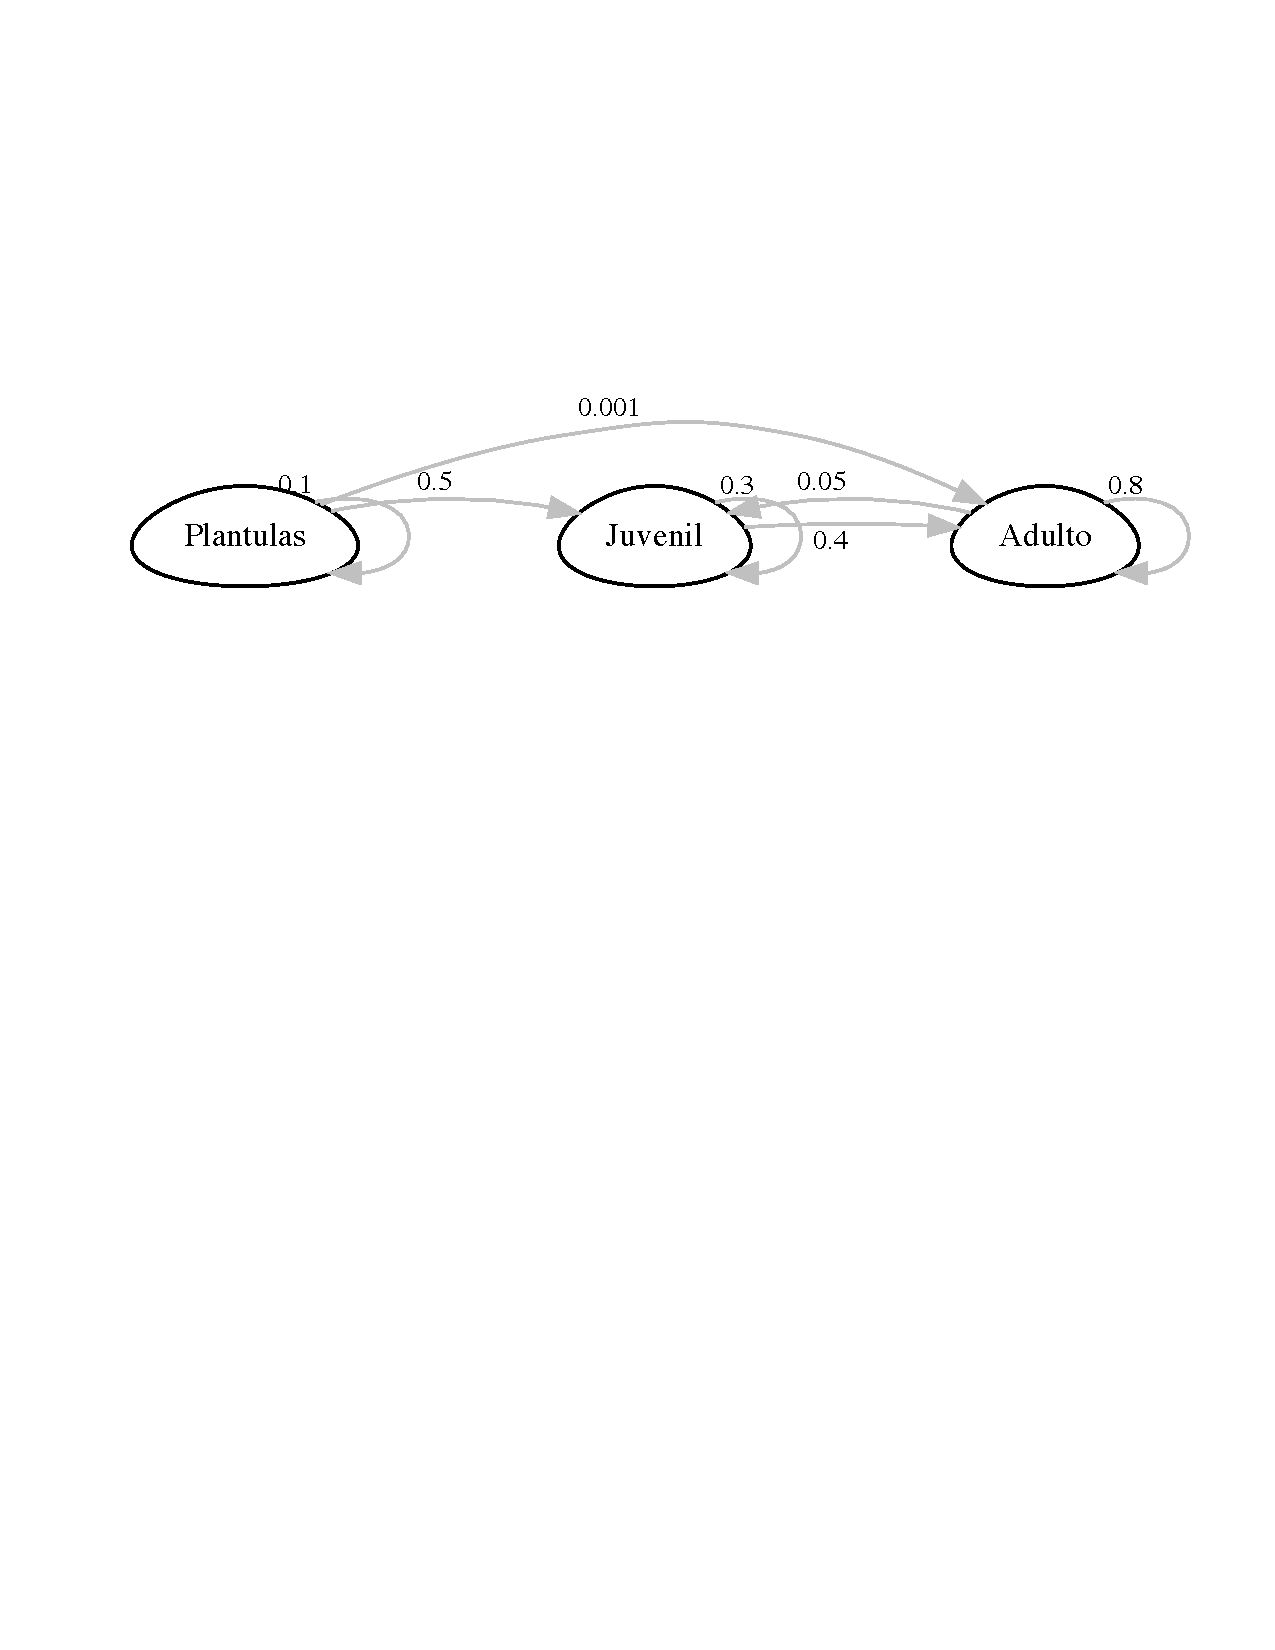
\includegraphics{Diagnostico_Poblacional_files/figure-latex/chap6_1-1.pdf}

\section{MatF: Matriz de fecundidad}\label{matf-matriz-de-fecundidad}

Si uno sigue la figura anterior vemos que los individuos en la segunda etapa se reproducen sexualmente (producen plantulas). Por consequencia seria probablemente más adecuado cambiar de nombre para la segunda etapa de ``juvenil'' a ``individuos pequeños''. Lo que se observa es el ciclo de vida de la oportaciones de plantulas es que los Individuos pequeños y Grande producen plantulas.

\begin{Shaded}
\begin{Highlighting}[]
\FunctionTok{library}\NormalTok{(DiagrammeR)}
\FunctionTok{library}\NormalTok{(Rage)}
\NormalTok{matF }\OtherTok{\textless{}{-}} \FunctionTok{rbind}\NormalTok{(}
  \FunctionTok{c}\NormalTok{(}\FloatTok{0.0}\NormalTok{, }\FloatTok{0.4}\NormalTok{, }\FloatTok{1.8}\NormalTok{),}
  \FunctionTok{c}\NormalTok{(}\FloatTok{0.0}\NormalTok{, }\FloatTok{0.0}\NormalTok{, }\FloatTok{0.0}\NormalTok{),}
  \FunctionTok{c}\NormalTok{(}\FloatTok{0.0}\NormalTok{, }\FloatTok{0.0}\NormalTok{, }\FloatTok{0.0}\NormalTok{)}
\NormalTok{)}
\NormalTok{stages }\OtherTok{\textless{}{-}} \FunctionTok{c}\NormalTok{(}\StringTok{"Plantulas"}\NormalTok{, }\StringTok{"Ind Pequeños"}\NormalTok{, }\StringTok{"Ind Grande"}\NormalTok{)}
\FunctionTok{plot\_life\_cycle}\NormalTok{(matF, }\AttributeTok{stages=}\NormalTok{stages)}
\end{Highlighting}
\end{Shaded}

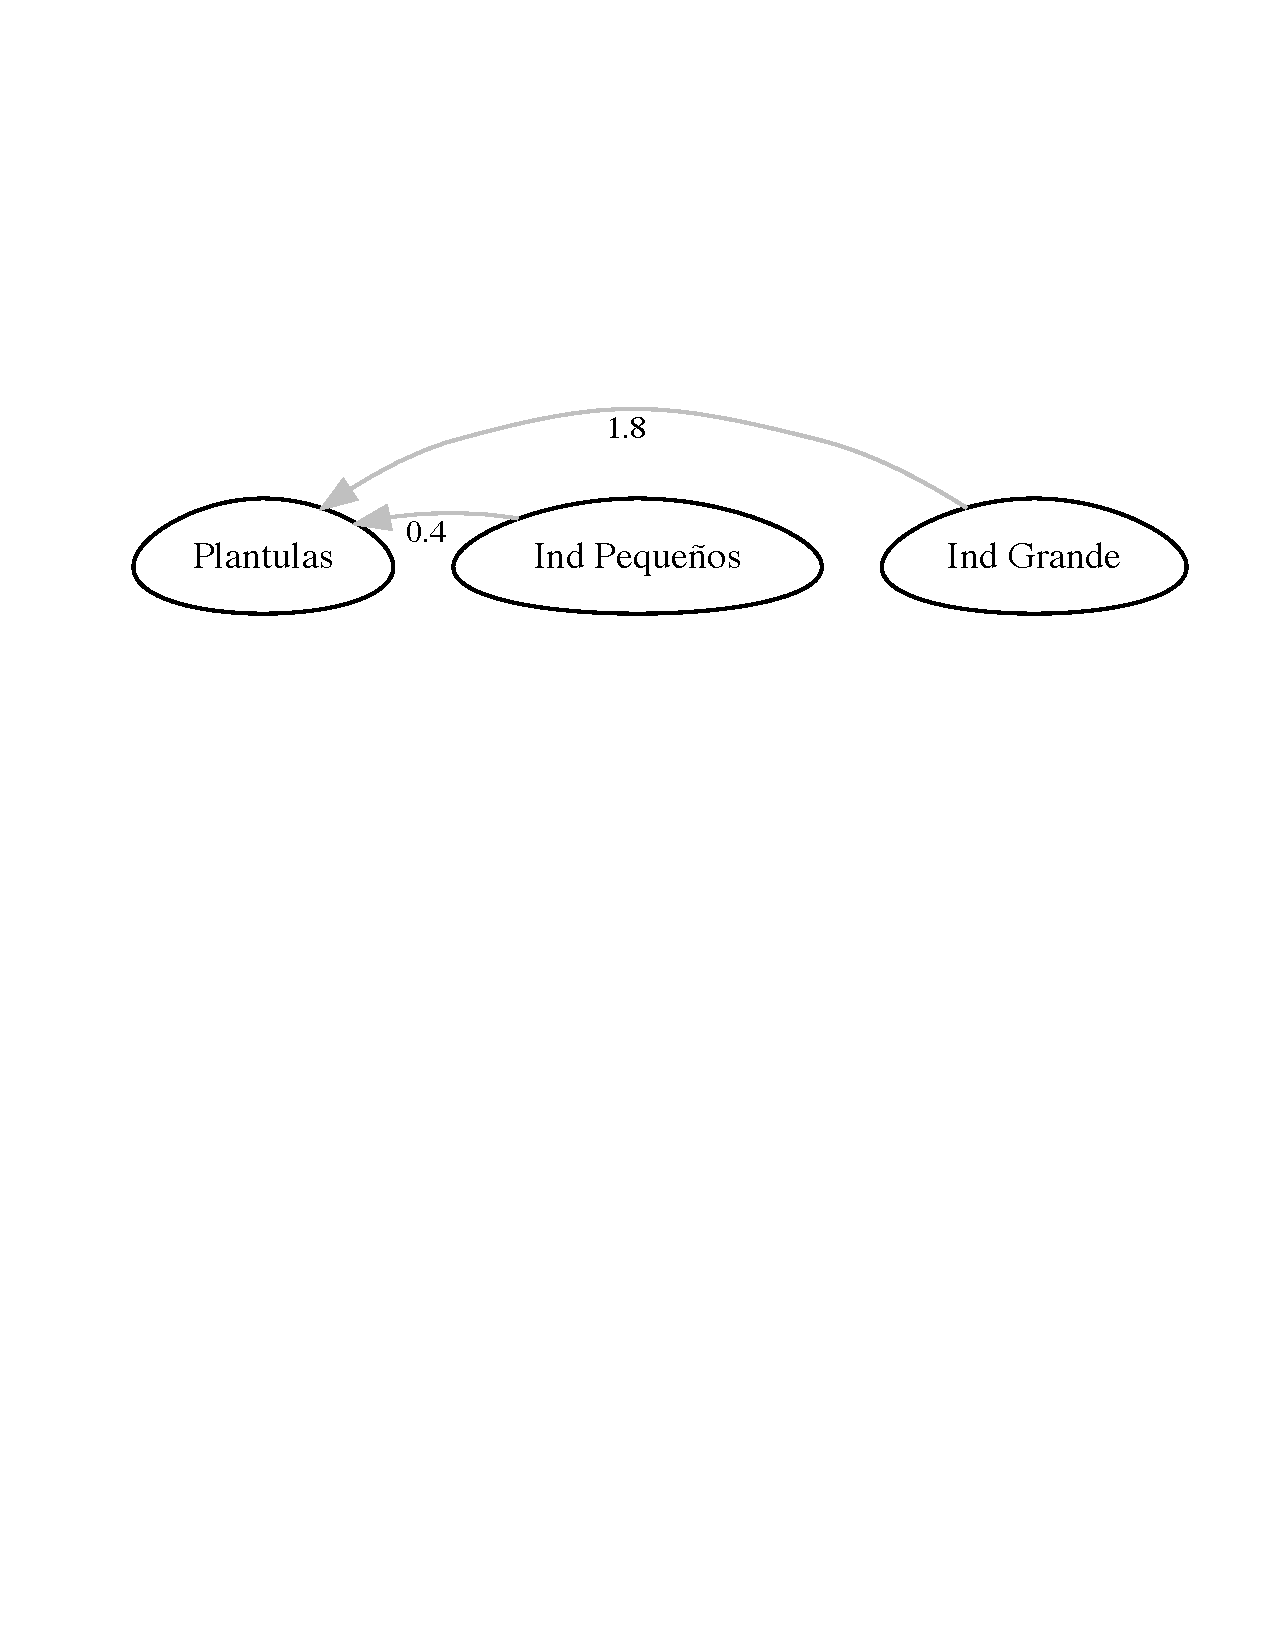
\includegraphics{Diagnostico_Poblacional_files/figure-latex/chap6_2-1.pdf}

\section{MatC = Matriz de clonación}\label{matc-matriz-de-clonaciuxf3n}

Esa matriz representa la información para especies que se reproducen por clonaje. Nota que hay necesitar de definir lo que es crecimiento por clonaje. Por ejemplo un individuo de \emph{Epidendrum} que crece y que tenga más tallos, no debería ser considerado clonaje, pero crecimiento del individuo. Al contrario un individuo que crece de forma que la planta madre se separa en dos o más partes donde no comparten conexión pudiese ser considerado clonaje. Otra alternativa es que hay muchas especies de orquídeas que producen \emph{keiki}, el momento que estos se separan de la madre se pueden considerar como el mismo individuo (geneticamente igual) a parte (ecologicamente distincto).

Necesitamos fotos de orquídeas con clonaje y keiki (quien puede ayudar)

Se debería enfatizar que añadir el concepto de clonaje dentro de la matriz de transiones resulta en estimados de parámetros diferentes, tal como el tamaño efectivo de población, Ne, en adición de evaluar otros conceptos evolutivos. En estudios evolutivos no es el individuo como tal que es la unidad de interés pero el individuo como fuente de diversidad genética, por consecuencia individuos (clones) que son genéticamente igual son evolutivamente el mismo individuos aunque estén separado físicamente. Las poblaciones organizados en clones afecta la interpretación de datos tanto en los estudios ecológico y evolutivos \citet{cook1983clonal}. Cuando se estudia especies con clonación hay que diferenciar entre los que es el ``ramet'' y un ``genet''. Los ``genets'' son la suma de todas las partes ``los ramets'' que tiene la misma genética. Los ``ramet'', son las partes individuales del individuo. En orquídea se podría considerar cada seudobulbo como un ramet y la suma de todos los seudobulbo como el ``genet''. Hay acercamiento para tomar en cuenta la adecuación de los ``individuos'' en la matriz y por consecuencia intergrar el concepto de clonación en los estimados. vea: \citet{mcgraw1996estimation}.

\chapter{Método bayesiano de calcular las transciones y fecundidades}\label{muxe9todo-bayesiano-de-calcular-las-transciones-y-fecundidades}

Por: Raymond L. Tremblay

El objetivo de este capítulo es demostrar algunos de los retos cuando uno trabaja con especies raras o con especies que tiene tamaño de muestra limitada. El onjetivo de este capitulo es demostrar como tomar encuenta los analisis cuando hay poca información para estimar los parametros de la matrices y como se puede resolver y estimar parametros más realista.

Considera este primer ejemplo donde se estima que la especie de interes tenga tres etapas en su ciclo de vida (semillas, plantulas y adultos) y que solamente la etapa más grande (de adultez) puede producir semillas.

Cuando se comienza un analisis de dinamica poblacional el primer paso es evaluar y tratar de ver cual son las etapas del ciclo de vida que pudiesen ser representativo de la dinámica principal de la especie y que sea realista cuando se considera el ciclo de vida de la especies y práctico en la recolección de datos.

En esta primera figura vemos lo que se considerá que ocurre en esa especie hipotetica.

Ahora ud recoge los datos del campo y evalua las transiciones y fecundidad y tiene información siguiente.

\begin{enumerate}
\def\labelenumi{\arabic{enumi}.}
\tightlist
\item
  Todas las semilla germinan y crece a la etapa de plantula.\\
\end{enumerate}

\begin{itemize}
\tightlist
\item
  Es realista que todas las semillas germinan?
\item
  Por que no se encontró semillas que NO germinan?
\end{itemize}

\begin{enumerate}
\def\labelenumi{\arabic{enumi}.}
\setcounter{enumi}{1}
\tightlist
\item
  Todos las plantulas mueren

  \begin{itemize}
  \tightlist
  \item
    Es realista que todas las plantulas se muere dentro del ciclo de vida de una especies?
  \end{itemize}
\end{enumerate}

Aqui se ve dos de los problemas que resulta en MPM que no son realista, uno que no hay ninguna mortantad o que todo se muere. El otro componente es el efecto del tamaño de muestra, considerá que su especie de interes usted tuvo acceso solamente a 4 plantas adultas (un especies rara), y 4 de los 4 sobrevieron, por consecuencia 100\% de supervivencia. Si los individuos llegan a esta etapa son inmortales!!!? Claramente es un resultado del tamaño de muestra y no del ciclo de vida de la especie.

Es importante reconocer la diferencia entre los valores recolectado y la historia de vida típica de una especies. Uno podría usar los datos que 100\% de los individuos sobreviven pero eso es realista a largo plazo?

El paquete raretrans ayuda en resolver estos asuntos illogicos y crear matrices que son más realistas al considerar el ciclo de vida típica de la especie estudiada.

Aqui un ciclo de vida que no es biologicamente realista

\begin{itemize}
\tightlist
\item
  todas las semilla sobreviven y pasan a plantulas
\item
  ninguna plantula sobrevive y/o pasa a ser adultos
\item
  los adultos 90\% se quedan como adulto pero ninguno produce semillas
\end{itemize}

NOTA que es posible que los datos que recolectan del campo sean estos, pero muchas veces esas observaciones son un resultado de la falta de tamaño de muestra.

\begin{Shaded}
\begin{Highlighting}[]
\CommentTok{\# hidden code to produce figures}
\FunctionTok{library}\NormalTok{(DiagrammeR)}
\FunctionTok{library}\NormalTok{(Rage)}


\NormalTok{matA }\OtherTok{\textless{}{-}} \FunctionTok{rbind}\NormalTok{(}
  \FunctionTok{c}\NormalTok{(}\FloatTok{0.0}\NormalTok{, }\FloatTok{0.0}\NormalTok{, }\FloatTok{0.0}\NormalTok{),}
  \FunctionTok{c}\NormalTok{(}\FloatTok{1.0}\NormalTok{, }\FloatTok{0.0}\NormalTok{, }\FloatTok{0.0}\NormalTok{),}
  \FunctionTok{c}\NormalTok{(}\FloatTok{0.0}\NormalTok{, }\FloatTok{0.0}\NormalTok{, }\FloatTok{0.9}\NormalTok{)}
\NormalTok{)}
\NormalTok{stages }\OtherTok{\textless{}{-}} \FunctionTok{c}\NormalTok{(}\StringTok{"semillas"}\NormalTok{, }\StringTok{"plantulas"}\NormalTok{, }\StringTok{"adultos"}\NormalTok{)}
\NormalTok{title }\OtherTok{\textless{}{-}} \ConstantTok{NULL}
\end{Highlighting}
\end{Shaded}

\begin{Shaded}
\begin{Highlighting}[]
\FunctionTok{plot\_life\_cycle}\NormalTok{(matA, }\AttributeTok{stages=}\NormalTok{stages)}
\end{Highlighting}
\end{Shaded}

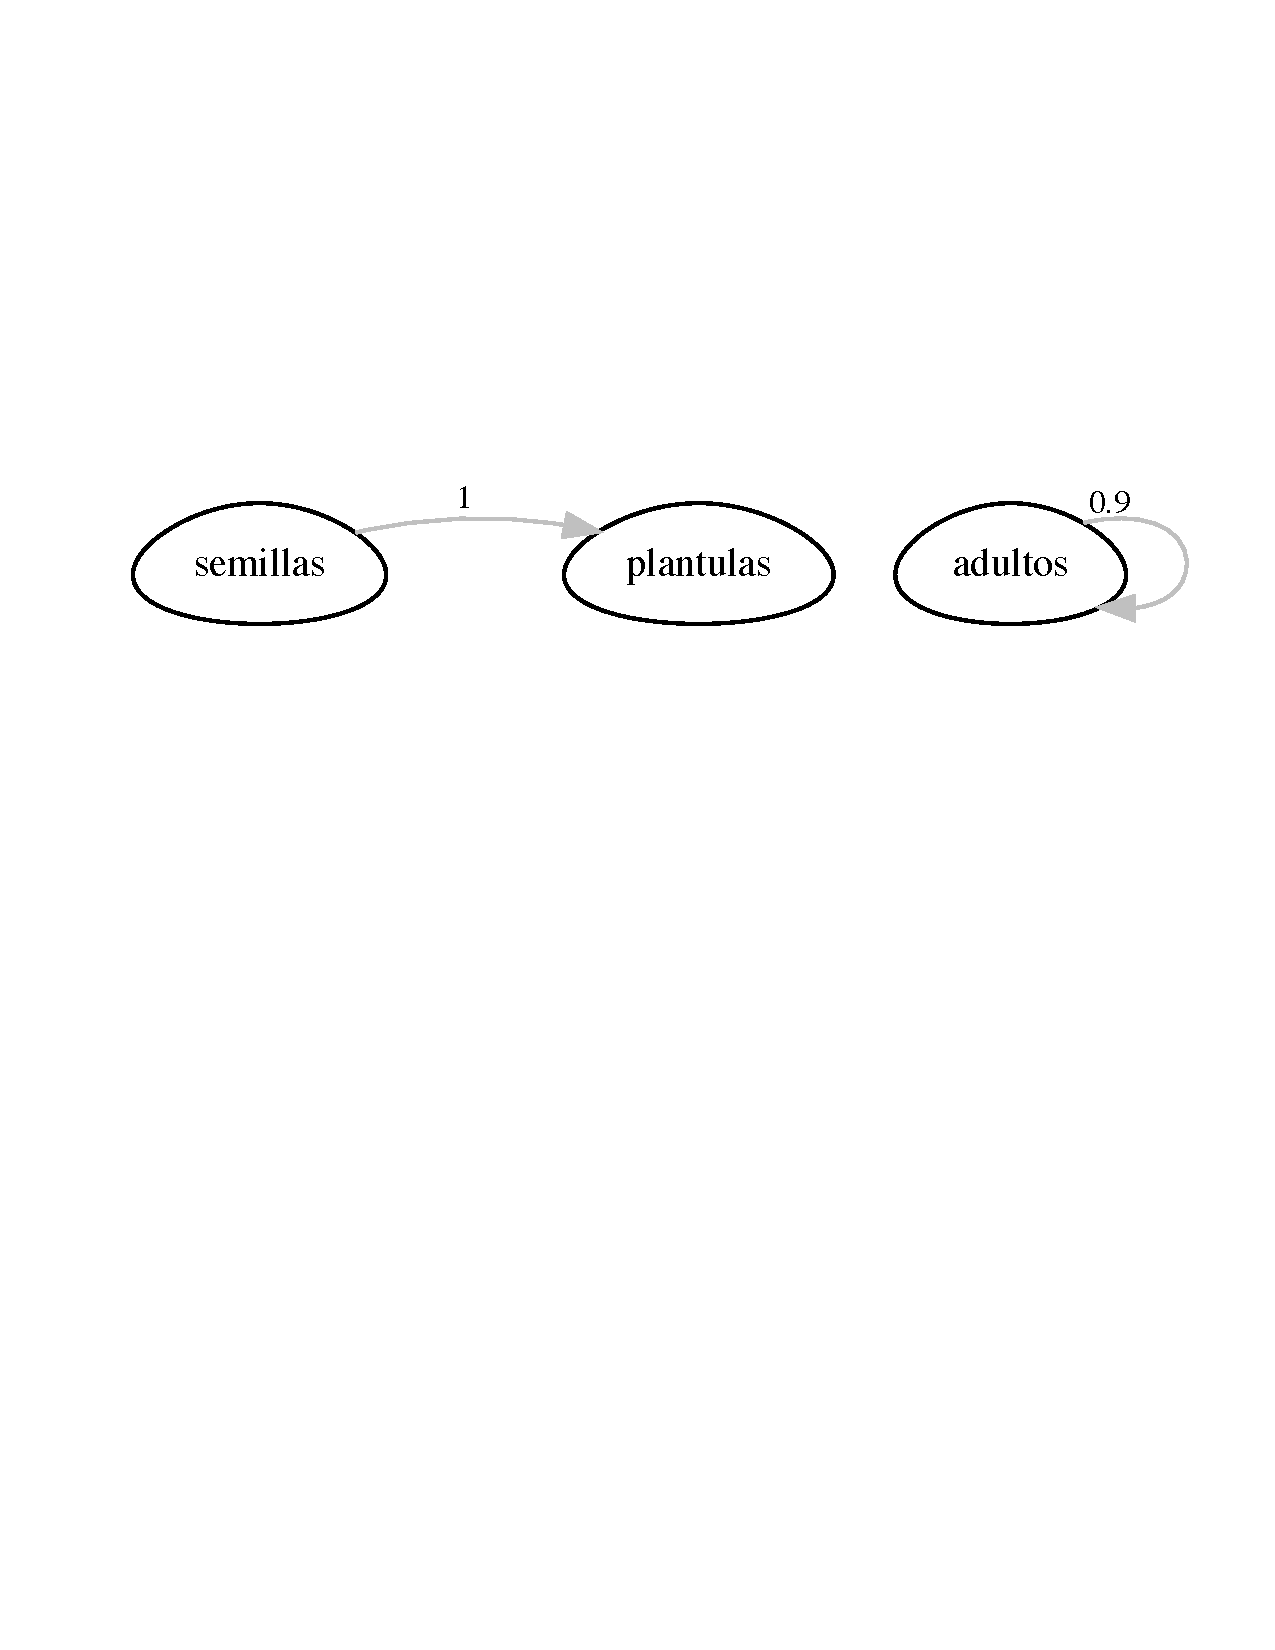
\includegraphics{Diagnostico_Poblacional_files/figure-latex/chap7_2-1.pdf}

Considera este ejemplo:

\begin{itemize}
\tightlist
\item
  Si Ud estudia los arboles Sequioa y muestra los arboles grandes (con un dbh de \textgreater{} xxx), aunque muestra 1000+ individuos de esa etapa/tamaño es posible que no encontrará ninguno que muere. Por consecuencia el estimado de supervivencia de esos arboles es 100\%. Aunque uno sabe que si hubiese muestrado 10,000 o 100,000 arboles se podria haber detectado uno más que fallece.
\end{itemize}

\section{El paquete ``raretrans''}\label{el-paquete-raretrans}

La información original del uso del paquete se encuentra aqui \url{https://doi.org/10.1016/j.ecolmodel.2021.109526}.

\textbf{Population projections from holey matrices: Using prior information to estimate rare transition events}

Abstracto

Las matrices de proyección de población son un medio común para predecir la persistencia de la población a corto y largo plazo para especies raras, amenazadas y en peligro de extinción. Los datos de tales especies pueden sufrir de tamaños de muestra pequeños y, en consecuencia, perder eventos demográficos raros que dan como resultado trayectorias de ciclo de vida incompletas o biológicamente poco realistas. Las matrices con valores faltantes (ceros; p.~ej., sin observación de semillas que se transforman en plántulas) a menudo se subsituyen utilizando información previa de la literatura, otras poblaciones, períodos de tiempo, otras especies, estimaciones de las mejores conjeturas o, a veces, incluso se ignoran. Para paliar este problema, proponemos usar un modelo multinomial de Dirichlet para parametrizar transiciones y un Gamma para los estimados de reproducción para substituir los valores faltantes en estas matrices perforadas. Esto integra formalmente la información previa dentro de un marco bayesiano e incluye explícitamente el peso de la información previa en las distribuciones posteriores. Mostramos utilizando dos conjuntos de datos reales que el peso asignado a la información anterior influye principalmente en la dispersión de los posteriores, la inclusión de anteriores da como resultado matrices irreducibles y ergódicas, y se pueden hacer inferencias biológicamente más realistas sobre las probabilidades de transición. Debido a que las previas se establecen explícitamente, los resultados son reproducibles y se pueden volver a evaluar si hay previas alternas disponibles en el futuro.

\section{Instalación de los paquetes \#1}\label{instalaciuxf3n-de-los-paquetes-1}

\begin{Shaded}
\begin{Highlighting}[]
\ControlFlowTok{if}\NormalTok{ (}\SpecialCharTok{!}\FunctionTok{require}\NormalTok{(}\StringTok{"pacman"}\NormalTok{)) }\FunctionTok{install.packages}\NormalTok{(}\StringTok{"pacman"}\NormalTok{)}
\end{Highlighting}
\end{Shaded}

\begin{verbatim}
## Loading required package: pacman
\end{verbatim}

\begin{Shaded}
\begin{Highlighting}[]
\NormalTok{pacman}\SpecialCharTok{::}\FunctionTok{p\_load}\NormalTok{(janitor, tidyverse, devtools)}

\FunctionTok{library}\NormalTok{(tidyverse)}
\FunctionTok{library}\NormalTok{(janitor)}
\end{Highlighting}
\end{Shaded}

\section{Instalación de raretrans \#2}\label{instalaciuxf3n-de-raretrans-2}

Para instalar \textbf{raretrans} remover el \textbf{\#} antes de correr el script para tener aceco a los codigos de \textbf{raretrans}.

\begin{Shaded}
\begin{Highlighting}[]
\CommentTok{\#library(devtools)}

\NormalTok{devtools}\SpecialCharTok{::}\FunctionTok{install\_github}\NormalTok{(}\StringTok{"atyre2/raretrans"}\NormalTok{, }\AttributeTok{build =} \ConstantTok{TRUE}\NormalTok{, }\AttributeTok{build\_opts =} \FunctionTok{c}\NormalTok{(}\StringTok{"{-}{-}no{-}resave{-}data"}\NormalTok{, }\StringTok{"{-}{-}no{-}manual"}\NormalTok{))}
\end{Highlighting}
\end{Shaded}

\begin{verbatim}
## Skipping install of 'raretrans' from a github remote, the SHA1 (3cbc441c) has not changed since last install.
##   Use `force = TRUE` to force installation
\end{verbatim}

\begin{Shaded}
\begin{Highlighting}[]
\FunctionTok{library}\NormalTok{(raretrans)}
\end{Highlighting}
\end{Shaded}

Vea el siguiente website para más información en ingles, la información que sigue es una traducción y ampliación de la información en el siuiente enlace.

\url{https://atyre2.github.io/raretrans/articles/onepopperiod.html}

\begin{Shaded}
\begin{Highlighting}[]
\FunctionTok{library}\NormalTok{(tidyverse)}
\FunctionTok{library}\NormalTok{(ggplot2)}
\FunctionTok{library}\NormalTok{(popbio) }\CommentTok{\# para la función projection.matrix()}
\FunctionTok{library}\NormalTok{(raretrans)}
\CommentTok{\# Mi tema de ggplot2 personal}
\NormalTok{rlt\_theme }\OtherTok{\textless{}{-}} \FunctionTok{theme}\NormalTok{(}\AttributeTok{axis.title.y =} \FunctionTok{element\_text}\NormalTok{(}\AttributeTok{colour=}\StringTok{"grey20"}\NormalTok{,}\AttributeTok{size=}\DecValTok{15}\NormalTok{,}\AttributeTok{face=}\StringTok{"bold"}\NormalTok{),}
        \AttributeTok{axis.text.x =} \FunctionTok{element\_text}\NormalTok{(}\AttributeTok{colour=}\StringTok{"grey20"}\NormalTok{,}\AttributeTok{size=}\DecValTok{15}\NormalTok{, }\AttributeTok{face=}\StringTok{"bold"}\NormalTok{),}
        \AttributeTok{axis.text.y =} \FunctionTok{element\_text}\NormalTok{(}\AttributeTok{colour=}\StringTok{"grey20"}\NormalTok{,}\AttributeTok{size=}\DecValTok{15}\NormalTok{,}\AttributeTok{face=}\StringTok{"bold"}\NormalTok{),  }
        \AttributeTok{axis.title.x =} \FunctionTok{element\_text}\NormalTok{(}\AttributeTok{colour=}\StringTok{"grey20"}\NormalTok{,}\AttributeTok{size=}\DecValTok{15}\NormalTok{,}\AttributeTok{face=}\StringTok{"bold"}\NormalTok{))}
\end{Highlighting}
\end{Shaded}

El objetivo de esta viñeta es demostrar el uso del paquete \texttt{raretrans}
para los calculos de los parametros en una población y periodo de
transición.

\section{Parte I: Obtención de la matriz de proyección}\label{parte-i-obtenciuxf3n-de-la-matriz-de-proyecciuxf3n}

\texttt{raretrans} asume que la matriz de proyección es una lista de dos
matrices, una matriz de transición y una matriz de fertilidad. Este es
el formato de salida de \texttt{popbio::projection.matrix}. Si tenemos
transiciones individuales en un marco de datos

Podemos utilizar \texttt{popbio::projection.matrix} para obtener los datos
necesarios. Hacemos una demostración con los datos de transición y
fertilidad de la orquídea epifita \emph{Lepanthes elto} \textbf{POPNUM 250} en el
\textbf{periodo 5}. \emph{Lepanthes eltoroensis} es endemica de Puerto Rico, epifita y limitada a una pequeña región de la isla.

\section{\texorpdfstring{Paso 1: Cargar y fusionar los datos de población única para \emph{L. elto}}{Paso 1: Cargar y fusionar los datos de población única para L. elto}}\label{paso-1-cargar-y-fusionar-los-datos-de-poblaciuxf3n-uxfanica-para-l.-elto}

\begin{Shaded}
\begin{Highlighting}[]
\FunctionTok{data}\NormalTok{(}\StringTok{"L\_elto"}\NormalTok{) }\CommentTok{\# carga el conjunto de datos \textasciigrave{}L\_elto\textasciigrave{} en la memoria de la computadora (los datos están incluido en el paquete \textasciigrave{}raretrans\textasciigrave{})}
\FunctionTok{head}\NormalTok{(L\_elto) }
\end{Highlighting}
\end{Shaded}

\begin{verbatim}
## # A tibble: 6 x 13
##   POPNUM  year seedlings adults fertility IND_NUM stage next_stage first_year
##    <dbl> <dbl>     <dbl>  <dbl>     <dbl>   <dbl> <chr> <chr>           <dbl>
## 1    209     1         1      6         0      67 j     j                   1
## 2    209     1         1      6         0      68 a     a                   1
## 3    209     1         1      6         0      69 a     a                   1
## 4    209     1         1      6         0      70 a     a                   1
## 5    209     1         1      6         0      71 j     a                   1
## 6    209     1         1      6         0      72 a     a                   1
## # i 4 more variables: last_year <dbl>, recruited <lgl>, died <dbl>,
## #   lifespan <int>
\end{verbatim}

\section{Organización de los datos en el ``data.frame''}\label{organizaciuxf3n-de-los-datos-en-el-data.frame}

\begin{itemize}
\tightlist
\item
  el primer paso es seleccionar los datos de una población y un periodo de tiempo.
\item
  el segundo paso es hacer un cambio en la terminología para el estado más pequeño de ``plantula'' a ``seedling''\ldots{} Ese cambio es para que la información presentada aqui sea la misma que en el documento en ingles.
\end{itemize}

Cada fila de este data.frame de datos tiene columnas para la fase actual (stage, periodo \textbf{t}), la fase siguiente (next\_stage, periodo \textbf{t+1}) y la fertilidad por individuo.
Tenga en cuenta que ``p'' significa ``plantula'' en español. El primer conjunto de líneas de abajo cambia el nombre de la etapa del ciclo vital de ``p'' a ``s'' después de seleccionar la población y el periodo de tiempo.

\begin{Shaded}
\begin{Highlighting}[]
\NormalTok{onepop }\OtherTok{\textless{}{-}}\NormalTok{ L\_elto }\SpecialCharTok{\%\textgreater{}\%}   
\CommentTok{\# Filtrar la población \# 250, el periodo (año=year) 5}
  \FunctionTok{filter}\NormalTok{(POPNUM }\SpecialCharTok{==} \DecValTok{250}\NormalTok{, year }\SpecialCharTok{==} \DecValTok{5}\NormalTok{) }\SpecialCharTok{\%\textgreater{}\%} 
  \CommentTok{\# redefine "p" por plantula a "s" para seedling}
  \FunctionTok{mutate}\NormalTok{(}\AttributeTok{stage =} \FunctionTok{case\_when}\NormalTok{(stage }\SpecialCharTok{==} \StringTok{"p"} \SpecialCharTok{\textasciitilde{}} \StringTok{"s"}\NormalTok{,}
                           \ConstantTok{TRUE} \SpecialCharTok{\textasciitilde{}}\NormalTok{ stage),}
         \AttributeTok{next\_stage =} \FunctionTok{case\_when}\NormalTok{(next\_stage }\SpecialCharTok{==} \StringTok{"p"}\SpecialCharTok{\textasciitilde{}} \StringTok{"s"}\NormalTok{,}
                                \ConstantTok{TRUE} \SpecialCharTok{\textasciitilde{}}\NormalTok{ next\_stage))}
\CommentTok{\# popbio::projection.matrix no funciona con tibbles, por consecuencia se convierte en data.frame}

\FunctionTok{head}\NormalTok{(onepop) }\CommentTok{\# AHora tenemos solamente datos de la población \#250 del periodo 5}
\end{Highlighting}
\end{Shaded}

\begin{verbatim}
## # A tibble: 6 x 13
##   POPNUM  year seedlings adults fertility IND_NUM stage next_stage first_year
##    <dbl> <dbl>     <dbl>  <dbl>     <dbl>   <dbl> <chr> <chr>           <dbl>
## 1    250     5         8     34     0         167 j     a                   1
## 2    250     5         8     34     0         168 j     a                   1
## 3    250     5         8     34     0         169 j     a                   1
## 4    250     5         8     34     0.118     170 a     a                   1
## 5    250     5         8     34     0         172 j     j                   1
## 6    250     5         8     34     0         173 j     a                   1
## # i 4 more variables: last_year <dbl>, recruited <lgl>, died <dbl>,
## #   lifespan <int>
\end{verbatim}

\begin{Shaded}
\begin{Highlighting}[]
\CommentTok{\# Crear TF = TRUE, añadir para formatear corectamente.}
\NormalTok{TF }\OtherTok{\textless{}{-}}\NormalTok{ popbio}\SpecialCharTok{::}\FunctionTok{projection.matrix}\NormalTok{(}\FunctionTok{as.data.frame}\NormalTok{(onepop), }
                        \AttributeTok{stage =}\NormalTok{ stage, }\AttributeTok{fate =}\NormalTok{ next\_stage, }
                        \AttributeTok{fertility=}\StringTok{"fertility"}\NormalTok{, }\AttributeTok{sort=}\FunctionTok{c}\NormalTok{(}\StringTok{"s"}\NormalTok{,}\StringTok{"j"}\NormalTok{,}\StringTok{"a"}\NormalTok{), }\AttributeTok{TF =} \ConstantTok{TRUE}\NormalTok{)}
\NormalTok{TF }\CommentTok{\# Este es la estructura de etapas de vida para esa población.  Nota que tenemos dos matrices, una de transiciones **T** y otra de fertilidad **F**. }
\end{Highlighting}
\end{Shaded}

\begin{verbatim}
## $T
##    
##              s          j          a
##   s 0.09090909 0.00000000 0.00000000
##   j 0.63636364 0.57446809 0.00000000
##   a 0.00000000 0.29787234 0.85294118
## 
## $F
##    
##             s         j         a
##   s 0.0000000 0.0000000 0.1176471
##   j 0.0000000 0.0000000 0.0000000
##   a 0.0000000 0.0000000 0.0000000
\end{verbatim}

\section{Nota:}\label{nota}

Nuestros estadios se codifican ahora como \textbf{s} (plántula), \textbf{j} (juvenil) y \textbf{a} (adulto), y ahora tenemos dos matrices: \textbf{T} (transición de estadios) y \textbf{F} (fecundidad). La tasa de crecimiento asintótico de la población observada es \(\lambda =\) 0.93. Las transiciones raras que faltan en nuestra primera matriz de transición, \texttt{TF\$T}, son la transición de plántula (\emph{s}) a adulto (\emph{a}) y la transición de \emph{j} a
\emph{s}. Pero sabemos que ocurren.

\section{Paso 2: Obtener el número inicial de individuos por etapa}\label{paso-2-obtener-el-nuxfamero-inicial-de-individuos-por-etapa}

Dado que nuestras recuentos (número de individuos, \emph{N}) y el tamaño de \emph{muestreo equivalente} a priori se expresa como múltiplo del número de individuos observados, necesitamos obtener el número de individuos en cada etapa (\(N\)) en el primer periodo de tiempo.

Utilizamos la función \texttt{raretrans::get\_state\_vector()} para obtener el recuento inicial de individuos, \emph{N}.

\begin{Shaded}
\begin{Highlighting}[]
\NormalTok{N }\OtherTok{\textless{}{-}} \FunctionTok{get\_state\_vector}\NormalTok{(onepop, }\AttributeTok{stage =}\NormalTok{ stage, }\AttributeTok{sort=}\FunctionTok{c}\NormalTok{(}\StringTok{"s"}\NormalTok{,}\StringTok{"j"}\NormalTok{,}\StringTok{"a"}\NormalTok{)) }
\NormalTok{N }\CommentTok{\# Un vector \# de individuos iniciales para cada etapa, nota que la cantidad por etapa, "stage", son los individuos en el primer muestreo}
\end{Highlighting}
\end{Shaded}

\begin{verbatim}
## [1] 11 47 34
\end{verbatim}

La lista de matrices y el vector de cuento de individuales no tienen por qué proceder de un data.frame como hemos hecho aquí. Mientras tengan el formato esperado, pueden crearse a mano. Usamos la población 231 en el periodo 2 como ejemplo, dividiendo la matriz en submatrices de transición \textbf{T} y fecundidad \textbf{F}. Abajo, \emph{m} significa ``muerte'', es decir, plantas que están muertas.

\begin{Shaded}
\begin{Highlighting}[]
\NormalTok{TF2}
\end{Highlighting}
\end{Shaded}

\begin{verbatim}
## $Tmat
##     stage
## fate         p         j         a
##    p 0.5000000 0.0000000 0.0000000
##    j 0.0000000 0.8333333 0.0000000
##    a 0.0000000 0.0625000 0.8750000
## 
## $Fmat
##      [,1] [,2]  [,3]
## [1,]    0    0 0.125
## [2,]    0    0 0.000
## [3,]    0    0 0.000
\end{verbatim}

\begin{Shaded}
\begin{Highlighting}[]
\NormalTok{N2}
\end{Highlighting}
\end{Shaded}

\begin{verbatim}
##  p  j  a 
##  2  6 16
\end{verbatim}

¿Como se ve el ciclo de vida de esa población en ese periodo?

\begin{Shaded}
\begin{Highlighting}[]
\NormalTok{stages2 }\OtherTok{\textless{}{-}} \FunctionTok{c}\NormalTok{(}\StringTok{"plantulas"}\NormalTok{, }\StringTok{"juveniles"}\NormalTok{, }\StringTok{"adultos"}\NormalTok{)}
\NormalTok{title }\OtherTok{\textless{}{-}} \ConstantTok{NULL}
\FunctionTok{plot\_life\_cycle}\NormalTok{(Tmat, }\AttributeTok{stages=}\NormalTok{stages2)}
\end{Highlighting}
\end{Shaded}

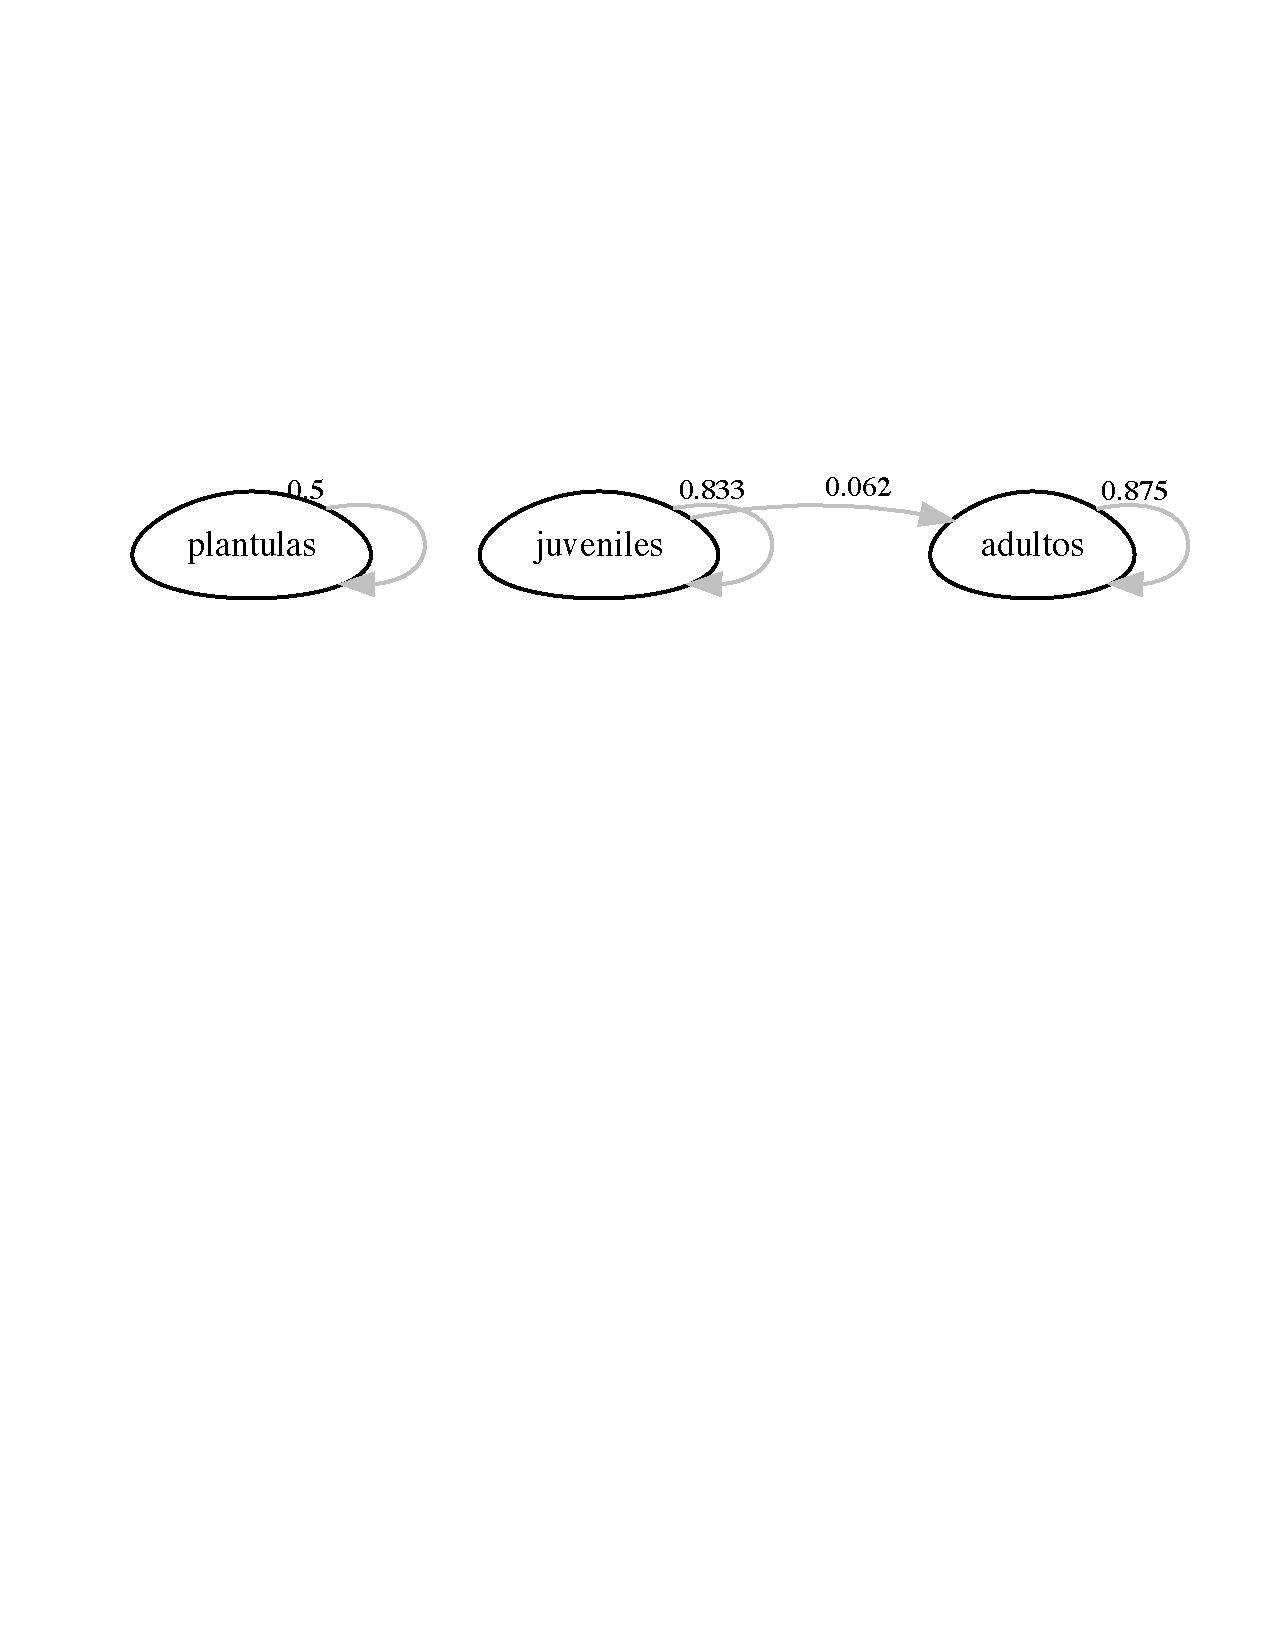
\includegraphics{Diagnostico_Poblacional_files/figure-latex/chap7_11-1.pdf}

En esta matriz falta la transición de plántula a juvenil, y ninguno de los 6 juveniles murió, lo que lleva a una sobreestimación de la supervivencia. La tasa de crecimiento asintótico de la población observada es \(\lambda =\) 0.88. La matriz no es ergódica (no se puede llegar a cualquier otro estado desde uno o más estados), y reducible, lo que significa que una o más columnas y filas se pueden descartar y tienen las mismas propiedades eigen.

\section{Parte 2: Uso de priors para incorporar transiciones raras}\label{parte-2-uso-de-priors-para-incorporar-transiciones-raras}

\subsection{Use priors no informativos}\label{use-priors-no-informativos}

\begin{itemize}
\tightlist
\item
  Ese paso es solamente para entender porque no se calcula y porque no
  se usa \emph{prior} uniforme.
\end{itemize}

Tremblay (\citet{tremblay2021population}) muestran que los valores de \emph{prior}
de una dirichlet funciona para las columnas de la matriz de transición
(\textbf{T}) y que valores \emph{prior} gamma funciona para las columnas de la
matriz de transición (\textbf{F}).

\subsection{Matriz de transición}\label{matriz-de-transiciuxf3n}

Por lo tanto, vamos a añadir un dirichlet uniforme con prior con un peso
= \(1\) a la matriz de transición, \(T\). Aquí, tenemos 4 destinos (3 +
muerte), por lo que cada destino 0,25 a la matriz de destinos
\emph{observados} (¡no a la matriz de transiciones!). de transición). Cuando
especificamos una matriz con un prior para las transiciones, hay una
fila más que columnas. Esta fila extra representa la muerte.

\begin{Shaded}
\begin{Highlighting}[]
\NormalTok{Tprior }\OtherTok{\textless{}{-}} \FunctionTok{matrix}\NormalTok{(}\FloatTok{0.25}\NormalTok{, }\AttributeTok{byrow =} \ConstantTok{TRUE}\NormalTok{, }\AttributeTok{ncol =} \DecValTok{3}\NormalTok{, }\AttributeTok{nrow=}\DecValTok{4}\NormalTok{)}
\FunctionTok{fill\_transitions}\NormalTok{(TF, N, }\AttributeTok{P =}\NormalTok{ Tprior) }\CommentTok{\# resultado de la matriz de transición básica}
\end{Highlighting}
\end{Shaded}

\begin{verbatim}
##            [,1]        [,2]        [,3]
## [1,] 0.10416667 0.005208333 0.007142857
## [2,] 0.60416667 0.567708333 0.007142857
## [3,] 0.02083333 0.296875000 0.835714286
\end{verbatim}

\begin{Shaded}
\begin{Highlighting}[]
\CommentTok{\# Para entender las diferencias compara los resultados con *$T* del objeto *TF*}
\NormalTok{TF}
\end{Highlighting}
\end{Shaded}

\begin{verbatim}
## $T
##    
##              s          j          a
##   s 0.09090909 0.00000000 0.00000000
##   j 0.63636364 0.57446809 0.00000000
##   a 0.00000000 0.29787234 0.85294118
## 
## $F
##    
##             s         j         a
##   s 0.0000000 0.0000000 0.1176471
##   j 0.0000000 0.0000000 0.0000000
##   a 0.0000000 0.0000000 0.0000000
\end{verbatim}

\subsection{Como calcular a mano!}\label{como-calcular-a-mano}

Podemos obtener el mismo resultado `a mano' - necesitamos el vector de
observaciones porque la posterior se calcula a partir de las
observaciones de transiciones, no la matriz de transiciones.

\begin{Shaded}
\begin{Highlighting}[]
\NormalTok{Tobs }\OtherTok{\textless{}{-}} \FunctionTok{sweep}\NormalTok{(TF}\SpecialCharTok{$}\NormalTok{T, }\DecValTok{2}\NormalTok{, N, }\StringTok{"*"}\NormalTok{) }\CommentTok{\# obtener las observaciones de transiciones }
\NormalTok{Tobs }\OtherTok{\textless{}{-}} \FunctionTok{rbind}\NormalTok{(Tobs, N }\SpecialCharTok{{-}} \FunctionTok{colSums}\NormalTok{(Tobs)) }\CommentTok{\# añadir la fila de muerte }
\NormalTok{Tobs }\OtherTok{\textless{}{-}}\NormalTok{ Tobs }\SpecialCharTok{+} \FloatTok{0.25} \CommentTok{\# añadir los prior}
\FunctionTok{sweep}\NormalTok{(Tobs, }\DecValTok{2}\NormalTok{, }\FunctionTok{colSums}\NormalTok{(Tobs), }\StringTok{"/"}\NormalTok{)[}\SpecialCharTok{{-}}\DecValTok{4}\NormalTok{,] }\CommentTok{\# dividir por la suma de la column y descarta la fila de muerte }
\end{Highlighting}
\end{Shaded}

\begin{verbatim}
##            s           j           a
## s 0.10416667 0.005208333 0.007142857
## j 0.60416667 0.567708333 0.007142857
## a 0.02083333 0.296875000 0.835714286
\end{verbatim}

El \emph{prior uniforme} rellena las transiciones que faltan, pero también
crea problemas porque proporciona valores de transición que son
biológicamente imposibles. Por ejemplo, proporciona una transición para
adulto-\textgreater plántula, cuando esta transición sólo es posible en la matriz
de fecundidad \(F\). Por esta razón, no recomendamos el uso de priores
uniformes. En otra palabra usando un prior uniforme no toma en cuenta el
ciclo de vida de una especie.

\subsection{Matriz de fecundidad}\label{matriz-de-fecundidad}

Debemos especificar los parámetros para la fertilidad \emph{a priori} como
una matriz. Las etapas que no hay reproducción o sea que no se producen
por reproducción deben ser \texttt{NA}, usando \emph{NA\_real\_}. El concepto de
\emph{NA\_real\_} es que es un valor que no esta presente pero con puntos
decimales. Nota que el valor de \emph{prior} de la fertilidad es 0.0001.

\begin{Shaded}
\begin{Highlighting}[]
\NormalTok{alpha }\OtherTok{\textless{}{-}} \FunctionTok{matrix}\NormalTok{(}\FunctionTok{c}\NormalTok{(}\ConstantTok{NA\_real\_}\NormalTok{, }\ConstantTok{NA\_real\_}\NormalTok{, }\FloatTok{1e{-}5}\NormalTok{,}
                  \ConstantTok{NA\_real\_}\NormalTok{, }\ConstantTok{NA\_real\_}\NormalTok{, }\ConstantTok{NA\_real\_}\NormalTok{,}
                  \ConstantTok{NA\_real\_}\NormalTok{, }\ConstantTok{NA\_real\_}\NormalTok{, }\ConstantTok{NA\_real\_}\NormalTok{), }\AttributeTok{nrow=}\DecValTok{3}\NormalTok{, }\AttributeTok{ncol =} \DecValTok{3}\NormalTok{, }\AttributeTok{byrow =} \ConstantTok{TRUE}\NormalTok{)}
\NormalTok{beta }\OtherTok{\textless{}{-}} \FunctionTok{matrix}\NormalTok{(}\FunctionTok{c}\NormalTok{(}\ConstantTok{NA\_real\_}\NormalTok{, }\ConstantTok{NA\_real\_}\NormalTok{, }\FloatTok{1e{-}5}\NormalTok{,}
                  \ConstantTok{NA\_real\_}\NormalTok{, }\ConstantTok{NA\_real\_}\NormalTok{, }\ConstantTok{NA\_real\_}\NormalTok{,}
                  \ConstantTok{NA\_real\_}\NormalTok{, }\ConstantTok{NA\_real\_}\NormalTok{, }\ConstantTok{NA\_real\_}\NormalTok{), }\AttributeTok{nrow=}\DecValTok{3}\NormalTok{, }\AttributeTok{ncol =} \DecValTok{3}\NormalTok{, }\AttributeTok{byrow =} \ConstantTok{TRUE}\NormalTok{)}
\FunctionTok{fill\_fertility}\NormalTok{(TF, N, }\AttributeTok{alpha =}\NormalTok{ alpha, }\AttributeTok{beta =}\NormalTok{ beta)}
\end{Highlighting}
\end{Shaded}

\begin{verbatim}
##    
##             s         j         a
##   s 0.0000000 0.0000000 0.1176473
##   j 0.0000000 0.0000000 0.0000000
##   a 0.0000000 0.0000000 0.0000000
\end{verbatim}

El cambio en la fertilidad es \textless{} 0,0001 en comparación con el valor
observado.

\subsection{Calculando los Priors de fertilidad a mano}\label{calculando-los-priors-de-fertilidad-a-mano}

\subsubsection{\texorpdfstring{Calculando a mano, \emph{alfa a priori} es el número de crías observadas}{Calculando a mano, alfa a priori es el número de crías observadas}}\label{calculando-a-mano-alfa-a-priori-es-el-nuxfamero-de-cruxedas-observadas}

y \emph{beta a priori} es el número de adultos observados.

\begin{Shaded}
\begin{Highlighting}[]
\NormalTok{obs\_offspring }\OtherTok{\textless{}{-}}\NormalTok{ N[}\DecValTok{3}\NormalTok{]}\SpecialCharTok{*}\NormalTok{TF}\SpecialCharTok{$}\NormalTok{F[}\DecValTok{1}\NormalTok{,}\DecValTok{3}\NormalTok{] }
\NormalTok{prior\_alpha }\OtherTok{\textless{}{-}} \FloatTok{1e{-}05}
\NormalTok{prior\_beta }\OtherTok{\textless{}{-}} \FloatTok{1e{-}05}
\NormalTok{posterior\_alpha }\OtherTok{\textless{}{-}}\NormalTok{ obs\_offspring }\SpecialCharTok{+}\NormalTok{ prior\_alpha}
\NormalTok{posterior\_beta }\OtherTok{\textless{}{-}}\NormalTok{ N[}\DecValTok{3}\NormalTok{] }\SpecialCharTok{+}\NormalTok{ prior\_beta}
\NormalTok{posterior\_alpha }\SpecialCharTok{/}\NormalTok{ posterior\_beta }\CommentTok{\# expected value}
\end{Highlighting}
\end{Shaded}

\begin{verbatim}
## [1] 0.1176473
\end{verbatim}

Esto demuestra por qué la estimación puntual posterior de la fecundidad
no cambia mucho; los valores no informativos de \(\alpha\) y \(\beta\)
apenas cambian los valores observados.

Ahora podemos juntarlos.

\begin{Shaded}
\begin{Highlighting}[]
\NormalTok{unif }\OtherTok{\textless{}{-}} \FunctionTok{list}\NormalTok{(}\AttributeTok{T =} \FunctionTok{fill\_transitions}\NormalTok{(TF, N), }
             \AttributeTok{F =} \FunctionTok{fill\_fertility}\NormalTok{(TF, N, }
                                \AttributeTok{alpha =}\NormalTok{ alpha,}
                                \AttributeTok{beta =}\NormalTok{ beta))}
\NormalTok{unif}
\end{Highlighting}
\end{Shaded}

\begin{verbatim}
## $T
##            [,1]        [,2]        [,3]
## [1,] 0.10416667 0.005208333 0.007142857
## [2,] 0.60416667 0.567708333 0.007142857
## [3,] 0.02083333 0.296875000 0.835714286
## 
## $F
##    
##             s         j         a
##   s 0.0000000 0.0000000 0.1176473
##   j 0.0000000 0.0000000 0.0000000
##   a 0.0000000 0.0000000 0.0000000
\end{verbatim}

\section{El crecimiento poblacional}\label{el-crecimiento-poblacional}

La tasa de crecimiento asintótico de la población es ahora \(\lambda =\)
0.92. La tasa de crecimiento
se reduce ligeramente porque la aplicación de la prioridad uniforme a
las probabilidades de transición hace que las transiciones observadas de
crecimiento y supervivencia se reduzcan ligeramente en relación con las
transiciones no observadas de crecimiento y supervivencia.

\subsection{Otras opciones para el argumento `returnType}\label{otras-opciones-para-el-argumento-returntype}

Por defecto, \texttt{fill\_transitions()} devuelve la matriz de transición \(T\),
y \texttt{fill\_fertility()} devuelve la matriz de fertilidad \(F\). Existen otros
tres otros valores que puede tomar el argumento \texttt{returnType}:

\begin{enumerate}
\def\labelenumi{\arabic{enumi}.}
\tightlist
\item
  \texttt{fill\_transitions(...\ returnType\ =\ "TN")} puede devolver una matriz
  aumentada de destinos, que es útil para la simulación. La cuarta
  fila de este resultado (véase más adelante) es el estado de
  mortalidad.
\end{enumerate}

\begin{Shaded}
\begin{Highlighting}[]
\FunctionTok{fill\_transitions}\NormalTok{(TF, N, }\AttributeTok{returnType =} \StringTok{"TN"}\NormalTok{)}
\end{Highlighting}
\end{Shaded}

\begin{verbatim}
##      [,1]  [,2]  [,3]
## [1,] 1.25  0.25  0.25
## [2,] 7.25 27.25  0.25
## [3,] 0.25 14.25 29.25
## [4,] 3.25  6.25  5.25
\end{verbatim}

\begin{enumerate}
\def\labelenumi{\arabic{enumi}.}
\setcounter{enumi}{1}
\tightlist
\item
  \texttt{fill\_fertility(...\ returnType\ =\ "ab")} devuelve los vectores alfa y
  beta de los vectores posteriores.\\
\end{enumerate}

\begin{Shaded}
\begin{Highlighting}[]
\FunctionTok{fill\_fertility}\NormalTok{(TF, N, }
               \AttributeTok{alpha =}\NormalTok{ alpha,}
               \AttributeTok{beta =}\NormalTok{ beta,}
               \AttributeTok{returnType =} \StringTok{"ab"}\NormalTok{)}
\end{Highlighting}
\end{Shaded}

\begin{verbatim}
## $alpha
##    
##     s j       a
##   s     4.00001
##   j            
##   a            
## 
## $beta
##      [,1] [,2]     [,3]
## [1,]   NA   NA 34.00001
## [2,]   NA   NA       NA
## [3,]   NA   NA       NA
\end{verbatim}

\begin{enumerate}
\def\labelenumi{\arabic{enumi}.}
\setcounter{enumi}{2}
\tightlist
\item
  Ambas funciones también pueden devolver la matriz completa, la suma
  de \(T\) y \(F\).
\end{enumerate}

\begin{Shaded}
\begin{Highlighting}[]
\FunctionTok{fill\_transitions}\NormalTok{(TF, N, }\AttributeTok{returnType =} \StringTok{"A"}\NormalTok{)}
\end{Highlighting}
\end{Shaded}

\begin{verbatim}
##    
##               s           j           a
##   s 0.104166667 0.005208333 0.124789916
##   j 0.604166667 0.567708333 0.007142857
##   a 0.020833333 0.296875000 0.835714286
\end{verbatim}

\section{Añadiendo realidad a los análisis}\label{auxf1adiendo-realidad-a-los-anuxe1lisis}

Hasta este punto, el objetivo era de entender las funciones y su
aplicaciones. Ahora vamos a añadir realidad a los analisis. Como se ha
mencionado no deberiamos usar \emph{priors} uniforme. Debemos usar priors que
son más relevante al ciclo de vida de la especie de interes.

\subsection{Incorporar priores informativos}\label{incorporar-priores-informativos}

Para solucionar el problema de la creación de transiciones imposibles,
especificamos una prioridad más informativa obtenida de un experto en
orquídeas epifitas (RLT). La información tiene que tener la misma forma
que la matriz de transiciones con una fila más que columnas. Esa ultima
fila representa los individuos que se mueren de la estapa
correspondiente.

\begin{Shaded}
\begin{Highlighting}[]
\NormalTok{RLT\_Tprior }\OtherTok{\textless{}{-}} \FunctionTok{matrix}\NormalTok{(}\FunctionTok{c}\NormalTok{(}\FloatTok{0.25}\NormalTok{, }\FloatTok{0.025}\NormalTok{, }\FloatTok{0.0}\NormalTok{,}
                       \FloatTok{0.05}\NormalTok{, }\FloatTok{0.9}\NormalTok{,   }\FloatTok{0.025}\NormalTok{,}
                       \FloatTok{0.01}\NormalTok{, }\FloatTok{0.025}\NormalTok{, }\FloatTok{0.95}\NormalTok{,}
                       \FloatTok{0.69}\NormalTok{, }\FloatTok{0.05}\NormalTok{,  }\FloatTok{0.025}\NormalTok{), }
                     \AttributeTok{byrow =} \ConstantTok{TRUE}\NormalTok{, }\AttributeTok{nrow =} \DecValTok{4}\NormalTok{, }\AttributeTok{ncol =} \DecValTok{3}\NormalTok{)}
\end{Highlighting}
\end{Shaded}

Nota la matriz tiene la 1ª fila, 3ª columna es 0,0, porque esta
transición es imposible. Esta prioridad se construye de manera que las
columnas suman 1, lo que crea la mayor flexibilidad para la ponderación
de la prioridad. Por defecto, la suma es 1, interpretado como un \emph{tamaño
de muestra a priori} de 1.

\begin{Shaded}
\begin{Highlighting}[]
\FunctionTok{fill\_transitions}\NormalTok{(TF, N, }\AttributeTok{P =}\NormalTok{ RLT\_Tprior)}
\end{Highlighting}
\end{Shaded}

\begin{verbatim}
##              [,1]         [,2]         [,3]
## [1,] 0.1041666667 0.0005208333 0.0000000000
## [2,] 0.5875000000 0.5812500000 0.0007142857
## [3,] 0.0008333333 0.2921875000 0.8557142857
\end{verbatim}

We can specify the weight as a multiple of the sample size for each
stage.

Podemos especificar el peso de los valores apriori modificando el tamaño de muestra de cada etapa. Nota que si uno tiene poca confianza en los valores apriori se le da un valor pequeño para que los datos dominan los resultados.

\begin{Shaded}
\begin{Highlighting}[]
\FunctionTok{fill\_transitions}\NormalTok{(TF, N, }\AttributeTok{P =}\NormalTok{ RLT\_Tprior, }\AttributeTok{priorweight =} \FloatTok{0.5}\NormalTok{)}
\end{Highlighting}
\end{Shaded}

\begin{verbatim}
##             [,1]        [,2]        [,3]
## [1,] 0.143939394 0.008333333 0.000000000
## [2,] 0.440909091 0.682978723 0.008333333
## [3,] 0.003333333 0.206914894 0.885294118
\end{verbatim}

En este caso, la prioridad se pondera con la mitad del número observado
de transiciones. En este caso, con sólo 2 transiciones, el tamaño
efectivo de la muestra a priori sigue siendo 1. Si el número de
transiciones observadas fuera Si el número de transiciones observadas
fuera mayor, una ponderación a priori de 0,5N sería mayor que 1, pero
permitiría que los datos dominen.

\section{Part 3: Obtain Credible Intervals}\label{part-3-obtain-credible-intervals}

\subsection{Obtener los inertvalos de confianza (IC) para entradas de matriz individuales}\label{obtener-los-inertvalos-de-confianza-ic-para-entradas-de-matriz-individuales}

La distribución posterior marginal de un elemento en un multinomio es una
distribución beta, y usamos esto para obtener intervalos creíbles en nuestro
tasas de transición. Podemos usar el tipo de retorno TN para obtener los parámetros de el multinomio deseado.

\begin{Shaded}
\begin{Highlighting}[]
\NormalTok{TN }\OtherTok{\textless{}{-}} \FunctionTok{fill\_transitions}\NormalTok{(TF, N, }\AttributeTok{P =}\NormalTok{ RLT\_Tprior, }\AttributeTok{priorweight =} \FloatTok{0.5}\NormalTok{, }\AttributeTok{returnType =} \StringTok{"TN"}\NormalTok{)}
\NormalTok{a }\OtherTok{\textless{}{-}}\NormalTok{ TN[,}\DecValTok{1}\NormalTok{] }\CommentTok{\# cambie 1 a 2, 3 etc para obter la distribución beta marginal de cada columna. }
\NormalTok{b }\OtherTok{\textless{}{-}} \FunctionTok{sum}\NormalTok{(TN[,}\DecValTok{1}\NormalTok{]) }\SpecialCharTok{{-}}\NormalTok{ TN[,}\DecValTok{1}\NormalTok{]}\CommentTok{\# cambie 1 a 2, 3 etc para obter la distribución beta marginal de cada columna. }
\NormalTok{p }\OtherTok{\textless{}{-}}\NormalTok{ a }\SpecialCharTok{/}\NormalTok{ (a }\SpecialCharTok{+}\NormalTok{ b)}
\NormalTok{lcl }\OtherTok{\textless{}{-}} \FunctionTok{qbeta}\NormalTok{(}\FloatTok{0.025}\NormalTok{, a, b)}
\NormalTok{ucl }\OtherTok{\textless{}{-}} \FunctionTok{qbeta}\NormalTok{(}\FloatTok{0.975}\NormalTok{, a, b)}
\NormalTok{knitr}\SpecialCharTok{::}\FunctionTok{kable}\NormalTok{(}\FunctionTok{sprintf}\NormalTok{(}\StringTok{"\%.3f (\%.3f, \%.3f)"}\NormalTok{, p, lcl, ucl))}
\end{Highlighting}
\end{Shaded}

\begin{tabular}{l}
\hline
x\\
\hline
0.144 (0.025, 0.343)\\
\hline
0.441 (0.218, 0.677)\\
\hline
0.003 (0.000, 0.038)\\
\hline
0.412 (0.195, 0.649)\\
\hline
\end{tabular}

Esas son las estimaciones puntuales (comparar con la primera columna anterior), inferior
y superior \(95\%\) de los intervalos creíbles simétricos para transiciones de la
etapa de plántula. Existe un alto grado de incertidumbre debido a la
tamaño de muestra pequeño (\(2\)) y bajo peso en el anterior (\(1\)), lo que lleva a
un tamaño de muestra efectivo de 3. Si aumentamos el tamaño de muestra efectivo
a \(20\) especificando: \texttt{priorweight}\(= 9 (9*2 = 18 + 2 = 20)\) el
los intervalos creíbles simétricos se reducen bastante:

La importancia aqui es que el tamaño de muestra tiene un impacto sobre la confianza que se tiene sobre el estimado de punto (el promedio) de las transiciones y permanencia y mortandad.

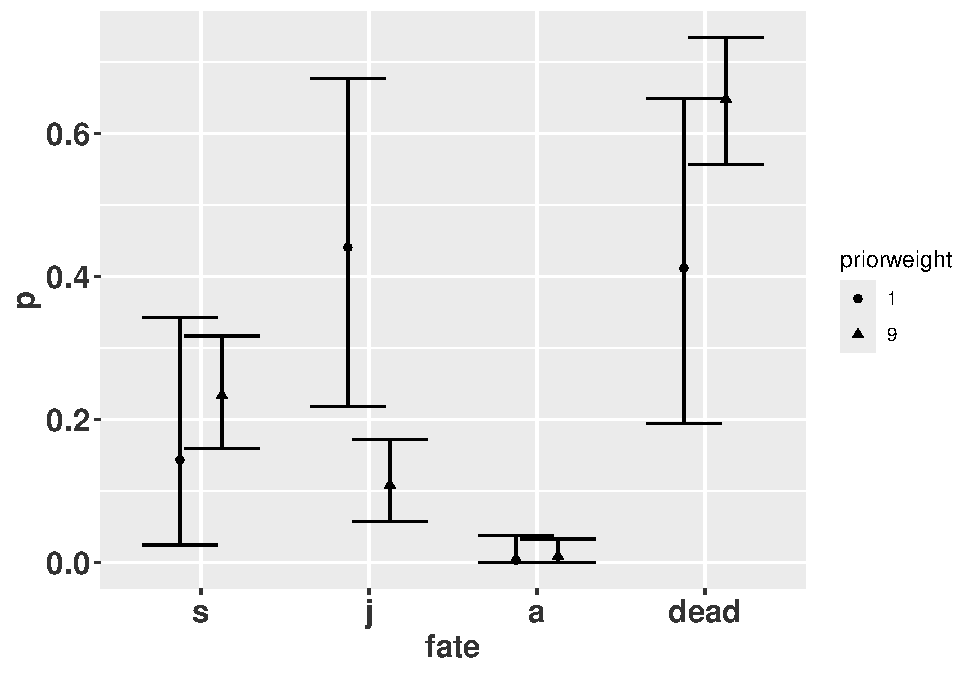
\includegraphics{Diagnostico_Poblacional_files/figure-latex/chap7_24-1.pdf}

La tasa de transición de plántula a juvenil se reduce cuando el tamaño de la muestra es demasiado grande. En general, el tamaño de la muestra previa debe ser menos que el tamaño de muestra observado.

\section{\texorpdfstring{Intervalos creíbles de \(\lambda\)}{Intervalos creíbles de \textbackslash lambda}}\label{intervalos-creuxedbles-de-lambda}

Obteniendo intervalos creíbles sobre la tasa de crecimiento asintótica, \(\lambda\), requiere simular matrices a partir de las distribuciones posteriores. Esto es algo complicado de hacer correctamente, y hemos escrito una función \texttt{raretrans::sim\_transitions()} para generar una lista de matrices simuladas dada la matriz observada y especificaciones previas.

\begin{Shaded}
\begin{Highlighting}[]
\FunctionTok{sim\_transitions}\NormalTok{(TF, N, }\AttributeTok{P =}\NormalTok{ RLT\_Tprior, }\AttributeTok{alpha =}\NormalTok{ alpha, }\AttributeTok{beta =}\NormalTok{ beta,}
                \AttributeTok{priorweight =} \FloatTok{0.5}\NormalTok{)}
\end{Highlighting}
\end{Shaded}

\begin{verbatim}
## [[1]]
##              [,1]        [,2]       [,3]
## [1,] 1.378969e-01 0.001807385 0.71113131
## [2,] 6.512527e-01 0.662296922 0.01054642
## [3,] 9.795676e-12 0.196184095 0.90243981
\end{verbatim}

Ahora simulamos 5000 veces, calculamos el valor \(\lambda\) de cada
matriz y creamos un histograma de la distribución.

\begin{Shaded}
\begin{Highlighting}[]
\CommentTok{\#set.seed(8390278) \# make this part reproducible}
\NormalTok{alpha2 }\OtherTok{\textless{}{-}} \FunctionTok{matrix}\NormalTok{(}\FunctionTok{c}\NormalTok{(}\ConstantTok{NA\_real\_}\NormalTok{, }\ConstantTok{NA\_real\_}\NormalTok{, }\FloatTok{0.025}\NormalTok{,}
                  \ConstantTok{NA\_real\_}\NormalTok{, }\ConstantTok{NA\_real\_}\NormalTok{, }\ConstantTok{NA\_real\_}\NormalTok{,}
                  \ConstantTok{NA\_real\_}\NormalTok{, }\ConstantTok{NA\_real\_}\NormalTok{, }\ConstantTok{NA\_real\_}\NormalTok{), }\AttributeTok{nrow=}\DecValTok{3}\NormalTok{, }\AttributeTok{ncol =} \DecValTok{3}\NormalTok{, }\AttributeTok{byrow =} \ConstantTok{TRUE}\NormalTok{)}
\NormalTok{beta2 }\OtherTok{\textless{}{-}} \FunctionTok{matrix}\NormalTok{(}\FunctionTok{c}\NormalTok{(}\ConstantTok{NA\_real\_}\NormalTok{, }\ConstantTok{NA\_real\_}\NormalTok{, }\DecValTok{1}\NormalTok{,}
                  \ConstantTok{NA\_real\_}\NormalTok{, }\ConstantTok{NA\_real\_}\NormalTok{, }\ConstantTok{NA\_real\_}\NormalTok{,}
                  \ConstantTok{NA\_real\_}\NormalTok{, }\ConstantTok{NA\_real\_}\NormalTok{, }\ConstantTok{NA\_real\_}\NormalTok{), }\AttributeTok{nrow=}\DecValTok{3}\NormalTok{, }\AttributeTok{ncol =} \DecValTok{3}\NormalTok{, }\AttributeTok{byrow =} \ConstantTok{TRUE}\NormalTok{)}
\CommentTok{\# generar 5000 matrices basado en las previas de transciones y de fertilidades, el tamaño de muestra, en adición de los datos}
\NormalTok{RLT\_0}\FloatTok{.5} \OtherTok{\textless{}{-}} \FunctionTok{sim\_transitions}\NormalTok{(TF, N, }\AttributeTok{P =}\NormalTok{ RLT\_Tprior, }\AttributeTok{alpha =}\NormalTok{ alpha2, }\AttributeTok{beta =}\NormalTok{ beta2,}
                \AttributeTok{priorweight =} \FloatTok{0.5}\NormalTok{, }\AttributeTok{samples =} \DecValTok{5000}\NormalTok{)}
\CommentTok{\# extract the lambdas for each matrix}
\NormalTok{RLT\_0}\FloatTok{.5} \OtherTok{\textless{}{-}} \FunctionTok{tibble}\NormalTok{(}\AttributeTok{lposterior =} \FunctionTok{map\_dbl}\NormalTok{(RLT\_0}\FloatTok{.5}\NormalTok{, lambda)) }\CommentTok{\# convertir la lista en un tibble}
\FunctionTok{ggplot}\NormalTok{(}\AttributeTok{data =}\NormalTok{ RLT\_0}\FloatTok{.5}\NormalTok{,}
       \AttributeTok{mapping =} \FunctionTok{aes}\NormalTok{(}\AttributeTok{x =}\NormalTok{ lposterior)) }\SpecialCharTok{+} 
  \FunctionTok{geom\_histogram}\NormalTok{(}\AttributeTok{binwidth =} \FloatTok{0.01}\NormalTok{, }\AttributeTok{colour=}\StringTok{"white"}\NormalTok{) }\SpecialCharTok{+} 
\NormalTok{  rlt\_theme}\SpecialCharTok{+} \FunctionTok{geom\_vline}\NormalTok{(}\AttributeTok{xintercept =} \DecValTok{1}\NormalTok{, }
                \AttributeTok{color =} \StringTok{"blue"}\NormalTok{, }\AttributeTok{size=}\FloatTok{1.5}\NormalTok{)}
\end{Highlighting}
\end{Shaded}

\begin{verbatim}
## Warning: Using `size` aesthetic for lines was deprecated in ggplot2 3.4.0.
## i Please use `linewidth` instead.
## This warning is displayed once every 8 hours.
## Call `lifecycle::last_lifecycle_warnings()` to see where this warning was
## generated.
\end{verbatim}

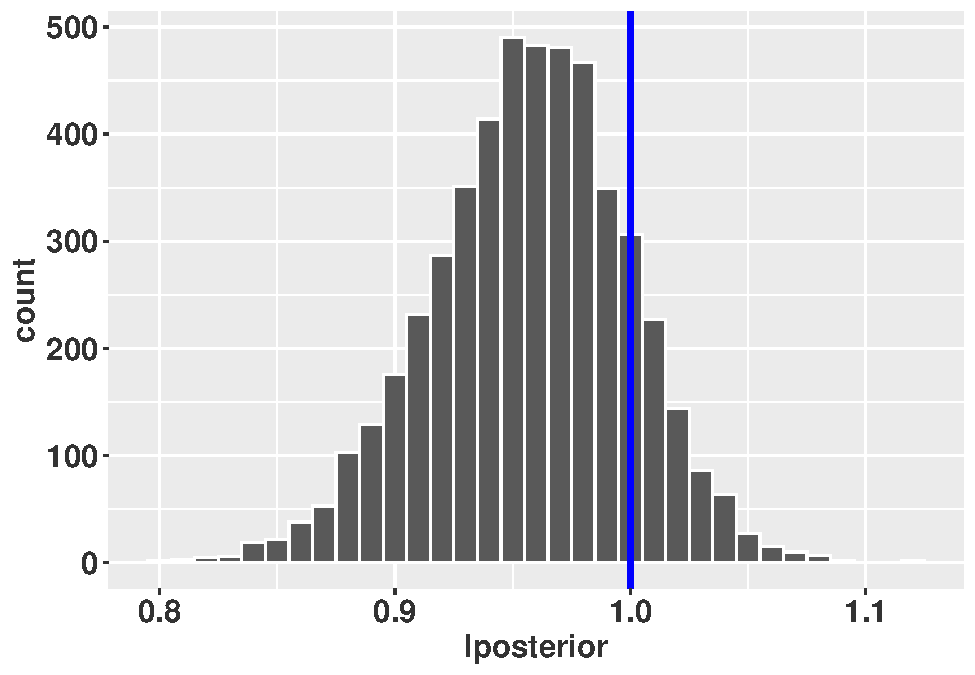
\includegraphics{Diagnostico_Poblacional_files/figure-latex/chap7_26-1.pdf}

\section{\texorpdfstring{Determinar si el \(\lambda\) es significativamente diferente de 1}{Determinar si el \textbackslash lambda es significativamente diferente de 1}}\label{determinar-si-el-lambda-es-significativamente-diferente-de-1}

Esa prueba es basada en la simulación de la distribución poesterior. Se calcula la distribución de los lambda's y se determina si el lmabda observado es significativamente más grande que 1.

También podemos calcular algunas estadísticas de resumen. \texttt{pincrease} es el
probabilidad de que \(\lambda > 1\).

\begin{Shaded}
\begin{Highlighting}[]
\NormalTok{RLT\_0}\FloatTok{.5}\NormalTok{\_summary }\OtherTok{\textless{}{-}} \FunctionTok{summarize}\NormalTok{(RLT\_0}\FloatTok{.5}\NormalTok{,}
                             \AttributeTok{medianL =} \FunctionTok{median}\NormalTok{(lposterior),}
                             \AttributeTok{meanL =} \FunctionTok{mean}\NormalTok{(lposterior),}
                             \AttributeTok{lcl =} \FunctionTok{quantile}\NormalTok{(lposterior, }\AttributeTok{probs =} \FloatTok{0.025}\NormalTok{),}
                             \AttributeTok{ucl =} \FunctionTok{quantile}\NormalTok{(lposterior, }\AttributeTok{probs =} \FloatTok{0.975}\NormalTok{),}
                             \AttributeTok{pincrease =} \FunctionTok{sum}\NormalTok{(lposterior }\SpecialCharTok{\textgreater{}} \FloatTok{1.}\NormalTok{)}\SpecialCharTok{/}\FunctionTok{n}\NormalTok{())}
\NormalTok{knitr}\SpecialCharTok{::}\FunctionTok{kable}\NormalTok{(RLT\_0}\FloatTok{.5}\NormalTok{\_summary, }\AttributeTok{digits =} \DecValTok{2}\NormalTok{)}
\end{Highlighting}
\end{Shaded}

\begin{tabular}{r|r|r|r|r}
\hline
medianL & meanL & lcl & ucl & pincrease\\
\hline
0.96 & 0.96 & 0.87 & 1.04 & 0.15\\
\hline
\end{tabular}

\}

\chapter{Crecimiento Poblacional}\label{crecimiento-poblacional}

Por: Tamara

\section{Introducción al crecimiento poblacional}\label{introducciuxf3n-al-crecimiento-poblacional}

Ahora el primer paso es explicar a que \ldots..

\begin{itemize}
\tightlist
\item
  Crecimiento intrínseco

  \begin{itemize}
  \tightlist
  \item
    Estimado de intervalos de confianza de lambda
  \end{itemize}
\end{itemize}

\section{Métodos}\label{muxe9todos}

\chapter{Estimación de Parametros}\label{estimaciuxf3n-de-parametros}

\section{Por: Mariana y Paola}\label{por-mariana-y-paola}

\section{En este capitulo se cubrirá varios estimación de parametros.}\label{en-este-capitulo-se-cubriruxe1-varios-estimaciuxf3n-de-parametros.}

\subsection{Condición basica de las matrices de transición}\label{condiciuxf3n-basica-de-las-matrices-de-transiciuxf3n}

\section{Librerías de R requeridas para el análisis}\label{libreruxedas-de-r-requeridas-para-el-anuxe1lisis}

\begin{Shaded}
\begin{Highlighting}[]
\FunctionTok{library}\NormalTok{(popdemo)}
\FunctionTok{library}\NormalTok{(popbio)}
\FunctionTok{library}\NormalTok{(ggplot2)}
\FunctionTok{library}\NormalTok{(dplyr)}
\FunctionTok{library}\NormalTok{(scales)}
\end{Highlighting}
\end{Shaded}

\begin{center}\rule{0.5\linewidth}{0.5pt}\end{center}

\begin{Shaded}
\begin{Highlighting}[]
\CommentTok{\#Capturar los datos de la matriz para L. rubripetala (Tremblay et al. 2015)}
\NormalTok{Lr1 }\OtherTok{\textless{}{-}} \FunctionTok{matrix}\NormalTok{(}\FunctionTok{c}\NormalTok{(}\FloatTok{0.4324}\NormalTok{, }\DecValTok{0}\NormalTok{,      }\DecValTok{0}\NormalTok{,     }\FloatTok{0.15}\NormalTok{,}
               \FloatTok{0.3784}\NormalTok{, }\FloatTok{0.8459}\NormalTok{, }\DecValTok{0}\NormalTok{,     }\DecValTok{0}\NormalTok{,}
               \DecValTok{0}\NormalTok{,      }\FloatTok{0.0034}\NormalTok{, }\FloatTok{0.7954}\NormalTok{,}\FloatTok{0.2300}\NormalTok{,}
               \DecValTok{0}\NormalTok{,      }\FloatTok{0.0890}\NormalTok{, }\FloatTok{0.1841}\NormalTok{,}\FloatTok{0.7510}\NormalTok{), }\AttributeTok{byrow=}\ConstantTok{TRUE}\NormalTok{,}\AttributeTok{ncol=}\DecValTok{4}\NormalTok{)}

\CommentTok{\#Capturar las categorias de estado}
\NormalTok{estadios }\OtherTok{\textless{}{-}} \FunctionTok{c}\NormalTok{(}\StringTok{"PL"}\NormalTok{, }\StringTok{"J"}\NormalTok{, }\StringTok{"NR"}\NormalTok{, }\StringTok{"AR"}\NormalTok{)}
\FunctionTok{colnames}\NormalTok{(Lr1) }\OtherTok{\textless{}{-}} \FunctionTok{rownames}\NormalTok{(Lr1) }\OtherTok{\textless{}{-}}\NormalTok{ estadios}

\CommentTok{\#Obtener la matriz L. rubripetala }
\NormalTok{Lr1 }\OtherTok{\textless{}{-}} \FunctionTok{matrix}\NormalTok{(Lr1[}\DecValTok{1}\SpecialCharTok{:}\DecValTok{4}\NormalTok{, ], }\AttributeTok{nrow =} \DecValTok{4}\NormalTok{, }\AttributeTok{dimnames =} \FunctionTok{list}\NormalTok{(estadios, estadios))}
\NormalTok{Lr1}
\end{Highlighting}
\end{Shaded}

\begin{verbatim}
##        PL      J     NR    AR
## PL 0.4324 0.0000 0.0000 0.150
## J  0.3784 0.8459 0.0000 0.000
## NR 0.0000 0.0034 0.7954 0.230
## AR 0.0000 0.0890 0.1841 0.751
\end{verbatim}

\emph{Paso 2: Comprobar que se cumplan los supuestos de la matriz de estudio}.

Previo al análisis de dinámica transitoria se debe comprobar que la matriz de transición poblacional sea: a) \emph{Cuadrada}, que tiene igual número de filas que de columnas, b) \emph{No negativa}, que todos sus elementos son positivos, por lo que son iguales o mayores a 0.000; c) \emph{Ergódica}, que el crecimiento asintótico es independiente de la estructura poblacional al inicio del estudio; d) \emph{Irreducible}, que los elementos de la matriz de análisis y, por lo tanto, los nodos de la gráfica del ciclo de vida, estén fuertemente conectados, tengan una ruta y desde cualquiera de las etapas pueda llegar a todas las otras formando un ciclo; e) \emph{Primitiva}, que el resultado de elevar a altas potencias una matriz irreducible positiva (i.e.~sin elementos negativos) único y tenga un sólo valor positivo (i.e.~tasa de crecimiento poblacional). Para más información sobre estas condiciones revisar: \citep{stott2010reducibility}.

Para evaluar si la matriz es cuadrada, no negativa, ergódica, primitiva e irreducible se usan las siguientes funciones de \emph{R}: \emph{dim}, \emph{isErgodic}, \emph{isPrimitive} y \emph{isIrreducible} respectivamente. A través del comando \emph{positiv} se determinó si todos los elementos de la matriz son positivos, por lo tanto, iguales o mayores a 0.000. A continuación se comprueba si la matriz de \emph{L. rubripetala} cumple con estas condiciones o supuestos.

\section{PASO 2: CONDICIONES QUE DEBE CUMPLIR LA MATRIZ DE ESTUDIO}\label{paso-2-condiciones-que-debe-cumplir-la-matriz-de-estudio}

\begin{Shaded}
\begin{Highlighting}[]
\CommentTok{\# a) Dimensión de la matriz (filas x columnas): los valores deben ser iguales}
\NormalTok{dimension }\OtherTok{\textless{}{-}} \FunctionTok{dim}\NormalTok{(Lr1)}

\CommentTok{\# b) No negativa }
\NormalTok{positiv }\OtherTok{\textless{}{-}} \FunctionTok{all}\NormalTok{(Lr1 }\SpecialCharTok{\textgreater{}=} \DecValTok{0}\NormalTok{)}

\CommentTok{\# c) Ergódica}
\NormalTok{ergodica }\OtherTok{\textless{}{-}} \FunctionTok{isErgodic}\NormalTok{(Lr1, }\AttributeTok{digits=}\DecValTok{5}\NormalTok{, }\AttributeTok{return.eigvec=}\ConstantTok{FALSE}\NormalTok{)}

\CommentTok{\# d) Irreducible}
\NormalTok{irreducible }\OtherTok{\textless{}{-}} \FunctionTok{isIrreducible}\NormalTok{(Lr1)}

\CommentTok{\# e) Primitiva}
\NormalTok{primitiva }\OtherTok{\textless{}{-}} \FunctionTok{isPrimitive}\NormalTok{(Lr1)}
\end{Highlighting}
\end{Shaded}

\begin{center}\rule{0.5\linewidth}{0.5pt}\end{center}

\emph{Paso 2a. Comprobación de los supuestos para las matrices de estudio}. En el siguiente cuadro se presentan los resultados que comprueban que la matriz de \emph{L. rubripetala} cumple con los supuestos establecidos para el análisis. Se comprueba que la matriz es cuadrada al tener 4 renglones y 4 columnas; asimismo, cumple con ser no negativa, ergódica, irreducible y primitiva al ser ``TRUE'' el resultado en los cuatro casos.

\begin{verbatim}
## [1] 4 4
\end{verbatim}

\begin{verbatim}
## [1] TRUE
\end{verbatim}

\begin{verbatim}
## [1] TRUE
\end{verbatim}

\begin{verbatim}
## [1] TRUE
\end{verbatim}

\begin{verbatim}
## [1] TRUE
\end{verbatim}

\begin{center}\rule{0.5\linewidth}{0.5pt}\end{center}

\emph{Paso 3: Análisis demográfico básico}.

En el análisis de dinámica transitoria necesitamos conocer cómo se comporta una población en el largo plazo, por lo que se proyecta el crecimiento poblacional de tipo asintótico para la matriz de la población seleccionada. Entonces, a partir de la matriz de proyección poblacional y el correspondiente vector de la estructura poblacional observada al inicio del estudio de \emph{L. rubripetala}, calcularemos la tasa de crecimiento poblacional (i.e.\emph{lambda}, de ahora en adelante \emph{lambda-max}), la estructura poblacional estable (\emph{w}, de ahora en adelante \emph{w-max}) y el valor reproductivo (\emph{v}), así como las matrices de sensibilidad y elasticidad. Con este fin, usaremos el procedimiento de la \emph{Sección X}, desarrollado en el programa \emph{popbio} de \emph{R}.

\begin{center}\rule{0.5\linewidth}{0.5pt}\end{center}

\subsection{Analisis de convergencia y ``Damping Ratio''}\label{analisis-de-convergencia-y-damping-ratio}

Además de esta información se estimarán dos nuevos indices: el tiempo de convergencia (\emph{convergence-time}) y el índice de amortiguamiento (\emph{damping-ratio}). El primero indica el tiempo esperado en que una población alcanza la estructura estable de una población con un crecimiento asimtótico, mientras que el segundo es una medida de que tan rápido (ciclos en tiempo de la matriz; meses, años) para que converge una población a la estructura estable (Caswell, 2001). Ese ultimo se calula dividiendo el valor propio dominante (el \emph{eigenvalue}) con el segundo valor dominante (la parte real), por consecuencia es una medida de cuan rápido la población regresa a su estructura poblacional estable despues de un disturbio, más grande el indice de \emph{damping ratio} más rapido converge a la estructura estable (\citet{stott2011framework}). Nota que el \emph{damping ratio} es un indice sin unidades y es independiente de la estructura original de la población (el vector de tamaño de muestra de cada etapa).

Los siguientes indices son una medida basado en el tiempo de las transiciones si bien, la mayoría de los datos de los estudios poblacionales han sido colectados para un periodo de tiempo anual (Crone et al.~2011), es importante recordar que algunos han sido colectados mensual, bimensulamente, por estación o de forma bianual, dependiendo del ciclo de vida de la especie de estudio. En el caso de \emph{L. rubripetala} los datos fueron colectados mensualmente, debido a la producción constante de estructuras reproductivas a lo largo del año \citep{tremblay2015stable}.

-- PASO 3: ANÁLISIS DEMOGRÁFICO BÁSICO: PROYECCIÓN DE LA POBLACIÓN --

\section{Análisis asintótico (i.e.~largo plazo) del crecimiento poblacional de L. rubripetala.}\label{anuxe1lisis-asintuxf3tico-i.e.-largo-plazo-del-crecimiento-poblacional-de-l.-rubripetala.}

\begin{Shaded}
\begin{Highlighting}[]
\CommentTok{\# PARÁMETROS POBLACIONALES}
\CommentTok{\# Tasa de crecimiento poblacional }
\NormalTok{lambda }\OtherTok{\textless{}{-}} \FunctionTok{lambda}\NormalTok{(Lr1)}

\CommentTok{\# Estructura estable de estados}
\NormalTok{Wmax }\OtherTok{\textless{}{-}} \FunctionTok{stable.stage}\NormalTok{(Lr1)}

\CommentTok{\# Valor reproductivo}
\NormalTok{v }\OtherTok{\textless{}{-}} \FunctionTok{reproductive.value}\NormalTok{(Lr1) }\CommentTok{\# Este no se habla en el texto}

\CommentTok{\# Matriz de elasticidad}
\NormalTok{elasticidad }\OtherTok{\textless{}{-}} \FunctionTok{round}\NormalTok{(}\FunctionTok{elas}\NormalTok{(Lr1), }\AttributeTok{digit =} \DecValTok{3}\NormalTok{)}

\CommentTok{\# Relación de amortiguamiento}
\NormalTok{dampingratio }\OtherTok{\textless{}{-}} \FunctionTok{dr}\NormalTok{(Lr1, }\AttributeTok{return.time =} \ConstantTok{TRUE}\NormalTok{, }\AttributeTok{x =} \DecValTok{10}\NormalTok{)}

\CommentTok{\# Tiempo de convergencia}
\NormalTok{n0 }\OtherTok{\textless{}{-}} \FunctionTok{c}\NormalTok{(}\DecValTok{0}\NormalTok{, }\DecValTok{46}\NormalTok{, }\DecValTok{38}\NormalTok{, }\DecValTok{82}\NormalTok{) }\CommentTok{\# la esturctura de la población inicial}
\NormalTok{tconvergencia }\OtherTok{\textless{}{-}} \FunctionTok{convt}\NormalTok{(Lr1, }\AttributeTok{accuracy =} \FloatTok{1e{-}3}\NormalTok{, }\AttributeTok{vector =}\NormalTok{ n0)}
\end{Highlighting}
\end{Shaded}

\begin{center}\rule{0.5\linewidth}{0.5pt}\end{center}

\subsubsection{Ergodicidad}\label{ergodicidad}

\subsubsection{Irreducible}\label{irreducible}

\subsubsection{Matriz Primitiva}\label{matriz-primitiva}

\begin{center}\rule{0.5\linewidth}{0.5pt}\end{center}

\section{Estructura estable}\label{estructura-estable}

La estructura estable de edades/etapas es un indice de la distribución proporcional de la poblacional que se espera que esta población alcance en el largo plazo. En el caso de \emph{Lepanthes rubripetala} se espera que la población alcance una estructura estable de 0.088, 0.206, 0.369 y 0.337 para las categorías de plántulas, juveniles, adultos no reproductivos y adultos reproductivos, respectivamente. Esta estructura asume que el crecimiento poblacional \emph{lambda} \(\lambda\) sigue igual y constante en el tiempo. Para una especie alcancar una estructura estable, el ambiente debería ser constante y sin cambios, lo cual es raramente el caso en la naturaleza. Esto asume que el periodo de muestreo y las condiciones abiotica y bioticas son tipica y constante. En un analisis de revisión de literatura Williams et al (\citet{williams2011distance}) encontraron que más del 80\% de las poblaciones no cumplia con la condición de estructura estable. En adición observarón que mayor desviación se obervaba en poblaciones con tiempo de generación largas y matriz grandes (n x n).

\begin{Shaded}
\begin{Highlighting}[]
\CommentTok{\#Estructura estable de estados}
\NormalTok{Wmax }\OtherTok{\textless{}{-}} \FunctionTok{stable.stage}\NormalTok{(Lr1)}
\NormalTok{Wmax}
\end{Highlighting}
\end{Shaded}

\begin{verbatim}
##         PL          J         NR         AR 
## 0.08789851 0.20619682 0.36907404 0.33683063
\end{verbatim}

Uno puede visualizar la estructura la estructura de la población usando el codigo siguiente.

\begin{Shaded}
\begin{Highlighting}[]
\NormalTok{Wdf}\OtherTok{=}\FunctionTok{data.frame}\NormalTok{(Wmax)}
\NormalTok{Wdf}\SpecialCharTok{$}\NormalTok{Categorias}\OtherTok{=}\FunctionTok{c}\NormalTok{(}\StringTok{"Plántulas"}\NormalTok{,}\StringTok{"Juveniles"}\NormalTok{,}\StringTok{"Adultos no reproductivos"}\NormalTok{,}\StringTok{"Adultos reproductivos"}\NormalTok{)}
\NormalTok{Wdf}\SpecialCharTok{$}\NormalTok{Categorias}\OtherTok{=}\FunctionTok{factor}\NormalTok{(Wdf}\SpecialCharTok{$}\NormalTok{Categorias, }\AttributeTok{levels=}\FunctionTok{c}\NormalTok{(}\StringTok{"Plántulas"}\NormalTok{,}\StringTok{"Juveniles"}\NormalTok{,}\StringTok{"Adultos no reproductivos"}\NormalTok{,}\StringTok{"Adultos reproductivos"}\NormalTok{))}
\FunctionTok{library}\NormalTok{(ggplot2)}

\FunctionTok{ggplot}\NormalTok{(Wdf, }\FunctionTok{aes}\NormalTok{(}\AttributeTok{y=}\NormalTok{Wmax, }\AttributeTok{x=}\NormalTok{Categorias)) }\SpecialCharTok{+} 
  \FunctionTok{geom\_bar}\NormalTok{(}\AttributeTok{stat=}\StringTok{"identity"}\NormalTok{, }\AttributeTok{fill=}\StringTok{"blue"}\NormalTok{) }\SpecialCharTok{+}
  \FunctionTok{labs}\NormalTok{(}\AttributeTok{title=}\StringTok{"Estructura estable de estados esperada"}\NormalTok{, }\AttributeTok{x=}\StringTok{"Etapas"}\NormalTok{, }\AttributeTok{y=}\StringTok{"Proporción"}\NormalTok{) }\SpecialCharTok{+}
  \FunctionTok{theme\_minimal}\NormalTok{()}
\end{Highlighting}
\end{Shaded}

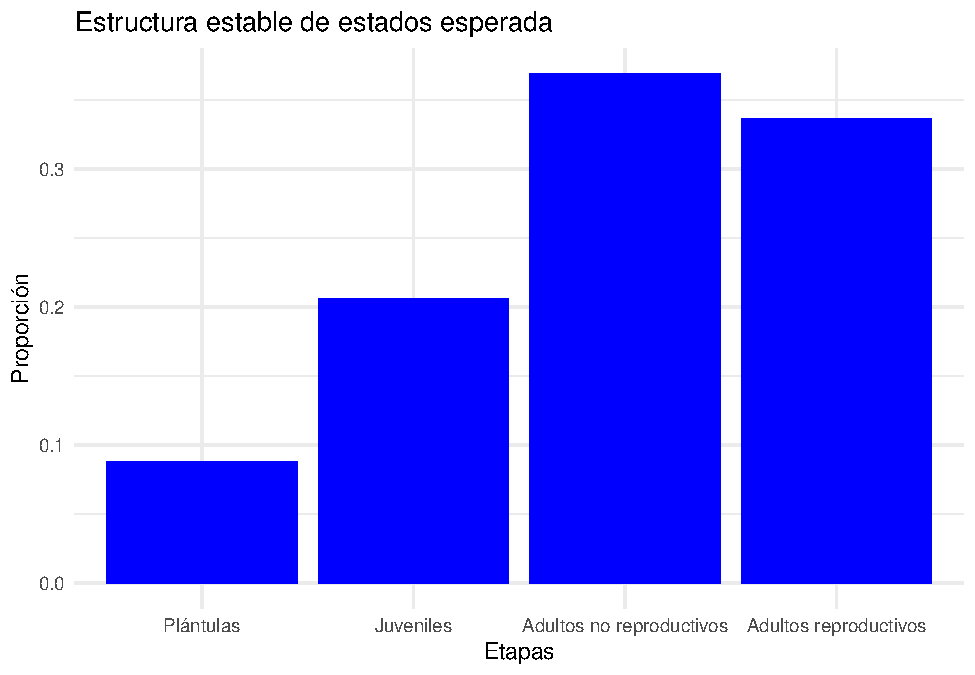
\includegraphics{Diagnostico_Poblacional_files/figure-latex/estructuraestable_viz-1.pdf}

\subsection{Damping Ratio}\label{damping-ratio}

\section{Análisis de Amortiguamiento/Damping Ratio}\label{anuxe1lisis-de-amortiguamientodamping-ratio}

El análisis de amortiguamiento es un indice de la rapidez con la que una población converge a su estructura estable después de un disturbio \citep{jiang2020life}. El indice de amortiguamiento \(d > 0\), y más grande el indice de amortiguamiento más rápido la población converge a la estructura estable. Se ha demostrado que hay una relación entre el indice de amortiguamiento y tiempo de generación de una especie \citep{jiang2020life}. El tiempo de amortiguamiento se calcula \(\tau=1/d\). Usando la función \emph{dr} del paquete \textbf{popbio}, en el caso de \emph{Lepanthes rubripetala} se espera estima que el indice de amortigamiento es 1.2 y que la población converga a su estructura estable en 12 meses, ya que los datos fueron recolectado y analizado mensualmente. Si los datos hubiese sido recolectado una vez al año entonces la población converga a su estructura estable en 12 años. Un supuesto importante es que la tasa de crecimiento intrínseca es igual para todos los periodos subsiguientes.

\begin{Shaded}
\begin{Highlighting}[]
\CommentTok{\#Relación de amortiguamiento}
\NormalTok{dampingratio }\OtherTok{\textless{}{-}} \FunctionTok{dr}\NormalTok{(Lr1, }\AttributeTok{return.time=}\ConstantTok{TRUE}\NormalTok{)}
\NormalTok{dampingratio}
\end{Highlighting}
\end{Shaded}

\begin{verbatim}
## $dr
## [1] 1.210702
## 
## $t
## [1] 12.04278
\end{verbatim}

\begin{center}\rule{0.5\linewidth}{0.5pt}\end{center}

\section{Análisis de Convergencia}\label{anuxe1lisis-de-convergencia}

El tiempo de convergencia puede ser calculado a base de la cantidad de individuos en las diferentes etapas o edades. El tiempo de convergencia es el tiempo esperado en que una población alcanza la estructura estable. En el caso de \emph{Lepanthes rubripetala} se espera que la población alcance la estructura estable en 25 meses si se comienza con una población sesgada de solamente plántulas (n=1000) y ninguno en las etapas subsiguientes.

\begin{Shaded}
\begin{Highlighting}[]
\CommentTok{\# Tiempo de convergencia}
\NormalTok{n }\OtherTok{=} \FunctionTok{c}\NormalTok{(}\DecValTok{1000}\NormalTok{, }\DecValTok{0}\NormalTok{, }\DecValTok{0}\NormalTok{, }\DecValTok{0}\NormalTok{)}
\NormalTok{tconvergencia }\OtherTok{\textless{}{-}} \FunctionTok{convt}\NormalTok{(Lr1, }\AttributeTok{accuracy =} \FloatTok{1e{-}3}\NormalTok{, }\AttributeTok{vector =}\NormalTok{ n)}
\NormalTok{tconvergencia}
\end{Highlighting}
\end{Shaded}

\begin{verbatim}
## [1] 25
\end{verbatim}

Si comenzamos con una población mucho más cerca a la estructura estable, podemos calcular el tiempo de convergencia. Digamos que se comienza con una población de 8, 20, 27 34 individuos en las etapas plantulas, juveniles, adultos no reproductivos y adultos reproductivos, respectivamente. En este caso se espera que la población alcance la estructura estable en 6 meses. En este caso vemos que el tiempo de convergencia es mucho más corto que si se comienza con una población sesgada de solamente plántulas. Es acercamiento puede ser util cuando se hace trabajo de conservación, por ejemplo se establece una nueva población con x cantidades de individuos en cada etapa.

\begin{Shaded}
\begin{Highlighting}[]
\NormalTok{n2 }\OtherTok{=} \FunctionTok{c}\NormalTok{(}\DecValTok{8}\NormalTok{, }\DecValTok{20}\NormalTok{, }\DecValTok{27}\NormalTok{, }\DecValTok{34}\NormalTok{)}
\NormalTok{tconvergencia }\OtherTok{\textless{}{-}} \FunctionTok{convt}\NormalTok{(Lr1, }\AttributeTok{accuracy =} \FloatTok{1e{-}3}\NormalTok{, }\AttributeTok{vector =}\NormalTok{ n2)}
\NormalTok{tconvergencia}
\end{Highlighting}
\end{Shaded}

\begin{verbatim}
## [1] 6
\end{verbatim}

\begin{center}\rule{0.5\linewidth}{0.5pt}\end{center}

\section{Valores reproductivos}\label{valores-reproductivos}

El valor reproductivo \emph{v} es un indice de la contribución de cada categoría de edad/estado a la tasa de crecimiento poblacional. En el caso de \emph{Lepanthes rubripetala} se espera que la categoría de adultos reproductivos contribuya más a la tasa de crecimiento poblacional, seguido por la categoría de adultos no reproductivos, juveniles y plántulas. Los valores en la lista de \emph{v} se compara con la primera edad/estado y siempre la primera etapa/estado tiene un valor de 1.000. Por consecuencia un individuo de la 4ta etapa (adulto reproductivo) tiene un potencial de dejar 2.7 individuos al comparar que una plantula tiene solamente tiene un valor de 1.0. La diferencia es que los individuos pequeños tienen que sobrevivir y llegar a las etapas mayores para contribuir a la tasa de crecimiento poblacional.

\begin{Shaded}
\begin{Highlighting}[]
\NormalTok{valor\_repro}\OtherTok{=}\FunctionTok{reproductive.value}\NormalTok{(Lr1)}
\NormalTok{valor\_repro}
\end{Highlighting}
\end{Shaded}

\begin{verbatim}
##       PL        J       NR       AR 
## 1.000000 1.519043 2.316113 2.664676
\end{verbatim}

\chapter{Elasticidad}\label{elasticidad}

Autores: ``Mariana Hernández Apolinar y Paola Portillo Tzompa''

\section{Qué es la Elasticidad}\label{quuxe9-es-la-elasticidad}

El concepto de elasticidad en biología es un método orientado a evaluar el cambio proporcional en una variable en respuesta a un cambio proporcional en otra variable. En términos de matrices de transición, la elasticidad es una medida de la sensibilidad de la tasa de crecimiento poblacional a cambios. En otra palabra si uno cambia uno de los parámetros de la matriz de transición, la elasticidad mide cuánto cambiaria la tasa de crecimiento poblacional (ref). En biología, la elasticidad es una herramienta es para entender la importancia de cada etapa de la historia de vida sobre la tasa de crecimiento poblacional ya que permite identificar las etapas que más contribuyen a la tasa de crecimiento poblacional con menor cambios. Esa herramienta es muy útil para la conservación de especies y para la gestión de recursos naturales por que en parte nos indica cuan sensitiva esta el crecimento poblacional cuando se cambia los parámetros de la historia de vida (las transiciones, supervivencia y fecundidad) de una especie

El concepto de elasticidad se puede aplicar en muchas diferentes áreas, tanto biológicos, matemáticos, estudios sociales, financieros y económicos (ref). Por ejemplo en economía Alfred Marshall fue uno de los primeros en usar el concepto de elasticidad para entender la relación entre la oferta y la demanda de un producto donde el uso el termino de ``responsiveness'' para describir la elasticidad en el libro \emph{The Economics of Industry} publicado en 1879. En biología un ejemplo clásico de elasticidad \ldots.

\section{Librerías de R requeridas para el análisis}\label{libreruxedas-de-r-requeridas-para-el-anuxe1lisis-1}

\begin{Shaded}
\begin{Highlighting}[]
\FunctionTok{library}\NormalTok{(popdemo)}
\FunctionTok{library}\NormalTok{(popbio)}
\FunctionTok{library}\NormalTok{(ggplot2)}
\FunctionTok{library}\NormalTok{(dplyr)}
\FunctionTok{library}\NormalTok{(scales)}
\end{Highlighting}
\end{Shaded}

\begin{center}\rule{0.5\linewidth}{0.5pt}\end{center}

\begin{Shaded}
\begin{Highlighting}[]
\CommentTok{\#Capturar los datos de la matriz para L. rubripetala (Tremblay et al. 2015)}
\NormalTok{Lr1 }\OtherTok{\textless{}{-}} \FunctionTok{matrix}\NormalTok{(}\FunctionTok{c}\NormalTok{(}\FloatTok{0.4324}\NormalTok{, }\DecValTok{0}\NormalTok{,      }\DecValTok{0}\NormalTok{,     }\FloatTok{0.15}\NormalTok{,}
               \FloatTok{0.3784}\NormalTok{, }\FloatTok{0.8459}\NormalTok{, }\DecValTok{0}\NormalTok{,     }\DecValTok{0}\NormalTok{,}
               \DecValTok{0}\NormalTok{,      }\FloatTok{0.0034}\NormalTok{, }\FloatTok{0.7954}\NormalTok{,}\FloatTok{0.2300}\NormalTok{,}
               \DecValTok{0}\NormalTok{,      }\FloatTok{0.0890}\NormalTok{, }\FloatTok{0.1841}\NormalTok{,}\FloatTok{0.7510}\NormalTok{), }\AttributeTok{byrow=}\ConstantTok{TRUE}\NormalTok{,}\AttributeTok{ncol=}\DecValTok{4}\NormalTok{)}

\CommentTok{\#Capturar las categorias de estado}
\NormalTok{estadios }\OtherTok{\textless{}{-}} \FunctionTok{c}\NormalTok{(}\StringTok{"PL"}\NormalTok{, }\StringTok{"J"}\NormalTok{, }\StringTok{"NR"}\NormalTok{, }\StringTok{"AR"}\NormalTok{)}
\FunctionTok{colnames}\NormalTok{(Lr1) }\OtherTok{\textless{}{-}} \FunctionTok{rownames}\NormalTok{(Lr1) }\OtherTok{\textless{}{-}}\NormalTok{ estadios}

\CommentTok{\#Obtener la matriz L. rubripetala }
\NormalTok{Lr1 }\OtherTok{\textless{}{-}} \FunctionTok{matrix}\NormalTok{(Lr1[}\DecValTok{1}\SpecialCharTok{:}\DecValTok{4}\NormalTok{, ], }\AttributeTok{nrow =} \DecValTok{4}\NormalTok{, }\AttributeTok{dimnames =} \FunctionTok{list}\NormalTok{(estadios, estadios))}
\NormalTok{Lr1}
\end{Highlighting}
\end{Shaded}

\begin{verbatim}
##        PL      J     NR    AR
## PL 0.4324 0.0000 0.0000 0.150
## J  0.3784 0.8459 0.0000 0.000
## NR 0.0000 0.0034 0.7954 0.230
## AR 0.0000 0.0890 0.1841 0.751
\end{verbatim}

\section{Cómo se interpreta la elasticidad}\label{cuxf3mo-se-interpreta-la-elasticidad}

\section{Cómo se calcula la elasticidad}\label{cuxf3mo-se-calcula-la-elasticidad}

\begin{center}\rule{0.5\linewidth}{0.5pt}\end{center}

\section{Análisis de elasticidad}\label{anuxe1lisis-de-elasticidad}

La elasticidad es un indice de la sensibilidad de la tasa de crecimiento poblacional a los cambios en las tasas de supervivencia, crecimiento y reproducción de cada categoría de edad/estado. La suma de todas las proporciones es 1.0, por consecuencia uno puede comparar el efecto de cambios proporcional en cada parámetro y evaluar su impacto. En el caso de \emph{Lepanthes rubripetala} se espera que la tasa de crecimiento poblacional sea más sensible a los cambios en la supervivencia de los etapas 3 y 4 ya que tienen una elasticidad de 0.313 y 0.311 respectivamente. Si sumamos el componente de supervivencia (la diagonal) de la matriz de transición poblacional, la suma es (0.018 + 0.122 + 0.313 + 0.311) = 0.764. Por consecuencia, las etapas de supervivencia de los individuos contribuyen a 76.4\% y son las etapas más sensitivas a los cambios demográficos. Al comparar si uno fuese a hacer un cambio proporcional en la reproducción (los adultos que dejan plántulas) tendría un impacto mucho más pequeño, solamente de 2.3\%.

Los análisis de elasticidad pueden ser usado para evaluar que etapas que pudiese ayudar en enfocar las alternativas de manejo para cambiar la tasa de crecimiento poblacional. Por ejemplo si es una especie en peligro de extinción, uno puede enfocar los trabajos de manejo de la especie en mejorar la supervivencia de los individuos de las etapas más sensitivas. Al contrario si es una especie invasora, uno puede enfocar los trabajos de manejo en reducir la supervivencia de las etapas más sensitivas. En este caso seria reducir la supervivencia de los adultos reproductivos y no reproductivos. Enfocando en las etapas más sensitivas es una forma de maximizar el impacto de los trabajos de manejo con menos recursos. Naturalmente se asume que el manejo de estas etapas es posible, por ejemplo si la elasticidad es alta en una de las tranciciones, por ejemplo juvenil a adultos, pero no se conoce cual son la variables ambientales que impacta esa transiciones no se puede hacer un manejo efectivo.

\begin{Shaded}
\begin{Highlighting}[]
\CommentTok{\#Matriz de elasticidad}
\NormalTok{elasticidad }\OtherTok{\textless{}{-}} \FunctionTok{round}\NormalTok{(}\FunctionTok{elas}\NormalTok{(Lr1),}\AttributeTok{digit=}\DecValTok{3}\NormalTok{)}
\NormalTok{elasticidad}
\end{Highlighting}
\end{Shaded}

\begin{verbatim}
##       PL     J    NR    AR
## PL 0.018 0.000 0.000 0.023
## J  0.023 0.122 0.000 0.000
## NR 0.000 0.001 0.313 0.083
## AR 0.000 0.023 0.083 0.311
\end{verbatim}

\section{Limitaciones}\label{limitaciones}

\chapter{Dinámica transitoria (Transient dynamics)}\label{dinuxe1mica-transitoria-transient-dynamics}

Autores: ``Mariana Hernández Apolinar y Paola Portillo Tzompa''

\section{Dinámica poblacional de largo y corto plazo}\label{dinuxe1mica-poblacional-de-largo-y-corto-plazo}

Los modelos de proyección poblacional (MPP), previamente vistos en la \emph{Sección XX}, son los más utilizados para proyectar la razón de crecimiento de una población después de varios años (i.e.~largo plazo) asumiendo que la razón de muertes, la reproducción y el crecimiento de los individuos en las distintas categorías de la población (i.e.~tasas vitales) no varían en el tiempo debido a la presencia de condiciones ambientales constantes (Caswell, 2001; Crone et al.~2011; Koons et al.~2021). Al mantenerse constantes estas variables en el largo plazo (i.e.~deterministas), la población incrementará o decrecerá a una velocidad constante y no cambiará la proporción de individuos por categoría de tamaño/estado (i.e.~comportamiento asintótico), {[}\citet{bierzychudek1999looking}; Caswell, 2001). Sin embargo, en la naturaleza estas variables distan de ser constantes (i.e.~deterministas), debido a que las poblaciones experimentan recursos limitados (v.g. alimento, sitios de refugio), ambientes heterogéneos y cambiantes que perturban las poblaciones (v.g. deforestación, sequía, huracanes, enfermedades, etc), afectando su dinámica y sugiriendo que la tasa de crecimiento de largo plazo no es un buen predictor de los cambios que enfrentan dichas las poblaciones (\citet{bierzychudek1999looking}). De ahí que, se hayan desarrollado modelos que integran dicha variación y que permiten hacer proyecciones más realistas sobre la dinámica poblacional de la especie de estudio, tal es el caso de los modelos de crecimiento estocástico y los análisis de dinámica transitoria.

En particular, los modelos de dinámica transitoria surgen como una alternativa para analizar la dinámica de una población en el corto plazo, cuando se presenta un evento de perturbación repentino que afecta la abundancia de individuos en una o varias de las categorías de poblacional (i.e.cambios en el modelo) o que la estructura de la población varia en tiempo. El analisis no asume cambios en las entradas de la matriz de transición (i.e.~condiciones constantes; Vindeness et al.~2021). De esta forma, en este análisis se evalúa la respuesta inmediata de la población; es decir, antes de alcanzar la estructura estable de estadios/edades y de crecer a una tasa constante (Bierzichudek, 1999; Koons et al.~2021, Stott et al.~2010). Esta respuesta de corto plazo es pasajera o temporal y resulta de suponer que la estructura inicial de la población es inestable; de ahí, el nombre de ``dinámica transitoria''. Bajo este supuesto, es importante saber qué tanto influye dicha estructura inicial inestable en la dinámica poblacional temporal de corto plazo (Koon et al.~2021). Esta respuesta se determina a través de las discrepancias o diferencias que hay entre la estructura inicial (i.e.~corto plazo) y la estructura estable (i.e.~largo plazo) de la población analizada \citep{raventos2015transient}.

A partir de lo anterior, es evidente que los dos acercamiento para evaluar la dinamica poblacional usando el método tradicional o de de dinámica transitoria abordan distintos aspectos de la dinámica poblacional de una especie y, por lo tanto, hacen uso de ecuaciones distintas en su análisis (Koons et al.~2021). A continuación se listan la serie de pasos a seguir para facilitar y asimilar el desarrollo del complejo análisis de la dinámica transitoria. Este análisis fue planteado por Stott y colaboradores \citep{stott2011framework, stott2012beyond, stott2012popdemo} y se lleva a cabo en el Programa de estadística \emph{R}.

***

\emph{Paso 1. Matriz de transición y estructura poblacional inicial}.

En primer lugar se debe contar con una matriz de proyección poblacional y su correspondiente vector de la estructura poblacional observada al inicio del estudio. A lo largo del desarrollo del análisis en el presente Capítulo se usarán los datos obtenidos por Tremblay et al. \citep{tremblay2015stable} y Schödelbauerová et al. \citep{schodelbauerova2010prediction} para la orquídea epífita \emph{Lepanthes rubripetala}; en específico usaremos los datos de la población 1. En esta especie, los individuos se clasificaron en cuatro categorías de estado: plántula (PL), juvenil (J), adulto no reproductivo (NR) y adulto reproductivo (AR). Esta última catergoría florece a largo de todo el año, por lo que el seguimiento de la población fue mensual \citep{tremblay2015stable, schodelbauerova2010prediction}.

En primer lugar se debe contar con una matriz de proyección poblacional y su vector correspondiente de la estructura poblacional observada al inicio del estudio. En en este caso se usarán los datos obtenidos para \emph{Lepanthes rubripetala} por Tremblay y colaboradores \citep{tremblay2015stable, schodelbauerova2010prediction}.

A continuación incorporamos la información de nuestra matriz y la abundancia de individuos por categoría observada al inicio de nuestro estudio. Las función \emph{matrix} de \emph{R} fue usada para construir la matriz y \emph{n0} se fue usado para nombrar el vector de la estructura inicial obsevada. Cabe señalar que se, a lo largo del análisis de dinámica transitoria se usan cinco paquetes de \emph{R} (\emph{popdemo}, \emph{popbio}, \emph{ggplot2}, \emph{dplyr}, \emph{scales}), por lo que se cargan desde un principio.

\begin{center}\rule{0.5\linewidth}{0.5pt}\end{center}

\section{PROYECTO DE DINAMICA TRANSITORIA O DE CORTO PLAZO}\label{proyecto-de-dinamica-transitoria-o-de-corto-plazo}

\subsection{PART I: DINÁMICA POBLACIONAL DE LARGO PLAZO}\label{part-i-dinuxe1mica-poblacional-de-largo-plazo}

Éste es un análisis de dinámica transitoria para \emph{Lepanthes rubripetala} (Población 1), cuyo ciclo de vida fue dividido en cuatro clases de estado:

\begin{itemize}
\tightlist
\item
  PL = plántula,
\item
  J = juvenil,
\item
  NR = adultos no reproductivos,
\item
  AR = adultos reproductivos.
\end{itemize}

\begin{center}\rule{0.5\linewidth}{0.5pt}\end{center}

\section{Librerías de R requeridas para el análisis}\label{libreruxedas-de-r-requeridas-para-el-anuxe1lisis-2}

\begin{Shaded}
\begin{Highlighting}[]
\FunctionTok{library}\NormalTok{(popdemo)}
\FunctionTok{library}\NormalTok{(popbio)}
\FunctionTok{library}\NormalTok{(ggplot2)}
\FunctionTok{library}\NormalTok{(dplyr)}
\FunctionTok{library}\NormalTok{(scales)}
\end{Highlighting}
\end{Shaded}

\begin{center}\rule{0.5\linewidth}{0.5pt}\end{center}

\subsection{\texorpdfstring{PASO 1. MATRIZ DE PROYECCIÓN POBLACIONAL y ESTRUCTURA POBLACIONAL INICIAL \(t_{0}\)}{PASO 1. MATRIZ DE PROYECCIÓN POBLACIONAL y ESTRUCTURA POBLACIONAL INICIAL t\_\{0\}}}\label{paso-1.-matriz-de-proyecciuxf3n-poblacional-y-estructura-poblacional-inicial-t_0}

\begin{Shaded}
\begin{Highlighting}[]
\CommentTok{\#Capturar los datos de la matriz para L. rubripetala (Tremblay et al. 2015)}
\NormalTok{Lr1 }\OtherTok{\textless{}{-}} \FunctionTok{matrix}\NormalTok{(}\FunctionTok{c}\NormalTok{(}\FloatTok{0.4324}\NormalTok{, }\DecValTok{0}\NormalTok{,      }\DecValTok{0}\NormalTok{,     }\FloatTok{0.15}\NormalTok{,}
               \FloatTok{0.3784}\NormalTok{, }\FloatTok{0.8459}\NormalTok{, }\DecValTok{0}\NormalTok{,     }\DecValTok{0}\NormalTok{,}
               \DecValTok{0}\NormalTok{,      }\FloatTok{0.0034}\NormalTok{, }\FloatTok{0.7954}\NormalTok{,}\FloatTok{0.2300}\NormalTok{,}
               \DecValTok{0}\NormalTok{,      }\FloatTok{0.0890}\NormalTok{, }\FloatTok{0.1841}\NormalTok{,}\FloatTok{0.7510}\NormalTok{), }\AttributeTok{byrow=}\ConstantTok{TRUE}\NormalTok{,}\AttributeTok{ncol=}\DecValTok{4}\NormalTok{)}

\CommentTok{\#Capturar las categorias de estado}
\NormalTok{estadios }\OtherTok{\textless{}{-}} \FunctionTok{c}\NormalTok{(}\StringTok{"PL"}\NormalTok{, }\StringTok{"J"}\NormalTok{, }\StringTok{"NR"}\NormalTok{, }\StringTok{"AR"}\NormalTok{)}
\FunctionTok{colnames}\NormalTok{(Lr1) }\OtherTok{\textless{}{-}} \FunctionTok{rownames}\NormalTok{(Lr1) }\OtherTok{\textless{}{-}}\NormalTok{ estadios}

\CommentTok{\#Obtener la matriz L. rubripetala }
\NormalTok{Lr1 }\OtherTok{\textless{}{-}} \FunctionTok{matrix}\NormalTok{(Lr1[}\DecValTok{1}\SpecialCharTok{:}\DecValTok{4}\NormalTok{, ], }\AttributeTok{nrow =} \DecValTok{4}\NormalTok{, }\AttributeTok{dimnames =} \FunctionTok{list}\NormalTok{(estadios, estadios))}
\NormalTok{Lr1}
\end{Highlighting}
\end{Shaded}

\begin{verbatim}
##        PL      J     NR    AR
## PL 0.4324 0.0000 0.0000 0.150
## J  0.3784 0.8459 0.0000 0.000
## NR 0.0000 0.0034 0.7954 0.230
## AR 0.0000 0.0890 0.1841 0.751
\end{verbatim}

\begin{Shaded}
\begin{Highlighting}[]
\CommentTok{\# Capturar y obtener el vector inicial (datos de campo) de clases de estado población 1 (Schödelbauerová et al. 2010)}

\NormalTok{n0 }\OtherTok{\textless{}{-}} \FunctionTok{c}\NormalTok{(}\DecValTok{0}\NormalTok{, }\DecValTok{46}\NormalTok{, }\DecValTok{38}\NormalTok{, }\DecValTok{82}\NormalTok{) }
\NormalTok{n0}
\end{Highlighting}
\end{Shaded}

\begin{verbatim}
## [1]  0 46 38 82
\end{verbatim}

***

\subsubsection{Capturar y obtener el vector inicial (datos de campo) de clases de estado población 1}\label{capturar-y-obtener-el-vector-inicial-datos-de-campo-de-clases-de-estado-poblaciuxf3n-1}

\emph{Paso 1a. Matriz de transición y estructura poblacional inicial}. En el siguiente cuadro se comprueba que la matriz de la estructura poblacional inicial de \emph{L. rubripetala} haya sido incorporada sin errores. La primera formada por 4 renglones y 4 columnas y la segunda por 4 elementos, que indican el número de individuos encontrados en el estado de plántula (0), juvenil (46), adulto no reproductivo (38) y adulto reproductivo (82) \citep{tremblay2015stable, schodelbauerova2010prediction}.

\begin{verbatim}
##        PL      J     NR    AR
## PL 0.4324 0.0000 0.0000 0.150
## J  0.3784 0.8459 0.0000 0.000
## NR 0.0000 0.0034 0.7954 0.230
## AR 0.0000 0.0890 0.1841 0.751
\end{verbatim}

\begin{verbatim}
## [1]  0 46 38 82
\end{verbatim}

***

\subsection{Crecimiento asintótico}\label{crecimiento-asintuxf3tico}

La definición del crecimiento asintótico de la población \emph{lambda} se basa en la tasa de crecimiento poblacional cuando la población este a su nivel estable de estructura de edades/estados. Por consecuencia se asume que la población llegue o este a un nivel estructura de edades/estados estable. Para la población de \emph{Lepanthes rubripetala} se obtiene una tasa de crecimiento poblacional de 1.007, lo que indica que la población crece a una tasa constante de 1.007 entre \(t_{0}\) y \(t_{1}\). Entonces si la población tuviese 1000 individuos en promedio hubiese 7 individuos más en \(t_{1}\) o sea el siguiente mes. Nota que las poblaciones de \emph{Lepanthes} nunca son tan grandes (\citet{tremblay1997distribution}), pero es un ejemplo para ilustrar el concepto.

\begin{Shaded}
\begin{Highlighting}[]
\CommentTok{\#Análisis asintótico (i.e. largo plazo) del crecimiento poblacional de L. rubripetala}
\CommentTok{\#La orquídea florece todo el año, por lo que el seguimiento de la población fue mensual. }

\CommentTok{\#PARÁMETROS POBLACIONALES}
\DocumentationTok{\#\#lambda: Tasa de crecimiento poblacional}


\NormalTok{lambda }\OtherTok{\textless{}{-}}\FunctionTok{lambda}\NormalTok{(Lr1)}
\NormalTok{lambda}
\end{Highlighting}
\end{Shaded}

\begin{verbatim}
## [1] 1.007206
\end{verbatim}

\section{Dinámica transitoria}\label{dinuxe1mica-transitoria}

En la dinámica transitoria o de corto plazo, Stott y colaboradores (2010, 2012) incorporaron la estocasticidad demográfica para analizar el cambio de la estructura poblacional debido a una perturbación de origen biótico, abiótico o antropogénico (i.e.~cambios en la estructura incicial observada). Este tipo de estocasticidad se refiere a la sobrevivencia y reproducción en número entero y finito; es decir, un individuo sobrevive o no, lo cual se representa con 1 ó 0, al igual que puede reproducirse (1) o no (0). La incorporación de esta característica en los individuos genera una variación no cíclica ni predecible en la respuesta de los individuos de una población.

En el análisis transitorio, el modelo sesgado por etapas (i.e.~categorías) es el procedimiento que se usa para evaluar la perturbación de la estructura inicial. La perturbación o sesgo en la estructura inicial se evalúa modificando la proporción de individuos presentes en alguna categoría de la estructura poblacional. Cabe señalar que estas modificaciones representan distintos escenarios o simulaciones que ocurren o pueden ocurrir en nuestra población de estudio.

Por ejemplo, la estructura inicial en la población 1 de \emph{Lepanthes rubripetala} fue la siguiente: (0,46,38,82). En este caso, al modificar la proporción de individuos presente en una, dos o en todas las categorías de la población se simuló el cambio en la dinámica en el corto plazo; es decir, en un momento previo a que se alcance el crecimiento estable o de largo plazo. En \emph{Lepanthes rubripetala} se hicieron cinco simulaciones o escenarios al suponer las siguientes proporciones de individuos por categoría (Tremblay et al, 2015):

\begin{enumerate}
\def\labelenumi{\arabic{enumi}.}
\tightlist
\item
  Límite inferior: (1,0,0,0), los individuos de la población se contran en la categoría de plántulas (Lower bound).
\item
  Inicio I: (0.15, 0.35, 0,30, 0.20), mayor proporción de individuos en las categorías juvenil y adulto no reproductivo.
\item
  Estructura estable de la población: los individuos de la población tienen una abundancia de acuerdo con \emph{w-max}.
\item
  Inicio II: (0.4, 0.2,0.2, 0.2), mayor proporción de plántulas y una proporción similar en las categorías juvenil, adulto no reproductivo y adulto reproductivo.
\item
  Límite superior: (0,0,0,1), los individuos de la población se contran en la categoría de adulto reproductivo.
\end{enumerate}

\emph{Dinámica poblacional absoluta}. Como consecuencia de las perturbaciones o escenarios existen cambios en el crecimiento poblacional, los cuales son evidentes si se grafican. Un aspecto a considerar es que, la gráfica que se genera incluye la influencia de la dinámica trasitoria y asintótica, por lo que se le denomina dinámica poblacional absoluta (Fig. 2A de Tremblay y colaboradores, 2015).

\begin{Shaded}
\begin{Highlighting}[]
\DocumentationTok{\#\#PASO 4. DINÁMICA POBLACIONAL ABSOLUTA.    }
\CommentTok{\#Se proyecta el crecimiento poblacional ante cambios en la estructura }
\CommentTok{\#inicial debidos a la perturbación (5 escenarios). Esta gráfica incluye la }
\CommentTok{\#influencia de la dinámica trasitoria y asintótica, por lo que se le denomina }
\CommentTok{\#dinámica poblacional absoluta. Proyección a 50 meses.}

\CommentTok{\#Definir los margenes}
\FunctionTok{par}\NormalTok{(}\AttributeTok{mfrow =} \FunctionTok{c}\NormalTok{(}\DecValTok{1}\NormalTok{, }\DecValTok{1}\NormalTok{))}
\FunctionTok{par}\NormalTok{(}\AttributeTok{mar =} \FunctionTok{c}\NormalTok{(}\DecValTok{3}\NormalTok{, }\DecValTok{3}\NormalTok{, }\DecValTok{3}\NormalTok{, }\DecValTok{3}\NormalTok{))}

\CommentTok{\#Librerias de R requeridas para el análisis }
\FunctionTok{library}\NormalTok{(popdemo)}
\FunctionTok{library}\NormalTok{(popbio)}
\FunctionTok{library}\NormalTok{(ggplot2)}
\FunctionTok{library}\NormalTok{(dplyr)}
\FunctionTok{library}\NormalTok{(scales)}

\CommentTok{\#Vector original}
\NormalTok{nLr0 }\OtherTok{\textless{}{-}} \FunctionTok{c}\NormalTok{(}\DecValTok{0}\NormalTok{, }\DecValTok{46}\NormalTok{, }\DecValTok{38}\NormalTok{, }\DecValTok{82}\NormalTok{)}
\CommentTok{\#Escenario 1. Límite inferior}
\NormalTok{nLr1 }\OtherTok{\textless{}{-}} \FunctionTok{c}\NormalTok{(}\DecValTok{166}\NormalTok{, }\DecValTok{0}\NormalTok{, }\DecValTok{0}\NormalTok{, }\DecValTok{0}\NormalTok{)}
\CommentTok{\#Proporción de individuos por categoría}
\NormalTok{nLr1 }\OtherTok{\textless{}{-}}\NormalTok{ nLr1}\SpecialCharTok{/}\FunctionTok{sum}\NormalTok{(nLr1)}
\NormalTok{nLr1}
\end{Highlighting}
\end{Shaded}

\begin{verbatim}
## [1] 1 0 0 0
\end{verbatim}

\begin{Shaded}
\begin{Highlighting}[]
\CommentTok{\#Gráfica de barras del escenario 1 }
\FunctionTok{barplot}\NormalTok{(nLr1, }\AttributeTok{names.arg =} \DecValTok{1}\SpecialCharTok{:}\DecValTok{4}\NormalTok{)}
\FunctionTok{title}\NormalTok{(}\AttributeTok{main =} \StringTok{"Escenario 1"}\NormalTok{, }\AttributeTok{xlab =} \StringTok{"Categoría"}\NormalTok{, }\AttributeTok{ylab =} \StringTok{"Proporción"}\NormalTok{)}
\end{Highlighting}
\end{Shaded}

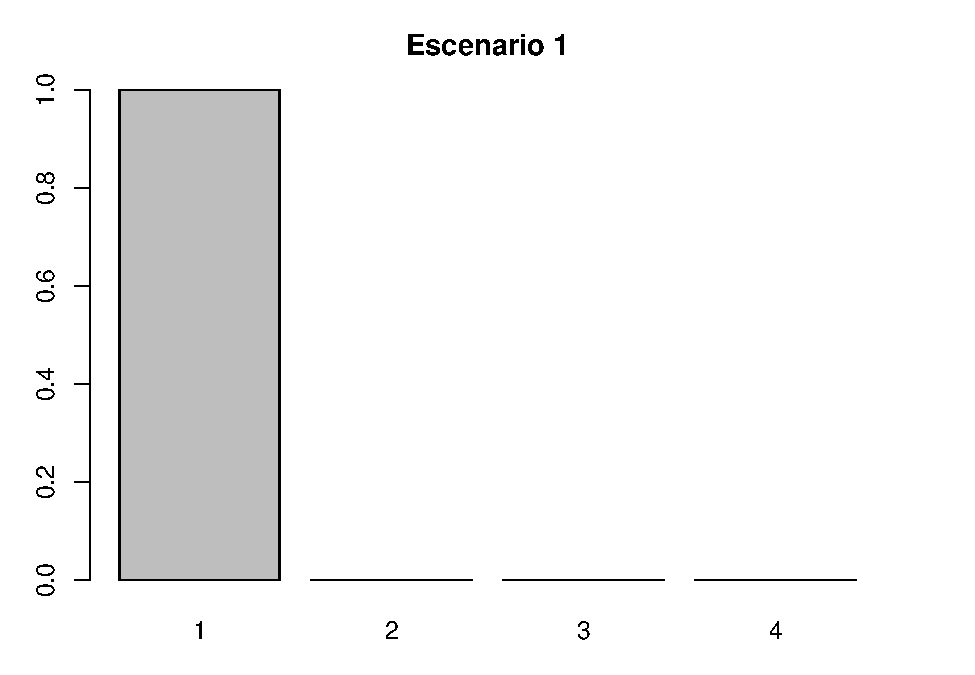
\includegraphics{Diagnostico_Poblacional_files/figure-latex/chap10_4-1.pdf}

\begin{Shaded}
\begin{Highlighting}[]
\CommentTok{\#Proyección de la dinámica escenario 1}
\NormalTok{pr1 }\OtherTok{\textless{}{-}} \FunctionTok{project}\NormalTok{(Lr1, }\AttributeTok{vector =}\NormalTok{ nLr1, }\AttributeTok{time =} \DecValTok{50}\NormalTok{)}
\FunctionTok{plot}\NormalTok{(pr1, }\AttributeTok{log =} \StringTok{"y"}\NormalTok{, }\AttributeTok{ylim =} \FunctionTok{c}\NormalTok{(}\FloatTok{0.1}\NormalTok{, }\FloatTok{1.6}\NormalTok{), }\AttributeTok{ann =} \ConstantTok{FALSE}\NormalTok{)}
\FunctionTok{title}\NormalTok{(}\AttributeTok{main =} \StringTok{"Proyección de la dinámica (Escenario 1)"}\NormalTok{, }\AttributeTok{xlab =} \StringTok{"Time intervals"}\NormalTok{, }\AttributeTok{ylab =} \StringTok{"Population size/density"}\NormalTok{)}
\end{Highlighting}
\end{Shaded}

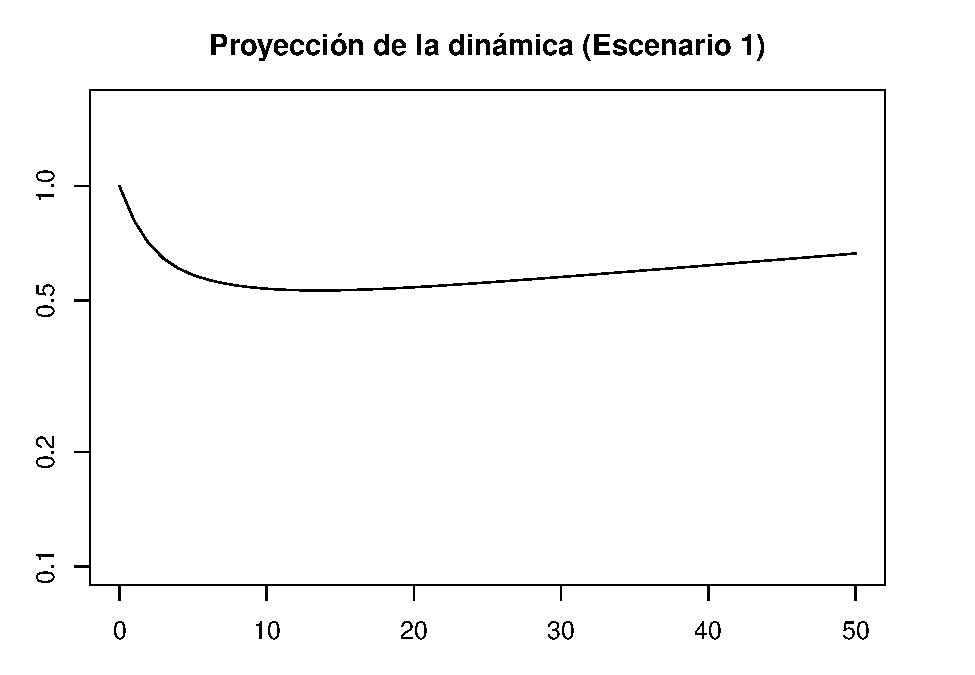
\includegraphics{Diagnostico_Poblacional_files/figure-latex/chap10_4-2.pdf}

\begin{Shaded}
\begin{Highlighting}[]
\CommentTok{\#Escenario 2. Inicio I}
\NormalTok{nLr2 }\OtherTok{\textless{}{-}} \FunctionTok{c}\NormalTok{(}\DecValTok{25}\NormalTok{, }\DecValTok{58}\NormalTok{, }\DecValTok{50}\NormalTok{, }\DecValTok{33}\NormalTok{)}
\CommentTok{\#Proporción de individuos por categoría}
\NormalTok{nLr2 }\OtherTok{\textless{}{-}}\NormalTok{ nLr2}\SpecialCharTok{/}\FunctionTok{sum}\NormalTok{(nLr2)}
\NormalTok{nLr2}
\end{Highlighting}
\end{Shaded}

\begin{verbatim}
## [1] 0.1506024 0.3493976 0.3012048 0.1987952
\end{verbatim}

\begin{Shaded}
\begin{Highlighting}[]
\CommentTok{\#Gráfica de barras del escenario 1 }
\FunctionTok{barplot}\NormalTok{(nLr2, }\AttributeTok{names.arg =} \DecValTok{1}\SpecialCharTok{:}\DecValTok{4}\NormalTok{)}
\FunctionTok{title}\NormalTok{( }\AttributeTok{main =} \StringTok{"Escenario 2"}\NormalTok{, }\AttributeTok{xlab =} \StringTok{"Categoría"}\NormalTok{, }\AttributeTok{ylab =} \StringTok{"Proporción"}\NormalTok{)}
\end{Highlighting}
\end{Shaded}

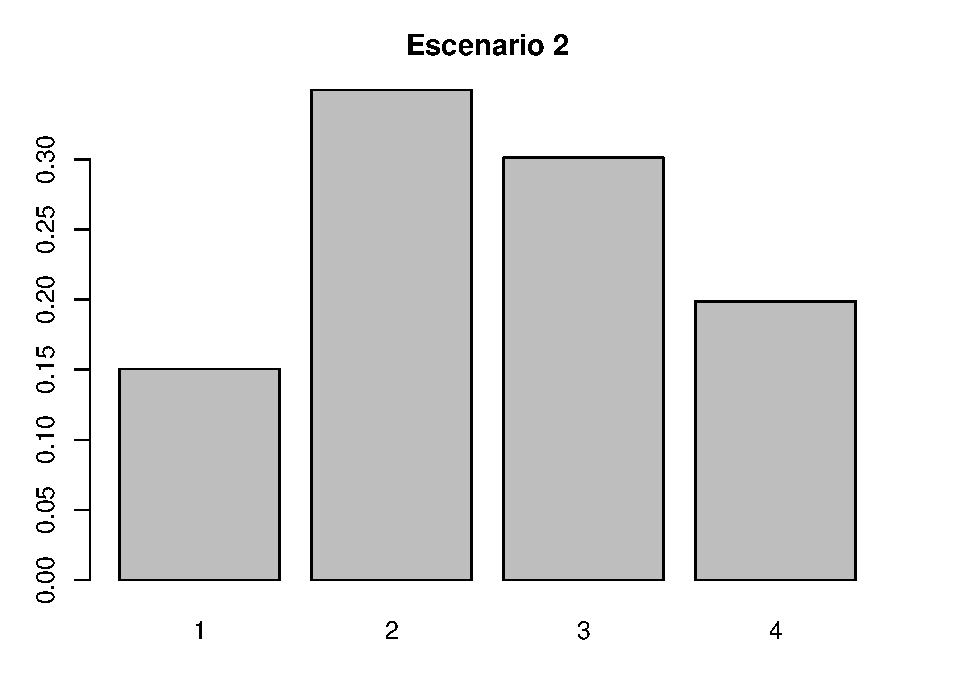
\includegraphics{Diagnostico_Poblacional_files/figure-latex/chap10_4-3.pdf}

\begin{Shaded}
\begin{Highlighting}[]
\CommentTok{\#Proyección de la dinámica escenario 2 }
\NormalTok{pr2 }\OtherTok{\textless{}{-}} \FunctionTok{project}\NormalTok{(Lr1, }\AttributeTok{vector =}\NormalTok{ nLr2, }\AttributeTok{time =} \DecValTok{50}\NormalTok{)}
\FunctionTok{plot}\NormalTok{(pr2, }\AttributeTok{log =} \StringTok{"y"}\NormalTok{, }\AttributeTok{ylim =} \FunctionTok{c}\NormalTok{(}\FloatTok{0.1}\NormalTok{, }\FloatTok{1.6}\NormalTok{), }\AttributeTok{ann =} \ConstantTok{FALSE}\NormalTok{)}
\FunctionTok{title}\NormalTok{(}\AttributeTok{main =} \StringTok{"Proyección de la dinámica (Escenario 2)"}\NormalTok{, }\AttributeTok{xlab =} \StringTok{"Time intervals"}\NormalTok{, }\AttributeTok{ylab =} \StringTok{"Population size/density"}\NormalTok{)}
\end{Highlighting}
\end{Shaded}

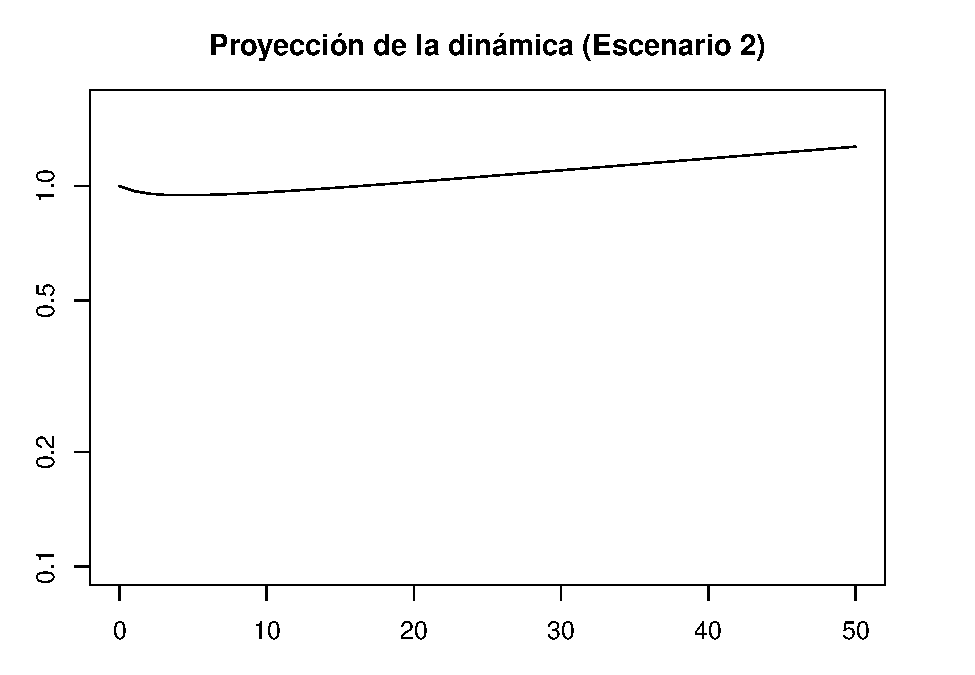
\includegraphics{Diagnostico_Poblacional_files/figure-latex/chap10_4-4.pdf}

\begin{Shaded}
\begin{Highlighting}[]
\CommentTok{\#Escenario 3. Estructura estable}
\CommentTok{\# Estructura estable de estados}
\NormalTok{Wmax }\OtherTok{\textless{}{-}} \FunctionTok{stable.stage}\NormalTok{(Lr1)}
\NormalTok{nLr3 }\OtherTok{\textless{}{-}}\NormalTok{ Wmax}
\CommentTok{\#Gráfica de barras del escenario 3}
\FunctionTok{barplot}\NormalTok{(nLr3, }\AttributeTok{names.arg =} \DecValTok{1}\SpecialCharTok{:}\DecValTok{4}\NormalTok{)}
\FunctionTok{title}\NormalTok{( }\AttributeTok{main =} \StringTok{"Escenario 3"}\NormalTok{, }\AttributeTok{xlab =} \StringTok{"Categoría"}\NormalTok{, }\AttributeTok{ylab =} \StringTok{"Proporción"}\NormalTok{)}
\end{Highlighting}
\end{Shaded}

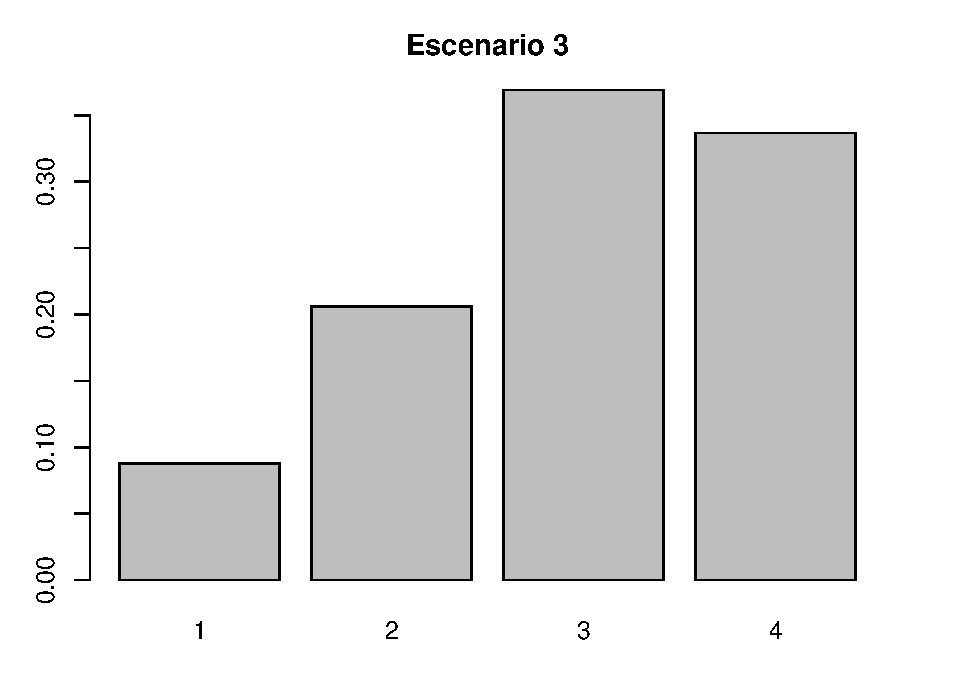
\includegraphics{Diagnostico_Poblacional_files/figure-latex/chap10_4-5.pdf}

\begin{Shaded}
\begin{Highlighting}[]
\CommentTok{\#Proyección de la dinámica escenario 3 }
\NormalTok{Lr1st }\OtherTok{\textless{}{-}}\NormalTok{ (Lr1}\SpecialCharTok{/}\NormalTok{lambda)}
\NormalTok{Lr1st}
\end{Highlighting}
\end{Shaded}

\begin{verbatim}
##           PL           J        NR        AR
## PL 0.4293064 0.000000000 0.0000000 0.1489268
## J  0.3756927 0.839848010 0.0000000 0.0000000
## NR 0.0000000 0.003375675 0.7897093 0.2283545
## AR 0.0000000 0.088363250 0.1827829 0.7456270
\end{verbatim}

\begin{Shaded}
\begin{Highlighting}[]
\FunctionTok{eigen}\NormalTok{(Lr1st)}
\end{Highlighting}
\end{Shaded}

\begin{verbatim}
## eigen() decomposition
## $values
## [1] 1.0000000+0.00000000i 0.8259670+0.00000000i 0.4892619+0.06421907i
## [4] 0.4892619-0.06421907i
## 
## $vectors
##               [,1]           [,2]                  [,3]                  [,4]
## [1,] -0.1605030+0i -0.03255031+0i -0.6050037+0.1108223i -0.6050037-0.1108223i
## [2,] -0.3765163+0i  0.88098064+0i  0.6483299+0.0000000i  0.6483299+0.0000000i
## [3,] -0.6739307+0i -0.46400142+0i  0.1712014+0.2009688i  0.1712014-0.2009688i
## [4,] -0.6150542+0i -0.08669643+0i -0.2913524-0.2162698i -0.2913524+0.2162698i
\end{verbatim}

\begin{Shaded}
\begin{Highlighting}[]
\NormalTok{pr3 }\OtherTok{\textless{}{-}} \FunctionTok{project}\NormalTok{(Lr1st, }\AttributeTok{vector =}\NormalTok{ Wmax, }\AttributeTok{time =} \DecValTok{50}\NormalTok{)}
\FunctionTok{plot}\NormalTok{(pr3, }\AttributeTok{log =} \StringTok{"y"}\NormalTok{, }\AttributeTok{ylim =} \FunctionTok{c}\NormalTok{(}\FloatTok{0.1}\NormalTok{, }\FloatTok{1.6}\NormalTok{), }\AttributeTok{ann =} \ConstantTok{FALSE}\NormalTok{)}
\FunctionTok{title}\NormalTok{(}\AttributeTok{main =} \StringTok{"Proyección de la dinámica (Escenario 3)"}\NormalTok{, }\AttributeTok{xlab =} \StringTok{"Time intervals"}\NormalTok{, }\AttributeTok{ylab =} \StringTok{"Population size/density"}\NormalTok{)}
\end{Highlighting}
\end{Shaded}

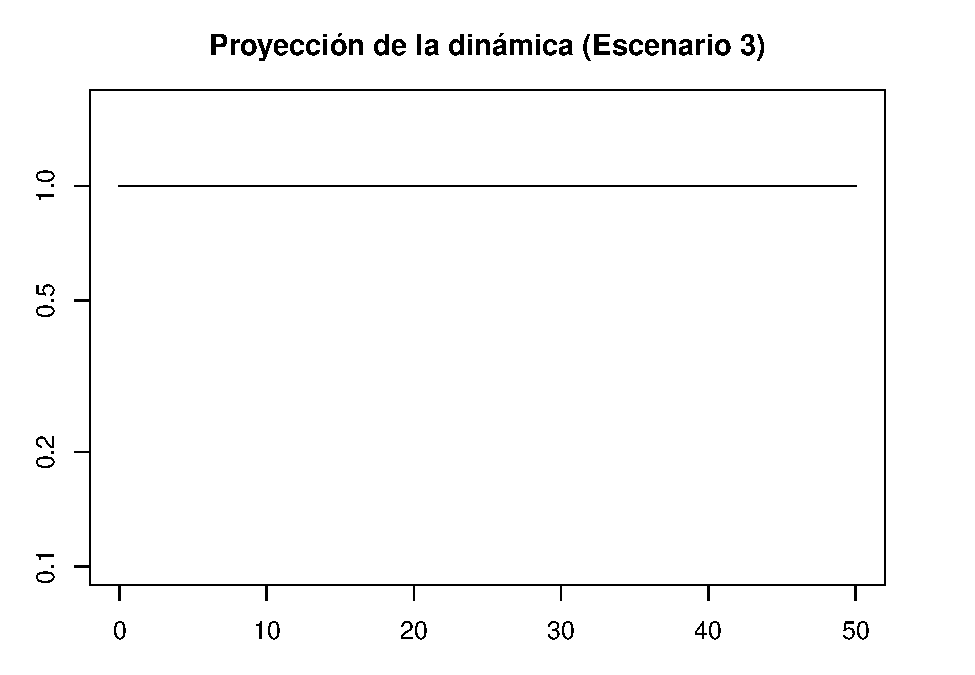
\includegraphics{Diagnostico_Poblacional_files/figure-latex/chap10_4-6.pdf}

\begin{Shaded}
\begin{Highlighting}[]
\CommentTok{\#Escenario 4. Inicio II}
\NormalTok{nLr4 }\OtherTok{\textless{}{-}} \FunctionTok{c}\NormalTok{(}\DecValTok{66}\NormalTok{, }\DecValTok{33}\NormalTok{, }\DecValTok{33}\NormalTok{, }\DecValTok{33}\NormalTok{)}
\CommentTok{\#Proporción de individuos por categoría}
\NormalTok{nLr4 }\OtherTok{\textless{}{-}}\NormalTok{ nLr4}\SpecialCharTok{/}\FunctionTok{sum}\NormalTok{(nLr4)}
\NormalTok{nLr4}
\end{Highlighting}
\end{Shaded}

\begin{verbatim}
## [1] 0.4 0.2 0.2 0.2
\end{verbatim}

\begin{Shaded}
\begin{Highlighting}[]
\CommentTok{\#Gráfica de barras del escenario 4 }
\FunctionTok{barplot}\NormalTok{(nLr4, }\AttributeTok{names.arg =} \DecValTok{1}\SpecialCharTok{:}\DecValTok{4}\NormalTok{)}
\FunctionTok{title}\NormalTok{( }\AttributeTok{main =} \StringTok{"Escenario 4"}\NormalTok{, }\AttributeTok{xlab =} \StringTok{"Categoría"}\NormalTok{, }\AttributeTok{ylab =} \StringTok{"Proporción"}\NormalTok{)}
\end{Highlighting}
\end{Shaded}

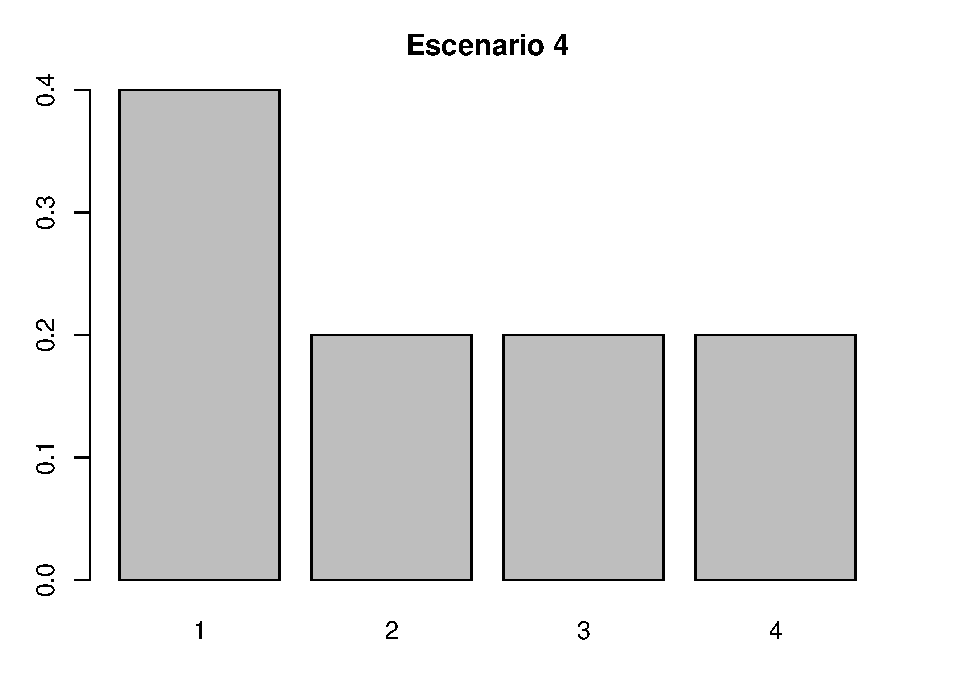
\includegraphics{Diagnostico_Poblacional_files/figure-latex/chap10_4-7.pdf}

\begin{Shaded}
\begin{Highlighting}[]
\CommentTok{\#Proyección de la dinámica escenario 4 }
\NormalTok{pr4 }\OtherTok{\textless{}{-}} \FunctionTok{project}\NormalTok{(Lr1, }\AttributeTok{vector =}\NormalTok{ nLr4, }\AttributeTok{time =} \DecValTok{50}\NormalTok{)}
\FunctionTok{plot}\NormalTok{(pr4, }\AttributeTok{log =} \StringTok{"y"}\NormalTok{, }\AttributeTok{ylim =} \FunctionTok{c}\NormalTok{(}\FloatTok{0.1}\NormalTok{, }\FloatTok{1.6}\NormalTok{), }\AttributeTok{ann =} \ConstantTok{FALSE}\NormalTok{)}
\FunctionTok{title}\NormalTok{(}\AttributeTok{main =} \StringTok{"Proyección de la dinámica (Escenario 4)"}\NormalTok{, }\AttributeTok{xlab =} \StringTok{"Time intervals"}\NormalTok{, }\AttributeTok{ylab =} \StringTok{"Population size/density"}\NormalTok{)}
\end{Highlighting}
\end{Shaded}

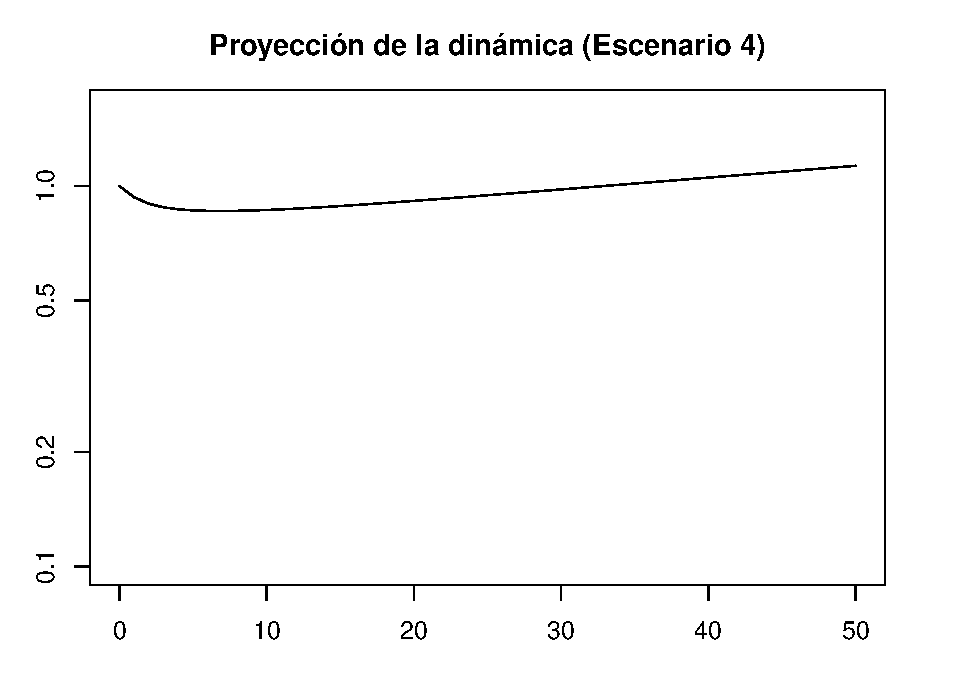
\includegraphics{Diagnostico_Poblacional_files/figure-latex/chap10_4-8.pdf}

\begin{Shaded}
\begin{Highlighting}[]
\CommentTok{\#Escenario 5. Límite superior}
\NormalTok{nLr5 }\OtherTok{\textless{}{-}} \FunctionTok{c}\NormalTok{(}\DecValTok{0}\NormalTok{, }\DecValTok{0}\NormalTok{, }\DecValTok{0}\NormalTok{, }\DecValTok{166}\NormalTok{)}
\CommentTok{\#Proporción de individuos por categoría}
\NormalTok{nLr5 }\OtherTok{\textless{}{-}}\NormalTok{ nLr5}\SpecialCharTok{/}\FunctionTok{sum}\NormalTok{(nLr5)}
\NormalTok{nLr5}
\end{Highlighting}
\end{Shaded}

\begin{verbatim}
## [1] 0 0 0 1
\end{verbatim}

\begin{Shaded}
\begin{Highlighting}[]
\CommentTok{\#Gráfica de barras del escenario 5 }
\FunctionTok{barplot}\NormalTok{(nLr5, }\AttributeTok{names.arg =} \DecValTok{1}\SpecialCharTok{:}\DecValTok{4}\NormalTok{)}
\FunctionTok{title}\NormalTok{( }\AttributeTok{main =} \StringTok{"Escenario 5"}\NormalTok{, }\AttributeTok{xlab =} \StringTok{"Categoría"}\NormalTok{, }\AttributeTok{ylab =} \StringTok{"Proporción"}\NormalTok{)}
\end{Highlighting}
\end{Shaded}

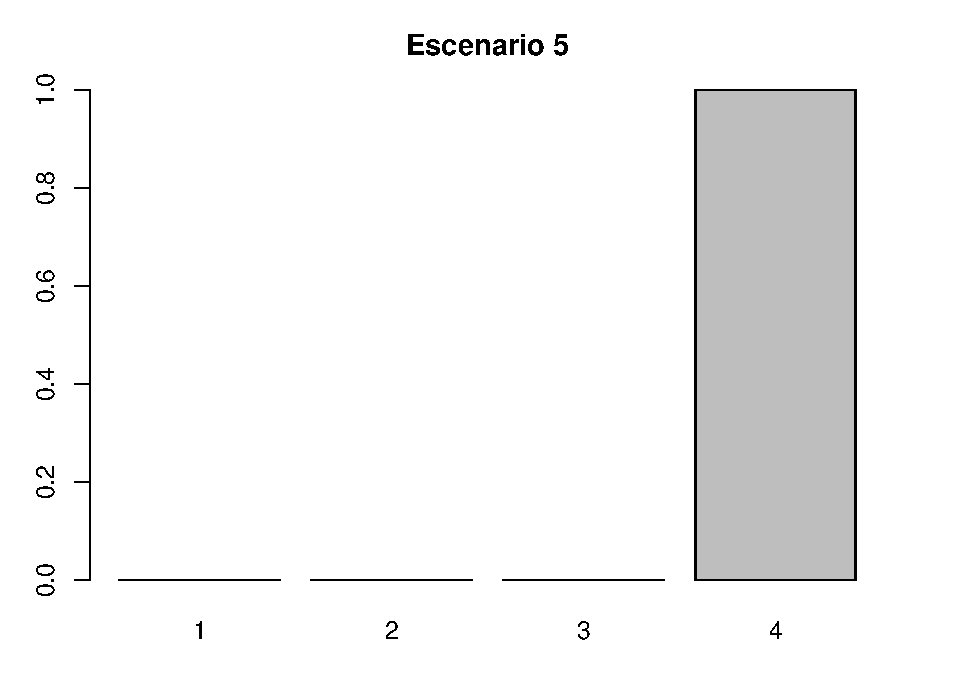
\includegraphics{Diagnostico_Poblacional_files/figure-latex/chap10_4-9.pdf}

\begin{Shaded}
\begin{Highlighting}[]
\CommentTok{\#Proyección de la dinámica escenario 5 }
\NormalTok{pr5 }\OtherTok{\textless{}{-}} \FunctionTok{project}\NormalTok{(Lr1, }\AttributeTok{vector =}\NormalTok{ nLr5, }\AttributeTok{time =} \DecValTok{50}\NormalTok{)}
\FunctionTok{plot}\NormalTok{(pr5, }\AttributeTok{log =} \StringTok{"y"}\NormalTok{, }\AttributeTok{ylim =} \FunctionTok{c}\NormalTok{(}\FloatTok{0.1}\NormalTok{, }\FloatTok{1.6}\NormalTok{), }\AttributeTok{ann =} \ConstantTok{FALSE}\NormalTok{)}
\FunctionTok{title}\NormalTok{(}\AttributeTok{main =} \StringTok{"Proyección de la dinámica (Escenario 5)"}\NormalTok{, }\AttributeTok{xlab =} \StringTok{"Time intervals"}\NormalTok{, }\AttributeTok{ylab =} \StringTok{"Population size/density"}\NormalTok{)}
\end{Highlighting}
\end{Shaded}

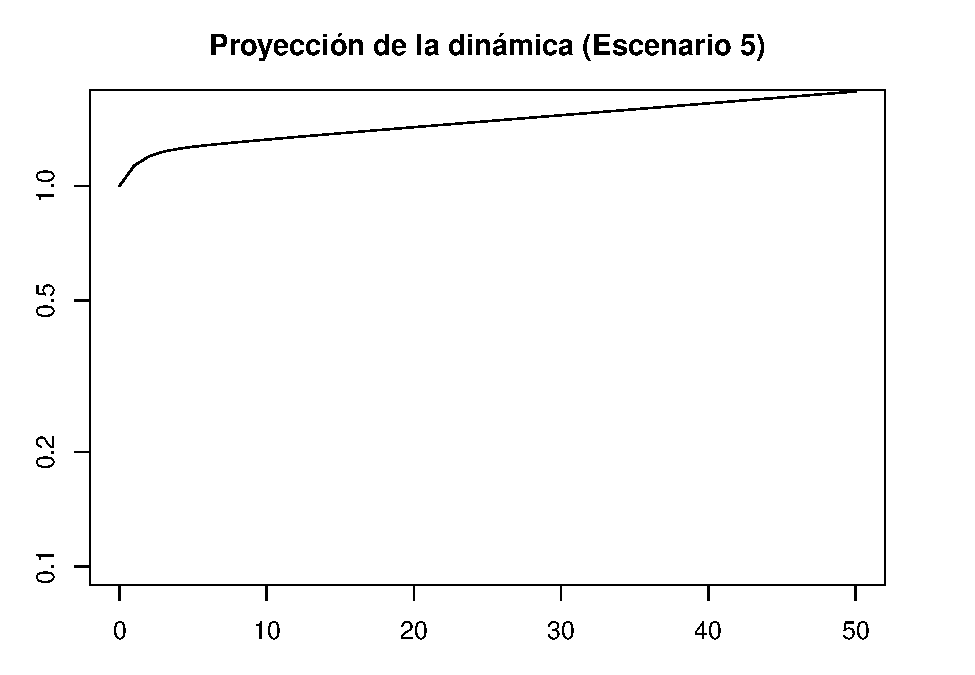
\includegraphics{Diagnostico_Poblacional_files/figure-latex/chap10_4-10.pdf}

\begin{Shaded}
\begin{Highlighting}[]
\CommentTok{\#Gráfica de la dinámica absoluta }
\NormalTok{Population\_density }\OtherTok{\textless{}{-}} \FunctionTok{stack}\NormalTok{(}\FunctionTok{c}\NormalTok{(}\FunctionTok{as.data.frame}\NormalTok{(pr1), }\FunctionTok{as.data.frame}\NormalTok{(pr2), }\FunctionTok{as.data.frame}\NormalTok{(pr3), }\FunctionTok{as.data.frame}\NormalTok{(pr4), }\FunctionTok{as.data.frame}\NormalTok{(pr5)))}
\NormalTok{Population\_density[, }\StringTok{"time"}\NormalTok{] }\OtherTok{\textless{}{-}} \FunctionTok{rep}\NormalTok{(}\FunctionTok{seq}\NormalTok{(}\DecValTok{1}\NormalTok{, }\FunctionTok{nrow}\NormalTok{(pr1), }\DecValTok{1}\NormalTok{), }\DecValTok{5}\NormalTok{)}
\FunctionTok{names}\NormalTok{(Population\_density) }\OtherTok{\textless{}{-}} \FunctionTok{c}\NormalTok{(}\StringTok{"Values"}\NormalTok{, }\StringTok{"Projection"}\NormalTok{, }\StringTok{"Time"}\NormalTok{)}
\CommentTok{\#Population\_density[, "Projection"] \textless{}{-} c(rep("Projection 1", len), rep("Projection 2", len), rep("Projection 3", len), rep("Projection 4", len), rep("Projection 5", len))}
\NormalTok{abs.plot }\OtherTok{\textless{}{-}} \FunctionTok{ggplot}\NormalTok{(}\AttributeTok{data =}\NormalTok{ Population\_density) }\SpecialCharTok{+}
\FunctionTok{theme\_classic}\NormalTok{() }\SpecialCharTok{+}
\FunctionTok{theme}\NormalTok{(}\AttributeTok{panel.border =} \FunctionTok{element\_blank}\NormalTok{()) }\SpecialCharTok{+}
\FunctionTok{theme}\NormalTok{(}\AttributeTok{legend.position =} \StringTok{"none"}\NormalTok{) }\SpecialCharTok{+}
\FunctionTok{geom\_line}\NormalTok{(}\FunctionTok{aes}\NormalTok{(}\AttributeTok{x =}\NormalTok{ Time, }\AttributeTok{y =}\NormalTok{ Values, }\AttributeTok{group =}\NormalTok{ Projection, }\AttributeTok{colour =}\NormalTok{ Projection), }\AttributeTok{linewidth =} \FloatTok{0.8}\NormalTok{) }\SpecialCharTok{+}
\FunctionTok{geom\_hline}\NormalTok{(}\AttributeTok{yintercept =} \DecValTok{1}\NormalTok{, }\AttributeTok{linewidth =} \FloatTok{0.8}\NormalTok{) }\SpecialCharTok{+}
\FunctionTok{scale\_colour\_manual}\NormalTok{(}\AttributeTok{values =} \FunctionTok{c}\NormalTok{(}\StringTok{"\#C6E2FF"}\NormalTok{, }\StringTok{"\#B9D3EE"}\NormalTok{, }\StringTok{"black"}\NormalTok{, }\StringTok{"\#9FB6CD"}\NormalTok{, }\StringTok{"\#6C7B8B"}\NormalTok{)) }\SpecialCharTok{+}
\FunctionTok{theme}\NormalTok{(}\AttributeTok{axis.title.x =} \FunctionTok{element\_text}\NormalTok{(}\AttributeTok{vjust =} \SpecialCharTok{{-}}\DecValTok{1}\NormalTok{, }\AttributeTok{size =} \DecValTok{12}\NormalTok{)) }\SpecialCharTok{+}
\FunctionTok{theme}\NormalTok{(}\AttributeTok{axis.title.y =} \FunctionTok{element\_text}\NormalTok{(}\AttributeTok{vjust =} \DecValTok{1}\NormalTok{, }\AttributeTok{size =} \DecValTok{12}\NormalTok{)) }\SpecialCharTok{+} 
\FunctionTok{theme}\NormalTok{(}\AttributeTok{axis.text =} \FunctionTok{element\_text}\NormalTok{(}\AttributeTok{size =} \DecValTok{12}\NormalTok{)) }\SpecialCharTok{+}
\FunctionTok{labs}\NormalTok{(}\AttributeTok{title =} \StringTok{"Absolut population dynamics"}\NormalTok{, }\AttributeTok{x =} \StringTok{"Projection intervals"}\NormalTok{, }\AttributeTok{y =} \StringTok{"Population density relative to lambda max"}\NormalTok{)}\SpecialCharTok{+} 
\FunctionTok{theme}\NormalTok{(}\AttributeTok{plot.title =} \FunctionTok{element\_text}\NormalTok{(}\AttributeTok{hjust =} \FloatTok{0.5}\NormalTok{, }\AttributeTok{face =} \StringTok{"bold"}\NormalTok{, }\AttributeTok{size =} \DecValTok{12}\NormalTok{))}
\NormalTok{abs.plot }
\end{Highlighting}
\end{Shaded}

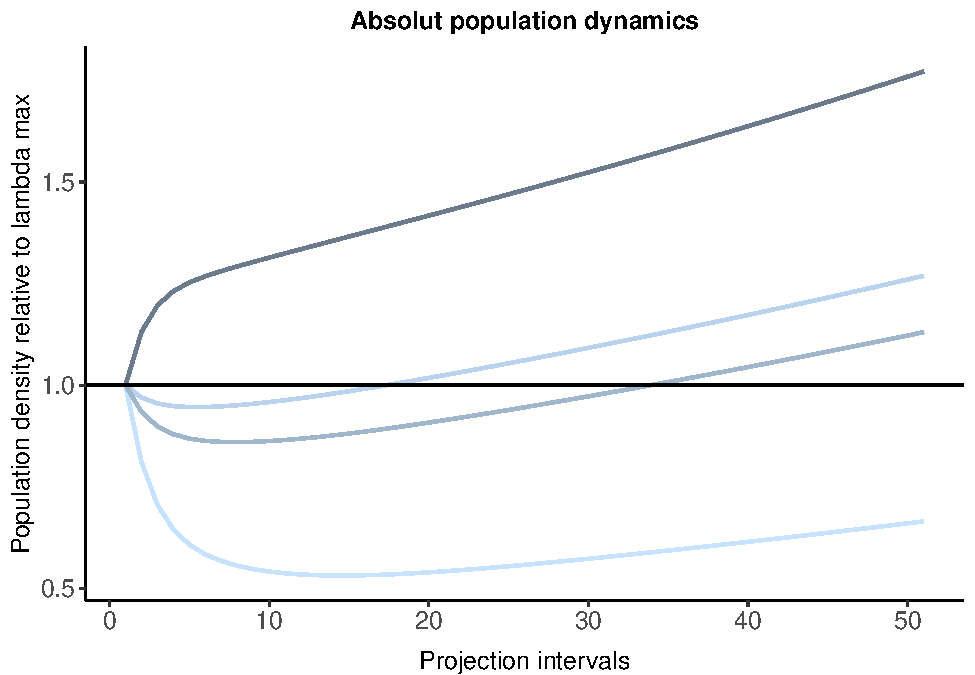
\includegraphics{Diagnostico_Poblacional_files/figure-latex/chap10_4-11.pdf}

\section{Dinámica transitoria estandarizada: límites}\label{dinuxe1mica-transitoria-estandarizada-luxedmites}

Con el fin de evaluar en el corto plazo los cambios cuantitativos en la población en respuesta a una perturbación determinada se calculan los límites de la dinámica transitoria a través Índices de transferencia y se proyecta el crecimiento de la población en el corto plazo.

\section{Dinámica transitoria específica de la población.}\label{dinuxe1mica-transitoria-especuxedfica-de-la-poblaciuxf3n.}

a proyección se hace sin la influencia de la dinámica asintótica. hecho que facilita y hace equitativa la comparación entre los modelos de los distintos escenarios. Se elimina el efecto de la dinámica asintótica al estandarizar la matriz y el vector de la estructura. En el primer caso se usa el comando `standard.A=T', lo cual supone que en el largo plazo la tasa de crecimiento poblacional tendrá un valor de 1 (unidad) -por lo que la población no crecerá ni declinará, en el segundo caso se usa el comando `standard.vec=T', que implica que éste suma 1 (Stoot et al., 2010, 2012). DINÁMICA POBLACIONAL TRANSITORIA ESTANDARIZADA

\emph{Índices de transferencia}. Con el fin de evaluar en el corto plazo qué cambios cuantitativos habría en la población como respuesta ante una perturbación determinada, se calculan los límites de la dinámica transitoria a través de los \emph{Índices de transferencia}, que incluyen los siguiente tres parámetros (Stoot et al.~2012):

\begin{enumerate}
\def\labelenumi{\alph{enumi})}
\item
  \emph{Reactividad alta y Reactividad baja} (Upper reactivity y Lower reactivity) que representan el crecimiento o el decremento inmediato (i.e.~primer intervalo de tiempo) de la población antes de alcanzar la tasa constante de crecimiento poblacional.
\item
  \emph{Máxima amplificación/Máxima atenuación} (Maximum amplification/Maximum attenuation) que indican,respectivamente, el incremento o decremento máximo futuro del crecimiento poblacional previo a alcanzar la tasa constante de crecimiento poblacional.
\item
  \emph{Inercia alta e Inercia baja} (Upper inertia y Lower inertia) que evalúan el límite más alto o el más bajo en el crecimiento de la población antes de alcanzar la tasa constante de crecimiento poblacional, respectivamente.
\end{enumerate}

\begin{Shaded}
\begin{Highlighting}[]
\DocumentationTok{\#\#\# PARTE II: DINÁMICA POBLACIONAL TRANSITORIA ESTANDARIZADA.}
\CommentTok{\#Modelo de Dinámica transitoria específica de la población  }
\DocumentationTok{\#\# La dinámica de corto plazo se projecta a partir de la matriz de transición y el vector inicial previamente definidos}

\CommentTok{\#Definir los margenes}
\FunctionTok{library}\NormalTok{(popdemo)}
\FunctionTok{library}\NormalTok{(ggplot2)}

\CommentTok{\#Vector de estructura inicial: abundancia por categoría de acuerdo con  el estado }
\NormalTok{n0 }\OtherTok{\textless{}{-}} \FunctionTok{c}\NormalTok{(}\DecValTok{0}\NormalTok{, }\DecValTok{46}\NormalTok{, }\DecValTok{38}\NormalTok{, }\DecValTok{82}\NormalTok{) }

\DocumentationTok{\#\# 1) PROYECCIÓN DE LA DINÁMICA DE CORTO PLAZO. Con la función PROJECT se proyectar la  a 50 meses, tomando en }
\CommentTok{\#cuenta la matriz de transición poblacional y el vector de la estructura.}
\CommentTok{\#En esta función se elimina el efecto de la dinámica asintótica al estandarizar: }
\CommentTok{\#a) la matriz usando el comando \textquotesingle{}standard.A=T\textquotesingle{}, lo cual significa que }
\CommentTok{\#en el largo plazo la tasa de crecimiento poblacional tendrá }
\CommentTok{\#un valor de 1 (unidad), por lo que la población no crecerá ni declinará. }
\CommentTok{\#b) el vector de la estructura usando \textquotesingle{}standard.vec=T\textquotesingle{}, lo cual supone que éste suma 1, }
\CommentTok{\# Ambas estandarizaciones facilitan y hacen equitativa la comparación entre modelos }
\CommentTok{\#con distintos tamaños poblacionales y distintas tasas de crecimiento de largo plazo. }

\CommentTok{\#Gráfica de la dinámica de corto plazo por escenario. En la graficación se usa la misma matriz pero se cambia el vector de acuerdo con el escenario}
\CommentTok{\#Escenario 1: Límite inferior}
\NormalTok{pr2}\FloatTok{.1} \OtherTok{\textless{}{-}} \FunctionTok{project}\NormalTok{(Lr1, }\AttributeTok{vector =}\NormalTok{ nLr1, }\AttributeTok{time =} \DecValTok{50}\NormalTok{, }
                 \AttributeTok{standard.A =}\NormalTok{ T, }\AttributeTok{standard.vec =}\NormalTok{ T)}
\CommentTok{\#Plot the amplification projection and label it}
\CommentTok{\# Se atenua (decrece)}
\FunctionTok{plot}\NormalTok{(pr2}\FloatTok{.1}\NormalTok{, }\AttributeTok{log =} \StringTok{"y"}\NormalTok{, }\AttributeTok{main =} \StringTok{"Dinámica a corto plazo (Escenario 1)"}\NormalTok{, }\AttributeTok{cex.axis =} \FloatTok{0.8}\NormalTok{)}
\end{Highlighting}
\end{Shaded}

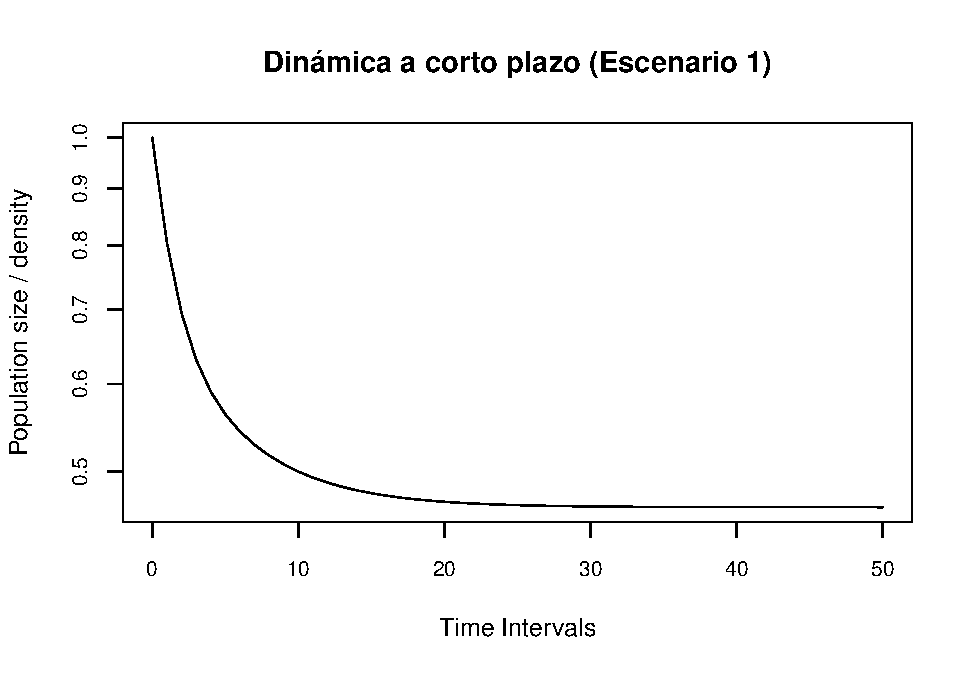
\includegraphics{Diagnostico_Poblacional_files/figure-latex/chap10_5-1.pdf}

\begin{Shaded}
\begin{Highlighting}[]
\CommentTok{\#Escenario 2. Inicio I}
\NormalTok{pr2}\FloatTok{.2} \OtherTok{\textless{}{-}} \FunctionTok{project}\NormalTok{(Lr1, }\AttributeTok{vector =}\NormalTok{ nLr2, }\AttributeTok{time =} \DecValTok{50}\NormalTok{, }
                 \AttributeTok{standard.A =}\NormalTok{ T, }\AttributeTok{standard.vec =}\NormalTok{ T)}
\CommentTok{\#Plot the amplification projection and label it}
\FunctionTok{plot}\NormalTok{(pr2}\FloatTok{.2}\NormalTok{, }\AttributeTok{log =} \StringTok{"y"}\NormalTok{, }\AttributeTok{main =} \StringTok{"Dinámica a corto plazo (Escenario 2)"}\NormalTok{, }\AttributeTok{cex.axis =} \FloatTok{0.8}\NormalTok{) }\CommentTok{\# Se atenua (decrece)}
\end{Highlighting}
\end{Shaded}

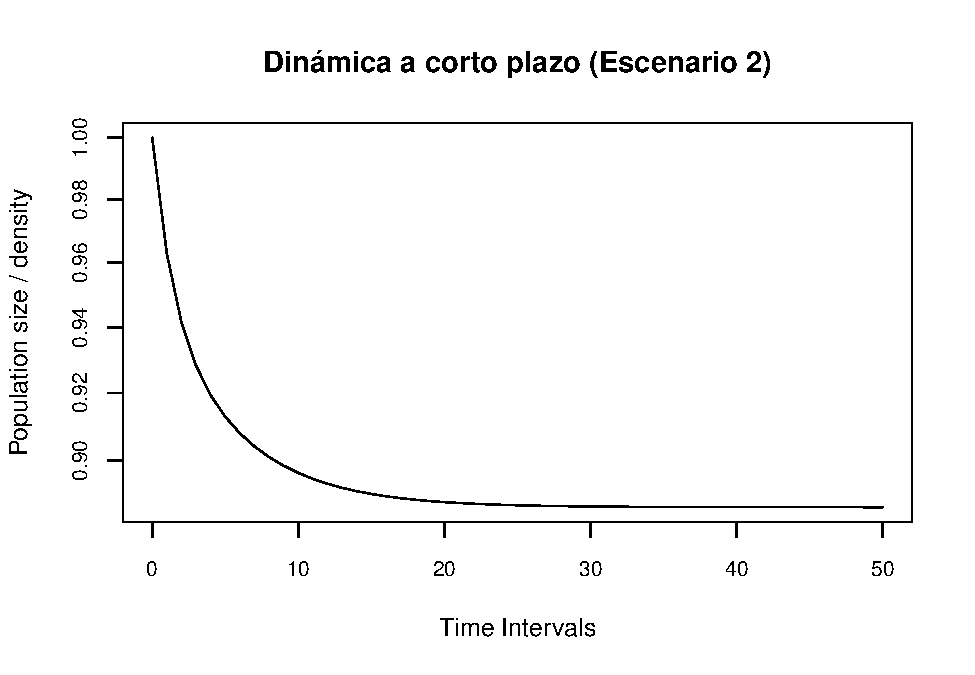
\includegraphics{Diagnostico_Poblacional_files/figure-latex/chap10_5-2.pdf}

\begin{Shaded}
\begin{Highlighting}[]
\CommentTok{\#Escenario 3. Estructura estable}
\NormalTok{pr2}\FloatTok{.3} \OtherTok{\textless{}{-}} \FunctionTok{project}\NormalTok{(Lr1, }\AttributeTok{vector =}\NormalTok{ nLr3, }\AttributeTok{time =} \DecValTok{50}\NormalTok{, }
                 \AttributeTok{standard.A =}\NormalTok{ T, }\AttributeTok{standard.vec =}\NormalTok{ T)}
\CommentTok{\#Plot the amplification projection and label it}
\FunctionTok{plot}\NormalTok{(pr2}\FloatTok{.3}\NormalTok{, }\AttributeTok{main =} \StringTok{"Dinámica a corto plazo (Escenario 3)"}\NormalTok{, }\AttributeTok{cex.axis =} \FloatTok{0.8}\NormalTok{)}\CommentTok{\# Se amplifica (crece)}
\end{Highlighting}
\end{Shaded}

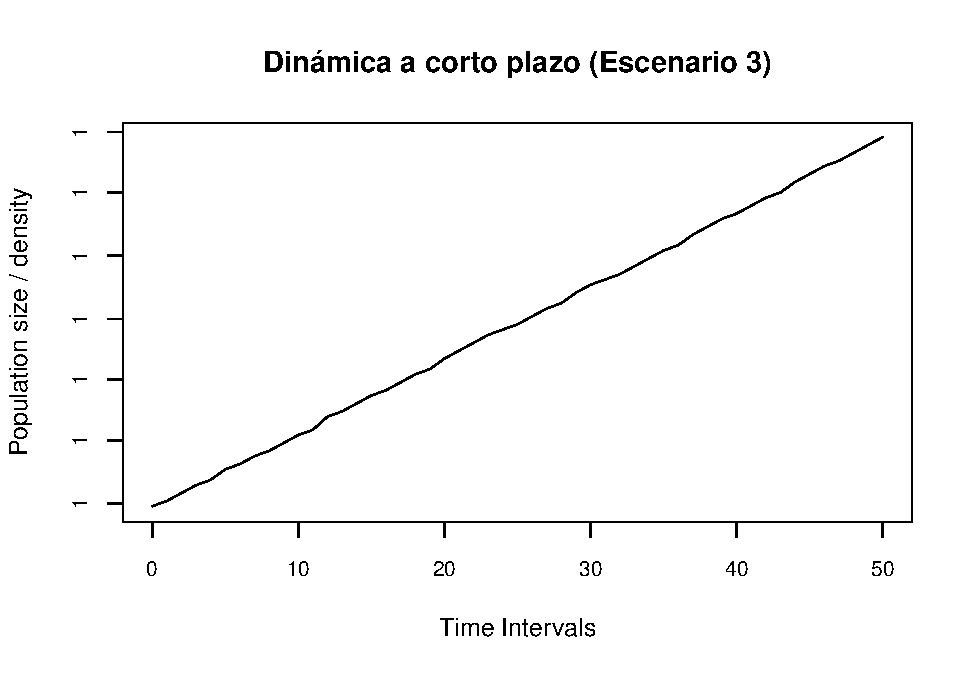
\includegraphics{Diagnostico_Poblacional_files/figure-latex/chap10_5-3.pdf}

\begin{Shaded}
\begin{Highlighting}[]
\CommentTok{\#Escenario 4. Inicio II}
\NormalTok{pr2}\FloatTok{.4} \OtherTok{\textless{}{-}} \FunctionTok{project}\NormalTok{(Lr1, }\AttributeTok{vector =}\NormalTok{ nLr4, }\AttributeTok{time =} \DecValTok{50}\NormalTok{, }
                 \AttributeTok{standard.A =}\NormalTok{ T, }\AttributeTok{standard.vec =}\NormalTok{ T)}
\CommentTok{\#Plot the amplification projection and label it}
\FunctionTok{plot}\NormalTok{(pr2}\FloatTok{.4}\NormalTok{, }\AttributeTok{log =} \StringTok{"y"}\NormalTok{, }\AttributeTok{main =} \StringTok{"Dinámica a corto plazo (Escenario 4)"}\NormalTok{, }\AttributeTok{cex.axis =} \FloatTok{0.8}\NormalTok{)}\CommentTok{\# Se atenua (decrece)}
\end{Highlighting}
\end{Shaded}

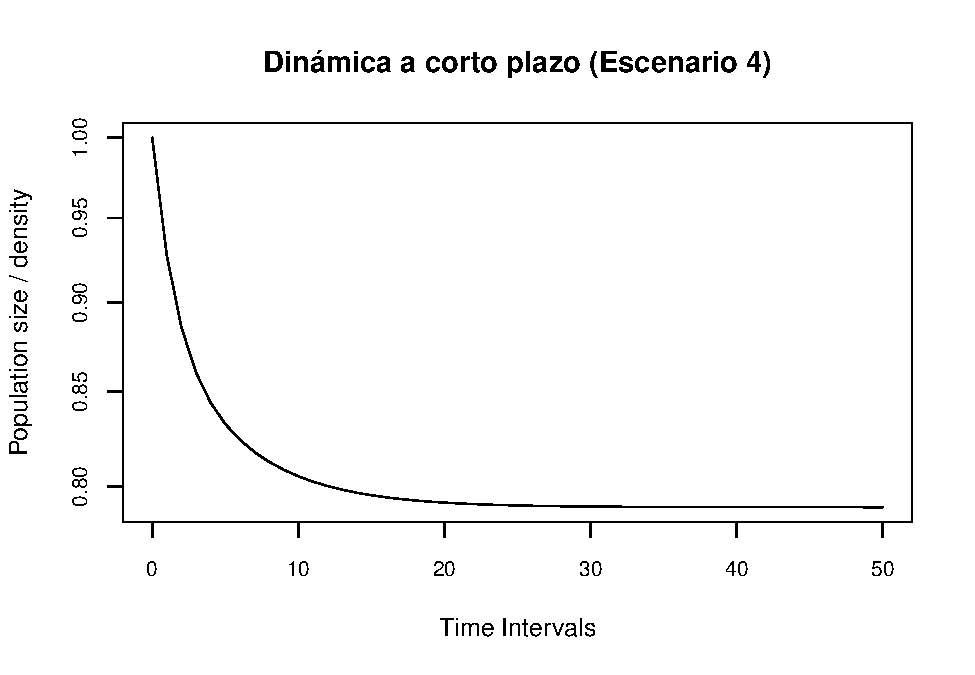
\includegraphics{Diagnostico_Poblacional_files/figure-latex/chap10_5-4.pdf}

\begin{Shaded}
\begin{Highlighting}[]
\CommentTok{\#Escenario 5. Límite superior}
\NormalTok{pr2}\FloatTok{.5} \OtherTok{\textless{}{-}} \FunctionTok{project}\NormalTok{(Lr1, }\AttributeTok{vector =}\NormalTok{ nLr5, }\AttributeTok{time =} \DecValTok{50}\NormalTok{, }
                 \AttributeTok{standard.A =}\NormalTok{ T, }\AttributeTok{standard.vec =}\NormalTok{ T)}
\CommentTok{\#Plot the amplification projection and label it}
\FunctionTok{plot}\NormalTok{(pr2}\FloatTok{.5}\NormalTok{, }\AttributeTok{log =} \StringTok{"y"}\NormalTok{, }\AttributeTok{main =} \StringTok{"Dinámica a corto plazo (Escenario 5)"}\NormalTok{, }\AttributeTok{cex.axis =} \FloatTok{0.8}\NormalTok{)}\CommentTok{\# Se amplifica (crece)}
\end{Highlighting}
\end{Shaded}

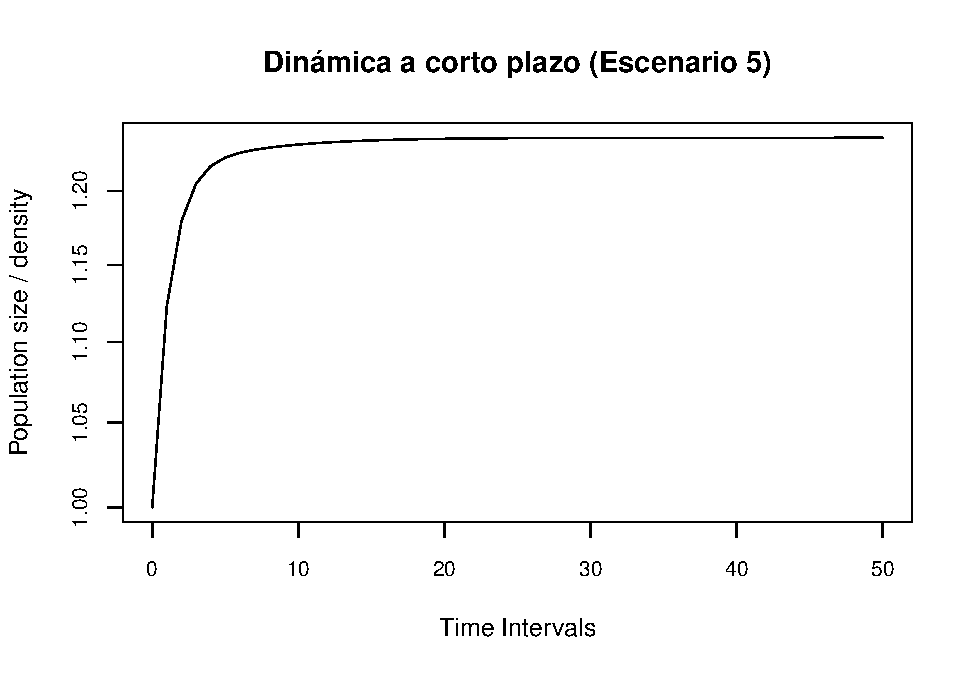
\includegraphics{Diagnostico_Poblacional_files/figure-latex/chap10_5-5.pdf}

\begin{Shaded}
\begin{Highlighting}[]
\CommentTok{\#2) LIMITES TRANSITORIOS POR ESCENARIO.}
\CommentTok{\#Escenario 1: Límite inferior}

\CommentTok{\#Cálculo de los limites transitorios}
\FunctionTok{library}\NormalTok{(popdemo)}

\NormalTok{lim.trans }\OtherTok{\textless{}{-}} \FunctionTok{as.data.frame}\NormalTok{(}\FunctionTok{matrix}\NormalTok{(}\ConstantTok{NA}\NormalTok{, }\DecValTok{5}\NormalTok{, }\DecValTok{3}\NormalTok{))}
\FunctionTok{names}\NormalTok{(lim.trans) }\OtherTok{\textless{}{-}} \FunctionTok{c}\NormalTok{(}\StringTok{"reac"}\NormalTok{, }\StringTok{"maxatt"}\NormalTok{, }\StringTok{"inertia"}\NormalTok{)}
\NormalTok{reac1}\OtherTok{\textless{}{-}}\FunctionTok{reac}\NormalTok{(Lr1, }\AttributeTok{vector =}\NormalTok{ nLr1)}
\NormalTok{lim.trans[}\DecValTok{1}\NormalTok{, }\DecValTok{1}\NormalTok{] }\OtherTok{\textless{}{-}}\NormalTok{ reac1}
\NormalTok{reac1}
\end{Highlighting}
\end{Shaded}

\begin{verbatim}
## [1] 0.8049991
\end{verbatim}

\begin{Shaded}
\begin{Highlighting}[]
\NormalTok{maxatt1}\OtherTok{\textless{}{-}}\FunctionTok{maxatt}\NormalTok{(Lr1, }\AttributeTok{vector =}\NormalTok{ nLr1, }\AttributeTok{return.t=}\NormalTok{T)}
\NormalTok{maxatt1}
\end{Highlighting}
\end{Shaded}

\begin{verbatim}
## $maxatt
## [1] 0.4643848
## 
## $t
## [1] 49
\end{verbatim}

\begin{Shaded}
\begin{Highlighting}[]
\NormalTok{lim.trans[}\DecValTok{1}\NormalTok{, }\DecValTok{2}\NormalTok{] }\OtherTok{\textless{}{-}}\NormalTok{ maxatt1[}\DecValTok{1}\NormalTok{]}
\NormalTok{inertia1}\OtherTok{\textless{}{-}}\FunctionTok{inertia}\NormalTok{(Lr1, }\AttributeTok{vector =}\NormalTok{ nLr1)}
\NormalTok{inertia1}
\end{Highlighting}
\end{Shaded}

\begin{verbatim}
## [1] 0.4643642
\end{verbatim}

\begin{Shaded}
\begin{Highlighting}[]
\NormalTok{lim.trans[}\DecValTok{1}\NormalTok{, }\DecValTok{3}\NormalTok{] }\OtherTok{\textless{}{-}}\NormalTok{ inertia1}
\CommentTok{\#Escenario 2. Inicio I}
\NormalTok{reac2}\OtherTok{\textless{}{-}}\FunctionTok{reac}\NormalTok{(Lr1, }\AttributeTok{vector =}\NormalTok{ nLr2)}
\NormalTok{reac2}
\end{Highlighting}
\end{Shaded}

\begin{verbatim}
## [1] 0.9628771
\end{verbatim}

\begin{Shaded}
\begin{Highlighting}[]
\NormalTok{lim.trans[}\DecValTok{2}\NormalTok{, }\DecValTok{1}\NormalTok{] }\OtherTok{\textless{}{-}}\NormalTok{ reac2}
\NormalTok{maxatt2}\OtherTok{\textless{}{-}}\FunctionTok{maxatt}\NormalTok{(Lr1, }\AttributeTok{vector =}\NormalTok{ nLr2, }\AttributeTok{return.t=}\NormalTok{T)}
\NormalTok{maxatt2}
\end{Highlighting}
\end{Shaded}

\begin{verbatim}
## $maxatt
## [1] 0.8863718
## 
## $t
## [1] 39
\end{verbatim}

\begin{Shaded}
\begin{Highlighting}[]
\NormalTok{lim.trans[}\DecValTok{2}\NormalTok{, }\DecValTok{2}\NormalTok{] }\OtherTok{\textless{}{-}}\NormalTok{ maxatt2[}\DecValTok{1}\NormalTok{]}
\NormalTok{inertia2}\OtherTok{\textless{}{-}}\FunctionTok{inertia}\NormalTok{(Lr1, }\AttributeTok{vector =}\NormalTok{ nLr2)}
\NormalTok{inertia2}
\end{Highlighting}
\end{Shaded}

\begin{verbatim}
## [1] 0.8863327
\end{verbatim}

\begin{Shaded}
\begin{Highlighting}[]
\NormalTok{lim.trans[}\DecValTok{2}\NormalTok{, }\DecValTok{3}\NormalTok{] }\OtherTok{\textless{}{-}}\NormalTok{ inertia2}

\CommentTok{\#Escenario 3. Estructura estable}
\NormalTok{reac3}\OtherTok{\textless{}{-}}\FunctionTok{reac}\NormalTok{(Lr1, }\AttributeTok{vector =}\NormalTok{ nLr3)}
\NormalTok{lim.trans[}\DecValTok{3}\NormalTok{, }\DecValTok{1}\NormalTok{] }\OtherTok{\textless{}{-}}\NormalTok{ reac1}
\NormalTok{reac3}
\end{Highlighting}
\end{Shaded}

\begin{verbatim}
## [1] 1
\end{verbatim}

\begin{Shaded}
\begin{Highlighting}[]
\NormalTok{maxamp3}\OtherTok{\textless{}{-}}\FunctionTok{maxamp}\NormalTok{(Lr1, }\AttributeTok{vector =}\NormalTok{ nLr3, }\AttributeTok{return.t=}\NormalTok{T)}
\NormalTok{maxamp3}
\end{Highlighting}
\end{Shaded}

\begin{verbatim}
## $maxamp
## [1] 1
## 
## $t
## [1] 1
\end{verbatim}

\begin{Shaded}
\begin{Highlighting}[]
\NormalTok{lim.trans[}\DecValTok{3}\NormalTok{, }\DecValTok{2}\NormalTok{] }\OtherTok{\textless{}{-}}\NormalTok{ maxamp3[}\DecValTok{1}\NormalTok{]}
\NormalTok{inertia3}\OtherTok{\textless{}{-}}\FunctionTok{inertia}\NormalTok{(Lr1, }\AttributeTok{vector =}\NormalTok{ nLr3)}
\NormalTok{inertia3}
\end{Highlighting}
\end{Shaded}

\begin{verbatim}
## [1] 1
\end{verbatim}

\begin{Shaded}
\begin{Highlighting}[]
\NormalTok{lim.trans[}\DecValTok{3}\NormalTok{, }\DecValTok{3}\NormalTok{] }\OtherTok{\textless{}{-}}\NormalTok{ inertia3}

\CommentTok{\#Escenario 4. Inicio II}
\NormalTok{reac4}\OtherTok{\textless{}{-}}\FunctionTok{reac}\NormalTok{(Lr1, }\AttributeTok{vector =}\NormalTok{ nLr4)}
\NormalTok{lim.trans[}\DecValTok{4}\NormalTok{, }\DecValTok{1}\NormalTok{] }\OtherTok{\textless{}{-}}\NormalTok{ reac1}
\NormalTok{reac4}
\end{Highlighting}
\end{Shaded}

\begin{verbatim}
## [1] 0.9273971
\end{verbatim}

\begin{Shaded}
\begin{Highlighting}[]
\NormalTok{maxatt4}\OtherTok{\textless{}{-}}\FunctionTok{maxatt}\NormalTok{(Lr1, }\AttributeTok{vector =}\NormalTok{ nLr4, }\AttributeTok{return.t=}\NormalTok{T)}
\NormalTok{maxatt4}
\end{Highlighting}
\end{Shaded}

\begin{verbatim}
## $maxatt
## [1] 0.7894384
## 
## $t
## [1] 42
\end{verbatim}

\begin{Shaded}
\begin{Highlighting}[]
\NormalTok{lim.trans[}\DecValTok{4}\NormalTok{, }\DecValTok{2}\NormalTok{] }\OtherTok{\textless{}{-}}\NormalTok{ maxatt4[}\DecValTok{1}\NormalTok{]}
\NormalTok{inertia4}\OtherTok{\textless{}{-}}\FunctionTok{inertia}\NormalTok{(Lr1, }\AttributeTok{vector =}\NormalTok{ nLr4)}
\NormalTok{inertia4}
\end{Highlighting}
\end{Shaded}

\begin{verbatim}
## [1] 0.7894036
\end{verbatim}

\begin{Shaded}
\begin{Highlighting}[]
\NormalTok{lim.trans[}\DecValTok{4}\NormalTok{, }\DecValTok{3}\NormalTok{] }\OtherTok{\textless{}{-}}\NormalTok{ inertia4}

\CommentTok{\#Escenario 5. Límite superior}
\NormalTok{reac5}\OtherTok{\textless{}{-}}\FunctionTok{reac}\NormalTok{(Lr1, }\AttributeTok{vector =}\NormalTok{ nLr5)}
\NormalTok{lim.trans[}\DecValTok{5}\NormalTok{, }\DecValTok{1}\NormalTok{] }\OtherTok{\textless{}{-}}\NormalTok{ reac5}
\NormalTok{reac5}
\end{Highlighting}
\end{Shaded}

\begin{verbatim}
## [1] 1.122908
\end{verbatim}

\begin{Shaded}
\begin{Highlighting}[]
\NormalTok{maxamp5}\OtherTok{\textless{}{-}}\FunctionTok{maxamp}\NormalTok{(Lr1, }\AttributeTok{vector =}\NormalTok{ nLr5, }\AttributeTok{return.t=}\NormalTok{T)}
\NormalTok{maxamp5}
\end{Highlighting}
\end{Shaded}

\begin{verbatim}
## $maxamp
## [1] 1.23733
## 
## $t
## [1] 34
\end{verbatim}

\begin{Shaded}
\begin{Highlighting}[]
\NormalTok{lim.trans[}\DecValTok{5}\NormalTok{, }\DecValTok{2}\NormalTok{] }\OtherTok{\textless{}{-}}\NormalTok{ maxamp5[}\DecValTok{1}\NormalTok{]}
\NormalTok{inertia5}\OtherTok{\textless{}{-}}\FunctionTok{inertia}\NormalTok{(Lr1, }\AttributeTok{vector =}\NormalTok{ nLr3)}
\NormalTok{inertia5}
\end{Highlighting}
\end{Shaded}

\begin{verbatim}
## [1] 1
\end{verbatim}

\begin{Shaded}
\begin{Highlighting}[]
\NormalTok{lim.trans[}\DecValTok{5}\NormalTok{, }\DecValTok{3}\NormalTok{] }\OtherTok{\textless{}{-}}\NormalTok{ inertia5}

\CommentTok{\# Dinamica transitoria plot}
\NormalTok{len }\OtherTok{\textless{}{-}} \FunctionTok{nrow}\NormalTok{(pr2}\FloatTok{.1}\NormalTok{)}
\NormalTok{Population\_density }\OtherTok{\textless{}{-}} \FunctionTok{stack}\NormalTok{(}\FunctionTok{c}\NormalTok{(}\FunctionTok{as.data.frame}\NormalTok{(pr2}\FloatTok{.1}\NormalTok{), }\FunctionTok{as.data.frame}\NormalTok{(pr2}\FloatTok{.2}\NormalTok{), }\FunctionTok{as.data.frame}\NormalTok{(pr2}\FloatTok{.3}\NormalTok{), }\FunctionTok{as.data.frame}\NormalTok{(pr2}\FloatTok{.4}\NormalTok{), }\FunctionTok{as.data.frame}\NormalTok{(pr2}\FloatTok{.5}\NormalTok{)))}
\NormalTok{Population\_density[, }\StringTok{"time"}\NormalTok{] }\OtherTok{\textless{}{-}} \FunctionTok{rep}\NormalTok{(}\FunctionTok{seq}\NormalTok{(}\DecValTok{1}\NormalTok{, len, }\DecValTok{1}\NormalTok{), }\DecValTok{5}\NormalTok{)}
\FunctionTok{names}\NormalTok{(Population\_density) }\OtherTok{\textless{}{-}} \FunctionTok{c}\NormalTok{(}\StringTok{"Values"}\NormalTok{, }\StringTok{"Projection"}\NormalTok{, }\StringTok{"Time"}\NormalTok{)}
\NormalTok{Population\_density[, }\StringTok{"Projection"}\NormalTok{] }\OtherTok{\textless{}{-}} \FunctionTok{c}\NormalTok{(}\FunctionTok{rep}\NormalTok{(}\StringTok{"Projection 1"}\NormalTok{, len), }\FunctionTok{rep}\NormalTok{(}\StringTok{"Projection 2"}\NormalTok{, len), }\FunctionTok{rep}\NormalTok{(}\StringTok{"Projection 3"}\NormalTok{, len), }\FunctionTok{rep}\NormalTok{(}\StringTok{"Projection 4"}\NormalTok{, len), }\FunctionTok{rep}\NormalTok{(}\StringTok{"Projection 5"}\NormalTok{, len))}

\NormalTok{trans.plot }\OtherTok{\textless{}{-}} \FunctionTok{ggplot}\NormalTok{(}\AttributeTok{data =}\NormalTok{ Population\_density) }\SpecialCharTok{+}
\FunctionTok{theme\_classic}\NormalTok{() }\SpecialCharTok{+}
\FunctionTok{theme}\NormalTok{(}\AttributeTok{panel.border =} \FunctionTok{element\_blank}\NormalTok{()) }\SpecialCharTok{+}
\FunctionTok{theme}\NormalTok{(}\AttributeTok{legend.position =} \StringTok{"none"}\NormalTok{) }\SpecialCharTok{+}
\FunctionTok{geom\_line}\NormalTok{(}\FunctionTok{aes}\NormalTok{(}\AttributeTok{x =}\NormalTok{ Time, }\AttributeTok{y =}\NormalTok{ Values, }\AttributeTok{group =}\NormalTok{ Projection, }\AttributeTok{colour =}\NormalTok{ Projection), }\AttributeTok{linewidth =} \FloatTok{0.8}\NormalTok{) }\SpecialCharTok{+}
\FunctionTok{scale\_colour\_manual}\NormalTok{(}\AttributeTok{values =} \FunctionTok{c}\NormalTok{(}\StringTok{"\#C6E2FF"}\NormalTok{, }\StringTok{"\#B9D3EE"}\NormalTok{, }\StringTok{"black"}\NormalTok{, }\StringTok{"\#9FB6CD"}\NormalTok{, }\StringTok{"\#6C7B8B"}\NormalTok{)) }\SpecialCharTok{+}
\FunctionTok{theme}\NormalTok{(}\AttributeTok{axis.title.x =} \FunctionTok{element\_text}\NormalTok{(}\AttributeTok{vjust =} \SpecialCharTok{{-}}\DecValTok{1}\NormalTok{, }\AttributeTok{size =} \DecValTok{12}\NormalTok{)) }\SpecialCharTok{+}
\FunctionTok{theme}\NormalTok{(}\AttributeTok{axis.title.y =} \FunctionTok{element\_text}\NormalTok{(}\AttributeTok{vjust =} \DecValTok{1}\NormalTok{, }\AttributeTok{size =} \DecValTok{12}\NormalTok{)) }\SpecialCharTok{+} 
\FunctionTok{theme}\NormalTok{(}\AttributeTok{axis.text =} \FunctionTok{element\_text}\NormalTok{(}\AttributeTok{size =} \DecValTok{15}\NormalTok{)) }\SpecialCharTok{+}
\FunctionTok{labs}\NormalTok{(}\AttributeTok{title =} \StringTok{"Transient population dynamics"}\NormalTok{ ,}\AttributeTok{x =} \StringTok{"Projection intervals"}\NormalTok{, }\AttributeTok{y =} \StringTok{"Population density relative to lambda max"}\NormalTok{) }\SpecialCharTok{+} 
\FunctionTok{theme}\NormalTok{(}\AttributeTok{plot.title =} \FunctionTok{element\_text}\NormalTok{(}\AttributeTok{hjust =} \FloatTok{0.5}\NormalTok{, }\AttributeTok{face =} \StringTok{"bold"}\NormalTok{, }\AttributeTok{size =} \DecValTok{12}\NormalTok{)) }\SpecialCharTok{+}
\FunctionTok{ylim}\NormalTok{(}\FloatTok{0.2}\NormalTok{, }\FloatTok{1.5}\NormalTok{)}
\NormalTok{trans.plot }\SpecialCharTok{+} 
\FunctionTok{geom\_text}\NormalTok{(}\AttributeTok{x =} \DecValTok{45}\NormalTok{, }\AttributeTok{y =} \FloatTok{1.09}\NormalTok{, }\AttributeTok{label =} \FunctionTok{expression}\NormalTok{(}\FunctionTok{paste}\NormalTok{(}\FunctionTok{bar}\NormalTok{(rho) }\SpecialCharTok{==} \FloatTok{0.46}\NormalTok{)), }\AttributeTok{hjust =} \FloatTok{1.0}\NormalTok{, }\AttributeTok{vjust =} \SpecialCharTok{{-}}\DecValTok{1}\NormalTok{) }\SpecialCharTok{+}
\FunctionTok{geom\_text}\NormalTok{(}\AttributeTok{x =} \DecValTok{45}\NormalTok{, }\AttributeTok{y =} \FloatTok{0.74}\NormalTok{, }\AttributeTok{label =} \FunctionTok{expression}\NormalTok{(}\FunctionTok{paste}\NormalTok{(}\FunctionTok{bar}\NormalTok{(rho) }\SpecialCharTok{==} \FloatTok{0.89}\NormalTok{)), }\AttributeTok{hjust =} \FloatTok{1.0}\NormalTok{, }\AttributeTok{vjust =} \SpecialCharTok{{-}}\DecValTok{1}\NormalTok{) }\SpecialCharTok{+}
\FunctionTok{geom\_text}\NormalTok{(}\AttributeTok{x =} \DecValTok{45}\NormalTok{, }\AttributeTok{y =} \FloatTok{0.64}\NormalTok{, }\AttributeTok{label =}  \FunctionTok{expression}\NormalTok{(}\FunctionTok{paste}\NormalTok{(}\FunctionTok{bar}\NormalTok{(rho) }\SpecialCharTok{==} \FloatTok{0.70}\NormalTok{)), }\AttributeTok{hjust =} \FloatTok{1.0}\NormalTok{, }\AttributeTok{vjust =} \SpecialCharTok{{-}}\DecValTok{1}\NormalTok{) }\SpecialCharTok{+}
\FunctionTok{geom\_text}\NormalTok{(}\AttributeTok{x =} \DecValTok{45}\NormalTok{, }\AttributeTok{y =} \FloatTok{0.33}\NormalTok{, }\AttributeTok{label =}  \FunctionTok{expression}\NormalTok{(}\FunctionTok{paste}\NormalTok{(}\FunctionTok{bar}\NormalTok{(rho) }\SpecialCharTok{==} \DecValTok{1}\NormalTok{)), }\AttributeTok{hjust =} \FloatTok{1.0}\NormalTok{, }\AttributeTok{vjust =} \SpecialCharTok{{-}}\DecValTok{1}\NormalTok{)}
\end{Highlighting}
\end{Shaded}

\begin{verbatim}
## Warning in is.na(x): is.na() applied to non-(list or vector) of type
## 'expression'
## Warning in is.na(x): is.na() applied to non-(list or vector) of type
## 'expression'
## Warning in is.na(x): is.na() applied to non-(list or vector) of type
## 'expression'
## Warning in is.na(x): is.na() applied to non-(list or vector) of type
## 'expression'
\end{verbatim}

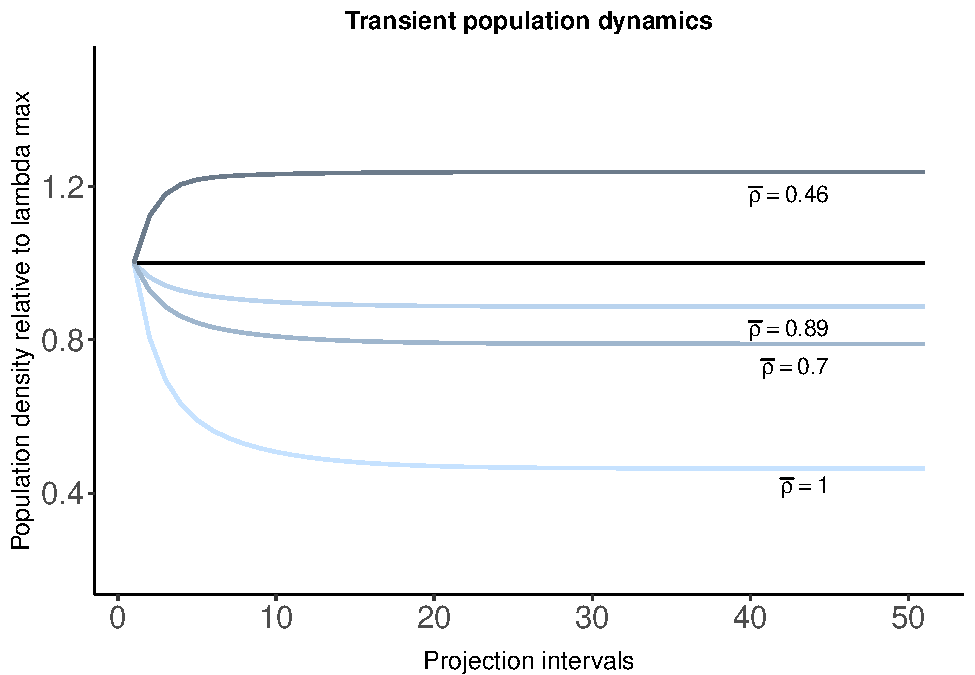
\includegraphics{Diagnostico_Poblacional_files/figure-latex/chap10_5-6.pdf}

\chapter{Funciones de Transferencias}\label{funciones-de-transferencias}

Autores: ``Mariana Hernández Apolinar y Paola Portillo Tzompa''

\section{La elasticidad no lineal}\label{la-elasticidad-no-lineal}

La elasticidad no lineal (\citet{hodgson2004methodological}) se refiere a que los analisis de elasticidad (\citet{caswell2000matrix}, \citet{de2000elasticities}) como explicado en el capitulo xx no son estrictamente lineal y que las perturbaciones en una población pueden tener efectos no lineales en las respuestas de los parametros de densidad o indices de crecimientos. Esos cambios no lineales se pueden observar tambien en la dinamica de transiciones. Si las perturbaciones son pequeñas el uso de analisis de elasticidad pudiesen ser aceptable, por consecuencia los efectos no lineales pueden ser ignorados, pero si las perturbaciones son grandes, los efectos no lineales pueden ser importantes y impactar los procesos de dinamica poblacionales. En los analisis de dinamica poblacional estamos interesado a no solamente el crecimiento de la poblacion pero que pudiese pasar si hubiese cambios pequeños y grandes en los parametros de la matriz sobre los indices de crecimiento y densidad poblacional tal como la supervivencia, crecimiento y fecundidad. La elasticidad no lineal es una herramienta que permite evaluar esos cambios que sean por causa naturales tal como variación ambientales (succesión, dezlisamiento de terreno, mortandad de forofito, cambio climatologico), o antropogénicos (extración de individuos o hasta manejo del sitio para promover el crecimiento de la población).

Es importante reconocer que los analisis de elasticidad y sensitividad ignoran los efectos de la dinamica de transiciones y provee una aproximación linear de cambios que muchas veces no son lineales (\citet{stott2012beyond}).

La elasticidad no lineal es una herramienta que permite evaluar esos cambios que sean por causa naturales tal como variación ambientales (succesión, dezlisamiento de terreno, mortandad de forofito, cambio climatologico), o antropogénicos (extración de individuos o hasta manejo del sitio para promover el crecimiento de la población).

\section{Metodología}\label{metodologuxeda}

El método que presentamos aqui es el desarollado por Hodgson y Townley (2004) (\citet{hodgson2004methodological}, \citet{stott2012beyond}), los cuales presentan un método para calcular la elasticidad no lineal. No se discutirá en detalle el método, pero se presentará un ejemplo de como calcular la elasticidad no lineal.

\begin{Shaded}
\begin{Highlighting}[]
\FunctionTok{library}\NormalTok{(popdemo)}
\end{Highlighting}
\end{Shaded}

\section{Ejemplo tradicional}\label{ejemplo-tradicional}

Aqui la matriz de lefkovitch para la planta \emph{Lepanthes rubripetala} (Tremblay et al.~2015) es presentada.

\begin{Shaded}
\begin{Highlighting}[]
\CommentTok{\#Capturar los datos de la matriz para L. rubripetala (Tremblay et al. 2015)}
\NormalTok{Lr1 }\OtherTok{\textless{}{-}} \FunctionTok{matrix}\NormalTok{(}\FunctionTok{c}\NormalTok{(}\FloatTok{0.4324}\NormalTok{, }\DecValTok{0}\NormalTok{,      }\DecValTok{0}\NormalTok{,     }\FloatTok{0.15}\NormalTok{,}
               \FloatTok{0.3784}\NormalTok{, }\FloatTok{0.8459}\NormalTok{, }\DecValTok{0}\NormalTok{,     }\DecValTok{0}\NormalTok{,}
               \DecValTok{0}\NormalTok{,      }\FloatTok{0.0034}\NormalTok{, }\FloatTok{0.7954}\NormalTok{,}\FloatTok{0.2300}\NormalTok{,}
               \DecValTok{0}\NormalTok{,      }\FloatTok{0.0890}\NormalTok{, }\FloatTok{0.1841}\NormalTok{,}\FloatTok{0.7510}\NormalTok{), }\AttributeTok{byrow=}\ConstantTok{TRUE}\NormalTok{,}\AttributeTok{ncol=}\DecValTok{4}\NormalTok{)}

\CommentTok{\#Capturar las categorias de estado}
\NormalTok{estadios }\OtherTok{\textless{}{-}} \FunctionTok{c}\NormalTok{(}\StringTok{"PL"}\NormalTok{, }\StringTok{"J"}\NormalTok{, }\StringTok{"NR"}\NormalTok{, }\StringTok{"AR"}\NormalTok{)}
\FunctionTok{colnames}\NormalTok{(Lr1) }\OtherTok{\textless{}{-}} \FunctionTok{rownames}\NormalTok{(Lr1) }\OtherTok{\textless{}{-}}\NormalTok{ estadios}

\CommentTok{\#Obtener la matriz L. rubripetala }
\NormalTok{Lr1 }\OtherTok{\textless{}{-}} \FunctionTok{matrix}\NormalTok{(Lr1[}\DecValTok{1}\SpecialCharTok{:}\DecValTok{4}\NormalTok{, ], }\AttributeTok{nrow =} \DecValTok{4}\NormalTok{, }\AttributeTok{dimnames =} \FunctionTok{list}\NormalTok{(estadios, estadios))}
\NormalTok{Lr1}
\end{Highlighting}
\end{Shaded}

\begin{verbatim}
##        PL      J     NR    AR
## PL 0.4324 0.0000 0.0000 0.150
## J  0.3784 0.8459 0.0000 0.000
## NR 0.0000 0.0034 0.7954 0.230
## AR 0.0000 0.0890 0.1841 0.751
\end{verbatim}

Aqui la matriz de elasticad calculado anteriormente.

Nota que la suma de todos los elementos de la matriz de elasticidad. Proporcionalmente el cambio de la supervivencia de el estado de Adulto Reproductivo (AR) tiene el mayor impacto sobre la tasa de crecimiento poblacional. Un pequeño cambio resultaria en un cambio de 0.311 en la tasa de crecimiento poblacional. Al contrario una plantula que se queda plantula (estasis) tuviese muy poco impacto en el crecimiento de la población (0.018). Esos cambios son lineales y son validos si las perturbaciones son pequeñas. Recordar que los indices de sensitividad para tansiciones y estasis son en unidades diferentes que los fecundidades.

\begin{Shaded}
\begin{Highlighting}[]
 \CommentTok{\# Matriz de elasticidad}
\NormalTok{elasticidad}\OtherTok{\textless{}{-}} \FunctionTok{round}\NormalTok{(}\FunctionTok{elas}\NormalTok{(Lr1), }\AttributeTok{digit =} \DecValTok{3}\NormalTok{)}

\NormalTok{elasticidad}
\end{Highlighting}
\end{Shaded}

\begin{verbatim}
##       PL     J    NR    AR
## PL 0.018 0.000 0.000 0.023
## J  0.023 0.122 0.000 0.000
## NR 0.000 0.001 0.313 0.083
## AR 0.000 0.023 0.083 0.311
\end{verbatim}

\section{Valor biológico}\label{valor-bioluxf3gico}

\section{Métodos de calculo}\label{muxe9todos-de-calculo}

En el paquete de R \texttt{popdemo} se puede calcular la elasticidad no lineal \emph{transfer function} con la función \textbf{tfam\_lambda} y \textbf{tfam\_inertia}. La función \textbf{tfam\_lambda} calcula la elasticidad no lineal.

La función \textbf{tfam\_lambda} calcula la elasticidad no lineal de la matriz de edad o de etapas de cada elemento de la matriz A que no sean 0 (zero). Esa función es practica para vizualizar como las perturbaciones en las transiciones del ciclo de vida impacto lambda y observar la no-linealidad de los efectos.

De las 10 transiciones , estasis o fecundidad, 9 tienen un efecto no lineal sobre lambda. Nota primero que el rango de los ejes de ``x'' (efecto de perturbaciones) y la ``y'' el crecimiento porblacional intrinsico varia por cada grafico. La transición de plantula a plantula tiene efecto no lineal sobre lambda bastante pronunciado (primer cuadro a la izquierda primera fila). Se observa que aumentar la proporción de individuos que se quedan en esta etapa no tiene mucho efecto hasta que la perturbación aumenta de ± .5, y despues el efecto es bastante consistente.

La transición de juvenil a no reproductivo tiene un efecto no lineal sobre lambda. La transición de juvenil a adulto reproductivo tiene un efecto no lineal sobre lambda. La transición de no reproductivo a adulto reproductivo tiene un efecto no lineal

\begin{Shaded}
\begin{Highlighting}[]
\NormalTok{n0 }\OtherTok{\textless{}{-}} \FunctionTok{c}\NormalTok{(}\DecValTok{0}\NormalTok{, }\DecValTok{46}\NormalTok{, }\DecValTok{38}\NormalTok{, }\DecValTok{82}\NormalTok{)}

\NormalTok{tfmat\_lamb}\OtherTok{=}\FunctionTok{tfam\_lambda}\NormalTok{(Lr1)}

\FunctionTok{plot}\NormalTok{(tfmat\_lamb)}
\end{Highlighting}
\end{Shaded}

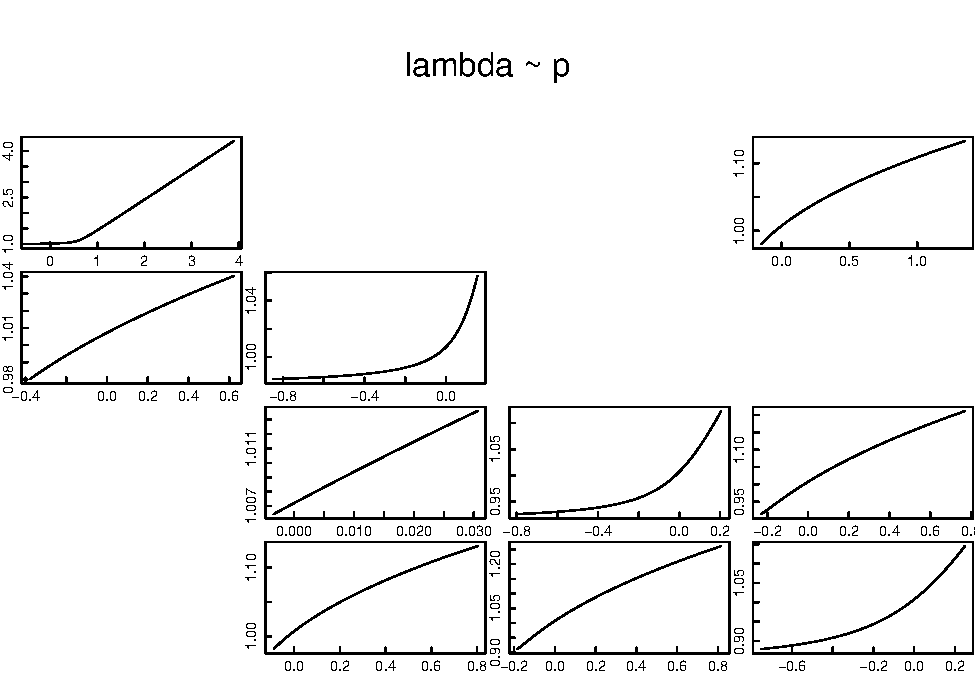
\includegraphics{Diagnostico_Poblacional_files/figure-latex/unnamed-chunk-20-1.pdf}

sens1=sens(Lr1){[}1,1{]}
sens1

abline(eigs(Lr1, ``lambda''), sens1, lty=2)

La función \textbf{tfam\_inertia} calcula la cuan grande o pequeña una población que no este a su equilibro estable puede ser perturbada por consecuencia de dinamica de transiciones. Stott y colegas (\citet{stott2012beyond}) presentan no solamente que el efecto de perturbaciones no es lineal sobre el cambio en lambda pero tambien sobre la inertia, entonces el efecto que tiene sobre poblaciones que no esten a su equilibrio estable.

Usamos la misma temrinalogía de Stott (\citet{stott2012beyond}) para calcular el efecto de elasticidad sobre la inertia de la matriz de \emph{L. rubripetala}. Se evalua el efecto del basado en la estructura del vector de estado inicial. En otra palabra si la cantidad de individuos se encuentra en un estado especifico. El ``upper'' seria los individuos en la etapa mayor (en este caso los adultos reproductivos), el ``lower'' en la estapa menor (en las plantulas) y una estructura de población en al inicio del estudio.

Para evaluar el efecto de no lineal de

\begin{Shaded}
\begin{Highlighting}[]
\NormalTok{n0 }\OtherTok{\textless{}{-}} \FunctionTok{c}\NormalTok{(}\DecValTok{0}\NormalTok{, }\DecValTok{46}\NormalTok{, }\DecValTok{38}\NormalTok{, }\DecValTok{82}\NormalTok{)}

\NormalTok{tf2}\OtherTok{\textless{}{-}}\FunctionTok{tfa\_inertia}\NormalTok{(Lr1, }\AttributeTok{vector=}\NormalTok{n0, }\AttributeTok{d=}\FunctionTok{c}\NormalTok{(}\DecValTok{0}\NormalTok{,}\DecValTok{0}\NormalTok{,}\DecValTok{0}\NormalTok{,}\DecValTok{1}\NormalTok{), }\AttributeTok{e=}\FunctionTok{c}\NormalTok{(}\DecValTok{0}\NormalTok{,}\DecValTok{0}\NormalTok{,}\DecValTok{1}\NormalTok{,}\DecValTok{1}\NormalTok{), }\AttributeTok{prange=}\FunctionTok{seq}\NormalTok{(}\SpecialCharTok{{-}}\FloatTok{0.18}\NormalTok{,}\FloatTok{0.02}\NormalTok{,}\FloatTok{0.01}\NormalTok{))}
\FunctionTok{plot}\NormalTok{(tf2,}\AttributeTok{ylim=}\FunctionTok{c}\NormalTok{(}\DecValTok{0}\NormalTok{, }\DecValTok{2}\NormalTok{),}\AttributeTok{main=}\StringTok{"Population inertia"}\NormalTok{,}\AttributeTok{cex.axis=}\FloatTok{1.4}\NormalTok{,}\AttributeTok{cex.lab=}\FloatTok{1.5}\NormalTok{)}
\NormalTok{inertia}\OtherTok{\textless{}{-}}\FunctionTok{inertia}\NormalTok{(Lr1, }\AttributeTok{vector=}\NormalTok{n0)}
\NormalTok{sens2}\OtherTok{\textless{}{-}}\FunctionTok{tfs\_inertia}\NormalTok{(Lr1, }\AttributeTok{vector=}\NormalTok{n0, }\AttributeTok{d=}\FunctionTok{c}\NormalTok{(}\DecValTok{0}\NormalTok{,}\DecValTok{0}\NormalTok{,}\DecValTok{0}\NormalTok{,}\DecValTok{1}\NormalTok{), }\AttributeTok{e=}\FunctionTok{c}\NormalTok{(}\DecValTok{0}\NormalTok{,}\DecValTok{0}\NormalTok{,}\DecValTok{1}\NormalTok{,}\DecValTok{1}\NormalTok{), }\AttributeTok{tolerance=}\FloatTok{1e{-}5}\NormalTok{)}
\FunctionTok{abline}\NormalTok{(inertia, sens2, }\AttributeTok{lty=}\DecValTok{2}\NormalTok{, }\AttributeTok{col=}\StringTok{"red"}\NormalTok{)}
\end{Highlighting}
\end{Shaded}

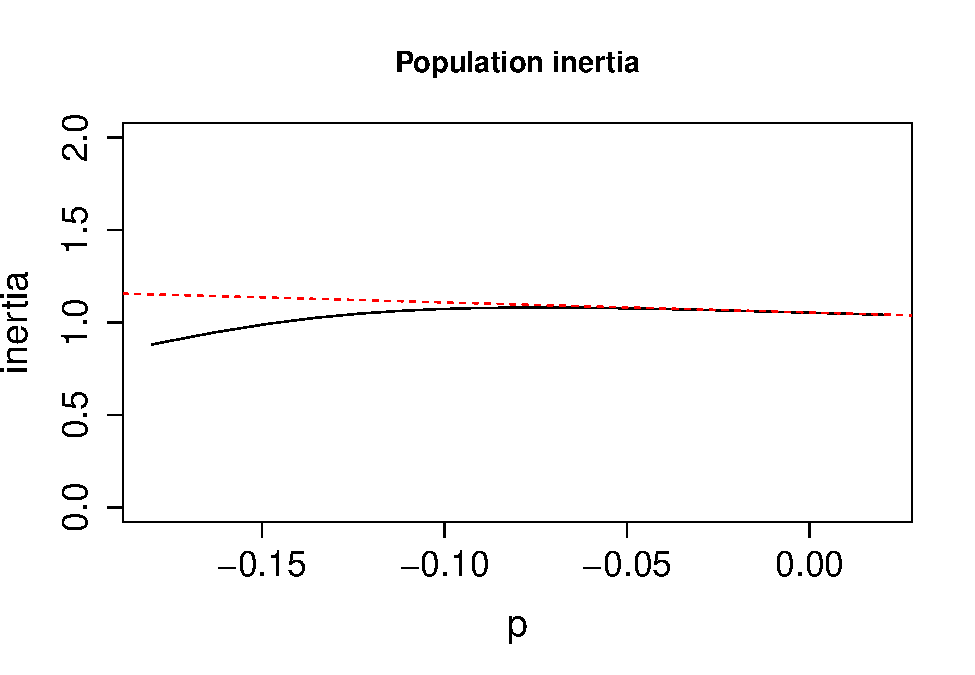
\includegraphics{Diagnostico_Poblacional_files/figure-latex/unnamed-chunk-21-1.pdf}

\begin{Shaded}
\begin{Highlighting}[]
\NormalTok{n0 }\OtherTok{\textless{}{-}} \FunctionTok{c}\NormalTok{(}\DecValTok{0}\NormalTok{, }\DecValTok{46}\NormalTok{, }\DecValTok{38}\NormalTok{, }\DecValTok{82}\NormalTok{)}

\NormalTok{tfmatU}\OtherTok{=}\FunctionTok{tfam\_inertia}\NormalTok{(Lr1, }\AttributeTok{bound =} \StringTok{"upper"}\NormalTok{)}
\NormalTok{tfmat\_I}\OtherTok{=}\FunctionTok{tfam\_inertia}\NormalTok{(Lr1, }\AttributeTok{vector =}\NormalTok{ n0)}
\NormalTok{tfmatL}\OtherTok{=}\FunctionTok{tfam\_inertia}\NormalTok{(Lr1, }\AttributeTok{bound =} \StringTok{"lower"}\NormalTok{)}
\FunctionTok{plot}\NormalTok{(tfmatU)}
\end{Highlighting}
\end{Shaded}

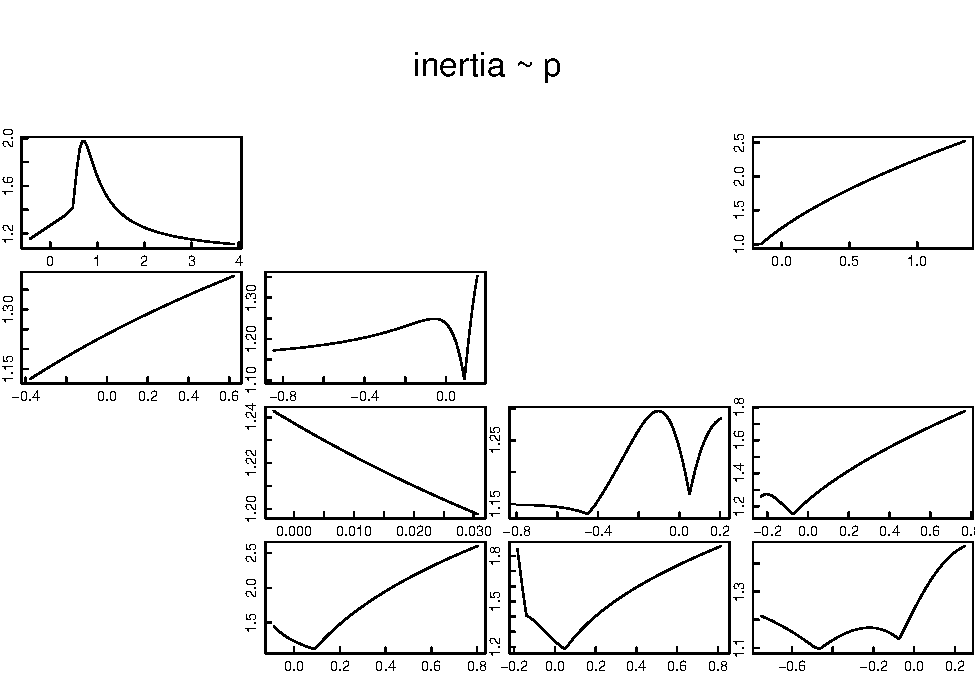
\includegraphics{Diagnostico_Poblacional_files/figure-latex/unnamed-chunk-22-1.pdf}

\begin{Shaded}
\begin{Highlighting}[]
\FunctionTok{plot}\NormalTok{(tfmat\_I)}
\end{Highlighting}
\end{Shaded}

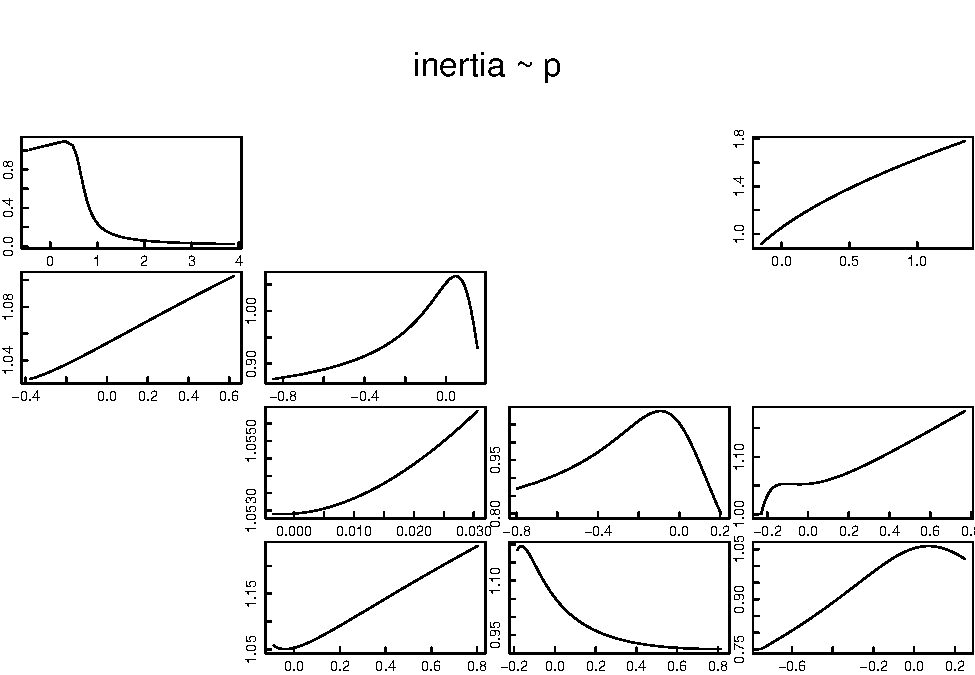
\includegraphics{Diagnostico_Poblacional_files/figure-latex/unnamed-chunk-22-2.pdf}

\begin{Shaded}
\begin{Highlighting}[]
\FunctionTok{plot}\NormalTok{(tfmatL)}
\end{Highlighting}
\end{Shaded}

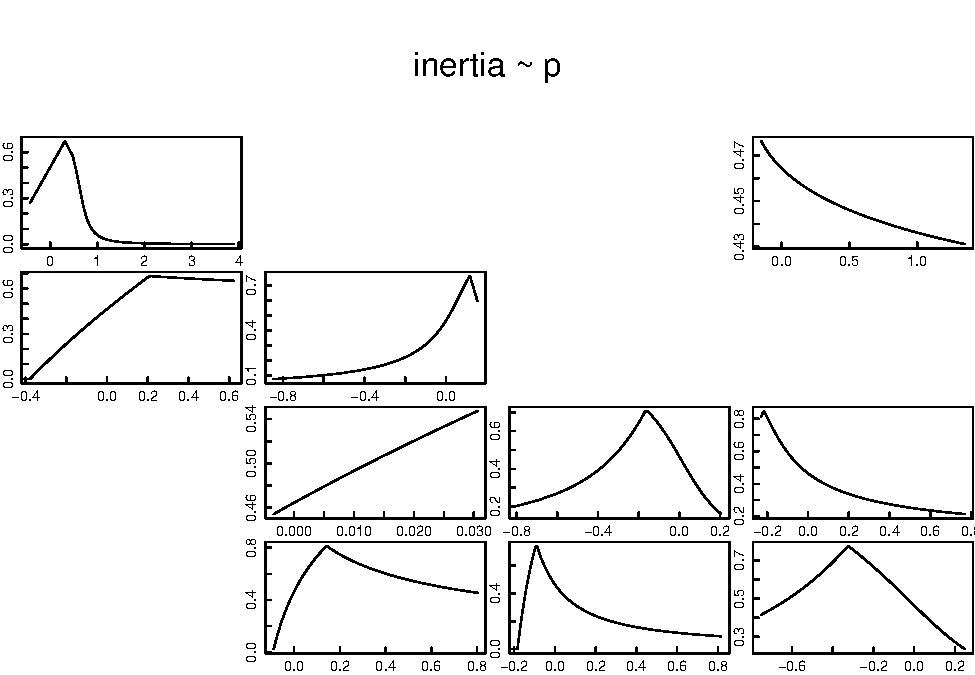
\includegraphics{Diagnostico_Poblacional_files/figure-latex/unnamed-chunk-22-3.pdf}

\section{Paquete de R para calcular le eslaticidad no lineal}\label{paquete-de-r-para-calcular-le-eslaticidad-no-lineal}

\section{Referencias}\label{referencias-3}

\emph{Índices de transferencia}. Con el fin de evaluar en el corto plazo qué cambios cuantitativos habría en la población como respuesta ante una perturbación determinada, se calculan los límites de la dinámica transitoria a través de los \emph{Índices de transferencia}, que incluyen los siguiente tres parámetros (Stoot et al.~2012):

\begin{enumerate}
\def\labelenumi{\alph{enumi})}
\item
  \emph{Reactividad alta y Reactividad baja} (Upper reactivity y Lower reactivity) que representan el crecimiento o el decremento inmediato (i.e.~primer intervalo de tiempo) de la población antes de alcanzar la tasa constante de crecimiento poblacional.
\item
  \emph{Máxima amplificación/Máxima atenuación} (Maximum amplification/Maximum attenuation) que indican,respectivamente, el incremento o decremento máximo futuro del crecimiento poblacional previo a alcanzar la tasa constante de crecimiento poblacional.
\item
  \emph{Inercia alta e Inercia baja} (Upper inertia y Lower inertia) que evalúan el límite más alto o el más bajo en el crecimiento de la población antes de alcanzar la tasa constante de crecimiento poblacional, respectivamente.
\end{enumerate}

\section{Funciones de transferencia}\label{funciones-de-transferencia}

Finalmente, el cálculo de las funciones de transferencia representa el último paso en análisis de dinámica transitoria establecido por Stott y colaboradores (2012). A través de estas ecuaciones se evalúa la elasticidad o efecto de la perturbación sobre la dinámica poblacional. A diferencia de las matrices de elasticidad de los modelos de proyección poblacional, estas elasticidades no son lineales y evidencian la importancia relativa de la de la perturbación en la categoría de tamaño/estado sobre el crecimiento de la población en el corto plazo. Estas ecuaciones también están disponibles en el programa \emph{Popdemo} de \emph{R} y sus resultados se representan a través de gráficas.

La perturbación de la estructura está determinada ppor dos vectores \emph{d} y \emph{e}

\begin{Shaded}
\begin{Highlighting}[]
\DocumentationTok{\#\#PASO 6: ANALISIS DE LAS FUNCIONES DE TRANSFERENCIA }
\CommentTok{\#Establecer márgenes:}
\CommentTok{\#Vector original}
\FunctionTok{library}\NormalTok{(popdemo)}

\NormalTok{nLr0 }\OtherTok{\textless{}{-}} \FunctionTok{c}\NormalTok{(}\DecValTok{0}\NormalTok{, }\DecValTok{46}\NormalTok{, }\DecValTok{38}\NormalTok{, }\DecValTok{82}\NormalTok{)}

\CommentTok{\#PERTURBACIÓN DEL VECTOR ORIGINAL}

\CommentTok{\#1) Entrada de la matriz a(1,1): plántulas a plántulas}
\NormalTok{tf1 }\OtherTok{\textless{}{-}} \FunctionTok{tfa\_lambda}\NormalTok{(Lr1, }\AttributeTok{d =} \FunctionTok{c}\NormalTok{(}\DecValTok{1}\NormalTok{, }\DecValTok{0}\NormalTok{, }\DecValTok{0}\NormalTok{, }\DecValTok{0}\NormalTok{),}
                  \AttributeTok{e =} \FunctionTok{c}\NormalTok{(}\DecValTok{1}\NormalTok{, }\DecValTok{0}\NormalTok{, }\DecValTok{0}\NormalTok{, }\DecValTok{0}\NormalTok{),}
                  \AttributeTok{prange =} \FunctionTok{seq}\NormalTok{(}\DecValTok{0}\NormalTok{, }\DecValTok{4}\NormalTok{, }\FloatTok{0.01}\NormalTok{))}

\CommentTok{\#Gráfica de la dinámica poblacional}
\FunctionTok{plot}\NormalTok{(tf1, }\AttributeTok{ann =} \ConstantTok{FALSE}\NormalTok{)}
\FunctionTok{title}\NormalTok{(}\AttributeTok{main =} \StringTok{"Dinámica poblacional (Plántulas {-} Plántulas)"}\NormalTok{, }\AttributeTok{ylab =} \StringTok{"Lambda"}\NormalTok{, }\AttributeTok{xlab =} \StringTok{"p"}\NormalTok{)}

\CommentTok{\#Cálculo de lambda{-}max:}
\NormalTok{lambda1 }\OtherTok{\textless{}{-}} \FunctionTok{Re}\NormalTok{(}\FunctionTok{eigen}\NormalTok{(Lr1)}\SpecialCharTok{$}\NormalTok{values[}\DecValTok{1}\NormalTok{]) }

\CommentTok{\#Cálculo de la sensibilidad }
\NormalTok{sens1 }\OtherTok{\textless{}{-}} \FunctionTok{tfs\_lambda}\NormalTok{(Lr1, }\AttributeTok{d =} \FunctionTok{c}\NormalTok{(}\DecValTok{1}\NormalTok{, }\DecValTok{0}\NormalTok{, }\DecValTok{0}\NormalTok{, }\DecValTok{0}\NormalTok{), }\AttributeTok{e =} \FunctionTok{c}\NormalTok{(}\DecValTok{1}\NormalTok{, }\DecValTok{0}\NormalTok{, }\DecValTok{0}\NormalTok{, }\DecValTok{0}\NormalTok{))}

\CommentTok{\#Agregar la línea, especificando el intercepto y la pendiente}
\FunctionTok{abline}\NormalTok{(lambda1, sens1, }\AttributeTok{lty =} \DecValTok{2}\NormalTok{, }\AttributeTok{col =} \StringTok{"red"}\NormalTok{)}
\end{Highlighting}
\end{Shaded}

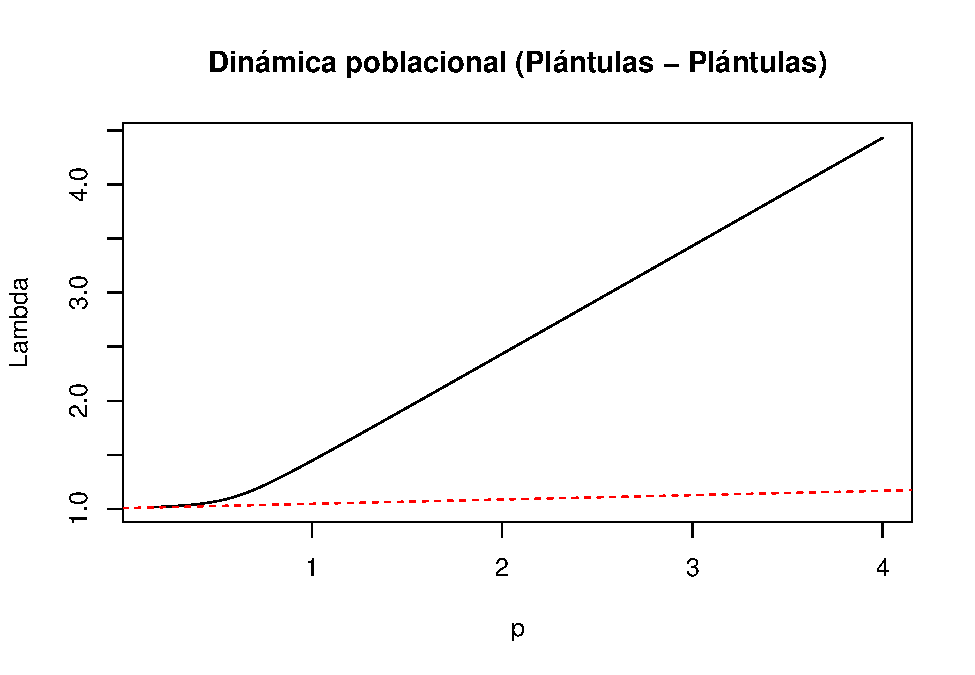
\includegraphics{Diagnostico_Poblacional_files/figure-latex/chap10_6-1.pdf}

\begin{Shaded}
\begin{Highlighting}[]
\CommentTok{\#2) Entrada de la matriz a(2,1): plántulas y juveniles}
\NormalTok{tf2 }\OtherTok{\textless{}{-}} \FunctionTok{tfa\_lambda}\NormalTok{(Lr1, }\AttributeTok{d =} \FunctionTok{c}\NormalTok{(}\DecValTok{0}\NormalTok{, }\DecValTok{1}\NormalTok{, }\DecValTok{0}\NormalTok{, }\DecValTok{0}\NormalTok{),}
                  \AttributeTok{e =} \FunctionTok{c}\NormalTok{(}\DecValTok{1}\NormalTok{, }\DecValTok{0}\NormalTok{, }\DecValTok{0}\NormalTok{, }\DecValTok{0}\NormalTok{),}
                  \AttributeTok{prange =} \FunctionTok{seq}\NormalTok{(}\SpecialCharTok{{-}}\FloatTok{0.4}\NormalTok{, }\FloatTok{0.6}\NormalTok{, }\FloatTok{0.01}\NormalTok{))}

\CommentTok{\#Gráfica de la dinámica poblacional}
\FunctionTok{plot}\NormalTok{(tf2, }\AttributeTok{ann =} \ConstantTok{FALSE}\NormalTok{)}
\FunctionTok{title}\NormalTok{(}\AttributeTok{main =} \StringTok{"Dinámica poblacional (Plántulas {-} Juveniles)"}\NormalTok{, }\AttributeTok{ylab =} \StringTok{"Lambda"}\NormalTok{, }\AttributeTok{xlab =} \StringTok{"p"}\NormalTok{)}

\CommentTok{\#Cálculo de lambda{-}max:}
\NormalTok{lambda2 }\OtherTok{\textless{}{-}} \FunctionTok{Re}\NormalTok{(}\FunctionTok{eigen}\NormalTok{(Lr1)}\SpecialCharTok{$}\NormalTok{values[}\DecValTok{1}\NormalTok{]) }

\CommentTok{\#Cálculo de la sensibilidad }
\NormalTok{sens2 }\OtherTok{\textless{}{-}} \FunctionTok{tfs\_lambda}\NormalTok{(Lr1, }\AttributeTok{d =} \FunctionTok{c}\NormalTok{(}\DecValTok{0}\NormalTok{, }\DecValTok{1}\NormalTok{, }\DecValTok{0}\NormalTok{, }\DecValTok{0}\NormalTok{), }\AttributeTok{e =} \FunctionTok{c}\NormalTok{(}\DecValTok{1}\NormalTok{, }\DecValTok{0}\NormalTok{, }\DecValTok{0}\NormalTok{, }\DecValTok{0}\NormalTok{))}

\CommentTok{\#Agregar la línea, especificando el intercepto y la pendiente}
\FunctionTok{abline}\NormalTok{(lambda2, sens2, }\AttributeTok{lty =} \DecValTok{2}\NormalTok{, }\AttributeTok{col =} \StringTok{"red"}\NormalTok{)}
\end{Highlighting}
\end{Shaded}

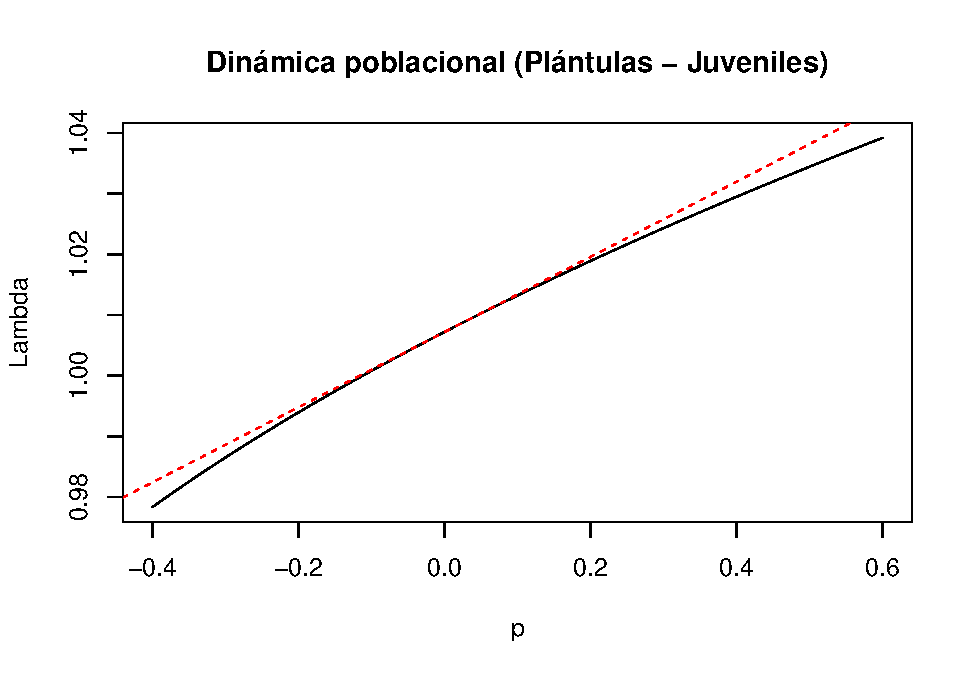
\includegraphics{Diagnostico_Poblacional_files/figure-latex/chap10_6-2.pdf}

\begin{Shaded}
\begin{Highlighting}[]
\CommentTok{\#3) Entrada de la matriz a(2,2): juveniles y juveniles}
\NormalTok{tf3 }\OtherTok{\textless{}{-}} \FunctionTok{tfa\_lambda}\NormalTok{(Lr1, }\AttributeTok{d =} \FunctionTok{c}\NormalTok{(}\DecValTok{0}\NormalTok{, }\DecValTok{1}\NormalTok{, }\DecValTok{0}\NormalTok{, }\DecValTok{0}\NormalTok{),}
                  \AttributeTok{e =} \FunctionTok{c}\NormalTok{(}\DecValTok{0}\NormalTok{, }\DecValTok{1}\NormalTok{, }\DecValTok{0}\NormalTok{, }\DecValTok{0}\NormalTok{),}
                  \AttributeTok{prange =} \FunctionTok{seq}\NormalTok{(}\SpecialCharTok{{-}}\FloatTok{0.8}\NormalTok{, }\FloatTok{0.1}\NormalTok{, }\FloatTok{0.001}\NormalTok{))}

\CommentTok{\#Gráfica de la dinámica poblacional}
\FunctionTok{plot}\NormalTok{(tf3, }\AttributeTok{ann =} \ConstantTok{FALSE}\NormalTok{)}
\FunctionTok{title}\NormalTok{(}\AttributeTok{main =} \StringTok{"Dinámica poblacional (Juveniles {-} Juveniles)"}\NormalTok{, }\AttributeTok{ylab =} \StringTok{"Lambda"}\NormalTok{, }\AttributeTok{xlab =} \StringTok{"p"}\NormalTok{)}

\CommentTok{\#Cálculo de lambda{-}max:}
\NormalTok{lambda3 }\OtherTok{\textless{}{-}} \FunctionTok{Re}\NormalTok{(}\FunctionTok{eigen}\NormalTok{(Lr1)}\SpecialCharTok{$}\NormalTok{values[}\DecValTok{1}\NormalTok{]) }

\CommentTok{\#Cálculo de la sensibilidad }
\NormalTok{sens3 }\OtherTok{\textless{}{-}} \FunctionTok{tfs\_lambda}\NormalTok{(Lr1, }\AttributeTok{d =} \FunctionTok{c}\NormalTok{(}\DecValTok{0}\NormalTok{, }\DecValTok{1}\NormalTok{, }\DecValTok{0}\NormalTok{, }\DecValTok{0}\NormalTok{), }\AttributeTok{e =} \FunctionTok{c}\NormalTok{(}\DecValTok{0}\NormalTok{, }\DecValTok{1}\NormalTok{, }\DecValTok{0}\NormalTok{, }\DecValTok{0}\NormalTok{))}

\CommentTok{\#Agregar la línea, especificando el intercepto y la pendiente}
\FunctionTok{abline}\NormalTok{(lambda3, sens3, }\AttributeTok{lty =} \DecValTok{2}\NormalTok{, }\AttributeTok{col =} \StringTok{"red"}\NormalTok{)}
\end{Highlighting}
\end{Shaded}

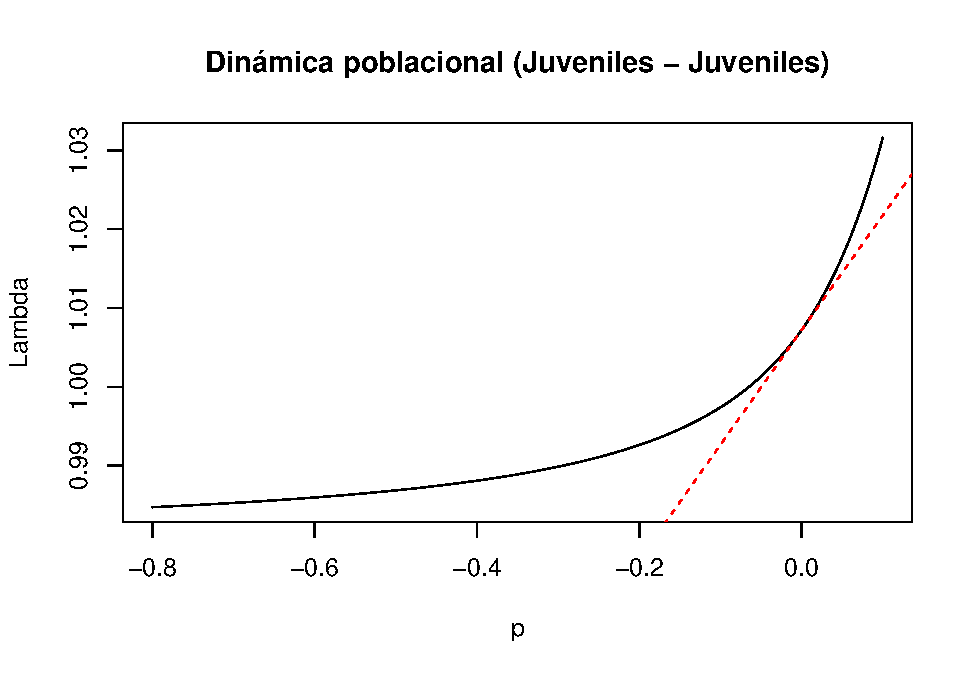
\includegraphics{Diagnostico_Poblacional_files/figure-latex/chap10_6-3.pdf}

\begin{Shaded}
\begin{Highlighting}[]
\CommentTok{\#4) Entrada de la matriz a(3,2): juveniles y no reproductivos}
\NormalTok{tf4 }\OtherTok{\textless{}{-}} \FunctionTok{tfa\_lambda}\NormalTok{(Lr1, }\AttributeTok{d =} \FunctionTok{c}\NormalTok{(}\DecValTok{0}\NormalTok{, }\DecValTok{0}\NormalTok{, }\DecValTok{1}\NormalTok{, }\DecValTok{0}\NormalTok{),}
                  \AttributeTok{e =} \FunctionTok{c}\NormalTok{(}\DecValTok{0}\NormalTok{, }\DecValTok{1}\NormalTok{, }\DecValTok{0}\NormalTok{, }\DecValTok{0}\NormalTok{),}
                  \AttributeTok{prange =} \FunctionTok{seq}\NormalTok{(}\SpecialCharTok{{-}}\FloatTok{0.001}\NormalTok{, }\FloatTok{0.03}\NormalTok{, }\FloatTok{0.01}\NormalTok{))}

\CommentTok{\#Gráfica de la dinámica poblacional}
\FunctionTok{plot}\NormalTok{(tf4, }\AttributeTok{ann =} \ConstantTok{FALSE}\NormalTok{)}
\FunctionTok{title}\NormalTok{(}\AttributeTok{main =} \StringTok{"Dinámica poblacional (Juveniles {-} No reproductivos)"}\NormalTok{, }\AttributeTok{ylab =} \StringTok{"Lambda"}\NormalTok{, }\AttributeTok{xlab =} \StringTok{"p"}\NormalTok{)}

\CommentTok{\#Cálculo de lambda{-}max:}
\NormalTok{lambda4 }\OtherTok{\textless{}{-}} \FunctionTok{Re}\NormalTok{(}\FunctionTok{eigen}\NormalTok{(Lr1)}\SpecialCharTok{$}\NormalTok{values[}\DecValTok{1}\NormalTok{]) }

\CommentTok{\#Cálculo de la sensibilidad}
\NormalTok{sens4 }\OtherTok{\textless{}{-}} \FunctionTok{tfs\_lambda}\NormalTok{(Lr1, }\AttributeTok{d =} \FunctionTok{c}\NormalTok{(}\DecValTok{0}\NormalTok{,}\DecValTok{0}\NormalTok{,}\DecValTok{1}\NormalTok{,}\DecValTok{0}\NormalTok{), }\AttributeTok{e =} \FunctionTok{c}\NormalTok{(}\DecValTok{0}\NormalTok{, }\DecValTok{1}\NormalTok{, }\DecValTok{0}\NormalTok{, }\DecValTok{0}\NormalTok{))}

\CommentTok{\#Agregar la línea, especificando el intercepto y la pendiente}
\FunctionTok{abline}\NormalTok{(lambda4, sens4, }\AttributeTok{lty =} \DecValTok{2}\NormalTok{, }\AttributeTok{col =} \StringTok{"red"}\NormalTok{)}
\end{Highlighting}
\end{Shaded}

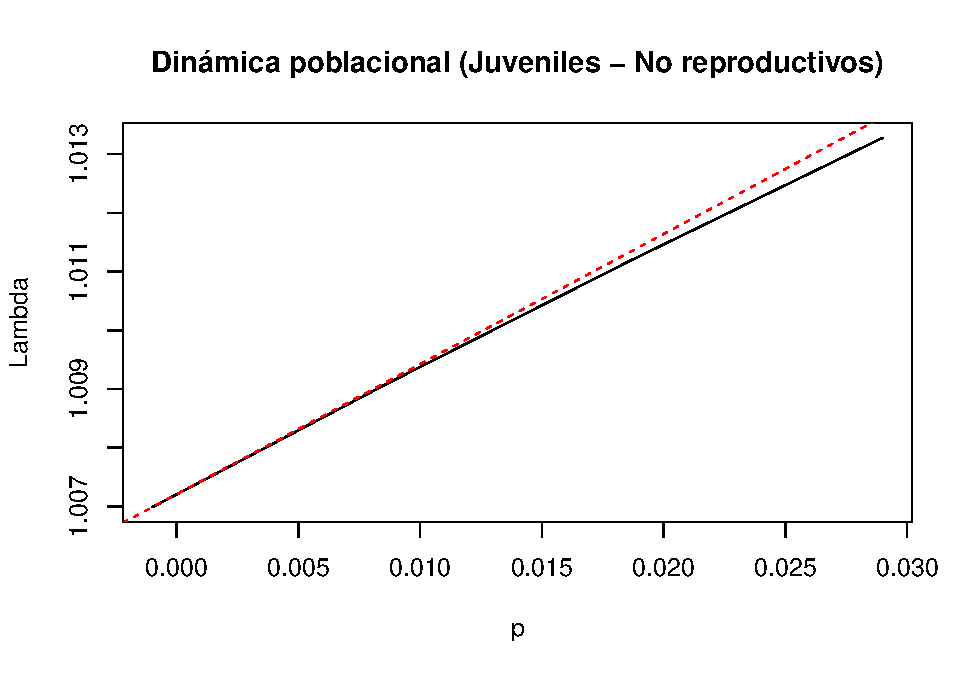
\includegraphics{Diagnostico_Poblacional_files/figure-latex/chap10_6-4.pdf}

\begin{Shaded}
\begin{Highlighting}[]
\CommentTok{\#5) Entrada de la matriz a(4,2): juveniles a adultos}
\NormalTok{tf5 }\OtherTok{\textless{}{-}} \FunctionTok{tfa\_lambda}\NormalTok{(Lr1, }\AttributeTok{d =} \FunctionTok{c}\NormalTok{(}\DecValTok{0}\NormalTok{,}\DecValTok{0}\NormalTok{,}\DecValTok{0}\NormalTok{,}\DecValTok{1}\NormalTok{),}
                  \AttributeTok{e =} \FunctionTok{c}\NormalTok{(}\DecValTok{0}\NormalTok{,}\DecValTok{1}\NormalTok{,}\DecValTok{0}\NormalTok{,}\DecValTok{0}\NormalTok{),}
                  \AttributeTok{prange =} \FunctionTok{seq}\NormalTok{(}\DecValTok{0}\NormalTok{,}\FloatTok{0.8}\NormalTok{,}\FloatTok{0.01}\NormalTok{))}

\CommentTok{\#Gráfica de la dinámica poblacional}
\FunctionTok{plot}\NormalTok{(tf5, }\AttributeTok{ann =} \ConstantTok{FALSE}\NormalTok{)}
\FunctionTok{title}\NormalTok{(}\AttributeTok{main =} \StringTok{"Dinámica poblacional (Juveniles {-} Adultos)"}\NormalTok{, }\AttributeTok{ylab =} \StringTok{"Lambda"}\NormalTok{, }\AttributeTok{xlab =} \StringTok{"p"}\NormalTok{)}

\CommentTok{\#Cálculo de lambda{-}max:}
\NormalTok{lambda5 }\OtherTok{\textless{}{-}} \FunctionTok{Re}\NormalTok{(}\FunctionTok{eigen}\NormalTok{(Lr1)}\SpecialCharTok{$}\NormalTok{values[}\DecValTok{1}\NormalTok{]) }

\CommentTok{\#Cálculo de la sensibilidad}
\NormalTok{sens5 }\OtherTok{\textless{}{-}} \FunctionTok{tfs\_lambda}\NormalTok{(Lr1, }\AttributeTok{d =} \FunctionTok{c}\NormalTok{(}\DecValTok{0}\NormalTok{, }\DecValTok{0}\NormalTok{, }\DecValTok{0}\NormalTok{, }\DecValTok{1}\NormalTok{), }\AttributeTok{e =} \FunctionTok{c}\NormalTok{(}\DecValTok{0}\NormalTok{, }\DecValTok{1}\NormalTok{, }\DecValTok{0}\NormalTok{, }\DecValTok{0}\NormalTok{))}

\CommentTok{\#Agregar la línea, especificando el intercepto y la pendiente}
\FunctionTok{abline}\NormalTok{(lambda5, sens5, }\AttributeTok{lty =} \DecValTok{2}\NormalTok{, }\AttributeTok{col =} \StringTok{"red"}\NormalTok{)}
\end{Highlighting}
\end{Shaded}

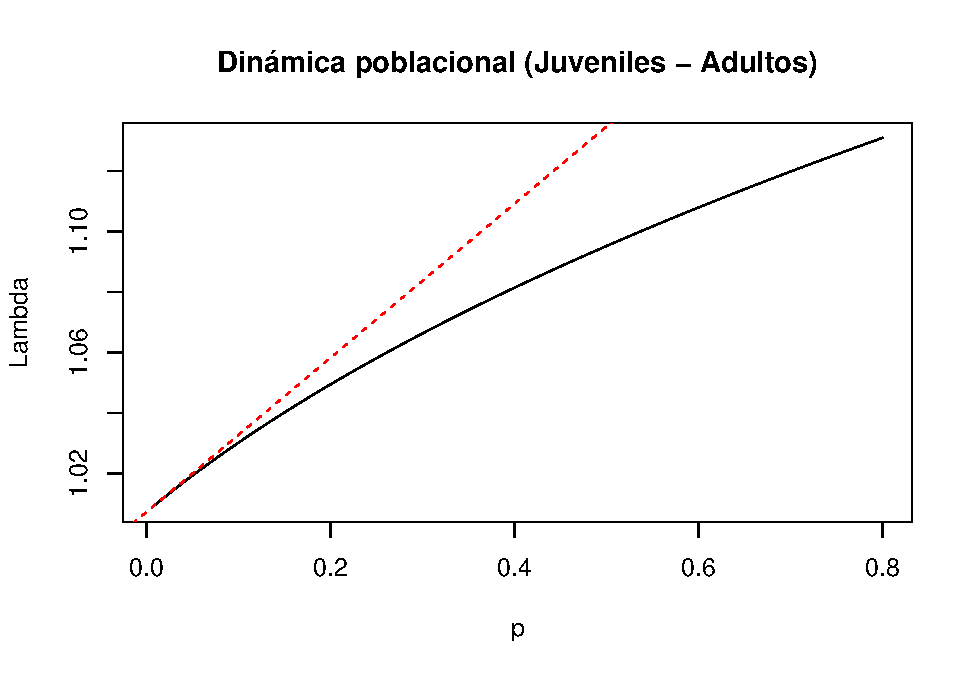
\includegraphics{Diagnostico_Poblacional_files/figure-latex/chap10_6-5.pdf}

\begin{Shaded}
\begin{Highlighting}[]
\CommentTok{\#6) Entrada de la matriz a(3,3): adultos no reproductivos a adultos no reproductivos}
\NormalTok{tf6 }\OtherTok{\textless{}{-}} \FunctionTok{tfa\_lambda}\NormalTok{(Lr1, }\AttributeTok{d =} \FunctionTok{c}\NormalTok{(}\DecValTok{0}\NormalTok{, }\DecValTok{0}\NormalTok{, }\DecValTok{1}\NormalTok{, }\DecValTok{0}\NormalTok{),}
                  \AttributeTok{e =} \FunctionTok{c}\NormalTok{(}\DecValTok{0}\NormalTok{, }\DecValTok{0}\NormalTok{, }\DecValTok{1}\NormalTok{, }\DecValTok{0}\NormalTok{),}
                  \AttributeTok{prange =} \FunctionTok{seq}\NormalTok{(}\SpecialCharTok{{-}}\FloatTok{0.8}\NormalTok{, }\FloatTok{0.2}\NormalTok{, }\FloatTok{0.01}\NormalTok{))}

\CommentTok{\#Gráfica de la dinámica poblacional}
\FunctionTok{plot}\NormalTok{(tf6, }\AttributeTok{ann =} \ConstantTok{FALSE}\NormalTok{)}
\FunctionTok{title}\NormalTok{(}\AttributeTok{main =} \StringTok{"Dinámica poblacional (Adultos No rep {-} Adultos  No reproductivos)"}\NormalTok{, }\AttributeTok{ylab =} \StringTok{"Lambda"}\NormalTok{, }\AttributeTok{xlab =} \StringTok{"p"}\NormalTok{)}

\CommentTok{\#Cálculo de lambda{-}max:}
\NormalTok{lambda6 }\OtherTok{\textless{}{-}} \FunctionTok{Re}\NormalTok{(}\FunctionTok{eigen}\NormalTok{(Lr1)}\SpecialCharTok{$}\NormalTok{values[}\DecValTok{1}\NormalTok{]) }

\CommentTok{\#Cálculo de la sensibilidad}
\NormalTok{sens6 }\OtherTok{\textless{}{-}} \FunctionTok{tfs\_lambda}\NormalTok{(Lr1, }\AttributeTok{d =} \FunctionTok{c}\NormalTok{(}\DecValTok{0}\NormalTok{,}\DecValTok{0}\NormalTok{,}\DecValTok{0}\NormalTok{,}\DecValTok{1}\NormalTok{), }\AttributeTok{e =} \FunctionTok{c}\NormalTok{(}\DecValTok{0}\NormalTok{,}\DecValTok{1}\NormalTok{,}\DecValTok{0}\NormalTok{,}\DecValTok{0}\NormalTok{))}

\CommentTok{\#Agregar la línea, especificando el intercepto y la pendiente}
\FunctionTok{abline}\NormalTok{(lambda6, sens6, }\AttributeTok{lty =} \DecValTok{2}\NormalTok{, }\AttributeTok{col =} \StringTok{"red"}\NormalTok{)}
\end{Highlighting}
\end{Shaded}

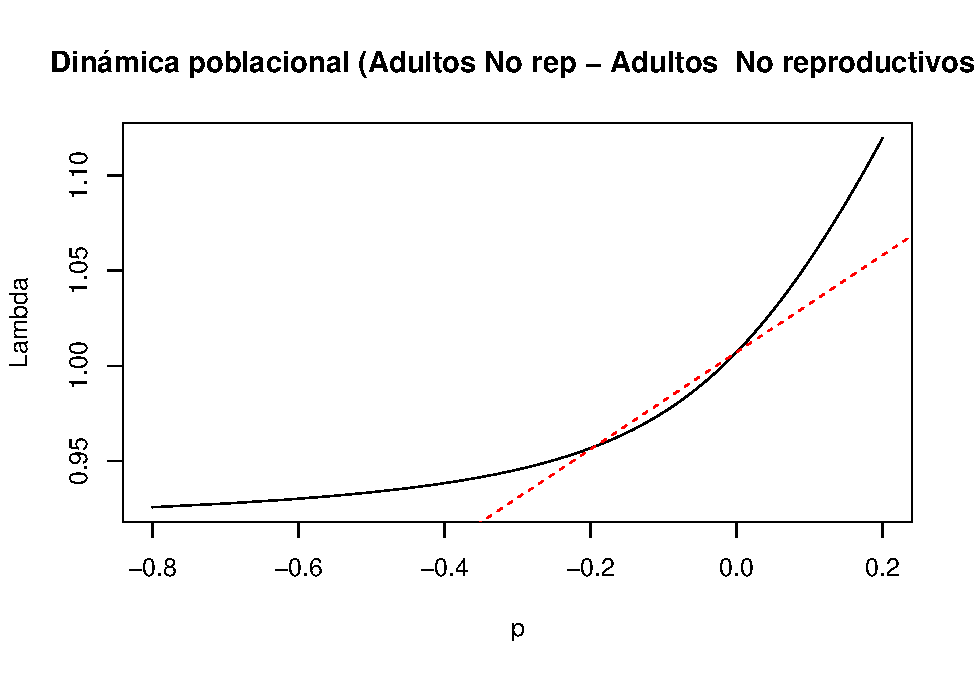
\includegraphics{Diagnostico_Poblacional_files/figure-latex/chap10_6-6.pdf}

\begin{Shaded}
\begin{Highlighting}[]
\CommentTok{\#7) Entrada de la matriz a(4,3): adultos no reproductivos a adultos reproductivos}

\NormalTok{tf7 }\OtherTok{\textless{}{-}} \FunctionTok{tfa\_lambda}\NormalTok{(Lr1, }\AttributeTok{d =} \FunctionTok{c}\NormalTok{(}\DecValTok{0}\NormalTok{,}\DecValTok{0}\NormalTok{,}\DecValTok{0}\NormalTok{,}\DecValTok{1}\NormalTok{),}
                  \AttributeTok{e =} \FunctionTok{c}\NormalTok{(}\DecValTok{0}\NormalTok{,}\DecValTok{0}\NormalTok{,}\DecValTok{1}\NormalTok{,}\DecValTok{0}\NormalTok{),}
                  \AttributeTok{prange =} \FunctionTok{seq}\NormalTok{(}\SpecialCharTok{{-}}\FloatTok{0.2}\NormalTok{,}\FloatTok{0.8}\NormalTok{,}\FloatTok{0.001}\NormalTok{))}

\CommentTok{\#Gráfica de la dinámica poblacional}
\FunctionTok{plot}\NormalTok{(tf7, }\AttributeTok{ann =} \ConstantTok{FALSE}\NormalTok{)}
\FunctionTok{title}\NormalTok{(}\AttributeTok{main =} \StringTok{"Dinámica poblacional (Adultos No rep {-} Adultos No rep)"}\NormalTok{, }\AttributeTok{ylab =} \StringTok{"Lambda"}\NormalTok{, }\AttributeTok{xlab =} \StringTok{"p"}\NormalTok{)}

\CommentTok{\#Cálculo de lambda{-}max:}
\NormalTok{lambda7 }\OtherTok{\textless{}{-}} \FunctionTok{Re}\NormalTok{(}\FunctionTok{eigen}\NormalTok{(Lr1)}\SpecialCharTok{$}\NormalTok{values[}\DecValTok{1}\NormalTok{]) }

\CommentTok{\#Cálculo de la sensibilidad}
\NormalTok{sens7 }\OtherTok{\textless{}{-}} \FunctionTok{tfs\_lambda}\NormalTok{(Lr1, }\AttributeTok{d =} \FunctionTok{c}\NormalTok{(}\DecValTok{0}\NormalTok{,}\DecValTok{0}\NormalTok{,}\DecValTok{0}\NormalTok{,}\DecValTok{1}\NormalTok{), }\AttributeTok{e =} \FunctionTok{c}\NormalTok{(}\DecValTok{0}\NormalTok{,}\DecValTok{0}\NormalTok{,}\DecValTok{1}\NormalTok{,}\DecValTok{0}\NormalTok{))}

\CommentTok{\#Agregar la línea, especificando el intercepto y la pendiente}
\FunctionTok{abline}\NormalTok{(lambda7, sens7, }\AttributeTok{lty =} \DecValTok{2}\NormalTok{, }\AttributeTok{col =} \StringTok{"red"}\NormalTok{)}
\end{Highlighting}
\end{Shaded}

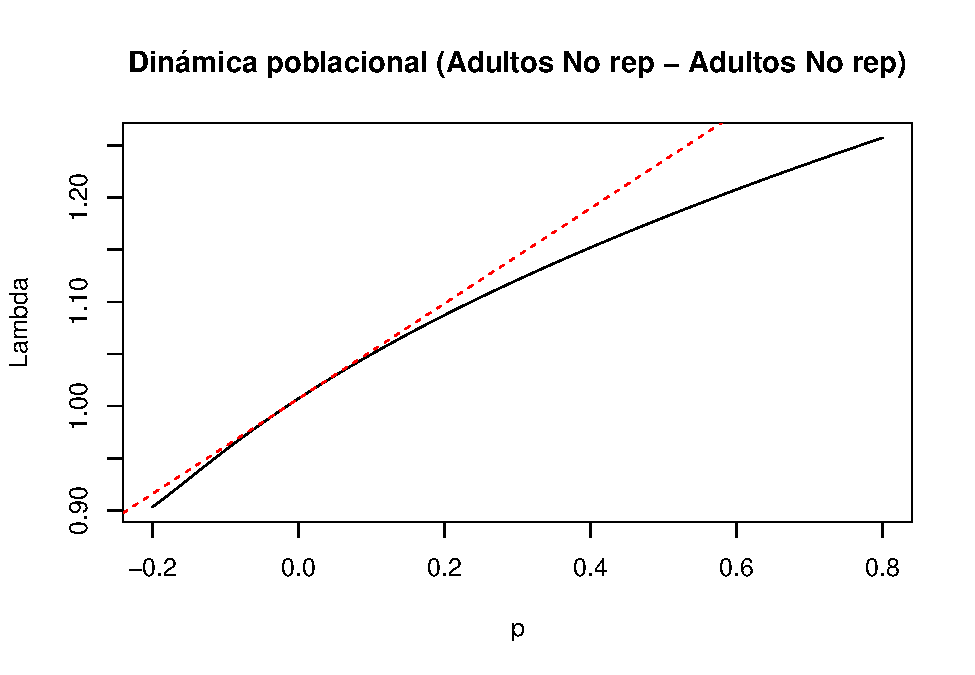
\includegraphics{Diagnostico_Poblacional_files/figure-latex/chap10_6-7.pdf}

\begin{Shaded}
\begin{Highlighting}[]
\CommentTok{\#8) Entrada de la matriz a(1,4): adultos reproductivos a plántulas}

\NormalTok{tf8 }\OtherTok{\textless{}{-}} \FunctionTok{tfa\_lambda}\NormalTok{(Lr1, }\AttributeTok{d =} \FunctionTok{c}\NormalTok{(}\DecValTok{1}\NormalTok{,}\DecValTok{0}\NormalTok{,}\DecValTok{0}\NormalTok{,}\DecValTok{0}\NormalTok{),}
                  \AttributeTok{e =} \FunctionTok{c}\NormalTok{(}\DecValTok{0}\NormalTok{,}\DecValTok{0}\NormalTok{,}\DecValTok{0}\NormalTok{,}\DecValTok{1}\NormalTok{),}
                  \AttributeTok{prange =} \FunctionTok{seq}\NormalTok{(}\SpecialCharTok{{-}}\FloatTok{0.2}\NormalTok{,}\FloatTok{0.8}\NormalTok{,}\FloatTok{0.001}\NormalTok{))}

\CommentTok{\#Gráfica de la dinámica poblacional}
\FunctionTok{plot}\NormalTok{(tf8, }\AttributeTok{ann =} \ConstantTok{FALSE}\NormalTok{)}
\FunctionTok{title}\NormalTok{(}\AttributeTok{main =} \StringTok{"Dinámica poblacional (Adultos reproductivos {-} Plántulas)"}\NormalTok{, }\AttributeTok{ylab =} \StringTok{"Lambda"}\NormalTok{, }\AttributeTok{xlab =} \StringTok{"p"}\NormalTok{)}

\CommentTok{\#Cálculo de lambda{-}max:}
\NormalTok{lambda8 }\OtherTok{\textless{}{-}} \FunctionTok{Re}\NormalTok{(}\FunctionTok{eigen}\NormalTok{(Lr1)}\SpecialCharTok{$}\NormalTok{values[}\DecValTok{1}\NormalTok{]) }

\CommentTok{\#Cálculo de la sensibilidad}
\NormalTok{sens8 }\OtherTok{\textless{}{-}} \FunctionTok{tfs\_lambda}\NormalTok{(Lr1, }\AttributeTok{d =} \FunctionTok{c}\NormalTok{(}\DecValTok{1}\NormalTok{,}\DecValTok{0}\NormalTok{,}\DecValTok{0}\NormalTok{,}\DecValTok{0}\NormalTok{), }\AttributeTok{e =} \FunctionTok{c}\NormalTok{(}\DecValTok{0}\NormalTok{,}\DecValTok{0}\NormalTok{,}\DecValTok{0}\NormalTok{,}\DecValTok{1}\NormalTok{))}

\CommentTok{\#Agregar la línea, especificando el intercepto y la pendiente}
\FunctionTok{abline}\NormalTok{(lambda8, sens8, }\AttributeTok{lty =} \DecValTok{2}\NormalTok{, }\AttributeTok{col =} \StringTok{"red"}\NormalTok{)}
\end{Highlighting}
\end{Shaded}

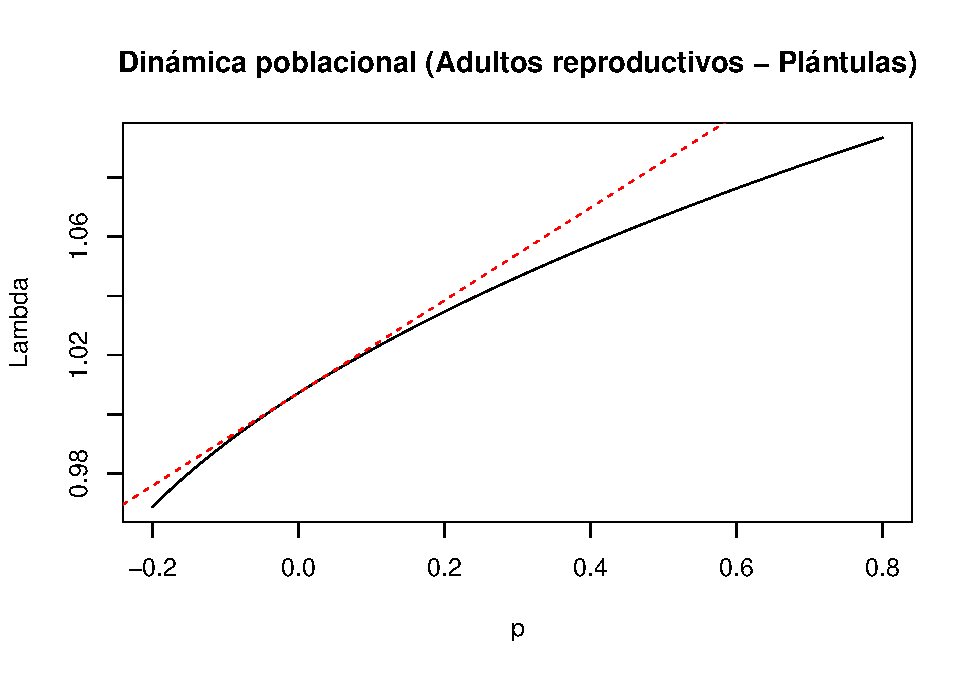
\includegraphics{Diagnostico_Poblacional_files/figure-latex/chap10_6-8.pdf}

\begin{Shaded}
\begin{Highlighting}[]
\CommentTok{\#9) Entrada de la matriz a(3,4): adultos reproductivos a plántulas}

\NormalTok{tf9 }\OtherTok{\textless{}{-}} \FunctionTok{tfa\_lambda}\NormalTok{(Lr1, }\AttributeTok{d =} \FunctionTok{c}\NormalTok{(}\DecValTok{0}\NormalTok{, }\DecValTok{0}\NormalTok{,}\DecValTok{1}\NormalTok{, }\DecValTok{0}\NormalTok{),}
                  \AttributeTok{e =} \FunctionTok{c}\NormalTok{(}\DecValTok{0}\NormalTok{, }\DecValTok{0}\NormalTok{, }\DecValTok{0}\NormalTok{,}\DecValTok{1}\NormalTok{),}
                  \AttributeTok{prange =} \FunctionTok{seq}\NormalTok{(}\SpecialCharTok{{-}}\FloatTok{0.2}\NormalTok{, }\FloatTok{0.8}\NormalTok{, }\FloatTok{0.001}\NormalTok{))}

\CommentTok{\#Gráfica de la dinámica poblacional}
\FunctionTok{plot}\NormalTok{(tf9, }\AttributeTok{ann =} \ConstantTok{FALSE}\NormalTok{)}
\FunctionTok{title}\NormalTok{(}\AttributeTok{main =} \StringTok{"Dinámica poblacional (Adultos reproductivos {-} Plántulas)"}\NormalTok{, }\AttributeTok{ylab =} \StringTok{"Lambda"}\NormalTok{, }\AttributeTok{xlab =} \StringTok{"p"}\NormalTok{)}

\CommentTok{\#Cálculo de lambda{-}max:}
\NormalTok{lambda9 }\OtherTok{\textless{}{-}} \FunctionTok{Re}\NormalTok{(}\FunctionTok{eigen}\NormalTok{(Lr1)}\SpecialCharTok{$}\NormalTok{values[}\DecValTok{1}\NormalTok{]) }

\CommentTok{\#Cálculo de la sensibilidad}
\NormalTok{sens9 }\OtherTok{\textless{}{-}} \FunctionTok{tfs\_lambda}\NormalTok{(Lr1, }\AttributeTok{d =} \FunctionTok{c}\NormalTok{(}\DecValTok{0}\NormalTok{, }\DecValTok{0}\NormalTok{, }\DecValTok{0}\NormalTok{,}\DecValTok{1}\NormalTok{), }\AttributeTok{e =} \FunctionTok{c}\NormalTok{(}\DecValTok{0}\NormalTok{, }\DecValTok{0}\NormalTok{, }\DecValTok{1}\NormalTok{, }\DecValTok{0}\NormalTok{))}

\CommentTok{\#Agregar la línea, especificando el intercepto y la pendiente}
\FunctionTok{abline}\NormalTok{(lambda9, sens9, }\AttributeTok{lty =} \DecValTok{2}\NormalTok{, }\AttributeTok{col =} \StringTok{"red"}\NormalTok{)}
\end{Highlighting}
\end{Shaded}

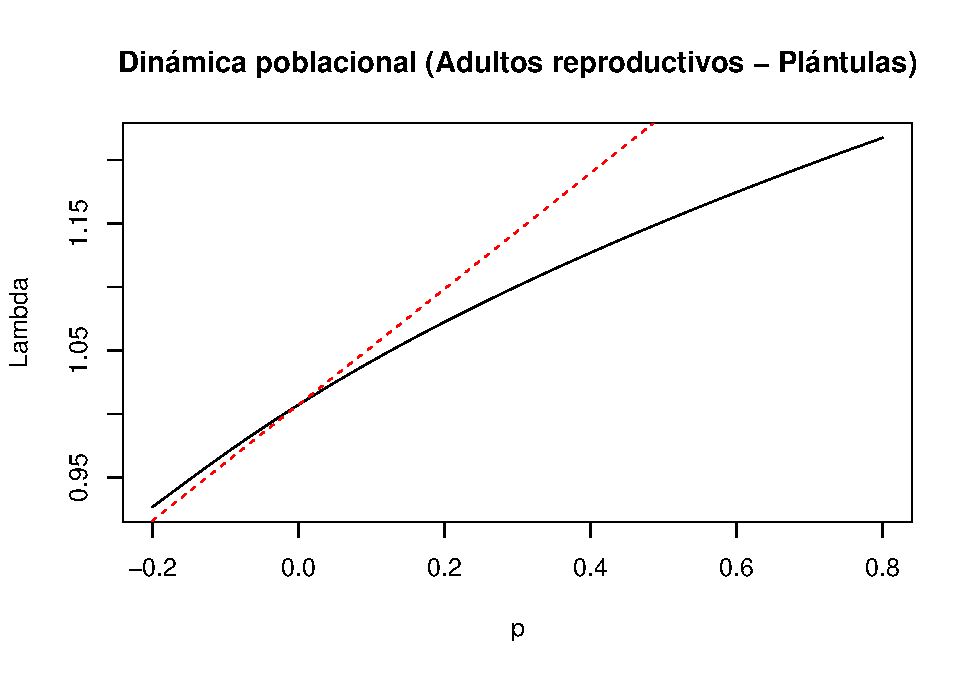
\includegraphics{Diagnostico_Poblacional_files/figure-latex/chap10_6-9.pdf}

\begin{Shaded}
\begin{Highlighting}[]
\CommentTok{\#10) Entrada de la matriz a(4,4): adultos reproductivos a adultos reproductivos}

\NormalTok{tf10 }\OtherTok{\textless{}{-}} \FunctionTok{tfa\_lambda}\NormalTok{(Lr1, }\AttributeTok{d =} \FunctionTok{c}\NormalTok{(}\DecValTok{0}\NormalTok{, }\DecValTok{0}\NormalTok{, }\DecValTok{0}\NormalTok{, }\DecValTok{1}\NormalTok{),}
                  \AttributeTok{e =} \FunctionTok{c}\NormalTok{(}\DecValTok{0}\NormalTok{, }\DecValTok{0}\NormalTok{, }\DecValTok{0}\NormalTok{, }\DecValTok{1}\NormalTok{),}
                  \AttributeTok{prange =} \FunctionTok{seq}\NormalTok{(}\SpecialCharTok{{-}}\FloatTok{0.6}\NormalTok{, }\FloatTok{0.2}\NormalTok{, }\FloatTok{0.001}\NormalTok{))}

\CommentTok{\#Gráfica de la dinámica poblacional}
\FunctionTok{plot}\NormalTok{(tf10, }\AttributeTok{ann =} \ConstantTok{FALSE}\NormalTok{)}
\FunctionTok{title}\NormalTok{(}\AttributeTok{main =} \StringTok{"Dinámica poblacional (Adultos rep {-} Adultos rep)"}\NormalTok{, }\AttributeTok{ylab =} \StringTok{"Lambda"}\NormalTok{, }\AttributeTok{xlab =} \StringTok{"p"}\NormalTok{)}

\CommentTok{\#Cálculo de lambda{-}max:}
\NormalTok{lambda10 }\OtherTok{\textless{}{-}} \FunctionTok{Re}\NormalTok{(}\FunctionTok{eigen}\NormalTok{(Lr1)}\SpecialCharTok{$}\NormalTok{values[}\DecValTok{1}\NormalTok{]) }

\CommentTok{\#Cálculo de la sensibilidad}
\NormalTok{sens10 }\OtherTok{\textless{}{-}} \FunctionTok{tfs\_lambda}\NormalTok{(Lr1, }\AttributeTok{d =} \FunctionTok{c}\NormalTok{(}\DecValTok{0}\NormalTok{,}\DecValTok{0}\NormalTok{,}\DecValTok{0}\NormalTok{,}\DecValTok{1}\NormalTok{), }\AttributeTok{e =} \FunctionTok{c}\NormalTok{(}\DecValTok{0}\NormalTok{,}\DecValTok{0}\NormalTok{,}\DecValTok{0}\NormalTok{,}\DecValTok{1}\NormalTok{))}

\CommentTok{\#Agregar la línea, especificando el intercepto y la pendiente}
\FunctionTok{abline}\NormalTok{(lambda10, sens10, }\AttributeTok{lty =} \DecValTok{2}\NormalTok{, }\AttributeTok{col =} \StringTok{"red"}\NormalTok{)}

\CommentTok{\#Definir márgenes}
\FunctionTok{par}\NormalTok{(}\AttributeTok{mfrow =} \FunctionTok{c}\NormalTok{(}\DecValTok{4}\NormalTok{,}\DecValTok{4}\NormalTok{))}
\FunctionTok{par}\NormalTok{(}\AttributeTok{mfg =} \FunctionTok{c}\NormalTok{(}\DecValTok{1}\NormalTok{,}\DecValTok{1}\NormalTok{))}

\CommentTok{\#Gráficas de la función de transferencia de la inercia en el ciclo de vida de L. rubripetala (población 1)}
\NormalTok{tfmatriz }\OtherTok{\textless{}{-}} \FunctionTok{tfam\_inertia}\NormalTok{(Lr1,}\AttributeTok{vector =}\NormalTok{ nLr0)}
\FunctionTok{plot}\NormalTok{(tfmatriz)}
\end{Highlighting}
\end{Shaded}

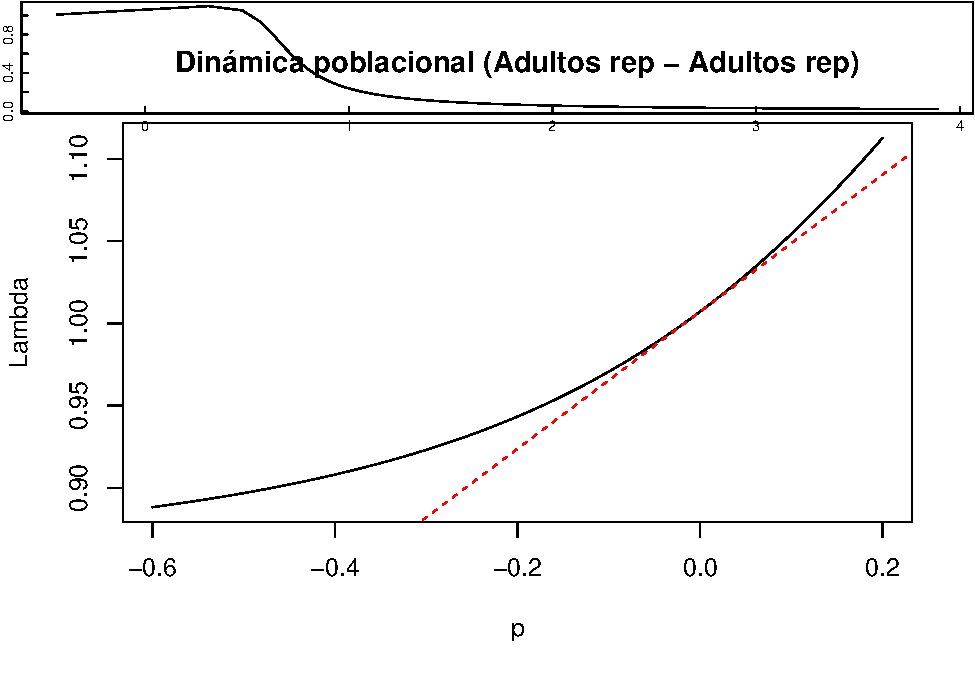
\includegraphics{Diagnostico_Poblacional_files/figure-latex/chap10_6-10.pdf} 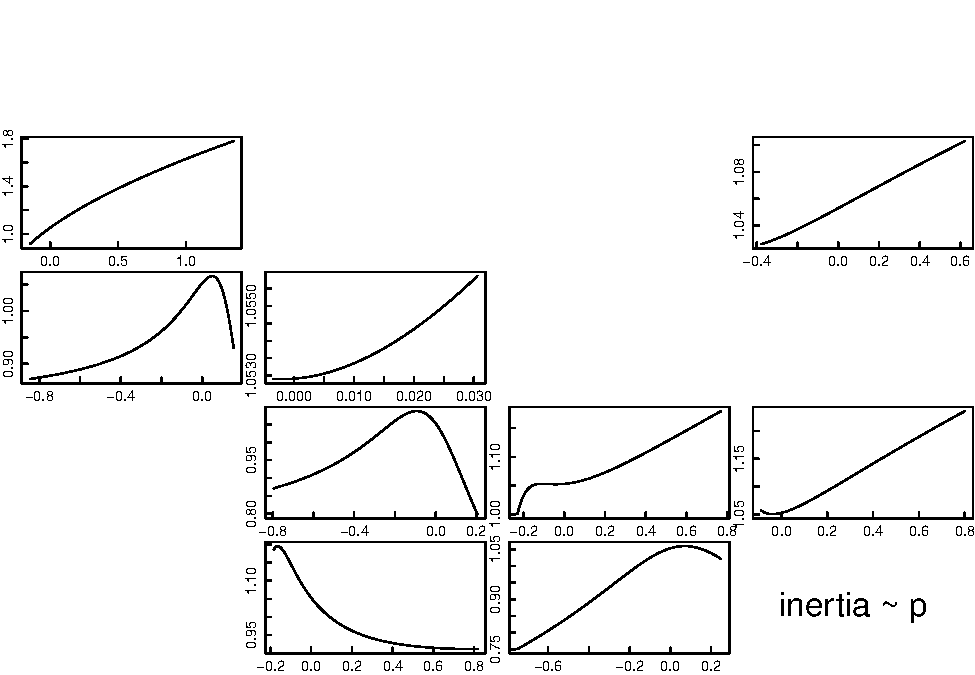
\includegraphics{Diagnostico_Poblacional_files/figure-latex/chap10_6-11.pdf}

Raventós y colaboradores (2015) estimaron el crecimiento poblacional de corto plazo de dos orquídeas epífitas después del paso de un huracán. Dado que a su paso se pierden individuos, se simuló si la reintroducción de plántulas y adultos mitigaban los efectos de este fenómeno en Cuba. Los resultados sugieren que la reintroducción de adultos tiene un efecto positivo sobre

\chapter{LTRE}\label{ltre}

por : Adriana Ramírez-Martínez

\section{Introducción a LTRE}\label{introducciuxf3n-a-ltre}

La variación en las parametros de la historia de vida de una especie y las causas de estas diferencias se puede evaluar a diferentes niveles: genético, demográfico, espacial o temporal. Esta variación en ecología es la norma. La variación se encuentra en todos aspectos desde la parte genética de los individuos que compone una población, la variación ambiental y las interacciones bióticas y abióticas; además de la plasticidad fenotípica que es la interacción entre la genética y el ambiente. ¿Cuál es esa variación? ¿en otra palabra qué es lo que varía? y ¿cómo los individuos responden a las variables bióticas y abióticas? son aspectos importantes para determinar la ecología, evolución y conservación de las especies. La causa de la variación en una población se puede resumir a tres componentes principales, la genética, el efecto del ambiente y la interacción entre ambiente y genética (plasticidad fenotípica) (\citet{hastings2021effects}; \citet{sun2019multivariate}). Dentro de un contexto de dinámica poblacional las condiciones que los individuos en las poblaciones experimentan varían, ya sea durante tratamientos manipulados, localidades o periodos de tiempo, y por consecuencia los datos que colectamos con diferencias en espacio/tiempo también varían y pudieran tener efecto sobre la matriz de proyección poblacional \textbf{A}. Por tanto, las entradas (los parámetros) de esa matriz A variarán en tiempo/espacio o experimento y esto tendría un impacto sobre la tasa de crecimiento poblacional (λ) y su dispersión en los estimados (Intervalo de confianza o credibilidad; \citet{caswell2000matrix}, \citet{caswell2010life}).

Tomando en cuenta lo anterior un Experimento de Respuesta de Tabla de Vida (\textbf{ERTV}) conocido también como \emph{Life Table Response Experiment} (LTRE por sus siglas en inglés) descompone la diferencia o varianza en \emph{λ} entre múltiples poblaciones o tiempo dentro de las contribuciones de los elementos de la matriz y sus interacciones (\citet{caswell1989analysis}). Entonces al realizar este análisis podemos tener una apreciación de cómo los cambios en la matriz de datos recolectados en diferentes tiempos y espacio impactan las tasas vitales y a su vez que causan cambios en el crecimiento intrínseco \emph{λ} y otros parámetros poblacionales (\citet{caswell1989analysis}, \citet{caswell2010life}).

Desde la aplicación del primer ERTV por Birch (1953) en su estudio sobre el efecto de la temperatura, humedad y el alimento sobre tres especies de escarabajos de harina, las aplicaciones de estos análisis han sido variadas con diversos fines en las últimas dos décadas (\citet{caswell1989analysis}, \citet{caswell2010life}). Tanto en diseños fijos en los que se manipulan uno o más factores, como en diseños aleatorios en los que se analizan parámetros demográficos en condiciones naturales no manipuladas a lo largo del tiempo o del espacio (\citet{horvitz1997relative}; \citet{teitel2016assessing}). Los diseños fijos se han utilizado en poblaciones de animales para investigar las consecuencias demográficas de la exposición a contaminantes, la manipulación del alimento o la manipulación de la densidad poblacional (\citet{hansen1999multiannual}, 1999; \citet{levin1996demographic}; \citet{oli2001effect}). En plantas, los análisis ERTV se han utilizado para evaluar las consecuencias demográficas de la disponibilidad de polinizadores o de la herbívora, competencia, efectos en intensidades de cosecha y de fenómenos naturales e inducidos por el humano (\citet{davison2010demographic}; \citet{gaoue2010effects}; \citet{garcia2002reproductive}; \citet{hart2021simulated}; \citet{jacquemyn2012stochastic}; \citet{miriti2001effects}; \citet{mondragon2009population}; \citet{nordbakken2004demography}; \citet{schmidt2011matrix}).

Los métodos para calcular los ERTV están constantemente actualizándose y de acuerdo con (\citet{hernandez2023exact}) existen 186 análisis de ERTV para 75 especies de animales y 1487 para 200 especies de plantas. Aunque en este trabajo no utilizamos la metodología expuesta por dichos autores mostramos una forma práctica de la aplicación de este análisis.

\subsection{¿Cómo se diferencia la elasticidad de ERTV?}\label{cuxf3mo-se-diferencia-la-elasticidad-de-ertv}

A diferencia de la elasticidad, el cual es un tipo de análisis de perturbación que examina cuánto cambiaría el crecimiento de la población si se cambiaran una de las entradas de la matriz, el análisis ERTV examina cuánto cambió \emph{λ} en función de la variación observada en las entradas de la matriz (\citet{caswell2000matrix}, \citet{caswell2010life}; \citet{horvitz1997relative}); y por consecuencia es un análisis que toma en cuenta el cambio de las variaciones individualmente registradas en matrices en diferentes poblaciones/ tiempo / experimentos, etc. (\citet{caswell2010life}). Nota que ERTV es una herramineta suplementaria para evaluar el efecto de perturbaciones como los de elasticidad, dinámica de transiciones y funciones de transferencias y no un reemplazos. Cada una de estas herramientas tiene un propósito y una interpretación diferente con sus supuestos.

\begin{center}\rule{0.5\linewidth}{0.5pt}\end{center}

\section{Métodos}\label{muxe9todos-1}

\subsection{Ejemplo práctico de ERTV}\label{ejemplo-pruxe1ctico-de-ertv}

Para ejemplificar el cálculo de los ERTV utilizaremos los datos recabados por Ramírez-Martínez colectados de a 2017-2018 para la orquídea epífita \emph{Oncidium brachyandrum} Lindl. en un bosque de encino estacional en Oaxaca, México (\citet{ramirez2021host}). La pregunta principal del estudio era saber qué tasas vitales estaban ligadas a las variaciones en los valores de λ de poblaciones de \emph{O. brachyandrum} creciendo sobre los hospederos \emph{Quercus martinezii} C.H.Mull. y \emph{Q. rugosa} Née. Usando el método ERTV se pudo evaluar el efecto que tiene la variación observada en los parámetros de las matrices en función de las especies de hospedero en los que se encontraban creciendo.

Como el ERTV es una forma de análisis retrospectivo y es análogo al ANOVA (porque cuantifica los efectos observados de los elementos individuales de matriz sobre la variación observada en \emph{λ}, en contraposición a los efectos esperados) se requiere de un valor de referencia para realizar las comparaciones, por lo que se toma la matriz con el valor más alto de \emph{λ} como valor de referencia (\citet{caswell2010life}; \citet{timsina2021six}).

A continuación, se muestran dos matrices de tipo Lefkovitch (matrices contruidas a base de estadíos) para las poblaciones de \emph{O. brachyandrum} y sus valores respectivos de λ en los dos hospederos, \emph{Q. martinezii} (λ=1.3; I.C: 1.11-1.45) y \emph{Q. rugosa} (λ=0.98; I.C: 0.87-0.99) (Cuadro 1). Notamos claramente que el valor de λ era mayor en \emph{Q. martinezii} por lo que la matriz de esta especie fue la matriz de referencia para calcular los ERTV.

\begin{center}\rule{0.5\linewidth}{0.5pt}\end{center}

\subsection{Matrices de proyecciones y ciclo de vida por especie de hospedero}\label{matrices-de-proyecciones-y-ciclo-de-vida-por-especie-de-hospedero}

Cuadro 1. Matrices de proyección poblaciones de dos poblaciones de \emph{Oncidiun brachyandrum} creciendo sobre \emph{Quercus martinezii} y \emph{Q. rugosa}. Los valores de λ (intervalos de confianza ± 95\%) son mostrados en la parte superior izquierda de cada matriz. \emph{qx}, mortalidad por estadío; \emph{w}, categorías estables de tamaño por estadío; valor reproductivo por estadío, \emph{n} = el tamaño de muestra en el tiempo cero (el primer muestreo). p: plántula, i: infantil, j: juvenil, A; adulto (\citet{ramirez2021host}). Los valores en negritas son los valores que representan la proporción de individuos que se queda en ese estadio.

\includegraphics{Figures/imagen1.jpg}

\begin{center}\rule{0.5\linewidth}{0.5pt}\end{center}

\subsection{Diagrama del ciclo de vida}\label{diagrama-del-ciclo-de-vida}

\subsection{\texorpdfstring{Diagrama para \emph{Quercus martinezii}}{Diagrama para Quercus martinezii}}\label{diagrama-para-quercus-martinezii}

Primeramente se creó el ciclo de vida por especie de hospedero utilizando el siguiente código:

\begin{Shaded}
\begin{Highlighting}[]
\FunctionTok{library}\NormalTok{(Rage)}
\FunctionTok{library}\NormalTok{(DiagrammeR)}


\NormalTok{matmart }\OtherTok{\textless{}{-}} \FunctionTok{rbind}\NormalTok{(}
  \FunctionTok{c}\NormalTok{(}\FloatTok{0.68}\NormalTok{, }\FloatTok{0.02}\NormalTok{, }\FloatTok{3.88}\NormalTok{, }\FloatTok{16.53}\NormalTok{),}
  \FunctionTok{c}\NormalTok{(}\FloatTok{0.22}\NormalTok{, }\FloatTok{0.76}\NormalTok{, }\FloatTok{0.23}\NormalTok{, }\FloatTok{0.0}\NormalTok{),}
  \FunctionTok{c}\NormalTok{(}\FloatTok{0.0}\NormalTok{, }\FloatTok{0.13}\NormalTok{, }\FloatTok{0.53}\NormalTok{, }\FloatTok{0.58}\NormalTok{),}
  \FunctionTok{c}\NormalTok{(}\FloatTok{0.0}\NormalTok{, }\FloatTok{0.0}\NormalTok{, }\FloatTok{0.17}\NormalTok{, }\FloatTok{0.38}\NormalTok{))}

\NormalTok{stages }\OtherTok{\textless{}{-}} \FunctionTok{c}\NormalTok{(}\StringTok{"plántula"}\NormalTok{, }\StringTok{"infantil"}\NormalTok{, }\StringTok{"juvenil"}\NormalTok{, }\StringTok{"adulto"}\NormalTok{)}
\NormalTok{title }\OtherTok{\textless{}{-}} \ConstantTok{NULL}
\NormalTok{graph }\OtherTok{\textless{}{-}} \FunctionTok{expand.grid}\NormalTok{(}\AttributeTok{to =}\NormalTok{ stages, }\AttributeTok{from =}\NormalTok{ stages)}
\NormalTok{graph}\SpecialCharTok{$}\NormalTok{trans }\OtherTok{\textless{}{-}} \FunctionTok{round}\NormalTok{(}\FunctionTok{c}\NormalTok{(matmart), }\DecValTok{4}\NormalTok{)}
\NormalTok{graph }\OtherTok{\textless{}{-}}\NormalTok{ graph[graph}\SpecialCharTok{$}\NormalTok{trans }\SpecialCharTok{\textgreater{}} \DecValTok{0}\NormalTok{, ]}
\NormalTok{nodes }\OtherTok{\textless{}{-}} \FunctionTok{paste}\NormalTok{(}\FunctionTok{paste0}\NormalTok{(}\StringTok{"\textquotesingle{}"}\NormalTok{, stages, }\StringTok{"\textquotesingle{}"}\NormalTok{), }\AttributeTok{collapse =} \StringTok{"; "}\NormalTok{)}
\NormalTok{graph}\SpecialCharTok{$}\NormalTok{min\_len }\OtherTok{\textless{}{-}}\NormalTok{ (}\FunctionTok{as.numeric}\NormalTok{(graph}\SpecialCharTok{$}\NormalTok{to) }\SpecialCharTok{{-}} \FunctionTok{as.numeric}\NormalTok{(graph}\SpecialCharTok{$}\NormalTok{from)) }\SpecialCharTok{*} \DecValTok{4}
\end{Highlighting}
\end{Shaded}

\includegraphics{Diagnostico_Poblacional_files/figure-latex/unnamed-chunk-23-1.pdf}

\vspace{-5truemm}

Figura x: Ciclo de vida de \emph{Oncidium brachyandrum} creciendo sobre \emph{Quercus martinezii}. Las flechas representan las transiciones entre estadíos, estasis y fecundidades y los números son las tasas vitales de fecundidad, supervivencia y crecimiento. El color \(\color{#ffc125}{\text{amarillo}}\) para fecundidad, \(\color{  #36648b}{\text{azul}}\) para supervivencia y \(\color{#548b54}{\text{verde}}\) para crecimiento, \(\color{#7a378b}{\text{violeta}}\) para retroceso y azul oscuro para permanencia.

\subsection{Diagrama para Quercus rugosa}\label{diagrama-para-quercus-rugosa}

\begin{Shaded}
\begin{Highlighting}[]
\FunctionTok{library}\NormalTok{(Rage)}
\FunctionTok{library}\NormalTok{(DiagrammeR)}

\NormalTok{matrug }\OtherTok{\textless{}{-}} \FunctionTok{rbind}\NormalTok{(}
  \FunctionTok{c}\NormalTok{(}\FloatTok{0.64}\NormalTok{, }\FloatTok{0.06}\NormalTok{, }\DecValTok{0}\NormalTok{, }\FloatTok{0.0045}\NormalTok{),}
  \FunctionTok{c}\NormalTok{(}\FloatTok{0.27}\NormalTok{, }\FloatTok{0.75}\NormalTok{, }\FloatTok{0.27}\NormalTok{, }\FloatTok{0.0}\NormalTok{),}
  \FunctionTok{c}\NormalTok{(}\FloatTok{0.0}\NormalTok{, }\FloatTok{0.08}\NormalTok{, }\FloatTok{0.47}\NormalTok{, }\FloatTok{0.28}\NormalTok{),}
  \FunctionTok{c}\NormalTok{(}\FloatTok{0.0}\NormalTok{, }\FloatTok{0.0}\NormalTok{, }\FloatTok{0.27}\NormalTok{, }\FloatTok{0.68}\NormalTok{))}
\NormalTok{stages }\OtherTok{\textless{}{-}} \FunctionTok{c}\NormalTok{(}\StringTok{"plántula"}\NormalTok{, }\StringTok{"infantil"}\NormalTok{, }\StringTok{"juvenil"}\NormalTok{, }\StringTok{"adulto"}\NormalTok{)}
\NormalTok{title }\OtherTok{\textless{}{-}} \ConstantTok{NULL}
\NormalTok{graph }\OtherTok{\textless{}{-}} \FunctionTok{expand.grid}\NormalTok{(}\AttributeTok{to =}\NormalTok{ stages, }\AttributeTok{from =}\NormalTok{ stages)}
\NormalTok{graph}\SpecialCharTok{$}\NormalTok{trans }\OtherTok{\textless{}{-}} \FunctionTok{round}\NormalTok{(}\FunctionTok{c}\NormalTok{(matrug), }\DecValTok{4}\NormalTok{)}
\NormalTok{graph }\OtherTok{\textless{}{-}}\NormalTok{ graph[graph}\SpecialCharTok{$}\NormalTok{trans }\SpecialCharTok{\textgreater{}} \DecValTok{0}\NormalTok{, ]}
\NormalTok{nodes }\OtherTok{\textless{}{-}} \FunctionTok{paste}\NormalTok{(}\FunctionTok{paste0}\NormalTok{(}\StringTok{"\textquotesingle{}"}\NormalTok{, stages, }\StringTok{"\textquotesingle{}"}\NormalTok{), }\AttributeTok{collapse =} \StringTok{"; "}\NormalTok{)}
\NormalTok{graph}\SpecialCharTok{$}\NormalTok{min\_len }\OtherTok{\textless{}{-}}\NormalTok{ (}\FunctionTok{as.numeric}\NormalTok{(graph}\SpecialCharTok{$}\NormalTok{to) }\SpecialCharTok{{-}} \FunctionTok{as.numeric}\NormalTok{(graph}\SpecialCharTok{$}\NormalTok{from)) }\SpecialCharTok{*} \DecValTok{4}
\NormalTok{graph}\SpecialCharTok{$}\NormalTok{col }\OtherTok{\textless{}{-}} \FunctionTok{c}\NormalTok{(}
\StringTok{"steelblue4"}\NormalTok{, }\StringTok{"PaleGreen4"}\NormalTok{, }\StringTok{"MediumOrchid4"}\NormalTok{, }\StringTok{"steelblue4"}\NormalTok{, }\StringTok{"PaleGreen4"}\NormalTok{, }\StringTok{"MediumOrchid4"}\NormalTok{,}\StringTok{"steelblue4"}\NormalTok{, }\StringTok{"PaleGreen4"}\NormalTok{,  }\StringTok{"Goldenrod1"}\NormalTok{, }\StringTok{"MediumOrchid4"}\NormalTok{, }\StringTok{"steelblue4"}
\NormalTok{)}
\NormalTok{edges }\OtherTok{\textless{}{-}} \FunctionTok{paste0}\NormalTok{(}\StringTok{"\textquotesingle{}"}\NormalTok{, graph}\SpecialCharTok{$}\NormalTok{from, }\StringTok{"\textquotesingle{}"}\NormalTok{, }\StringTok{" {-}\textgreater{} "}\NormalTok{, }\StringTok{"\textquotesingle{}"}\NormalTok{, graph}\SpecialCharTok{$}\NormalTok{to, }\StringTok{"\textquotesingle{}"}\NormalTok{,}
                \StringTok{"[minlen="}\NormalTok{, graph}\SpecialCharTok{$}\NormalTok{min\_len,}
                \StringTok{",fontsize="}\NormalTok{, }\DecValTok{10}\NormalTok{,}
                \StringTok{",color="}\NormalTok{, graph}\SpecialCharTok{$}\NormalTok{col,}
                \StringTok{",xlabel="}\NormalTok{, }\FunctionTok{paste}\NormalTok{(}\StringTok{"}\SpecialCharTok{\textbackslash{}"}\StringTok{"}\NormalTok{, graph}\SpecialCharTok{$}\NormalTok{trans),}
                \StringTok{"}\SpecialCharTok{\textbackslash{}"}\StringTok{]}\SpecialCharTok{\textbackslash{}n}\StringTok{"}\NormalTok{,}
                \AttributeTok{collapse =} \StringTok{""}
\NormalTok{)}
\FunctionTok{grViz}\NormalTok{(}
  \FunctionTok{paste}\NormalTok{(}
    \StringTok{"}
\StringTok{digraph \{}
\StringTok{  \{}
\StringTok{    graph[overlap=false];}
\StringTok{    rank=same;}
\StringTok{    node [shape="}\NormalTok{, }\StringTok{"egg"}\NormalTok{, }\StringTok{", fontsize="}\NormalTok{, }\DecValTok{12}\NormalTok{, }\StringTok{"];"}\NormalTok{,}
\NormalTok{    nodes, }\StringTok{"}
\StringTok{  \}"}\NormalTok{,}
    \StringTok{"ordering=out}
\StringTok{  x [style=invis]}
\StringTok{  x {-}\textgreater{} \{"}\NormalTok{, nodes, }\StringTok{"\} [style=invis]"}\NormalTok{, edges,}
    \StringTok{"labelloc=}\SpecialCharTok{\textbackslash{}"}\StringTok{t}\SpecialCharTok{\textbackslash{}"}\StringTok{;}
\StringTok{  label=}\SpecialCharTok{\textbackslash{}"}\StringTok{"}\NormalTok{, title, }\StringTok{"}\SpecialCharTok{\textbackslash{}"}
\StringTok{\}"}
\NormalTok{  )}
\NormalTok{)}
\end{Highlighting}
\end{Shaded}

\includegraphics{Diagnostico_Poblacional_files/figure-latex/chap12_2_Quercus_rugosa-1.pdf}

Figura x: Ciclo de vida de \emph{Oncidium brachyandrum} creciendo sobre \emph{Quercus rugosa}. Las flechas representan las transiciones entre estadíos, estasis y fecundidades y los números son las tasas vitales de fecundidad, supervivencia y crecimiento. El color \(\color{#ffc125}{\text{amarillo}}\) para fecundidad, \(\color{  #36648b}{\text{azul}}\) para supervivencia y \(\color{#548b54}{\text{verde}}\) para crecimiento, \(\color{#7a378b}{\text{violeta}}\) para retroceso y azul oscuro para permanencia.

\begin{center}\rule{0.5\linewidth}{0.5pt}\end{center}

\section{Procedimiento para ERTV en Excel}\label{procedimiento-para-ertv-en-excel}

Para facilitar el entendimiento de cómo se calcula ERTV se creó la matriz con los términos de referencia (Cuadro 2).

Cuadro 2. Matriz de términos para el entendimiento de los ERTV. Donde: f= fecundidad, g= crecimiento o retrogesión, p= permanencia y s=supervivencia. Los subíndices se refieren a las transiciones entre estadíos.

\includegraphics{Figures/imagen2.jpg}

Una vez colocadas las matrices en la hoja de trabajo el primer paso será sumar las columnas para cada estadio, esto significará la supervivencia (s) por estadío (s1, s2, s3, s4); para el caso de \emph{Q. martinezii} en plántulas sería s1= 0.68+0.22= 0.90 (Figura 3). Después se tienen que calcular las transiciones con respecto a la supervivencia; por lo que para el caso de la transición g12 para la matriz de \emph{Q. martinezii} tenemos g12= 0.22/0.90=0.25; este cálculo se realiza para todas las transiciones. Los valores de fecundidad (f) se tomarán tal cual de la matriz de fecundidad \textbf{mat\$F}. Una vez obtenido esto se procederá a realizar los cálculos con las ecuaciones que se muestran del lado derecho para cada una de las celdas y, además, esto nos sirve para verificar que hayamos calculado bien cada una de las tasas vitales. Por ejemplo, observamos que una proporción de plántulas en \emph{Q. martinezii} se mantuvo (0.67) este valor se obtiene de multiplicar la supervivencia de plántulas (s1) por la sustracción de 1 menos el crecimiento de plántulas a infantiles 0.89 (1-0.25) = 0.68 (ecuación s1* (1-g12)).

\includegraphics{Figures/imagen3.jpg}

Figura 3. Forma de calcular las ecuaciones para la base de ERTV.

En un archivo nuevo de Excel se arma la base, con la columna de vital rate al principio, seguido por las especies de hospederos (tratamientos) poniendo primeramente el control y después la columna de matrix (Figura 4). Esta base contendrá las ecuaciones de la matriz de referencia. Como la matriz de \emph{Q. martinezii} tuvo los valores más altos de lambda está ultima de colocará en nuestra base que utilizaremos para correr el análisis ERTV.

\includegraphics[width=0.6\textwidth,height=\textheight]{Figures/imagen4.jpg}

Figura 4. Ejemplo de base para poder calcular los ERTV.

Es importante colocar en la segunda fila la palabra lambda en la primera columna y después los valores según corresponda a cada tratamiento. Debido a que en \emph{Q. rugosa} no hubo producción de plántulas (f31) pero en \emph{Q. martinezii} si hubo se coloca una cantidad muy pequeña pero mayor a cero (e.g.~0.00001) para que se pueda correr el análisis, para las otras transiciones en valor puede ser 0. Una vez culminada la base se guarda el archivo en formato de texto, para continuar en R. Es importante comenzar a colocar las ecuaciones a partir de la segunda fila en la columna matrix.

\begin{center}\rule{0.5\linewidth}{0.5pt}\end{center}

\section{Procedimiento en R}\label{procedimiento-en-r}

Subir la base de datos de la carpeta de trabajo y cargarla en R.

\begin{itemize}
\tightlist
\item
  Nota que debería observar la base de datos en la consola de R para verificar que se haya cargado correctamente con los mismos valores que en la hoja de Excel.
\end{itemize}

\begin{Shaded}
\begin{Highlighting}[]
\CommentTok{\# Asegurarse de tener instalado y cargado el paquete \textquotesingle{}popbio\textquotesingle{} package }



\FunctionTok{library}\NormalTok{ (popbio)}

\NormalTok{oncidium}\OtherTok{\textless{}{-}}\FunctionTok{read.table}\NormalTok{(}\StringTok{"data/vitalratesoncidium.txt"}\NormalTok{, }\AttributeTok{sep=}\StringTok{"}\SpecialCharTok{\textbackslash{}t}\StringTok{"}\NormalTok{, }\AttributeTok{header=}\ConstantTok{TRUE}\NormalTok{, }\AttributeTok{stringsAsFactors=}\ConstantTok{FALSE}\NormalTok{, }\AttributeTok{fill=}\ConstantTok{TRUE}\NormalTok{)}
\NormalTok{oncidium }
\end{Highlighting}
\end{Shaded}

\begin{verbatim}
##    names.vitalrate  Martinezzi    Rugosa         matrix
## 1           lambda  1.30000000 0.9300000               
## 2               s1  0.89610390 0.8636364     s1*(1-g12)
## 3              g12  0.24637681 0.2631579         s1*g12
## 4               s2  0.90163934 0.8888889              0
## 5              g21  0.01818182 0.0625000              0
## 6              g23  0.14545454 0.0937500         s2*g21
## 7               s3  0.93750000 1.0000000 s2*(1-g23-g21)
## 8              g32  0.25000000 0.2666667         s2*g23
## 9              g34  0.18333333 0.2666667              0
## 10              s4  0.96666666 0.9545455            f31
## 11             g43  0.60344828 0.2857143         s3*g32
## 12             f31  3.87500000 0.0000000 s3*(1-g34-g32)
## 13             f41 16.53333000 0.0045000         s3*g34
## 14                          NA        NA            f41
## 15                          NA        NA              0
## 16                          NA        NA         s4*g43
## 17                          NA        NA     s4*(1-g43)
\end{verbatim}

Debido a que la columna de matrix contiene más filas con datos nos aparecerá la leyenda NA en las otras columnas esto se refiere a que no hay valores disponibles para esas filas

Para extraer los nombres de las tasas vitales (de la fila 2 a la 13), sin incluir el valor de \emph{λ} el cual está en la primera

\begin{Shaded}
\begin{Highlighting}[]
\NormalTok{vitalrates}\OtherTok{\textless{}{-}}\NormalTok{oncidium}\SpecialCharTok{$}\NormalTok{names[}\DecValTok{2}\SpecialCharTok{:}\DecValTok{13}\NormalTok{] }

\CommentTok{\# mostrar los nombres del objeto vitalrates}

\NormalTok{vitalrates}
\end{Highlighting}
\end{Shaded}

\begin{verbatim}
##  [1] "s1"  "g12" "s2"  "g21" "g23" "s3"  "g32" "g34" "s4"  "g43" "f31" "f41"
\end{verbatim}

\subsection{\texorpdfstring{Tasa vital sobre \emph{Q. martinezzi}}{Tasa vital sobre Q. martinezzi}}\label{tasa-vital-sobre-q.-martinezzi}

Extraer tasas vitales de de la orquidea \emph{Oncidium brachyandrum} que crecen sobre \emph{Q. martinezzi} y dejar a lambda a un lado

\begin{Shaded}
\begin{Highlighting}[]
\NormalTok{Martinezzi}\OtherTok{\textless{}{-}}\NormalTok{oncidium}\SpecialCharTok{$}\NormalTok{ Martinezzi [}\DecValTok{2}\SpecialCharTok{:}\DecValTok{13}\NormalTok{] }\CommentTok{\# [2:13] se refiere a la fila 2 hasta la 13. }
\FunctionTok{names}\NormalTok{(Martinezzi)}\OtherTok{\textless{}{-}}\NormalTok{vitalrates}
\NormalTok{Martinezzi}
\end{Highlighting}
\end{Shaded}

\begin{verbatim}
##          s1         g12          s2         g21         g23          s3 
##  0.89610390  0.24637681  0.90163934  0.01818182  0.14545454  0.93750000 
##         g32         g34          s4         g43         f31         f41 
##  0.25000000  0.18333333  0.96666666  0.60344828  3.87500000 16.53333000
\end{verbatim}

\subsection{\texorpdfstring{Tasa vital sobre \emph{Q. rugosa}}{Tasa vital sobre Q. rugosa}}\label{tasa-vital-sobre-q.-rugosa}

Extraer tasas vitales de de la orquidea \emph{Oncidium brachyandrum} que crecen sobre \emph{Q. rugosa} y dejar a lambda a un lado

\begin{Shaded}
\begin{Highlighting}[]
\NormalTok{Rugosa}\OtherTok{\textless{}{-}}\NormalTok{oncidium}\SpecialCharTok{$}\NormalTok{ Rugosa [}\DecValTok{2}\SpecialCharTok{:}\DecValTok{13}\NormalTok{]}
\FunctionTok{names}\NormalTok{(Rugosa)}\OtherTok{\textless{}{-}}\NormalTok{vitalrates}
\NormalTok{Rugosa}
\end{Highlighting}
\end{Shaded}

\begin{verbatim}
##        s1       g12        s2       g21       g23        s3       g32       g34 
## 0.8636364 0.2631579 0.8888889 0.0625000 0.0937500 1.0000000 0.2666667 0.2666667 
##        s4       g43       f31       f41 
## 0.9545455 0.2857143 0.0000000 0.0045000
\end{verbatim}

\subsection{Extraer los elementos de matriz utilizando los nombres de las tasas vitales}\label{extraer-los-elementos-de-matriz-utilizando-los-nombres-de-las-tasas-vitales}

\begin{Shaded}
\begin{Highlighting}[]
\NormalTok{matrix.el}\OtherTok{\textless{}{-}}\FunctionTok{as.expression}\NormalTok{(}\FunctionTok{parse}\NormalTok{(}\AttributeTok{text=}\NormalTok{oncidium}\SpecialCharTok{$}\NormalTok{matrix)) }
\NormalTok{matrix.el}
\end{Highlighting}
\end{Shaded}

\begin{verbatim}
## expression(s1 * (1 - g12), s1 * g12, 0, 0, s2 * g21, s2 * (1 - 
##     g23 - g21), s2 * g23, 0, f31, s3 * g32, s3 * (1 - g34 - g32), 
##     s3 * g34, f41, 0, s4 * g43, s4 * (1 - g43))
\end{verbatim}

\begin{Shaded}
\begin{Highlighting}[]
\FunctionTok{expression}\NormalTok{(s1}\SpecialCharTok{*}\NormalTok{(}\DecValTok{1}\SpecialCharTok{{-}}\NormalTok{g12), s1}\SpecialCharTok{*}\NormalTok{g12, }\DecValTok{0}\NormalTok{, }\DecValTok{0}\NormalTok{, s2}\SpecialCharTok{*}\NormalTok{g21, s2}\SpecialCharTok{*}\NormalTok{(}\DecValTok{1}\SpecialCharTok{{-}}\NormalTok{g23}\SpecialCharTok{{-}}\NormalTok{g21), }
\NormalTok{    s2}\SpecialCharTok{*}\NormalTok{g23, }\DecValTok{0}\NormalTok{, f31, s3}\SpecialCharTok{*}\NormalTok{g32, s3}\SpecialCharTok{*}\NormalTok{(}\DecValTok{1}\SpecialCharTok{{-}}\NormalTok{g34}\SpecialCharTok{{-}}\NormalTok{g32), s3}\SpecialCharTok{*}\NormalTok{g34, f41, }\DecValTok{0}\NormalTok{, s4}\SpecialCharTok{*}\NormalTok{g43, }
\NormalTok{    s4}\SpecialCharTok{*}\NormalTok{(}\DecValTok{1}\SpecialCharTok{{-}}\NormalTok{g43))}
\end{Highlighting}
\end{Shaded}

\begin{verbatim}
## expression(s1 * (1 - g12), s1 * g12, 0, 0, s2 * g21, s2 * (1 - 
##     g23 - g21), s2 * g23, 0, f31, s3 * g32, s3 * (1 - g34 - g32), 
##     s3 * g34, f41, 0, s4 * g43, s4 * (1 - g43))
\end{verbatim}

\subsection{\texorpdfstring{Calcular las sensibilidades y elasticidades de \emph{Onciudium brachyandrum} de ambas matrices}{Calcular las sensibilidades y elasticidades de Onciudium brachyandrum de ambas matrices}}\label{calcular-las-sensibilidades-y-elasticidades-de-onciudium-brachyandrum-de-ambas-matrices}

Nota que usando la función vitalsens se pueden calcular las sensibilidades y elasticidades de las tasas vitales de las matrices de \emph{Oncidium brachyandrum} creciendo sobre \emph{Q. martinezii} y \emph{Q. rugosa} en un mismo objeto.

\subsubsection{\texorpdfstring{\emph{Quercus matinezzi}}{Quercus matinezzi}}\label{quercus-matinezzi}

\begin{Shaded}
\begin{Highlighting}[]
\NormalTok{Martinezzi.se}\OtherTok{\textless{}{-}}\FunctionTok{vitalsens}\NormalTok{(matrix.el, Martinezzi)}
\NormalTok{Martinezzi.se}
\end{Highlighting}
\end{Shaded}

\begin{verbatim}
##        estimate  sensitivity   elasticity
## s1   0.89610390  0.391852205  0.270331840
## g12  0.24637681  0.441985076  0.083834730
## s2   0.90163934  0.487546751  0.338427509
## g21  0.01818182 -0.197107746 -0.002759037
## g23  0.14545454  0.948994421  0.106269220
## s3   0.93750000  0.285329917  0.205937352
## g32  0.25000000 -0.196618537 -0.037842603
## g34  0.18333333  0.309884689  0.043737917
## s4   0.96666666  0.076634934  0.057032192
## g43  0.60344828 -0.059981501 -0.027865954
## f31  3.87500000  0.023874879  0.071224502
## f41 16.53333000  0.004481805  0.057046604
\end{verbatim}

\subsubsection{\texorpdfstring{\emph{Quercus rugosa}}{Quercus rugosa}}\label{quercus-rugosa}

\begin{Shaded}
\begin{Highlighting}[]
\NormalTok{Rugosa.se}\OtherTok{\textless{}{-}}\FunctionTok{vitalsens}\NormalTok{(matrix.el, Rugosa)}
\NormalTok{Rugosa.se}
\end{Highlighting}
\end{Shaded}

\begin{verbatim}
##      estimate sensitivity    elasticity
## s1  0.8636364  0.05646562  0.0525274261
## g12 0.2631579  0.01292444  0.0036635267
## s2  0.8888889  0.35499297  0.3398899386
## g21 0.0625000 -0.06699012 -0.0045098479
## g23 0.0937500  0.18785921  0.0189703275
## s3  1.0000000  0.25573107  0.2754574887
## g32 0.2666667 -0.10561012 -0.0303350941
## g34 0.2666667  0.03163606  0.0090870359
## s4  0.9545455  0.32234950  0.3314321939
## g43 0.2857143 -0.03265954 -0.0100510893
## f31 0.0000000  0.13218707  0.0000000000
## f41 0.0045000  0.14296181  0.0006929527
\end{verbatim}

\subsection{Calcular las diferencias en tasas vitales entre las especies}\label{calcular-las-diferencias-en-tasas-vitales-entre-las-especies}

En esta parte se calculará la diferencia entre las tasas vitales de \emph{Oncidium brachyandrum} creciendo sobre \emph{Q. martinezii} y \emph{Q. rugosa}.

\begin{Shaded}
\begin{Highlighting}[]
\NormalTok{vr.dif.Martinezzi.Rugosa}\OtherTok{\textless{}{-}}\NormalTok{Rugosa}\SpecialCharTok{{-}}\NormalTok{Martinezzi }
\NormalTok{vr.dif.Martinezzi.Rugosa}
\end{Highlighting}
\end{Shaded}

\begin{verbatim}
##           s1          g12           s2          g21          g23           s3 
##  -0.03246753   0.01678109  -0.01275045   0.04431819  -0.05170455   0.06250001 
##          g32          g34           s4          g43          f31          f41 
##   0.01666667   0.08333333  -0.01212121  -0.31773399  -3.87500000 -16.52883000
\end{verbatim}

\subsection{Calcular las tasas vitales para la matriz media}\label{calcular-las-tasas-vitales-para-la-matriz-media}

En este paso se calculará la tasa vital media para \emph{Oncidium brachyandrum} creciendo sobre \emph{Q. martinezii} y \emph{Q. rugosa}. La tasa vital media se calcula sumando las tasas vitales de las dos matrices y dividiendo entre 2.

\begin{Shaded}
\begin{Highlighting}[]
\NormalTok{vr.midway.Martinezzi.Rugosa}\OtherTok{\textless{}{-}}\NormalTok{((Rugosa}\SpecialCharTok{+}\NormalTok{Martinezzi)}\SpecialCharTok{/}\DecValTok{2}\NormalTok{) }\CommentTok{\#calcular la tazas vitales parta la matrix promedia}

\CommentTok{\# Nota: si se tuvieran 3 matrices se sumarían las tasas vitales de las tres dividido por 3. }

\NormalTok{vr.midway.Martinezzi.Rugosa}
\end{Highlighting}
\end{Shaded}

\begin{verbatim}
##         s1        g12         s2        g21        g23         s3        g32 
## 0.87987013 0.25476735 0.89526412 0.04034091 0.11960227 0.96875000 0.25833333 
##        g34         s4        g43        f31        f41 
## 0.22500000 0.96060605 0.44458128 1.93750000 8.26891500
\end{verbatim}

\subsection{Calcular las tasas sensibilidades y elasticidades para la matriz media}\label{calcular-las-tasas-sensibilidades-y-elasticidades-para-la-matriz-media}

En este paso se calculará las sensibilidades y elasticidades para la matriz promedia de \emph{Oncidium brachyandrum} creciendo sobre \emph{Q. martinezii} y \emph{Q. rugosa}.

\begin{Shaded}
\begin{Highlighting}[]
\NormalTok{midway.sens.Martinezzi.Rugosa}\OtherTok{\textless{}{-}}\FunctionTok{vitalsens}\NormalTok{(matrix.el, vr.midway.Martinezzi.Rugosa) }
\NormalTok{midway.sens.Martinezzi.Rugosa}
\end{Highlighting}
\end{Shaded}

\begin{verbatim}
##       estimate  sensitivity   elasticity
## s1  0.87987013  0.329922666  0.243245943
## g12 0.25476735  0.299348636  0.063905161
## s2  0.89526412  0.443895657  0.333002082
## g21 0.04034091 -0.173836905 -0.005876281
## g23 0.11960227  0.888710359  0.089066532
## s3  0.96875000  0.263018448  0.213507338
## g32 0.25833333 -0.186606048 -0.040394389
## g34 0.22500000  0.239116376  0.045082367
## s4  0.96060605  0.130259963  0.104850655
## g43 0.44458128 -0.078322415 -0.029177771
## f31 1.93750000  0.026939072  0.043736017
## f41 8.26891500  0.008898684  0.061657965
\end{verbatim}

\subsection{Calcular las contribuciones de ERTV y ver los resultados}\label{calcular-las-contribuciones-de-ertv-y-ver-los-resultados}

\begin{Shaded}
\begin{Highlighting}[]
\NormalTok{LTRE.contrib.Martinezzi.Rugosa}\OtherTok{\textless{}{-}}\NormalTok{vr.dif.Martinezzi.Rugosa}\SpecialCharTok{*}\NormalTok{midway.sens.Martinezzi.Rugosa}\SpecialCharTok{$}\NormalTok{sensitivity  }
\NormalTok{LTRE.contrib.Martinezzi.Rugosa}
\end{Highlighting}
\end{Shaded}

\begin{verbatim}
##           s1          g12           s2          g21          g23           s3 
## -0.010711774  0.005023395 -0.005659869 -0.007704137 -0.045950368  0.016438656 
##          g32          g34           s4          g43          f31          f41 
## -0.003110101  0.019926365 -0.001578908  0.024885694 -0.104388906 -0.147084835
\end{verbatim}

\subsection{Resultados de ERTV}\label{resultados-de-ertv}

\begin{Shaded}
\begin{Highlighting}[]
\NormalTok{LTRE.results.Martinezzi.Rugosa}\OtherTok{\textless{}{-}} \FunctionTok{data.frame}\NormalTok{(}\AttributeTok{rug.vr=}\NormalTok{Rugosa, }\AttributeTok{mart.vr=}\NormalTok{Martinezzi, }\AttributeTok{vr.difference=}\NormalTok{vr.dif.Martinezzi.Rugosa, }\AttributeTok{mid.sens=}\NormalTok{midway.sens.Martinezzi.Rugosa}\SpecialCharTok{$}\NormalTok{sensitivity, }\AttributeTok{contribution=}\NormalTok{LTRE.contrib.Martinezzi.Rugosa)}

\FunctionTok{library}\NormalTok{(gt)}
\FunctionTok{gt}\NormalTok{(LTRE.results.Martinezzi.Rugosa)}
\end{Highlighting}
\end{Shaded}

\begin{longtable}{rrrrr}
\toprule
rug.vr & mart.vr & vr.difference & mid.sens & contribution \\ 
\midrule\addlinespace[2.5pt]
0.8636364 & 0.89610390 & -0.03246753 & 0.329922666 & -0.010711774 \\ 
0.2631579 & 0.24637681 & 0.01678109 & 0.299348636 & 0.005023395 \\ 
0.8888889 & 0.90163934 & -0.01275045 & 0.443895657 & -0.005659869 \\ 
0.0625000 & 0.01818182 & 0.04431819 & -0.173836905 & -0.007704137 \\ 
0.0937500 & 0.14545454 & -0.05170455 & 0.888710359 & -0.045950368 \\ 
1.0000000 & 0.93750000 & 0.06250001 & 0.263018448 & 0.016438656 \\ 
0.2666667 & 0.25000000 & 0.01666667 & -0.186606048 & -0.003110101 \\ 
0.2666667 & 0.18333333 & 0.08333333 & 0.239116376 & 0.019926365 \\ 
0.9545455 & 0.96666666 & -0.01212121 & 0.130259963 & -0.001578908 \\ 
0.2857143 & 0.60344828 & -0.31773399 & -0.078322415 & 0.024885694 \\ 
0.0000000 & 3.87500000 & -3.87500000 & 0.026939072 & -0.104388906 \\ 
0.0045000 & 16.53333000 & -16.52883000 & 0.008898684 & -0.147084835 \\ 
\bottomrule
\end{longtable}

\textbf{Esa tabla deberia tener el nombre de las transciones de las tasas vitales de las matrices de \emph{Oncidium brachyandrum}. }

\begin{center}\rule{0.5\linewidth}{0.5pt}\end{center}

En Excel puedes utilizar la columna de ``contribución'' para hacer una representación gráfica de los resultados (Figura 5).

Figure 5. Resultados de un Experimento de Respuesta de la Tabla de Vida (ERTV) llevado a cabo para evaluar las contribuciones de las entradas de la matriz a la variación observada en \emph{λ}.

De acuerdo con el análisis de elasticidad para cada una de las poblaciones de \emph{O. brachyandrum}, tanto en \emph{Q. martinezii} como en \emph{Q. rugosa} la permanencia de individuos infantiles es la que tiene un mayor impacto sobre los valores de la tasa de crecimiento poblacional (Figura 6). De acuerdo al ERTV, el cual toma en cuenta las diferencias en las tasas vitales y la sensibilidad de lambda que es una función no linear de esas tasas vitales, podemos observar que la fecundidad (fsa) y el crecimiento de plantulas a juveniles (gsj), de juveniles a adultos (gja) y el retroceso de adultos a juveniles (gaj) tiene las mayores contribuciones a las diferencias en lambda entre Q. martinezii y Q. rugosa que la permanencia de plántulas.

Figure 6. Resultados de los análisis de elasticidad, para dos poblaciones de \emph{Oncidium brachyandrum} creciendo sobre \emph{Quercus martinezii} y \emph{Q. rugosa}. Por proceso demográfico (a) y por estadío (b).

\begin{center}\rule{0.5\linewidth}{0.5pt}\end{center}

Ahora enseñar como hacer estos analisis sin tener que usar Excel, aqui un set de script para aplicar a \emph{Oncidium brachyandrum}.

Suguiero que cambie las graficas a ggplot2 para que se vean más bonitas.

El ejemplo viene de este sitio.

\url{https://www.rdocumentation.org/packages/popbio/versions/2.7/topics/LTRE}

\begin{Shaded}
\begin{Highlighting}[]
\DocumentationTok{\#\#\#\#\#\#\#  Calathea ovandensis}
\NormalTok{calathea\_pool }\OtherTok{\textless{}{-}}\NormalTok{ calathea[[}\StringTok{\textquotesingle{}pooled\textquotesingle{}}\NormalTok{]]}
\DocumentationTok{\#\# Create plots like FIGURE 7 in Horvitz et al 1997}
\NormalTok{plots }\OtherTok{\textless{}{-}} \FunctionTok{split}\NormalTok{(calathea[}\SpecialCharTok{{-}}\DecValTok{17}\NormalTok{], }\FunctionTok{rep}\NormalTok{(}\DecValTok{1}\SpecialCharTok{:}\DecValTok{4}\NormalTok{,}\AttributeTok{each=}\DecValTok{4}\NormalTok{))}
\DocumentationTok{\#\# use Mean matrix since pooled not available by plot}
\NormalTok{plots }\OtherTok{\textless{}{-}} \FunctionTok{lapply}\NormalTok{(plots, mean)}
\NormalTok{Cm }\OtherTok{\textless{}{-}} \FunctionTok{LTRE}\NormalTok{(plots, calathea\_pool)}
\NormalTok{pe }\OtherTok{\textless{}{-}} \FunctionTok{sapply}\NormalTok{(Cm, sum)}
\FunctionTok{barplot}\NormalTok{(pe, }\AttributeTok{xlab=}\StringTok{"Plot"}\NormalTok{, }\AttributeTok{ylab=}\StringTok{"Plot effect"}\NormalTok{ , }\AttributeTok{ylim=}\FunctionTok{c}\NormalTok{(}\SpecialCharTok{{-}}\NormalTok{.}\DecValTok{25}\NormalTok{, .}\DecValTok{25}\NormalTok{),}
\AttributeTok{col=}\StringTok{"blue"}\NormalTok{, }\AttributeTok{las=}\DecValTok{1}\NormalTok{)}
\FunctionTok{abline}\NormalTok{(}\AttributeTok{h=}\DecValTok{0}\NormalTok{)}
\FunctionTok{box}\NormalTok{()}
\FunctionTok{title}\NormalTok{(}\FunctionTok{expression}\NormalTok{(}\FunctionTok{italic}\NormalTok{(}\StringTok{"Calathea ovandensis"}\NormalTok{)))}
\end{Highlighting}
\end{Shaded}

\includegraphics{Diagnostico_Poblacional_files/figure-latex/unnamed-chunk-24-1.pdf}

\begin{Shaded}
\begin{Highlighting}[]
\DocumentationTok{\#\#YEARS {-}{-} split recycles vector}
\NormalTok{yrs }\OtherTok{\textless{}{-}} \FunctionTok{split}\NormalTok{(calathea[}\SpecialCharTok{{-}}\DecValTok{17}\NormalTok{], }\DecValTok{1}\SpecialCharTok{:}\DecValTok{4}\NormalTok{)}
\NormalTok{yrs }\OtherTok{\textless{}{-}} \FunctionTok{lapply}\NormalTok{(yrs, mean)}
\FunctionTok{names}\NormalTok{(yrs) }\OtherTok{\textless{}{-}} \DecValTok{1982}\SpecialCharTok{:}\DecValTok{1985}
\NormalTok{Cm }\OtherTok{\textless{}{-}} \FunctionTok{LTRE}\NormalTok{(yrs, calathea\_pool)}
\NormalTok{ye }\OtherTok{\textless{}{-}} \FunctionTok{sapply}\NormalTok{(Cm, sum)}
\FunctionTok{barplot}\NormalTok{(ye, }\AttributeTok{xlab=}\StringTok{"Year"}\NormalTok{, }\AttributeTok{ylab=}\StringTok{"Year effect"}\NormalTok{ , }\AttributeTok{ylim=}\FunctionTok{c}\NormalTok{(}\SpecialCharTok{{-}}\NormalTok{.}\DecValTok{25}\NormalTok{, .}\DecValTok{25}\NormalTok{), }\AttributeTok{col=}\StringTok{"blue"}\NormalTok{, }\AttributeTok{las=}\DecValTok{1}\NormalTok{)}
\FunctionTok{abline}\NormalTok{(}\AttributeTok{h=}\DecValTok{0}\NormalTok{)}
\FunctionTok{box}\NormalTok{()}
\FunctionTok{title}\NormalTok{(}\FunctionTok{expression}\NormalTok{(}\FunctionTok{italic}\NormalTok{(}\StringTok{"Calathea ovandensis"}\NormalTok{)))}
\end{Highlighting}
\end{Shaded}

\includegraphics{Diagnostico_Poblacional_files/figure-latex/unnamed-chunk-24-2.pdf}

\begin{Shaded}
\begin{Highlighting}[]
\DocumentationTok{\#\# INTERACTION}
\NormalTok{Cm }\OtherTok{\textless{}{-}} \FunctionTok{LTRE}\NormalTok{(calathea[}\SpecialCharTok{{-}}\DecValTok{17}\NormalTok{], calathea\_pool)}
\NormalTok{ie }\OtherTok{\textless{}{-}} \FunctionTok{sapply}\NormalTok{(Cm, sum)}
\DocumentationTok{\#\# minus plot, year effects}
\NormalTok{ie}\OtherTok{\textless{}{-}}\NormalTok{ ie }\SpecialCharTok{{-}} \FunctionTok{rep}\NormalTok{(pe, }\AttributeTok{each=}\DecValTok{4}\NormalTok{) }\SpecialCharTok{{-}} \FunctionTok{rep}\NormalTok{(ye, }\DecValTok{4}\NormalTok{)}
\FunctionTok{names}\NormalTok{(ie) }\OtherTok{\textless{}{-}} \ConstantTok{NULL}
\FunctionTok{names}\NormalTok{(ie)[}\FunctionTok{seq}\NormalTok{(}\DecValTok{1}\NormalTok{,}\DecValTok{16}\NormalTok{,}\DecValTok{4}\NormalTok{)] }\OtherTok{\textless{}{-}} \DecValTok{1}\SpecialCharTok{:}\DecValTok{4}
\FunctionTok{barplot}\NormalTok{(ie, }\AttributeTok{xlab=}\StringTok{"Plot (years 82{-}83 to 85{-}86)"}\NormalTok{, }\AttributeTok{ylab=}\StringTok{"Interaction effect"}\NormalTok{ ,}
  \AttributeTok{ylim=}\FunctionTok{c}\NormalTok{(}\SpecialCharTok{{-}}\NormalTok{.}\DecValTok{25}\NormalTok{, .}\DecValTok{25}\NormalTok{), }\AttributeTok{col=}\StringTok{"blue"}\NormalTok{, }\AttributeTok{las=}\DecValTok{1}\NormalTok{)}
\FunctionTok{abline}\NormalTok{(}\AttributeTok{h=}\DecValTok{0}\NormalTok{)}
\FunctionTok{box}\NormalTok{()}
\FunctionTok{title}\NormalTok{(}\FunctionTok{expression}\NormalTok{(}\FunctionTok{italic}\NormalTok{(}\StringTok{"Calathea ovandensis"}\NormalTok{)))}
\end{Highlighting}
\end{Shaded}

\includegraphics{Diagnostico_Poblacional_files/figure-latex/unnamed-chunk-24-3.pdf}

\begin{Shaded}
\begin{Highlighting}[]
\DocumentationTok{\#\#\#\#\#\#\#  Mimulus}
\DocumentationTok{\#\# Pooled M. cardinalis reference matrix kindly provided by Amy Angert 1/2/2008.}
\NormalTok{m\_card\_pool }\OtherTok{\textless{}{-}} \FunctionTok{matrix}\NormalTok{( }\FunctionTok{c}\NormalTok{(}
\FloatTok{1.99e{-}01}\NormalTok{, }\FloatTok{8.02e+02}\NormalTok{, }\FloatTok{5.82e+03}\NormalTok{, }\FloatTok{3.05e+04}\NormalTok{,}
\FloatTok{2.66e{-}05}\NormalTok{, }\FloatTok{7.76e{-}02}\NormalTok{, }\FloatTok{2.31e{-}02}\NormalTok{, }\FloatTok{1.13e{-}03}\NormalTok{,}
\FloatTok{7.94e{-}06}\NormalTok{, }\FloatTok{8.07e{-}02}\NormalTok{, }\FloatTok{3.22e{-}01}\NormalTok{, }\FloatTok{2.16e{-}01}\NormalTok{,}
\FloatTok{2.91e{-}07}\NormalTok{, }\FloatTok{1.58e{-}02}\NormalTok{, }\FloatTok{1.15e{-}01}\NormalTok{, }\FloatTok{6.01e{-}01}\NormalTok{), }\AttributeTok{byrow=}\ConstantTok{TRUE}\NormalTok{, }\AttributeTok{nrow=}\DecValTok{4}\NormalTok{)}
\DocumentationTok{\#\# Population effects using pooled population matrices}
\NormalTok{card }\OtherTok{\textless{}{-}} \FunctionTok{subset}\NormalTok{(monkeyflower,  species}\SpecialCharTok{==}\StringTok{"cardinalis"} \SpecialCharTok{\&}\NormalTok{ year}\SpecialCharTok{==}\StringTok{"pooled"}\NormalTok{)}
\DocumentationTok{\#\# split rows into list of 4 matrices}
\NormalTok{Atrt }\OtherTok{\textless{}{-}} \FunctionTok{lapply}\NormalTok{(}\FunctionTok{split}\NormalTok{(}\FunctionTok{as.matrix}\NormalTok{(card[,}\DecValTok{4}\SpecialCharTok{:}\DecValTok{19}\NormalTok{]), }\DecValTok{1}\SpecialCharTok{:}\DecValTok{4}\NormalTok{),  matrix, }\AttributeTok{nrow=}\DecValTok{4}\NormalTok{, }\AttributeTok{byrow=}\ConstantTok{TRUE}\NormalTok{)}
\FunctionTok{names}\NormalTok{(Atrt) }\OtherTok{\textless{}{-}}\NormalTok{ card}\SpecialCharTok{$}\NormalTok{site}
\NormalTok{Cm }\OtherTok{\textless{}{-}} \FunctionTok{LTRE}\NormalTok{(Atrt, m\_card\_pool)}
\NormalTok{x }\OtherTok{\textless{}{-}} \FunctionTok{sapply}\NormalTok{(Cm, sum)}
\NormalTok{x}
\end{Highlighting}
\end{Shaded}

\begin{verbatim}
## Buck Meadows Rainbow Pool       Wawona       Carlon 
##   -0.1414325   -0.2604730    0.1107258    0.3252459
\end{verbatim}

\begin{Shaded}
\begin{Highlighting}[]
\FunctionTok{names}\NormalTok{(x) }\OtherTok{\textless{}{-}} \FunctionTok{c}\NormalTok{(}\StringTok{"BU"}\NormalTok{, }\StringTok{"RP"}\NormalTok{, }\StringTok{"WA"}\NormalTok{, }\StringTok{"CA"}\NormalTok{)}
\DocumentationTok{\#\# Plot like Figure 2A in Angert (2006)}
\NormalTok{op }\OtherTok{\textless{}{-}} \FunctionTok{par}\NormalTok{(}\AttributeTok{mar=}\FunctionTok{c}\NormalTok{(}\DecValTok{5}\NormalTok{,}\DecValTok{5}\NormalTok{,}\DecValTok{4}\NormalTok{,}\DecValTok{1}\NormalTok{))}
\FunctionTok{barplot}\NormalTok{(x, }\AttributeTok{xlab=}\StringTok{"Population"}\NormalTok{, }\AttributeTok{ylab=}\StringTok{""}\NormalTok{, }\AttributeTok{xlim=}\FunctionTok{c}\NormalTok{(}\DecValTok{0}\NormalTok{,}\FloatTok{6.5}\NormalTok{), }\AttributeTok{ylim=}\FunctionTok{c}\NormalTok{(}\SpecialCharTok{{-}}\NormalTok{.}\DecValTok{4}\NormalTok{, .}\DecValTok{4}\NormalTok{),}
  \AttributeTok{las=}\DecValTok{1}\NormalTok{, }\AttributeTok{space=}\NormalTok{.}\DecValTok{5}\NormalTok{, }\AttributeTok{col=}\StringTok{"blue"}\NormalTok{)}
\FunctionTok{abline}\NormalTok{(}\AttributeTok{h=}\DecValTok{0}\NormalTok{)}
\FunctionTok{mtext}\NormalTok{(}\FunctionTok{expression}\NormalTok{(}\FunctionTok{paste}\NormalTok{(}\FunctionTok{sum}\NormalTok{(a[ij]), }\StringTok{" contributions"}\NormalTok{)), }\DecValTok{2}\NormalTok{, }\FloatTok{3.5}\NormalTok{)}
\FunctionTok{title}\NormalTok{(}\FunctionTok{expression}\NormalTok{(}\FunctionTok{paste}\NormalTok{(}\FunctionTok{italic}\NormalTok{(}\StringTok{"M. cardinalis"}\NormalTok{), }\StringTok{" Population effects"}\NormalTok{)))}
\FunctionTok{box}\NormalTok{()}
\end{Highlighting}
\end{Shaded}

\includegraphics{Diagnostico_Poblacional_files/figure-latex/unnamed-chunk-24-4.pdf}

\begin{Shaded}
\begin{Highlighting}[]
\DocumentationTok{\#\# and Plot like Figure 3A}
\NormalTok{x }\OtherTok{\textless{}{-}} \FunctionTok{matrix}\NormalTok{(}\FunctionTok{unlist}\NormalTok{(Cm), }\AttributeTok{nrow=}\DecValTok{4}\NormalTok{, }\AttributeTok{byrow=}\ConstantTok{TRUE}\NormalTok{)}
\FunctionTok{colnames}\NormalTok{(x) }\OtherTok{\textless{}{-}} \FunctionTok{paste}\NormalTok{(}\StringTok{"a"}\NormalTok{, }\FunctionTok{rep}\NormalTok{(}\DecValTok{1}\SpecialCharTok{:}\DecValTok{4}\NormalTok{, }\AttributeTok{each=}\DecValTok{4}\NormalTok{), }\DecValTok{1}\SpecialCharTok{:}\DecValTok{4}\NormalTok{, }\AttributeTok{sep=}\StringTok{""}\NormalTok{)}
\NormalTok{bp }\OtherTok{\textless{}{-}} \FunctionTok{barplot}\NormalTok{(x[}\DecValTok{1}\SpecialCharTok{:}\DecValTok{2}\NormalTok{,], }\AttributeTok{beside=}\ConstantTok{TRUE}\NormalTok{, }\AttributeTok{ylim=}\FunctionTok{c}\NormalTok{(}\SpecialCharTok{{-}}\NormalTok{.}\DecValTok{2}\NormalTok{,.}\DecValTok{2}\NormalTok{), }\AttributeTok{las=}\DecValTok{1}\NormalTok{,}
\AttributeTok{xlab=}\StringTok{"Transition"}\NormalTok{, }\AttributeTok{ylab=}\StringTok{""}\NormalTok{, }\AttributeTok{xaxt=}\StringTok{\textquotesingle{}n\textquotesingle{}}\NormalTok{)}
\FunctionTok{mtext}\NormalTok{(}\FunctionTok{expression}\NormalTok{(}\FunctionTok{paste}\NormalTok{(}\StringTok{"Contribution of "}\NormalTok{, a[ij], }\StringTok{"to variation in "}\NormalTok{, lambda)), }\DecValTok{2}\NormalTok{, }\FloatTok{3.5}\NormalTok{)}
\DocumentationTok{\#\# rotate labels}
\FunctionTok{text}\NormalTok{(bp[}\DecValTok{1}\NormalTok{,]}\SpecialCharTok{{-}}\FloatTok{0.5}\NormalTok{, }\SpecialCharTok{{-}}\NormalTok{.}\DecValTok{22}\NormalTok{, }\AttributeTok{labels=}\FunctionTok{colnames}\NormalTok{(x), }\AttributeTok{srt=}\DecValTok{45}\NormalTok{, }\AttributeTok{xpd=}\ConstantTok{TRUE}\NormalTok{)}
\FunctionTok{title}\NormalTok{(}\FunctionTok{expression}\NormalTok{(}\FunctionTok{paste}\NormalTok{(}\FunctionTok{italic}\NormalTok{(}\StringTok{"M. cardinalis"}\NormalTok{), }\StringTok{" Range center"}\NormalTok{)))}
\FunctionTok{box}\NormalTok{()}
\end{Highlighting}
\end{Shaded}

\includegraphics{Diagnostico_Poblacional_files/figure-latex/unnamed-chunk-24-5.pdf}

\begin{Shaded}
\begin{Highlighting}[]
\FunctionTok{par}\NormalTok{(op)}
\end{Highlighting}
\end{Shaded}

\chapter{Métodos de Simulaciones y estimaciones de intervalo de confianza}\label{muxe9todos-de-simulaciones-y-estimaciones-de-intervalo-de-confianza}

Por: ???

\section{Introducciones a métodos de simulaciones}\label{introducciones-a-muxe9todos-de-simulaciones}

\subsection{Estocasticidad espacial}\label{estocasticidad-espacial}

\subsection{Estocasticidad temporal}\label{estocasticidad-temporal}

\section{Ventaja de usar simulaciones}\label{ventaja-de-usar-simulaciones}

\section{Ejemplo Simple de simulaciones}\label{ejemplo-simple-de-simulaciones}

\chapter{El uso de matrices para estudios evolutivos}\label{el-uso-de-matrices-para-estudios-evolutivos}

Por: Roberto Salguero-Gómez

\section{}\label{section}

\chapter{PPM\_Orquidea sinopsis historico}\label{ppm_orquidea-sinopsis-historico}

\section{Por: Raymond y todos}\label{por-raymond-y-todos}

Por: Un overview de la historia de estudios PPm con orquideas

\chapter{Compadre\_Orchid PPM y su uso}\label{compadre_orchid-ppm-y-su-uso}

Raymond y Roberto

Activar los siguiente paquetes

\begin{Shaded}
\begin{Highlighting}[]
\FunctionTok{library}\NormalTok{(Rcompadre) }\CommentTok{\# Paquete para trabajar con la base de datos de COMPADRE y COMADRE}
\FunctionTok{library}\NormalTok{(tidyverse)}
\FunctionTok{library}\NormalTok{(gt)}
\FunctionTok{library}\NormalTok{(kableExtra)}
\end{Highlighting}
\end{Shaded}

\begin{center}\rule{0.5\linewidth}{0.5pt}\end{center}

\subsection{COMPADRE}\label{compadre}

Este capítulo es una introducción a COMPADRE y algunas de la funciones en los paquetes de \textbf{Rcompadre} y \textbf{Rage}. La información aqui no sustituye la información proviste \textless{}\url{https://compadre-db.org/}\textgreater{} y los tutoriales que se encuentran en la siguiente pagina \textless{}\url{https://compadre-db.org/Education}\textgreater{}

\begin{center}\rule{0.5\linewidth}{0.5pt}\end{center}

\subsection{Acceso a los datos de COMPADRE.}\label{acceso-a-los-datos-de-compadre.}

Hay dos métodos de tener acceso a los datos de COMPADRE (datos de dinamica poblacional de plantas) y COMADRE (datos de dinamica poblacional de animales). Los datos se pueden acesar directamente en la pagina de web o bajar el archivo de datos al siguiente enlace \textless{}\url{https://compadre-db.org/Data/Compadre}\textgreater{} seleccionando la pestaña de \textbf{Download COMPADRE}.

\section{\texorpdfstring{Para tener acceso a los datos cuando no esta conectado al internet es necesario bajar el archivo y instalar en su proyecto de RStudio. Al momento de construir el libro la versión meas reciente de COMPADRE es la versión 6.23.5.5.0 (May\_06\_2023) y se puede bajar al siguiente enlace \textless\textless{}\url{https://compadre-db.org/Data/Compadre/COMPADRE_v}.}{Para tener acceso a los datos cuando no esta conectado al internet es necesario bajar el archivo y instalar en su proyecto de RStudio. Al momento de construir el libro la versión meas reciente de COMPADRE es la versión 6.23.5.5.0 (May\_06\_2023) y se puede bajar al siguiente enlace \textless\textless https://compadre-db.org/Data/Compadre/COMPADRE\_v.}}\label{para-tener-acceso-a-los-datos-cuando-no-esta-conectado-al-internet-es-necesario-bajar-el-archivo-y-instalar-en-su-proyecto-de-rstudio.-al-momento-de-construir-el-libro-la-versiuxf3n-meas-reciente-de-compadre-es-la-versiuxf3n-6.23.5.5.0-may_06_2023-y-se-puede-bajar-al-siguiente-enlace-httpscompadre-db.orgdatacompadrecompadre_v.}

\begin{itemize}
\tightlist
\item
  Usando la función \emph{cdb\_fetch()} se puede bajar los datos directamente de la pagina de web de COMPADRE.
\end{itemize}

\begin{Shaded}
\begin{Highlighting}[]
\NormalTok{compadre }\OtherTok{\textless{}{-}} \FunctionTok{cdb\_fetch}\NormalTok{(}\StringTok{"compadre"}\NormalTok{) }\CommentTok{\# Usar este código para bajar los datos del repositorio de COMPADRE. }
\end{Highlighting}
\end{Shaded}

\begin{verbatim}
## This is COMPADRE version 6.23.5.0 (release date May_06_2023)
## See user agreement at https://compadre-db.org/Help/UserAgreement
## See how to cite with `citation(Rcompadre)`
\end{verbatim}

\begin{Shaded}
\begin{Highlighting}[]
\CommentTok{\# USAR el código siguiente si tiene los datos bajado a su computadora. }
\CommentTok{\# load(dirección al archivo a su proyecto de RStudio) si tiene el repositorio en su computadora}
\end{Highlighting}
\end{Shaded}

\begin{center}\rule{0.5\linewidth}{0.5pt}\end{center}

\subsubsection{Renombrar la base datos algo sencillo}\label{renombrar-la-base-datos-algo-sencillo}

\begin{itemize}
\tightlist
\item
  En este script se renombrar la base de datos de COMPADRE a algo más sencillo \textbf{TodasSp}, como \textbf{compadre}.
\item
  Se visualiza el nombre de cada columna en la base de datos.

  \begin{itemize}
  \tightlist
  \item
    Hay 59 variables en la base de datos de COMPADRE.
  \end{itemize}
\end{itemize}

\begin{Shaded}
\begin{Highlighting}[]
\CommentTok{\#TodasSp=as\_cdb(compadre)  \# Un paso critico: Convertir la base de datos anterior COM(P)ADRE (de clase \textquotesingle{}list\textquotesingle{}) en la base en un objeto CompadreDB (COMPADRE Database)}

\NormalTok{TodasSp}\OtherTok{=}\NormalTok{compadre}
\FunctionTok{names}\NormalTok{(TodasSp) }\CommentTok{\# La lista de los nombres de las variables en el archivo COMPADRE}
\end{Highlighting}
\end{Shaded}

\begin{verbatim}
##  [1] "mat"                    "MatrixID"               "SpeciesAuthor"         
##  [4] "SpeciesAccepted"        "CommonName"             "Kingdom"               
##  [7] "Phylum"                 "Class"                  "Order"                 
## [10] "Family"                 "Genus"                  "Species"               
## [13] "Infraspecies"           "InfraspeciesType"       "OrganismType"          
## [16] "DicotMonoc"             "AngioGymno"             "Authors"               
## [19] "Journal"                "SourceType"             "OtherType"             
## [22] "YearPublication"        "DOI_ISBN"               "AdditionalSource"      
## [25] "StudyDuration"          "StudyStart"             "StudyEnd"              
## [28] "ProjectionInterval"     "MatrixCriteriaSize"     "MatrixCriteriaOntogeny"
## [31] "MatrixCriteriaAge"      "MatrixPopulation"       "NumberPopulations"     
## [34] "Lat"                    "Lon"                    "Altitude"              
## [37] "Country"                "Continent"              "Ecoregion"             
## [40] "StudiedSex"             "MatrixComposite"        "MatrixSeasonal"        
## [43] "MatrixTreatment"        "MatrixCaptivity"        "MatrixStartYear"       
## [46] "MatrixStartSeason"      "MatrixStartMonth"       "MatrixEndYear"         
## [49] "MatrixEndSeason"        "MatrixEndMonth"         "CensusType"            
## [52] "MatrixSplit"            "MatrixFec"              "Observations"          
## [55] "MatrixDimension"        "SurvivalIssue"          "_Database"             
## [58] "_PopulationStatus"      "_PublicationStatus"
\end{verbatim}

\begin{center}\rule{0.5\linewidth}{0.5pt}\end{center}

\subsubsection{Evaluate if a genus/species are present in the data base}\label{evaluate-if-a-genusspecies-are-present-in-the-data-base}

\begin{itemize}
\tightlist
\item
  Para filtrar para un genero específico se puede usar el siguiente código.

  \begin{itemize}
  \tightlist
  \item
    Aquí seleccionamos todas las matrices del genero \textbf{Epipactis}.
  \item
    Nota que hay 59 filas, que corresponde tipicamente a 59 matrices de diferentes poblaciones, tiempo o un análisis teóricos.
  \end{itemize}
\end{itemize}

\begin{Shaded}
\begin{Highlighting}[]
\NormalTok{Epi }\OtherTok{=}\NormalTok{ TodasSp }\SpecialCharTok{\%\textgreater{}\%} 
  \FunctionTok{filter}\NormalTok{(Genus }\SpecialCharTok{\%in\%} \FunctionTok{c}\NormalTok{(}\StringTok{"Epipactis"}\NormalTok{))}
\NormalTok{Epi }\CommentTok{\# This shows that the species added Epidendrum xanthinum is not yet included in the data base}
\end{Highlighting}
\end{Shaded}

\begin{verbatim}
## A COM(P)ADRE database ('CompadreDB') object with 1 SPECIES and 51 MATRICES.
## 
## # A tibble: 51 x 59
##    mat        MatrixID SpeciesAuthor   SpeciesAccepted CommonName Kingdom Phylum
##    <list>        <int> <chr>           <chr>           <chr>      <chr>   <chr> 
##  1 <CompdrMt>   238565 Epipactis_atro~ Epipactis atro~ Darkred h~ Plantae Trach~
##  2 <CompdrMt>   238566 Epipactis_atro~ Epipactis atro~ Darkred h~ Plantae Trach~
##  3 <CompdrMt>   238568 Epipactis_atro~ Epipactis atro~ Darkred h~ Plantae Trach~
##  4 <CompdrMt>   238569 Epipactis_atro~ Epipactis atro~ Darkred h~ Plantae Trach~
##  5 <CompdrMt>   238570 Epipactis_atro~ Epipactis atro~ Darkred h~ Plantae Trach~
##  6 <CompdrMt>   238574 Epipactis_atro~ Epipactis atro~ Darkred h~ Plantae Trach~
##  7 <CompdrMt>   238575 Epipactis_atro~ Epipactis atro~ Darkred h~ Plantae Trach~
##  8 <CompdrMt>   238576 Epipactis_atro~ Epipactis atro~ Darkred h~ Plantae Trach~
##  9 <CompdrMt>   242965 Epipactis_atro~ Epipactis atro~ Darkred h~ Plantae Magno~
## 10 <CompdrMt>   242966 Epipactis_atro~ Epipactis atro~ Darkred h~ Plantae Magno~
## # i 41 more rows
## # i 52 more variables: Class <chr>, Order <chr>, Family <chr>, Genus <chr>,
## #   Species <chr>, Infraspecies <chr>, InfraspeciesType <chr>,
## #   OrganismType <chr>, DicotMonoc <chr>, AngioGymno <chr>, Authors <chr>,
## #   Journal <chr>, SourceType <chr>, OtherType <chr>, YearPublication <chr>,
## #   DOI_ISBN <chr>, AdditionalSource <chr>, StudyDuration <chr>,
## #   StudyStart <chr>, StudyEnd <chr>, ProjectionInterval <chr>, ...
\end{verbatim}

\begin{center}\rule{0.5\linewidth}{0.5pt}\end{center}

\subsection{Filtrar para la familia de Orquidaceae}\label{filtrar-para-la-familia-de-orquidaceae}

\begin{itemize}
\tightlist
\item
  Extraer (filter) solamente las especies de la familia \textbf{Orchidaceae}
\end{itemize}

\begin{Shaded}
\begin{Highlighting}[]
\NormalTok{index\_O}\OtherTok{=}\NormalTok{TodasSp }\SpecialCharTok{\%\textgreater{}\%} 
 \FunctionTok{filter}\NormalTok{(Family }\SpecialCharTok{\%in\%} \FunctionTok{c}\NormalTok{(}\StringTok{"Orchidaceae"}\NormalTok{)) }\CommentTok{\# Extraer la orquídeas de la base de datos. }


\FunctionTok{head}\NormalTok{(index\_O, }\AttributeTok{n=}\DecValTok{3}\NormalTok{)}
\end{Highlighting}
\end{Shaded}

\begin{verbatim}
## A COM(P)ADRE database ('CompadreDB') object with 3 SPECIES and 3 MATRICES.
## 
## # A tibble: 3 x 59
##   mat        MatrixID SpeciesAuthor    SpeciesAccepted CommonName Kingdom Phylum
##   <list>        <int> <chr>            <chr>           <chr>      <chr>   <chr> 
## 1 <CompdrMt>   238285 Caladenia_amonea Caladenia amon~ <NA>       Plantae Trach~
## 2 <CompdrMt>   238286 Caladenia_argoc~ Caladenia argo~ <NA>       Plantae Trach~
## 3 <CompdrMt>   238287 Caladenia_clavi~ Caladenia clav~ <NA>       Plantae Trach~
## # i 52 more variables: Class <chr>, Order <chr>, Family <chr>, Genus <chr>,
## #   Species <chr>, Infraspecies <chr>, InfraspeciesType <chr>,
## #   OrganismType <chr>, DicotMonoc <chr>, AngioGymno <chr>, Authors <chr>,
## #   Journal <chr>, SourceType <chr>, OtherType <chr>, YearPublication <chr>,
## #   DOI_ISBN <chr>, AdditionalSource <chr>, StudyDuration <chr>,
## #   StudyStart <chr>, StudyEnd <chr>, ProjectionInterval <chr>,
## #   MatrixCriteriaSize <chr>, MatrixCriteriaOntogeny <chr>, ...
\end{verbatim}

\begin{center}\rule{0.5\linewidth}{0.5pt}\end{center}

\subsection{Los géneros de la familia Orchidaceae}\label{los-guxe9neros-de-la-familia-orchidaceae}

\begin{itemize}
\tightlist
\item
  Cual son los géneros de la familia Orquidaceae incluidos en la base de datos de COMPADRE?
\item
  se usa la función \textbf{unique()} para seleccionar los géneros únicos en la base de datos.
\item
  se crea un data frame con los géneros únicos.
\end{itemize}

\begin{Shaded}
\begin{Highlighting}[]
\NormalTok{Genera}\OtherTok{=}\NormalTok{(}\FunctionTok{as.data.frame}\NormalTok{(}\FunctionTok{sort}\NormalTok{(}\FunctionTok{unique}\NormalTok{(index\_O}\SpecialCharTok{$}\NormalTok{Genus))))}

\FunctionTok{gt}\NormalTok{(Genera)}
\end{Highlighting}
\end{Shaded}

\begin{longtable}{l}
\toprule
sort(unique(index\_O\$Genus)) \\ 
\midrule\addlinespace[2.5pt]
Aspasia \\ 
Brassavola \\ 
Broughtonia \\ 
Caladenia \\ 
Cephalanthera \\ 
Cleistes \\ 
Cleistesiopsis \\ 
Corallorhiza \\ 
Cypripedium \\ 
Dactylorhiza \\ 
Dendrophylax \\ 
Epipactis \\ 
Erycina \\ 
Guarianthe \\ 
Herminium \\ 
Himantoglossum \\ 
Jacquiniella \\ 
Lepanthes \\ 
Lycaste \\ 
Neotinea \\ 
Oeceoclades \\ 
Oncidium \\ 
Ophrys \\ 
Orchis \\ 
Platanthera \\ 
Serapias \\ 
Spathoglottis \\ 
Telipogon \\ 
Tolumnia \\ 
\bottomrule
\end{longtable}

\begin{center}\rule{0.5\linewidth}{0.5pt}\end{center}

\subsection{Lista de especies únicas de orquídeas en la base de datos de COMPADRE.}\label{lista-de-especies-uxfanicas-de-orquuxeddeas-en-la-base-de-datos-de-compadre.}

\begin{itemize}
\tightlist
\item
  Cual son las especies únicas de la familia Orquidaceae incluidos en la base de datos de COMPADRE?
\item
  se usa la función \textbf{unique()} para seleccionar las especies únicas en la base de datos con la variable \emph{SpeciesAccepted}.
\item
  se crea un data frame con las especies únicas.
\item
\end{itemize}

Note que al momento hay 46 especies con nombres únicos en la base de datos

\begin{Shaded}
\begin{Highlighting}[]
\FunctionTok{gt}\NormalTok{(}\FunctionTok{as.data.frame}\NormalTok{(}\FunctionTok{sort}\NormalTok{(}\FunctionTok{unique}\NormalTok{(index\_O}\SpecialCharTok{$}\NormalTok{SpeciesAccepted))))}
\end{Highlighting}
\end{Shaded}

\begin{longtable}{l}
\toprule
sort(unique(index\_O\$SpeciesAccepted)) \\ 
\midrule\addlinespace[2.5pt]
Aspasia principissa \\ 
Brassavola cucullata \\ 
Broughtonia cubensis \\ 
Caladenia amonea \\ 
Caladenia argocalla \\ 
Caladenia clavigera \\ 
Caladenia elegans \\ 
Caladenia graniticola \\ 
Caladenia macroclavia \\ 
Caladenia oenochila \\ 
Caladenia rosella \\ 
Caladenia valida \\ 
Cephalanthera longifolia \\ 
Cleistes bifaria \\ 
Cleistesiopsis bifaria \\ 
Cleistesiopsis divaricata \\ 
Corallorhiza trifida \\ 
Cypripedium calceolus \\ 
Cypripedium fasciculatum \\ 
Cypripedium lentiginosum \\ 
Cypripedium parviflorum \\ 
Dactylorhiza lapponica \\ 
Dendrophylax lindenii \\ 
Epipactis atrorubens \\ 
Erycina crista-galli \\ 
Guarianthe aurantiaca \\ 
Herminium monorchis \\ 
Himantoglossum hircinum \\ 
Jacquiniella leucomelana \\ 
Jacquiniella teretifolia \\ 
Lepanthes acuminata \\ 
Lepanthes caritensis \\ 
Lepanthes eltoroensis \\ 
Lepanthes rubripetala \\ 
Lepanthes rupestris \\ 
Lycaste aromatica \\ 
Neotinea ustulata \\ 
Oeceoclades maculata \\ 
Oncidium poikilostalix \\ 
Ophrys sphegodes \\ 
Orchis purpurea \\ 
Platanthera hookeri \\ 
Serapias cordigera \\ 
Spathoglottis plicata \\ 
Telipogon helleri \\ 
Tolumnia variegata \\ 
\bottomrule
\end{longtable}

\begin{center}\rule{0.5\linewidth}{0.5pt}\end{center}

\section{Contabilizar cuantas matrices y variables estan incluidas en el archivo}\label{contabilizar-cuantas-matrices-y-variables-estan-incluidas-en-el-archivo}

La base de datos de orquídea tiene un total de 647 filas con 59 variables, por consecuencia tiene 647 matrices. Esas matrices de la misma especie son de diferentes poblaciones, tiempo o un análisis teóricos.

\begin{Shaded}
\begin{Highlighting}[]
\FunctionTok{dim}\NormalTok{(index\_O)}
\end{Highlighting}
\end{Shaded}

\begin{verbatim}
## [1] 647  59
\end{verbatim}

\begin{center}\rule{0.5\linewidth}{0.5pt}\end{center}

\subsection{La fuente de la información}\label{la-fuente-de-la-informaciuxf3n}

Para saber de cuantos manuscritos distintos provienen esos datos uno puede evaluar la cantidad de DOI\_ISBN distintos. En este caso los de esas 647 matrices provienen de 34 fuentes de información publicada, revisada por pares, tesis o informes técnicos.

\begin{Shaded}
\begin{Highlighting}[]
\FunctionTok{unique}\NormalTok{(index\_O}\SpecialCharTok{$}\NormalTok{DOI\_ISBN)}
\end{Highlighting}
\end{Shaded}

\begin{verbatim}
##  [1] "10.1071/BT08167"                               
##  [2] "10.1016/j.biocon.2017.04.019"                  
##  [3] "10.1007/s10531-009-9724-1"                     
##  [4] "10.1007/s10530-016-1318-8"                     
##  [5] "10.1111/btp.12231"                             
##  [6] "10.1890/ES11-00328.1"                          
##  [7] "10.1016/j.biocon.2005.09.044"                  
##  [8] "10.1111/boj.12204"                             
##  [9] "10.1080/17550874.2018.1444110"                 
## [10] "10.1002/1438-390X.1002"                        
## [11] NA                                              
## [12] "10.1093/aob/mcv031"                            
## [13] "10.1080/17550874.2017.1315840"                 
## [14] "10.1016/j.biocon.2005.07.022"                  
## [15] "10.1111/j.1442-1984.2009.00230.x"              
## [16] "10.1093/aob/mcp188"                            
## [17] "10.1006/bijl.2000.0485"                        
## [18] "10.2307/1940473"                               
## [19] "90-5103-068-1"                                 
## [20] "978-84-8014-746-0"                             
## [21] "10.1111/j.1365-2745.2005.01010.x"              
## [22] "10.1111/j.1523-1739.2010.01466.x"              
## [23] "10.1016/S1872-2032(08)60021-9"                 
## [24] "10.1111/1365-2745.12281"                       
## [25] "10.1016/j.biocon.2009.12.017"                  
## [26] "10.1111/gcb.12167"                             
## [27] "10.1890/10-1957.1"                             
## [28] "10.1111/j.1095-8339.1998.tb02514.x"            
## [29] "10.1111/j.1365-2664.2006.01148.x"              
## [30] "10.1371/journal.pone.0102859"                  
## [31] "10.1111/j.1365-2745.2006.01195.x"              
## [32] "10.1890/08-2321.1"                             
## [33] "10.3159/1095-5674(2007)134[369:PEOPHO]2.0.CO;2"
## [34] "10.1007/s10530-019-01945-7"
\end{verbatim}

Igualmente podemos evaluar cuantos distintos autores son responsable de esas publicaciones. Un total de 37 autores únicos o en grupo son la fuente de esos artículos.

\section{\texorpdfstring{\emph{ROBERTO}:}{ROBERTO:}}\label{roberto}

HAY una manera de contabilizar los nombres específicos, no por grupo? Para saber quien más publica sobre orquídeas.

\begin{Shaded}
\begin{Highlighting}[]
\FunctionTok{unique}\NormalTok{(index\_O}\SpecialCharTok{$}\NormalTok{Authors)}
\end{Highlighting}
\end{Shaded}

\begin{verbatim}
##  [1] "Tremblay; Pérez; Larcombe; Brown; Quarmby; Bickerton; French; Bould"  
##  [2] "Hens; Pakanen; Jäkäläniemi; Tuomi; Kvist"                             
##  [3] "Schödelbauerová; Tremblay; Kindlmann"                                 
##  [4] "Falcón; Ackerman; Tremblay"                                           
##  [5] "Raventós; Gonzalez; Mújica; Bonet"                                    
##  [6] "Shefferson; Kull; Tali; Kellett"                                      
##  [7] "Gregg; Kéry"                                                          
##  [8] "Mondragón; Maldonado; Aguilar-Santelises"                             
##  [9] "Raventós; García-González; Riverón-Giró; Damon"                       
## [10] "Crain; Tremblay; Ferguson"                                            
## [11] "Tremblay"                                                             
## [12] "Tremblay; Raventós; Ackerman; "                                       
## [13] "García-González; Damon; Raventós; Riverón-Giró; Mújica; Solís-Montero"
## [14] "Pellegrino; Bellusci"                                                 
## [15] "Zotz; Schmidt"                                                        
## [16] "Mondragón"                                                            
## [17] "Winkler; Hülber; Hietz"                                               
## [18] "Tremblay; Ackerman"                                                   
## [19] "Calvo"                                                                
## [20] "Wells; Willems"                                                       
## [21] "Iriondo; Giménez-Benavides; Albert; Lozano; Escudero"                 
## [22] "Nicolè; Brzosko; Till-Bottraud"                                       
## [23] "García; Goñi; Guzman"                                                 
## [24] "Thorpe; Stanley; Kayne; Latham"                                       
## [25] "Zhongjian; Wenhui; Liqiang; Yuting"                                   
## [26] "Shefferson; Warren II; Pulliam"                                       
## [27] "Sletvold; Øien; Moen"                                                 
## [28] "Sletvold; Dahlgren; Øien; Moen; Ehrlén"                               
## [29] "Jäkäläniemi; Crone; Närhi; Tuomi"                                     
## [30] "Wells; Rothery; Cox; Bamford"                                         
## [31] "Pfeifer; Wiegand; Heinrich; Jetschke"                                 
## [32] "Tremblay; McCarthy"                                                   
## [33] "Shefferson; Tali"                                                     
## [34] "Jacquemyns; Brys; Jongejans"                                          
## [35] "Reddoch; Reddoch"                                                     
## [36] "Riverón-Giró; Raventós; Damon; García-González; Mújica"               
## [37] "Ackerman; Tremblay; Pérez; Madden; Bechtold; Boeken"
\end{verbatim}

\section{Cuantos estudios unicos?}\label{cuantos-estudios-unicos}

Para evaluar el largo de tiempo por estudio se necesita seleccionar una combinación de variables única

NOTA: OrganismType es una variable que indica si la orquídea es un epifita o terrestre. \emph{Roberto} MUCHOS estan erroneos.\\
- Todos las \emph{Lepanthes} son epifitas, pero hay unas que son terrestres en la base de datos.
- Todas las \emph{Caladenia} son terrestres, pero hay unas que son epifitas en la base de datos.

\begin{Shaded}
\begin{Highlighting}[]
\CommentTok{\#names(index\_O) Los nombres de las variables}
\NormalTok{SPECIES\_O}\OtherTok{=}\NormalTok{index\_O }\SpecialCharTok{\%\textgreater{}\%} \FunctionTok{select}\NormalTok{(StudyStart, StudyEnd, SpeciesAccepted, YearPublication, Authors, DOI\_ISBN, OrganismType, MatrixPopulation, mat) }\SpecialCharTok{\%\textgreater{}\%} 
  \FunctionTok{group\_by}\NormalTok{(SpeciesAccepted, YearPublication, OrganismType, StudyStart, StudyEnd) }\SpecialCharTok{\%\textgreater{}\%} 
  \FunctionTok{summarize}\NormalTok{(}\AttributeTok{n\_populations =} \FunctionTok{length}\NormalTok{(}\FunctionTok{unique}\NormalTok{(MatrixPopulation))) }\SpecialCharTok{\%\textgreater{}\%} 
  \FunctionTok{arrange}\NormalTok{(}\FunctionTok{desc}\NormalTok{(n\_populations)) }\SpecialCharTok{\%\textgreater{}\%} 
  \FunctionTok{mutate}\NormalTok{(}\AttributeTok{StudyStart=}\FunctionTok{as.numeric}\NormalTok{(StudyStart)) }\SpecialCharTok{\%\textgreater{}\%} 
  \FunctionTok{mutate}\NormalTok{(}\AttributeTok{StudyEnd=}\FunctionTok{as.numeric}\NormalTok{(StudyEnd)) }\SpecialCharTok{\%\textgreater{}\%} 
  \FunctionTok{drop\_na}\NormalTok{(StudyStart, StudyEnd)}

\NormalTok{SPECIES\_O }\SpecialCharTok{\%\textgreater{}\%} \FunctionTok{head}\NormalTok{()}
\end{Highlighting}
\end{Shaded}

\begin{verbatim}
## # A tibble: 6 x 6
## # Groups:   SpeciesAccepted, YearPublication, OrganismType, StudyStart [6]
##   SpeciesAccepted YearPublication OrganismType StudyStart StudyEnd n_populations
##   <chr>           <chr>           <chr>             <dbl>    <dbl>         <int>
## 1 Lepanthes cari~ 2018            Epiphyte           2010     2012            18
## 2 Epipactis atro~ 2017            Herbaceous ~       2000     2015             8
## 3 Lepanthes rubr~ 2010            Epiphyte           1994     2007             8
## 4 Lepanthes rupe~ 2001            Herbaceous ~       1994     1996             7
## 5 Lepanthes rupe~ 2014            Herbaceous ~       1993     1996             7
## 6 Orchis purpurea 2010            Herbaceous ~       2002     2008             7
\end{verbatim}

\begin{Shaded}
\begin{Highlighting}[]
\CommentTok{\#write\_csv(SPECIES\_O, "Species\_O.csv")}
\end{Highlighting}
\end{Shaded}

\begin{center}\rule{0.5\linewidth}{0.5pt}\end{center}

\subsection{Determinar cuantas poblaciones se uso para la investigaciones}\label{determinar-cuantas-poblaciones-se-uso-para-la-investigaciones}

\begin{itemize}
\tightlist
\item
  La cantidad de poblaciones por especies en la base de datos de COMPADRE. La mayoria de los estudios usaron una sola población, pero hay estudios que usaron hasta 18 poblaciones distintas. Estas poblaciones pudiese ser de diferentes publicaciones.
\end{itemize}

\begin{Shaded}
\begin{Highlighting}[]
\FunctionTok{as.data.frame}\NormalTok{(}\FunctionTok{table}\NormalTok{(SPECIES\_O}\SpecialCharTok{$}\NormalTok{n\_populations))}
\end{Highlighting}
\end{Shaded}

\begin{verbatim}
##   Var1 Freq
## 1    1   27
## 2    2    7
## 3    3    4
## 4    4    6
## 5    6    4
## 6    7    3
## 7    8    2
## 8   18    1
\end{verbatim}

\subsection{Evaluación de cuando comenzaron y terminaron}\label{evaluaciuxf3n-de-cuando-comenzaron-y-terminaron}

\begin{itemize}
\tightlist
\item
  La duración de los estudios en la base de datos de COMPADRE. La mayoría de los estudios duraron pocos años.
\item
  Aquí vemos cuando comenzaron los estudios comenzaron y terminaron basado si las plantas son epifitas o no.
\end{itemize}

\begin{Shaded}
\begin{Highlighting}[]
\NormalTok{SPECIES\_O}\SpecialCharTok{$}\NormalTok{SpeciesAccepted }\OtherTok{\textless{}{-}} \FunctionTok{fct\_reorder}\NormalTok{(SPECIES\_O}\SpecialCharTok{$}\NormalTok{SpeciesAccepted, SPECIES\_O}\SpecialCharTok{$}\NormalTok{StudyStart, }\AttributeTok{.desc =} \ConstantTok{FALSE}\NormalTok{)}

\FunctionTok{ggplot}\NormalTok{(SPECIES\_O, }\FunctionTok{aes}\NormalTok{(SpeciesAccepted, }\AttributeTok{color=}\NormalTok{OrganismType))}\SpecialCharTok{+}
  \FunctionTok{geom\_linerange}\NormalTok{(}\FunctionTok{aes}\NormalTok{(}\AttributeTok{x=}\NormalTok{ SpeciesAccepted  , }\AttributeTok{ymin=}\NormalTok{StudyStart, }\AttributeTok{ymax=}\NormalTok{StudyEnd))}\SpecialCharTok{+}
  \FunctionTok{coord\_flip}\NormalTok{()}\SpecialCharTok{+}
  \FunctionTok{theme}\NormalTok{(}\AttributeTok{legend.position =} \FunctionTok{c}\NormalTok{(}\FloatTok{0.2}\NormalTok{, }\FloatTok{0.8}\NormalTok{))}\SpecialCharTok{+}
  \FunctionTok{ylab}\NormalTok{(}\StringTok{""}\NormalTok{)}\SpecialCharTok{+}
  \FunctionTok{xlab}\NormalTok{(}\StringTok{""}\NormalTok{)}\SpecialCharTok{+}
\NormalTok{  rlt\_theme}\SpecialCharTok{+}
  \FunctionTok{theme}\NormalTok{(}\AttributeTok{axis.text.x =} \FunctionTok{element\_text}\NormalTok{(}\AttributeTok{color =} \StringTok{"grey20"}\NormalTok{, }\AttributeTok{size =} \DecValTok{9}\NormalTok{, }\AttributeTok{angle =} \DecValTok{90}\NormalTok{, }\AttributeTok{hjust =}\NormalTok{ .}\DecValTok{5}\NormalTok{, }\AttributeTok{vjust =}\NormalTok{ .}\DecValTok{5}\NormalTok{, }\AttributeTok{face =} \StringTok{"plain"}\NormalTok{),}
        \AttributeTok{axis.text.y =} \FunctionTok{element\_text}\NormalTok{(}\AttributeTok{color =} \StringTok{"grey20"}\NormalTok{, }\AttributeTok{size =} \DecValTok{7}\NormalTok{, }\AttributeTok{angle =} \DecValTok{0}\NormalTok{, }\AttributeTok{hjust =} \DecValTok{1}\NormalTok{, }\AttributeTok{vjust =} \DecValTok{0}\NormalTok{, }\AttributeTok{face =} \StringTok{"plain"}\NormalTok{),  }
        \AttributeTok{axis.title.x =} \FunctionTok{element\_text}\NormalTok{(}\AttributeTok{color =} \StringTok{"grey20"}\NormalTok{, }\AttributeTok{size =} \DecValTok{12}\NormalTok{, }\AttributeTok{angle =} \DecValTok{0}\NormalTok{, }\AttributeTok{hjust =}\NormalTok{ .}\DecValTok{5}\NormalTok{, }\AttributeTok{vjust =} \DecValTok{0}\NormalTok{, }\AttributeTok{face =} \StringTok{"plain"}\NormalTok{),}
        \AttributeTok{axis.title.y =} \FunctionTok{element\_text}\NormalTok{(}\AttributeTok{color =} \StringTok{"grey20"}\NormalTok{, }\AttributeTok{size =} \DecValTok{12}\NormalTok{, }\AttributeTok{angle =} \DecValTok{90}\NormalTok{, }\AttributeTok{hjust =}\NormalTok{ .}\DecValTok{5}\NormalTok{, }\AttributeTok{vjust =}\NormalTok{ .}\DecValTok{5}\NormalTok{, }\AttributeTok{face =} \StringTok{"plain"}\NormalTok{))}
\end{Highlighting}
\end{Shaded}

\begin{verbatim}
## Warning: A numeric `legend.position` argument in `theme()` was deprecated in ggplot2
## 3.5.0.
## i Please use the `legend.position.inside` argument of `theme()` instead.
## This warning is displayed once every 8 hours.
## Call `lifecycle::last_lifecycle_warnings()` to see where this warning was
## generated.
\end{verbatim}

\includegraphics{Diagnostico_Poblacional_files/figure-latex/chap16_13-1.pdf}

\begin{Shaded}
\begin{Highlighting}[]
\FunctionTok{ggsave}\NormalTok{(}\StringTok{"Lenght\_survey.png"}\NormalTok{)}
\end{Highlighting}
\end{Shaded}

\begin{verbatim}
## Saving 6.5 x 4.5 in image
\end{verbatim}

\begin{center}\rule{0.5\linewidth}{0.5pt}\end{center}

\subsection{El tiempo de duración de las investigaciones en la base de datos de COMPADRE.}\label{el-tiempo-de-duraciuxf3n-de-las-investigaciones-en-la-base-de-datos-de-compadre.}

\begin{itemize}
\tightlist
\item
  Figura de las duración de las investigaciones en la base de datos de COMPADRE. La mayoría de los estudios de orquideas epifitas duraron pocos años al comparar con especies rterrestres.
\end{itemize}

\begin{Shaded}
\begin{Highlighting}[]
\NormalTok{index\_O}\OtherTok{=}\NormalTok{index\_O }\SpecialCharTok{\%\textgreater{}\%} 
  \FunctionTok{mutate}\NormalTok{(}\AttributeTok{StudyDuration=}\FunctionTok{as.numeric}\NormalTok{(StudyDuration))}

\FunctionTok{table}\NormalTok{(index\_O}\SpecialCharTok{$}\NormalTok{StudyDuration)}
\end{Highlighting}
\end{Shaded}

\begin{verbatim}
## 
##   2   3   4   5   6   7   8   9  10  11  12  13  14  16  17  19  26  30 
##   2 211  37   2  82  43  26  47  28   2   9   6  86  53   7   1   1   3
\end{verbatim}

\begin{Shaded}
\begin{Highlighting}[]
\FunctionTok{table}\NormalTok{(index\_O}\SpecialCharTok{$}\NormalTok{OrganismType)}
\end{Highlighting}
\end{Shaded}

\begin{verbatim}
## 
##             Epiphyte Herbaceous perennial 
##                  248                  399
\end{verbatim}

\begin{Shaded}
\begin{Highlighting}[]
\FunctionTok{ggplot}\NormalTok{(index\_O, }\FunctionTok{aes}\NormalTok{(StudyDuration, }\AttributeTok{fill=}\NormalTok{OrganismType))}\SpecialCharTok{+}
         \FunctionTok{geom\_histogram}\NormalTok{(}\AttributeTok{colour=}\StringTok{"white"}\NormalTok{)}\SpecialCharTok{+}
  \FunctionTok{facet\_wrap}\NormalTok{(}\SpecialCharTok{\textasciitilde{}}\NormalTok{OrganismType)}\SpecialCharTok{+}
  \FunctionTok{theme}\NormalTok{(}\AttributeTok{legend.position =} \StringTok{"none"}\NormalTok{)}\SpecialCharTok{+}
  \FunctionTok{xlab}\NormalTok{(}\StringTok{"Study duration"}\NormalTok{)}\SpecialCharTok{+}
  \FunctionTok{ylab}\NormalTok{(}\StringTok{"Frequency"}\NormalTok{)}\SpecialCharTok{+}
\NormalTok{  rlt\_theme}
\end{Highlighting}
\end{Shaded}

\begin{verbatim}
## `stat_bin()` using `bins = 30`. Pick better value with `binwidth`.
\end{verbatim}

\begin{verbatim}
## Warning: Removed 1 row containing non-finite outside the scale range
## (`stat_bin()`).
\end{verbatim}

\includegraphics{Diagnostico_Poblacional_files/figure-latex/chap16_14-1.pdf}

\begin{Shaded}
\begin{Highlighting}[]
\CommentTok{\#ggsave("Duración\_Epi\_Ter.pdf")}

\FunctionTok{ggsave}\NormalTok{(}\StringTok{"Duración\_Epi\_Ter.png"}\NormalTok{)}
\end{Highlighting}
\end{Shaded}

\begin{verbatim}
## Saving 6.5 x 4.5 in image
## `stat_bin()` using `bins = 30`. Pick better value with `binwidth`.
\end{verbatim}

\begin{verbatim}
## Warning: Removed 1 row containing non-finite outside the scale range
## (`stat_bin()`).
\end{verbatim}

\subsection{Amalgamando todas las matrices y su información}\label{amalgamando-todas-las-matrices-y-su-informaciuxf3n}

\begin{Shaded}
\begin{Highlighting}[]
\NormalTok{index }\OtherTok{\textless{}{-}} \FunctionTok{which}\NormalTok{(compadre}\SpecialCharTok{$}\NormalTok{metadata}\SpecialCharTok{$}\NormalTok{Family}\SpecialCharTok{==}\StringTok{"Orchidaceae"}\NormalTok{) }
\FunctionTok{names}\NormalTok{(Compadre)}
\end{Highlighting}
\end{Shaded}

\begin{verbatim}
##  [1] "mat"                    "SpeciesAuthor"          "SpeciesAccepted"       
##  [4] "CommonName"             "Genus"                  "Family"                
##  [7] "Order"                  "Class"                  "Phylum"                
## [10] "Kingdom"                "OrganismType"           "DicotMonoc"            
## [13] "AngioGymno"             "Authors"                "Journal"               
## [16] "YearPublication"        "DOI_ISBN"               "AdditionalSource"      
## [19] "StudyDuration"          "StudyStart"             "StudyEnd"              
## [22] "ProjectionInterval"     "NumberPopulations"      "MatrixCriteriaSize"    
## [25] "MatrixCriteriaOntogeny" "MatrixCriteriaAge"      "MatrixPopulation"      
## [28] "Lat"                    "Lon"                    "Altitude"              
## [31] "Country"                "Continent"              "Ecoregion"             
## [34] "StudiedSex"             "MatrixComposite"        "MatrixTreatment"       
## [37] "MatrixCaptivity"        "MatrixStartYear"        "MatrixStartSeason"     
## [40] "MatrixStartMonth"       "MatrixEndYear"          "MatrixEndSeason"       
## [43] "MatrixEndMonth"         "MatrixSplit"            "MatrixFec"             
## [46] "Observation"            "MatrixDimension"        "SurvivalIssue"         
## [49] "AnnualPeriodicity"
\end{verbatim}

\begin{Shaded}
\begin{Highlighting}[]
\FunctionTok{subset}\NormalTok{(index\_O, Family }\SpecialCharTok{==}\StringTok{"Orchidaceae"}  \SpecialCharTok{\&}
\NormalTok{             MatrixDimension }\SpecialCharTok{\textgreater{}}\DecValTok{2}\NormalTok{)}
\end{Highlighting}
\end{Shaded}

\begin{verbatim}
## A COM(P)ADRE database ('CompadreDB') object with 46 SPECIES and 647 MATRICES.
## 
## # A tibble: 647 x 59
##    mat        MatrixID SpeciesAuthor   SpeciesAccepted CommonName Kingdom Phylum
##    <list>        <int> <chr>           <chr>           <chr>      <chr>   <chr> 
##  1 <CompdrMt>   238285 Caladenia_amon~ Caladenia amon~ <NA>       Plantae Trach~
##  2 <CompdrMt>   238286 Caladenia_argo~ Caladenia argo~ <NA>       Plantae Trach~
##  3 <CompdrMt>   238287 Caladenia_clav~ Caladenia clav~ <NA>       Plantae Trach~
##  4 <CompdrMt>   238288 Caladenia_eleg~ Caladenia eleg~ <NA>       Plantae Trach~
##  5 <CompdrMt>   238289 Caladenia_gran~ Caladenia gran~ <NA>       Plantae Trach~
##  6 <CompdrMt>   238290 Caladenia_macr~ Caladenia macr~ <NA>       Plantae Trach~
##  7 <CompdrMt>   238291 Caladenia_oeno~ Caladenia oeno~ <NA>       Plantae Trach~
##  8 <CompdrMt>   238292 Caladenia_rose~ Caladenia rose~ <NA>       Plantae Trach~
##  9 <CompdrMt>   238293 Caladenia_vali~ Caladenia vali~ <NA>       Plantae Trach~
## 10 <CompdrMt>   238565 Epipactis_atro~ Epipactis atro~ Darkred h~ Plantae Trach~
## # i 637 more rows
## # i 52 more variables: Class <chr>, Order <chr>, Family <chr>, Genus <chr>,
## #   Species <chr>, Infraspecies <chr>, InfraspeciesType <chr>,
## #   OrganismType <chr>, DicotMonoc <chr>, AngioGymno <chr>, Authors <chr>,
## #   Journal <chr>, SourceType <chr>, OtherType <chr>, YearPublication <chr>,
## #   DOI_ISBN <chr>, AdditionalSource <chr>, StudyDuration <dbl>,
## #   StudyStart <chr>, StudyEnd <chr>, ProjectionInterval <chr>, ...
\end{verbatim}

\begin{Shaded}
\begin{Highlighting}[]
\FunctionTok{subset}\NormalTok{(index\_O,DicotMonoc }\SpecialCharTok{==} \StringTok{"Eudicot"} \SpecialCharTok{\&} 
\NormalTok{              Country }\SpecialCharTok{\%in\%} \FunctionTok{c}\NormalTok{(}\StringTok{"USA"}\NormalTok{, }\StringTok{"CAN"}\NormalTok{) }\SpecialCharTok{\&} 
\NormalTok{              MatrixDimension }\SpecialCharTok{\textgreater{}} \DecValTok{2}\NormalTok{)}
\end{Highlighting}
\end{Shaded}

\begin{verbatim}
## A COM(P)ADRE database ('CompadreDB') object with 0 SPECIES and 0 MATRICES.
## 
## # A tibble: 0 x 59
## # i 59 variables: mat <list>, MatrixID <int>, SpeciesAuthor <chr>,
## #   SpeciesAccepted <chr>, CommonName <chr>, Kingdom <chr>, Phylum <chr>,
## #   Class <chr>, Order <chr>, Family <chr>, Genus <chr>, Species <chr>,
## #   Infraspecies <chr>, InfraspeciesType <chr>, OrganismType <chr>,
## #   DicotMonoc <chr>, AngioGymno <chr>, Authors <chr>, Journal <chr>,
## #   SourceType <chr>, OtherType <chr>, YearPublication <chr>, DOI_ISBN <chr>,
## #   AdditionalSource <chr>, StudyDuration <dbl>, StudyStart <chr>, ...
\end{verbatim}

\begin{Shaded}
\begin{Highlighting}[]
\CommentTok{\#cdb\_compare(index\_O,x)}


\NormalTok{x }\OtherTok{\textless{}{-}} \FunctionTok{subset}\NormalTok{(index\_O,Family }\SpecialCharTok{==} \StringTok{"Orchidaceae"}\NormalTok{)}

\NormalTok{x\_OT}\OtherTok{=}\NormalTok{x }\SpecialCharTok{\%\textgreater{}\%} 
  \FunctionTok{group\_by}\NormalTok{(OrganismType)}
\end{Highlighting}
\end{Shaded}

\begin{Shaded}
\begin{Highlighting}[]
\CommentTok{\#Orchids\_New=as\_cdb(index)}
\CommentTok{\#compadre$mat[index]}

\NormalTok{Compadre\_flagged }\OtherTok{\textless{}{-}} \FunctionTok{cdb\_flag}\NormalTok{(index\_O)}

\NormalTok{x }\OtherTok{\textless{}{-}} \FunctionTok{subset}\NormalTok{(Compadre\_flagged, check\_NA\_A }\SpecialCharTok{==} \ConstantTok{FALSE} \SpecialCharTok{\&}\NormalTok{ check\_ergodic }\SpecialCharTok{==} \ConstantTok{TRUE}\NormalTok{)}
\NormalTok{x}
\end{Highlighting}
\end{Shaded}

\begin{verbatim}
## A COM(P)ADRE database ('CompadreDB') object with 45 SPECIES and 484 MATRICES.
## 
## # A tibble: 484 x 73
##    mat        MatrixID SpeciesAuthor   SpeciesAccepted CommonName Kingdom Phylum
##    <list>        <int> <chr>           <chr>           <chr>      <chr>   <chr> 
##  1 <CompdrMt>   238285 Caladenia_amon~ Caladenia amon~ <NA>       Plantae Trach~
##  2 <CompdrMt>   238286 Caladenia_argo~ Caladenia argo~ <NA>       Plantae Trach~
##  3 <CompdrMt>   238287 Caladenia_clav~ Caladenia clav~ <NA>       Plantae Trach~
##  4 <CompdrMt>   238288 Caladenia_eleg~ Caladenia eleg~ <NA>       Plantae Trach~
##  5 <CompdrMt>   238289 Caladenia_gran~ Caladenia gran~ <NA>       Plantae Trach~
##  6 <CompdrMt>   238290 Caladenia_macr~ Caladenia macr~ <NA>       Plantae Trach~
##  7 <CompdrMt>   238291 Caladenia_oeno~ Caladenia oeno~ <NA>       Plantae Trach~
##  8 <CompdrMt>   238292 Caladenia_rose~ Caladenia rose~ <NA>       Plantae Trach~
##  9 <CompdrMt>   238293 Caladenia_vali~ Caladenia vali~ <NA>       Plantae Trach~
## 10 <CompdrMt>   238565 Epipactis_atro~ Epipactis atro~ Darkred h~ Plantae Trach~
## # i 474 more rows
## # i 66 more variables: Class <chr>, Order <chr>, Family <chr>, Genus <chr>,
## #   Species <chr>, Infraspecies <chr>, InfraspeciesType <chr>,
## #   OrganismType <chr>, DicotMonoc <chr>, AngioGymno <chr>, Authors <chr>,
## #   Journal <chr>, SourceType <chr>, OtherType <chr>, YearPublication <chr>,
## #   DOI_ISBN <chr>, AdditionalSource <chr>, StudyDuration <dbl>,
## #   StudyStart <chr>, StudyEnd <chr>, ProjectionInterval <chr>, ...
\end{verbatim}

\begin{Shaded}
\begin{Highlighting}[]
\NormalTok{y }\OtherTok{\textless{}{-}} \FunctionTok{subset}\NormalTok{(Compadre\_flagged, check\_NA\_A }\SpecialCharTok{==} \ConstantTok{FALSE} \SpecialCharTok{\&}\NormalTok{ check\_irreducible }\SpecialCharTok{==} \ConstantTok{TRUE}\NormalTok{)}

\NormalTok{y}
\end{Highlighting}
\end{Shaded}

\begin{verbatim}
## A COM(P)ADRE database ('CompadreDB') object with 43 SPECIES and 360 MATRICES.
## 
## # A tibble: 360 x 73
##    mat        MatrixID SpeciesAuthor   SpeciesAccepted CommonName Kingdom Phylum
##    <list>        <int> <chr>           <chr>           <chr>      <chr>   <chr> 
##  1 <CompdrMt>   238285 Caladenia_amon~ Caladenia amon~ <NA>       Plantae Trach~
##  2 <CompdrMt>   238286 Caladenia_argo~ Caladenia argo~ <NA>       Plantae Trach~
##  3 <CompdrMt>   238287 Caladenia_clav~ Caladenia clav~ <NA>       Plantae Trach~
##  4 <CompdrMt>   238288 Caladenia_eleg~ Caladenia eleg~ <NA>       Plantae Trach~
##  5 <CompdrMt>   238289 Caladenia_gran~ Caladenia gran~ <NA>       Plantae Trach~
##  6 <CompdrMt>   238290 Caladenia_macr~ Caladenia macr~ <NA>       Plantae Trach~
##  7 <CompdrMt>   238291 Caladenia_oeno~ Caladenia oeno~ <NA>       Plantae Trach~
##  8 <CompdrMt>   238292 Caladenia_rose~ Caladenia rose~ <NA>       Plantae Trach~
##  9 <CompdrMt>   238293 Caladenia_vali~ Caladenia vali~ <NA>       Plantae Trach~
## 10 <CompdrMt>   238565 Epipactis_atro~ Epipactis atro~ Darkred h~ Plantae Trach~
## # i 350 more rows
## # i 66 more variables: Class <chr>, Order <chr>, Family <chr>, Genus <chr>,
## #   Species <chr>, Infraspecies <chr>, InfraspeciesType <chr>,
## #   OrganismType <chr>, DicotMonoc <chr>, AngioGymno <chr>, Authors <chr>,
## #   Journal <chr>, SourceType <chr>, OtherType <chr>, YearPublication <chr>,
## #   DOI_ISBN <chr>, AdditionalSource <chr>, StudyDuration <dbl>,
## #   StudyStart <chr>, StudyEnd <chr>, ProjectionInterval <chr>, ...
\end{verbatim}

\begin{Shaded}
\begin{Highlighting}[]
\NormalTok{xy }\OtherTok{\textless{}{-}} \FunctionTok{subset}\NormalTok{(Compadre\_flagged, check\_NA\_A }\SpecialCharTok{==} \ConstantTok{FALSE} \SpecialCharTok{\&}\NormalTok{ check\_irreducible }\SpecialCharTok{==} \ConstantTok{TRUE} \SpecialCharTok{\&}\NormalTok{ check\_ergodic }\SpecialCharTok{==} \ConstantTok{TRUE}\NormalTok{)}
\NormalTok{xy}
\end{Highlighting}
\end{Shaded}

\begin{verbatim}
## A COM(P)ADRE database ('CompadreDB') object with 43 SPECIES and 360 MATRICES.
## 
## # A tibble: 360 x 73
##    mat        MatrixID SpeciesAuthor   SpeciesAccepted CommonName Kingdom Phylum
##    <list>        <int> <chr>           <chr>           <chr>      <chr>   <chr> 
##  1 <CompdrMt>   238285 Caladenia_amon~ Caladenia amon~ <NA>       Plantae Trach~
##  2 <CompdrMt>   238286 Caladenia_argo~ Caladenia argo~ <NA>       Plantae Trach~
##  3 <CompdrMt>   238287 Caladenia_clav~ Caladenia clav~ <NA>       Plantae Trach~
##  4 <CompdrMt>   238288 Caladenia_eleg~ Caladenia eleg~ <NA>       Plantae Trach~
##  5 <CompdrMt>   238289 Caladenia_gran~ Caladenia gran~ <NA>       Plantae Trach~
##  6 <CompdrMt>   238290 Caladenia_macr~ Caladenia macr~ <NA>       Plantae Trach~
##  7 <CompdrMt>   238291 Caladenia_oeno~ Caladenia oeno~ <NA>       Plantae Trach~
##  8 <CompdrMt>   238292 Caladenia_rose~ Caladenia rose~ <NA>       Plantae Trach~
##  9 <CompdrMt>   238293 Caladenia_vali~ Caladenia vali~ <NA>       Plantae Trach~
## 10 <CompdrMt>   238565 Epipactis_atro~ Epipactis atro~ Darkred h~ Plantae Trach~
## # i 350 more rows
## # i 66 more variables: Class <chr>, Order <chr>, Family <chr>, Genus <chr>,
## #   Species <chr>, Infraspecies <chr>, InfraspeciesType <chr>,
## #   OrganismType <chr>, DicotMonoc <chr>, AngioGymno <chr>, Authors <chr>,
## #   Journal <chr>, SourceType <chr>, OtherType <chr>, YearPublication <chr>,
## #   DOI_ISBN <chr>, AdditionalSource <chr>, StudyDuration <dbl>,
## #   StudyStart <chr>, StudyEnd <chr>, ProjectionInterval <chr>, ...
\end{verbatim}

\begin{Shaded}
\begin{Highlighting}[]
\NormalTok{lambdaVals }\OtherTok{\textless{}{-}} \FunctionTok{sapply}\NormalTok{(}\FunctionTok{matA}\NormalTok{(xy), popdemo}\SpecialCharTok{::}\NormalTok{eigs, }\AttributeTok{what=}\StringTok{"lambda"}\NormalTok{)}
\FunctionTok{summary}\NormalTok{(lambdaVals)}
\end{Highlighting}
\end{Shaded}

\begin{verbatim}
##    Min. 1st Qu.  Median    Mean 3rd Qu.    Max. 
##  0.3888  0.9407  0.9993  0.9891  1.0313  1.7760
\end{verbatim}

\begin{Shaded}
\begin{Highlighting}[]
\FunctionTok{hist}\NormalTok{(lambdaVals, }\AttributeTok{main =} \StringTok{"Lambda values"}\NormalTok{)}
\end{Highlighting}
\end{Shaded}

\includegraphics{Diagnostico_Poblacional_files/figure-latex/chap16_17-1.pdf}

\begin{Shaded}
\begin{Highlighting}[]
\FunctionTok{library}\NormalTok{(purrr)}
\NormalTok{lambdaVals1 }\OtherTok{\textless{}{-}} \FunctionTok{map\_dbl}\NormalTok{(}\FunctionTok{matA}\NormalTok{(xy), }\SpecialCharTok{\textasciitilde{}}\NormalTok{popdemo}\SpecialCharTok{::}\FunctionTok{eigs}\NormalTok{(.x, }\AttributeTok{what=}\StringTok{"lambda"}\NormalTok{))}
 
 
\CommentTok{\#Or with popbio, which avoids some warning messages…}
\NormalTok{lambdaVals2 }\OtherTok{\textless{}{-}} \FunctionTok{map\_dbl}\NormalTok{(}\FunctionTok{matA}\NormalTok{(xy), }\SpecialCharTok{\textasciitilde{}}\NormalTok{popbio}\SpecialCharTok{::}\FunctionTok{lambda}\NormalTok{(.x))}
\end{Highlighting}
\end{Shaded}

\subsection{Need to move this before as the Caladenia's are terrerstrial and not epiphytes}\label{need-to-move-this-before-as-the-caladenias-are-terrerstrial-and-not-epiphytes}

\begin{Shaded}
\begin{Highlighting}[]
\NormalTok{x2}\OtherTok{=}\NormalTok{xy }\SpecialCharTok{\%\textgreater{}\%} 
  \FunctionTok{mutate}\NormalTok{(}\AttributeTok{OrganismType =} \FunctionTok{case\_when}\NormalTok{(}
\NormalTok{    Genus }\SpecialCharTok{==}  \StringTok{"Caladenia"} \SpecialCharTok{\&}\NormalTok{ OrganismType }\SpecialCharTok{==} \StringTok{"Epiphyte"} \SpecialCharTok{\textasciitilde{}} \StringTok{"Herbaceous perennial"}\NormalTok{,}
    \ConstantTok{TRUE} \SpecialCharTok{\textasciitilde{}}\NormalTok{ OrganismType}
\NormalTok{  ))}

\NormalTok{epi}\OtherTok{=}\NormalTok{x2 }\SpecialCharTok{\%\textgreater{}\%} 
  \FunctionTok{filter}\NormalTok{(OrganismType}\SpecialCharTok{==}\StringTok{"Epiphyte"}\NormalTok{)}

\NormalTok{terr}\OtherTok{=}\NormalTok{x2 }\SpecialCharTok{\%\textgreater{}\%} 
  \FunctionTok{filter}\NormalTok{(OrganismType}\SpecialCharTok{==}\StringTok{"Herbaceous perennial"}\NormalTok{)}
\end{Highlighting}
\end{Shaded}

Compadre\_flagged \textless- cdb\_flag(index\_O)

x \textless- subset(Compadre\_flagged, check\_NA\_A == FALSE \& check\_ergodic == TRUE)

lambdaVals \textless- sapply(matA(x), popdemo::eigs, what=``lambda'') summary(lambdaVals) hist(lambdaVals, main = ``Lambda values'')

\begin{Shaded}
\begin{Highlighting}[]
\NormalTok{Compadre\_flagged\_epi }\OtherTok{\textless{}{-}} \FunctionTok{cdb\_flag}\NormalTok{(epi)}

\NormalTok{x\_epi }\OtherTok{\textless{}{-}} \FunctionTok{subset}\NormalTok{(Compadre\_flagged\_epi, check\_NA\_A }\SpecialCharTok{==} \ConstantTok{FALSE} \SpecialCharTok{\&}\NormalTok{ check\_ergodic }\SpecialCharTok{==} \ConstantTok{TRUE}\NormalTok{)}

\CommentTok{\#sapply(matA(x\_epi), popdemo::eigs, what="lambda")}

\FunctionTok{library}\NormalTok{(purrr)}
\NormalTok{lambda\_epi }\OtherTok{\textless{}{-}} \FunctionTok{map\_dbl}\NormalTok{(}\FunctionTok{matA}\NormalTok{(x\_epi), }\SpecialCharTok{\textasciitilde{}}\NormalTok{popdemo}\SpecialCharTok{::}\FunctionTok{eigs}\NormalTok{(.x, }\AttributeTok{what=}\StringTok{"lambda"}\NormalTok{))}

\CommentTok{\#Or with popbio, which avoids some warning messages…}
\NormalTok{lambda\_terr }\OtherTok{\textless{}{-}} \FunctionTok{map\_dbl}\NormalTok{(}\FunctionTok{matA}\NormalTok{(terr), }\SpecialCharTok{\textasciitilde{}}\NormalTok{popbio}\SpecialCharTok{::}\FunctionTok{lambda}\NormalTok{(.x))}
\end{Highlighting}
\end{Shaded}

\begin{Shaded}
\begin{Highlighting}[]
\FunctionTok{summary}\NormalTok{(lambda\_epi)}
\end{Highlighting}
\end{Shaded}

\begin{verbatim}
##    Min. 1st Qu.  Median    Mean 3rd Qu.    Max. 
##  0.3888  0.9715  1.0003  0.9716  1.0124  1.3592
\end{verbatim}

\begin{Shaded}
\begin{Highlighting}[]
\FunctionTok{hist}\NormalTok{(lambda\_epi, }\AttributeTok{main =} \StringTok{"Lambda values"}\NormalTok{)}
\end{Highlighting}
\end{Shaded}

\includegraphics{Diagnostico_Poblacional_files/figure-latex/chap16_21-1.pdf}

\begin{Shaded}
\begin{Highlighting}[]
\FunctionTok{summary}\NormalTok{(lambda\_terr)}
\end{Highlighting}
\end{Shaded}

\begin{verbatim}
##    Min. 1st Qu.  Median    Mean 3rd Qu.    Max. 
##  0.4089  0.9329  0.9988  0.9973  1.0516  1.7760
\end{verbatim}

\begin{Shaded}
\begin{Highlighting}[]
\FunctionTok{hist}\NormalTok{(lambda\_terr, }\AttributeTok{main =} \StringTok{"Lambda values"}\NormalTok{)}
\end{Highlighting}
\end{Shaded}

\includegraphics{Diagnostico_Poblacional_files/figure-latex/chap16_21-2.pdf}

\begin{Shaded}
\begin{Highlighting}[]
\NormalTok{df\_Lamb\_epi}\OtherTok{=}\FunctionTok{as.data.frame}\NormalTok{(lambda\_epi)}
\NormalTok{df\_Lamb\_epi}\OtherTok{=}\NormalTok{df\_Lamb\_epi }\SpecialCharTok{\%\textgreater{}\%} 
  \FunctionTok{add\_column}\NormalTok{(}\AttributeTok{Habit\_Type =} \StringTok{"Epiphyte"}\NormalTok{) }\SpecialCharTok{\%\textgreater{}\%} 
  \FunctionTok{rename}\NormalTok{(}\AttributeTok{lambda=}\NormalTok{lambda\_epi)}


\NormalTok{df\_Lamb\_terr}\OtherTok{=}\FunctionTok{as.data.frame}\NormalTok{(lambda\_terr)}
\NormalTok{df\_Lamb\_terr}\OtherTok{=}\NormalTok{df\_Lamb\_terr }\SpecialCharTok{\%\textgreater{}\%} 
  \FunctionTok{add\_column}\NormalTok{(}\AttributeTok{Habit\_Type =} \StringTok{"Terrestrial"}\NormalTok{)}\SpecialCharTok{\%\textgreater{}\%} 
  \FunctionTok{rename}\NormalTok{(}\AttributeTok{lambda=}\NormalTok{lambda\_terr)}


\NormalTok{ALL\_Lambdas}\OtherTok{=}\FunctionTok{rbind}\NormalTok{(df\_Lamb\_epi, df\_Lamb\_terr)}
\end{Highlighting}
\end{Shaded}

\begin{Shaded}
\begin{Highlighting}[]
\FunctionTok{ggplot}\NormalTok{(ALL\_Lambdas, }\FunctionTok{aes}\NormalTok{(lambda, }\AttributeTok{fill=}\NormalTok{Habit\_Type ))}\SpecialCharTok{+}
  \FunctionTok{geom\_histogram}\NormalTok{(}\AttributeTok{colour=}\StringTok{"white"}\NormalTok{) }\SpecialCharTok{+} 
  \FunctionTok{facet\_wrap}\NormalTok{( }\SpecialCharTok{\textasciitilde{}}\NormalTok{Habit\_Type)}\SpecialCharTok{+}
\NormalTok{  rlt\_theme}
\end{Highlighting}
\end{Shaded}

\begin{verbatim}
## `stat_bin()` using `bins = 30`. Pick better value with `binwidth`.
\end{verbatim}

\includegraphics{Diagnostico_Poblacional_files/figure-latex/chap16_23-1.pdf}

\begin{Shaded}
\begin{Highlighting}[]
\FunctionTok{ggsave}\NormalTok{(}\StringTok{"Terr\_Epi\_lambda.png"}\NormalTok{)}
\end{Highlighting}
\end{Shaded}

\begin{verbatim}
## Saving 6.5 x 4.5 in image
## `stat_bin()` using `bins = 30`. Pick better value with `binwidth`.
\end{verbatim}

\begin{Shaded}
\begin{Highlighting}[]
\NormalTok{model\_lambda}\OtherTok{=}\FunctionTok{lm}\NormalTok{(lambda }\SpecialCharTok{\textasciitilde{}}\NormalTok{ Habit\_Type}\DecValTok{{-}1}\NormalTok{, }\AttributeTok{data=}\NormalTok{ALL\_Lambdas)}
\FunctionTok{summary}\NormalTok{(model\_lambda)}
\end{Highlighting}
\end{Shaded}

\begin{verbatim}
## 
## Call:
## lm(formula = lambda ~ Habit_Type - 1, data = ALL_Lambdas)
## 
## Residuals:
##      Min       1Q   Median       3Q      Max 
## -0.58838 -0.04452  0.01335  0.04734  0.77877 
## 
## Coefficients:
##                       Estimate Std. Error t value Pr(>|t|)    
## Habit_TypeEpiphyte    0.971600   0.013069   74.34   <2e-16 ***
## Habit_TypeTerrestrial 0.997261   0.008897  112.10   <2e-16 ***
## ---
## Signif. codes:  0 '***' 0.001 '**' 0.01 '*' 0.05 '.' 0.1 ' ' 1
## 
## Residual standard error: 0.1395 on 358 degrees of freedom
## Multiple R-squared:  0.9806, Adjusted R-squared:  0.9805 
## F-statistic:  9046 on 2 and 358 DF,  p-value: < 2.2e-16
\end{verbatim}

\begin{Shaded}
\begin{Highlighting}[]
\FunctionTok{library}\NormalTok{(broom)}
\FunctionTok{tidy}\NormalTok{(model\_lambda)}
\end{Highlighting}
\end{Shaded}

\begin{verbatim}
## # A tibble: 2 x 5
##   term                  estimate std.error statistic   p.value
##   <chr>                    <dbl>     <dbl>     <dbl>     <dbl>
## 1 Habit_TypeEpiphyte       0.972   0.0131       74.3 9.92e-220
## 2 Habit_TypeTerrestrial    0.997   0.00890     112.  6.91e-281
\end{verbatim}

\begin{Shaded}
\begin{Highlighting}[]
\FunctionTok{library}\NormalTok{(ggdist)}
\FunctionTok{library}\NormalTok{(distributional)}
\NormalTok{model\_lambda }\SpecialCharTok{\%\textgreater{}\%}
  \FunctionTok{tidy}\NormalTok{() }\SpecialCharTok{\%\textgreater{}\%}
  \FunctionTok{ggplot}\NormalTok{(}\FunctionTok{aes}\NormalTok{(}\AttributeTok{y =}\NormalTok{ term)) }\SpecialCharTok{+}
  \FunctionTok{stat\_halfeye}\NormalTok{(}
    \FunctionTok{aes}\NormalTok{(}\AttributeTok{xdist =} \FunctionTok{dist\_student\_t}\NormalTok{(}\AttributeTok{df =} \FunctionTok{df.residual}\NormalTok{(model\_lambda), }\AttributeTok{mu =}\NormalTok{ estimate, }\AttributeTok{sigma =}\NormalTok{ std.error))}
\NormalTok{  )}
\end{Highlighting}
\end{Shaded}

\includegraphics{Diagnostico_Poblacional_files/figure-latex/unnamed-chunk-27-1.pdf}

\begin{Shaded}
\begin{Highlighting}[]
\NormalTok{ALL\_Lambdas }\SpecialCharTok{\%\textgreater{}\%}
  \FunctionTok{expand}\NormalTok{(Habit\_Type) }\SpecialCharTok{\%\textgreater{}\%}
  \FunctionTok{augment}\NormalTok{(model\_lambda, }\AttributeTok{newdata =}\NormalTok{ ., }\AttributeTok{se\_fit =} \ConstantTok{TRUE}\NormalTok{) }\SpecialCharTok{\%\textgreater{}\%}
  \FunctionTok{ggplot}\NormalTok{(}\FunctionTok{aes}\NormalTok{(}\AttributeTok{y =}\NormalTok{ Habit\_Type, }\AttributeTok{colour=}\NormalTok{Habit\_Type)) }\SpecialCharTok{+}
  \FunctionTok{stat\_halfeye}\NormalTok{(}
    \FunctionTok{aes}\NormalTok{(}\AttributeTok{xdist =} \FunctionTok{dist\_student\_t}\NormalTok{(}\AttributeTok{df =} \FunctionTok{df.residual}\NormalTok{(model\_lambda), }\AttributeTok{mu =}\NormalTok{ .fitted, }\AttributeTok{sigma =}\NormalTok{ .se.fit)),}
    \AttributeTok{scale =}\NormalTok{ .}\DecValTok{5}
\NormalTok{  ) }\SpecialCharTok{+}
  \CommentTok{\# we\textquotesingle{}ll add the data back in too (scale = .5 above adjusts the halfeye height so}
  \CommentTok{\# that the data fit in as well)}
  \FunctionTok{geom\_point}\NormalTok{(}\FunctionTok{aes}\NormalTok{(}\AttributeTok{x =}\NormalTok{ lambda), }\AttributeTok{data =}\NormalTok{ ALL\_Lambdas, }\AttributeTok{pch =} \StringTok{"|"}\NormalTok{, }\AttributeTok{size =} \DecValTok{2}\NormalTok{, }\AttributeTok{position =} \FunctionTok{position\_nudge}\NormalTok{(}\AttributeTok{y =} \SpecialCharTok{{-}}\NormalTok{.}\DecValTok{15}\NormalTok{))}
\end{Highlighting}
\end{Shaded}

\includegraphics{Diagnostico_Poblacional_files/figure-latex/unnamed-chunk-28-1.pdf}

\subsection{The number of populations}\label{the-number-of-populations}

\begin{Shaded}
\begin{Highlighting}[]
\NormalTok{x2 }\SpecialCharTok{\%\textgreater{}\%} 
  \FunctionTok{group\_by}\NormalTok{(SpeciesAccepted) }\SpecialCharTok{\%\textgreater{}\%} 
  \FunctionTok{summarize}\NormalTok{(}\AttributeTok{n\_populations =} \FunctionTok{length}\NormalTok{(}\FunctionTok{unique}\NormalTok{(MatrixPopulation))) }\SpecialCharTok{\%\textgreater{}\%} 
  \FunctionTok{arrange}\NormalTok{(}\FunctionTok{desc}\NormalTok{(n\_populations))}
\end{Highlighting}
\end{Shaded}

\begin{verbatim}
## # A tibble: 43 x 2
##    SpeciesAccepted          n_populations
##    <chr>                            <int>
##  1 Lepanthes rubripetala               20
##  2 Lepanthes rupestris                 14
##  3 Lepanthes caritensis                13
##  4 Cypripedium calceolus                8
##  5 Orchis purpurea                      7
##  6 Neotinea ustulata                    6
##  7 Serapias cordigera                   6
##  8 Cypripedium fasciculatum             4
##  9 Epipactis atrorubens                 4
## 10 Oeceoclades maculata                 4
## # i 33 more rows
\end{verbatim}

\begin{Shaded}
\begin{Highlighting}[]
\NormalTok{compadre\_replicated\_pops }\OtherTok{\textless{}{-}}\NormalTok{ x2 }\SpecialCharTok{\%\textgreater{}\%} 
  \FunctionTok{group\_by}\NormalTok{(SpeciesAccepted) }\SpecialCharTok{\%\textgreater{}\%} 
  \FunctionTok{mutate}\NormalTok{(}\AttributeTok{n\_pops =} \FunctionTok{length}\NormalTok{(}\FunctionTok{unique}\NormalTok{(MatrixPopulation))) }\SpecialCharTok{\%\textgreater{}\%} 
  \FunctionTok{ungroup}\NormalTok{() }\SpecialCharTok{\%\textgreater{}\%}
  \FunctionTok{subset}\NormalTok{(n\_pops }\SpecialCharTok{\textgreater{}=} \DecValTok{10}\NormalTok{)}

\NormalTok{compadre\_replicated\_pops}
\end{Highlighting}
\end{Shaded}

\begin{verbatim}
## A COM(P)ADRE database ('CompadreDB') object with 3 SPECIES and 88 MATRICES.
## 
## # A tibble: 88 x 74
##    mat        MatrixID SpeciesAuthor   SpeciesAccepted CommonName Kingdom Phylum
##    <list>        <int> <chr>           <chr>           <chr>      <chr>   <chr> 
##  1 <CompdrMt>   238838 Lepanthes_rubr~ Lepanthes rubr~ <NA>       Plantae Magno~
##  2 <CompdrMt>   239751 Lepanthes_cari~ Lepanthes cari~ <NA>       Plantae Magno~
##  3 <CompdrMt>   239752 Lepanthes_cari~ Lepanthes cari~ <NA>       Plantae Magno~
##  4 <CompdrMt>   239756 Lepanthes_cari~ Lepanthes cari~ <NA>       Plantae Magno~
##  5 <CompdrMt>   239764 Lepanthes_cari~ Lepanthes cari~ <NA>       Plantae Magno~
##  6 <CompdrMt>   239769 Lepanthes_cari~ Lepanthes cari~ <NA>       Plantae Magno~
##  7 <CompdrMt>   239771 Lepanthes_cari~ Lepanthes cari~ <NA>       Plantae Magno~
##  8 <CompdrMt>   239772 Lepanthes_cari~ Lepanthes cari~ <NA>       Plantae Magno~
##  9 <CompdrMt>   239775 Lepanthes_cari~ Lepanthes cari~ <NA>       Plantae Magno~
## 10 <CompdrMt>   239776 Lepanthes_cari~ Lepanthes cari~ <NA>       Plantae Magno~
## # i 78 more rows
## # i 67 more variables: Class <chr>, Order <chr>, Family <chr>, Genus <chr>,
## #   Species <chr>, Infraspecies <chr>, InfraspeciesType <chr>,
## #   OrganismType <chr>, DicotMonoc <chr>, AngioGymno <chr>, Authors <chr>,
## #   Journal <chr>, SourceType <chr>, OtherType <chr>, YearPublication <chr>,
## #   DOI_ISBN <chr>, AdditionalSource <chr>, StudyDuration <dbl>,
## #   StudyStart <chr>, StudyEnd <chr>, ProjectionInterval <chr>, ...
\end{verbatim}

\subsection{Crear un mapa de las distribuciones de las orquídeas en la base de datos de COMPADRE.}\label{crear-un-mapa-de-las-distribuciones-de-las-orquuxeddeas-en-la-base-de-datos-de-compadre.}

\begin{Shaded}
\begin{Highlighting}[]
\FunctionTok{plot}\NormalTok{(index\_O}\SpecialCharTok{$}\NormalTok{Lon,index\_O}\SpecialCharTok{$}\NormalTok{Lat,}\AttributeTok{main =} \StringTok{"Location"}\NormalTok{)}
\end{Highlighting}
\end{Shaded}

\includegraphics{Diagnostico_Poblacional_files/figure-latex/chap16_15-1.pdf}

\begin{Shaded}
\begin{Highlighting}[]
\NormalTok{ggplot2}\SpecialCharTok{::}\FunctionTok{ggplot}\NormalTok{(x2, }\FunctionTok{aes}\NormalTok{(Lon, Lat)) }\SpecialCharTok{+}
  \FunctionTok{borders}\NormalTok{(}\AttributeTok{database =} \StringTok{"world"}\NormalTok{, }\AttributeTok{fill =} \StringTok{"grey80"}\NormalTok{, }\AttributeTok{col =} \ConstantTok{NA}\NormalTok{) }\SpecialCharTok{+}
  \FunctionTok{geom\_point}\NormalTok{(}\AttributeTok{col =} \StringTok{"steelblue"}\NormalTok{, }\AttributeTok{size =} \FloatTok{1.8}\NormalTok{, }\AttributeTok{alpha =} \FloatTok{0.8}\NormalTok{)}
\end{Highlighting}
\end{Shaded}

\begin{verbatim}
## Warning: Removed 27 rows containing missing values or values outside the scale range
## (`geom_point()`).
\end{verbatim}

\includegraphics{Diagnostico_Poblacional_files/figure-latex/chap16_26-1.pdf}

\begin{Shaded}
\begin{Highlighting}[]
\FunctionTok{ggsave}\NormalTok{(}\StringTok{"orchid\_map.jpg"}\NormalTok{)}
\end{Highlighting}
\end{Shaded}

\begin{verbatim}
## Saving 6.5 x 4.5 in image
\end{verbatim}

\begin{verbatim}
## Warning: Removed 27 rows containing missing values or values outside the scale range
## (`geom_point()`).
\end{verbatim}

\section{Como Calcular la esperanza de vida en R con la base de datos de COMPADRE}\label{como-calcular-la-esperanza-de-vida-en-r-con-la-base-de-datos-de-compadre}

\section{Important to include only matrices that are annual.}\label{important-to-include-only-matrices-that-are-annual.}

Unless we data wrangle the life span so it represent a year worth instead of life span.

\begin{Shaded}
\begin{Highlighting}[]
\FunctionTok{library}\NormalTok{(Rage}
\NormalTok{)}\CommentTok{\# function to calculate life expectancy}
\NormalTok{lifeExpectancy }\OtherTok{\textless{}{-}} \ControlFlowTok{function}\NormalTok{(matU, startLife) \{}
\NormalTok{  N }\OtherTok{\textless{}{-}} \FunctionTok{solve}\NormalTok{(}\FunctionTok{diag}\NormalTok{(}\FunctionTok{nrow}\NormalTok{(matU)) }\SpecialCharTok{{-}}\NormalTok{ matU)}
  \FunctionTok{return}\NormalTok{(}\FunctionTok{colSums}\NormalTok{(N)[startLife])}
\NormalTok{\}}

\NormalTok{compadre\_life\_expect }\OtherTok{\textless{}{-}}\NormalTok{ x2 }\SpecialCharTok{\%\textgreater{}\%} 
  \FunctionTok{filter}\NormalTok{(ProjectionInterval }\SpecialCharTok{\textgreater{}}\FloatTok{0.7}\NormalTok{) }\SpecialCharTok{|\textgreater{}} 
  \FunctionTok{filter}\NormalTok{(MatrixComposite }\SpecialCharTok{==} \StringTok{"Mean"}\NormalTok{, }\CommentTok{\# filter is the dplyr version of subset}
\NormalTok{         MatrixTreatment }\SpecialCharTok{==} \StringTok{"Unmanipulated"}\NormalTok{,}
\NormalTok{         MatrixCaptivity }\SpecialCharTok{==} \StringTok{"W"}\NormalTok{,}
         \CommentTok{\#ProjectionInterval == "1"}
\NormalTok{         ) }\SpecialCharTok{\%\textgreater{}\%} 
  \FunctionTok{mutate}\NormalTok{(}\AttributeTok{StageID =} \FunctionTok{cdb\_id\_stages}\NormalTok{(.)) }\SpecialCharTok{\%\textgreater{}\%}
  \FunctionTok{cdb\_collapse}\NormalTok{(}\AttributeTok{columns =} \StringTok{"StageID"}\NormalTok{) }\SpecialCharTok{\%\textgreater{}\%}
  \FunctionTok{cdb\_flag}\NormalTok{() }\SpecialCharTok{\%\textgreater{}\%} 
  \FunctionTok{filter}\NormalTok{(check\_NA\_U }\SpecialCharTok{==} \ConstantTok{FALSE}\NormalTok{,}
\NormalTok{         check\_zero\_U }\SpecialCharTok{==} \ConstantTok{FALSE}\NormalTok{,}
\NormalTok{         check\_singular\_U }\SpecialCharTok{==} \ConstantTok{FALSE}\NormalTok{) }\SpecialCharTok{\%\textgreater{}\%} 
  \FunctionTok{mutate}\NormalTok{(}\AttributeTok{matU =} \FunctionTok{matU}\NormalTok{(.), }\AttributeTok{start\_life =} \FunctionTok{mpm\_first\_active}\NormalTok{(.)) }\SpecialCharTok{\%\textgreater{}\%} 
  \FunctionTok{mutate}\NormalTok{(}\AttributeTok{life\_expectancy =} \FunctionTok{mapply}\NormalTok{(lifeExpectancy, matU, start\_life)) }\SpecialCharTok{\%\textgreater{}\%} 
  \FunctionTok{mutate}\NormalTok{(}\AttributeTok{var\_life\_expectancy =} \FunctionTok{mapply}\NormalTok{(life\_expect\_var, matU, }\AttributeTok{start=} \DecValTok{1}\NormalTok{)) }\SpecialCharTok{\%\textgreater{}\%}
  \FunctionTok{mutate}\NormalTok{(}\AttributeTok{low\_CI\_var\_LS=}\NormalTok{ life\_expectancy}\FloatTok{{-}1.96}\SpecialCharTok{*}\FunctionTok{sqrt}\NormalTok{(var\_life\_expectancy)) }\SpecialCharTok{\%\textgreater{}\%} 
  \FunctionTok{mutate}\NormalTok{(}\AttributeTok{high\_CI\_var\_LS=}\NormalTok{ life\_expectancy}\FloatTok{+1.96}\SpecialCharTok{*}\FunctionTok{sqrt}\NormalTok{(var\_life\_expectancy)) }\SpecialCharTok{\%\textgreater{}\%} 
 \CommentTok{\# filter(life\_expectancy \textgreater{}= 1) \%\textgreater{}\% }
  \FunctionTok{mutate}\NormalTok{(}\AttributeTok{OrganismType =} \FunctionTok{reorder}\NormalTok{(OrganismType, life\_expectancy, median)) }
\end{Highlighting}
\end{Shaded}

\begin{verbatim}
## Warning: There were 4 warnings in `mutate()`.
## The first warning was:
## i In argument: `var_life_expectancy = mapply(life_expect_var, matU, start =
##   1)`.
## Caused by warning:
## ! Argument matU has at least one stage-specific survival.
##  probability > 1
## i Run `dplyr::last_dplyr_warnings()` to see the 3 remaining warnings.
\end{verbatim}

\begin{Shaded}
\begin{Highlighting}[]
\NormalTok{compadre\_life\_expect}
\end{Highlighting}
\end{Shaded}

\begin{verbatim}
## A COM(P)ADRE database ('CompadreDB') object with 29 SPECIES and 33 MATRICES.
## 
## # A tibble: 33 x 80
##    mat        MatrixID   SpeciesAuthor SpeciesAccepted CommonName Kingdom Phylum
##    <list>     <chr>      <chr>         <chr>           <chr>      <chr>   <chr> 
##  1 <CompdrMt> 238285     Caladenia_am~ Caladenia amon~ <NA>       Plantae Trach~
##  2 <CompdrMt> 238286     Caladenia_ar~ Caladenia argo~ <NA>       Plantae Trach~
##  3 <CompdrMt> 238287     Caladenia_cl~ Caladenia clav~ <NA>       Plantae Trach~
##  4 <CompdrMt> 238288     Caladenia_el~ Caladenia eleg~ <NA>       Plantae Trach~
##  5 <CompdrMt> 238289     Caladenia_gr~ Caladenia gran~ <NA>       Plantae Trach~
##  6 <CompdrMt> 238290     Caladenia_ma~ Caladenia macr~ <NA>       Plantae Trach~
##  7 <CompdrMt> 238291     Caladenia_oe~ Caladenia oeno~ <NA>       Plantae Trach~
##  8 <CompdrMt> 238292     Caladenia_ro~ Caladenia rose~ <NA>       Plantae Trach~
##  9 <CompdrMt> 238293     Caladenia_va~ Caladenia vali~ <NA>       Plantae Trach~
## 10 <CompdrMt> 238565; 2~ Epipactis_at~ Epipactis atro~ Darkred h~ Plantae Trach~
## # i 23 more rows
## # i 73 more variables: Class <chr>, Order <chr>, Family <chr>, Genus <chr>,
## #   Species <chr>, Infraspecies <chr>, InfraspeciesType <chr>,
## #   OrganismType <fct>, DicotMonoc <chr>, AngioGymno <chr>, Authors <chr>,
## #   Journal <chr>, SourceType <chr>, OtherType <chr>, YearPublication <chr>,
## #   DOI_ISBN <chr>, AdditionalSource <chr>, StudyDuration <chr>,
## #   StudyStart <chr>, StudyEnd <chr>, ProjectionInterval <chr>, ...
\end{verbatim}

\begin{Shaded}
\begin{Highlighting}[]
\NormalTok{compadre\_life\_expect }\SpecialCharTok{|\textgreater{}} 
  \FunctionTok{group\_by}\NormalTok{(OrganismType) }\SpecialCharTok{|\textgreater{}} 
  \FunctionTok{summarize}\NormalTok{(}\AttributeTok{mean\_LS=} \FunctionTok{mean}\NormalTok{(life\_expectancy, }\AttributeTok{na.rm=}\ConstantTok{TRUE}\NormalTok{),}
            \AttributeTok{sd\_LS =} \FunctionTok{sd}\NormalTok{(life\_expectancy, }\AttributeTok{na.rm=}\ConstantTok{TRUE}\NormalTok{))}
\end{Highlighting}
\end{Shaded}

\begin{verbatim}
## # A tibble: 2 x 3
##   OrganismType         mean_LS sd_LS
##   <fct>                  <dbl> <dbl>
## 1 Epiphyte               11.6  14.9 
## 2 Herbaceous perennial    8.26  9.27
\end{verbatim}

\begin{Shaded}
\begin{Highlighting}[]
\NormalTok{ggplot2}\SpecialCharTok{::}\FunctionTok{ggplot}\NormalTok{(compadre\_life\_expect, }\FunctionTok{aes}\NormalTok{(OrganismType, life\_expectancy, }\AttributeTok{colour=}\NormalTok{OrganismType)) }\SpecialCharTok{+}
  \FunctionTok{geom\_boxplot}\NormalTok{() }\SpecialCharTok{+}\FunctionTok{geom\_point}\NormalTok{()}\SpecialCharTok{+}
  \FunctionTok{scale\_y\_log10}\NormalTok{() }\SpecialCharTok{+}
  \FunctionTok{coord\_flip}\NormalTok{() }\SpecialCharTok{+}
  \FunctionTok{labs}\NormalTok{(}\AttributeTok{x =} \ConstantTok{NULL}\NormalTok{, }\AttributeTok{y =} \StringTok{"Life expectancy (log(years))"}\NormalTok{)}\SpecialCharTok{+}
\NormalTok{  rlt\_theme}\SpecialCharTok{+}
  \FunctionTok{theme}\NormalTok{(}\AttributeTok{legend.position =} \StringTok{"none"}\NormalTok{)}
\end{Highlighting}
\end{Shaded}

\begin{verbatim}
## Warning: Removed 1 row containing non-finite outside the scale range
## (`stat_boxplot()`).
\end{verbatim}

\begin{verbatim}
## Warning: Removed 1 row containing missing values or values outside the scale range
## (`geom_point()`).
\end{verbatim}

\includegraphics{Diagnostico_Poblacional_files/figure-latex/unnamed-chunk-29-1.pdf}

\begin{Shaded}
\begin{Highlighting}[]
\FunctionTok{ggsave}\NormalTok{(}\StringTok{"Life\_Span.png"}\NormalTok{)}
\end{Highlighting}
\end{Shaded}

\begin{verbatim}
## Saving 6.5 x 4.5 in image
\end{verbatim}

\begin{verbatim}
## Warning: Removed 1 row containing non-finite outside the scale range (`stat_boxplot()`).
## Removed 1 row containing missing values or values outside the scale range
## (`geom_point()`).
\end{verbatim}

\url{https://jonesor.github.io/Rage/reference/life_expect.html}

How to calculate CI of life span

\begin{Shaded}
\begin{Highlighting}[]
\NormalTok{SPECIES\_O}\SpecialCharTok{$}\NormalTok{SpeciesAccepted }\OtherTok{\textless{}{-}} \FunctionTok{fct\_reorder}\NormalTok{(SPECIES\_O}\SpecialCharTok{$}\NormalTok{SpeciesAccepted, SPECIES\_O}\SpecialCharTok{$}\NormalTok{StudyStart, }\AttributeTok{.desc =} \ConstantTok{FALSE}\NormalTok{)}

\CommentTok{\#compadre\_life\_expect |\textgreater{} select(mat, Genus, SpeciesAccepted, life\_expectancy) |\textgreater{} }
\CommentTok{\#  group\_by(SpeciesAccepted) |\textgreater{} }
 \CommentTok{\# summarize(low\_CI\_var\_LS= life\_expectancy{-}1.96*sqrt(var\_life\_expectancy),}
\CommentTok{\#            high\_CI\_var\_LS= life\_expectancy+1.96*sqrt(var\_life\_expectancy))}


\FunctionTok{ggplot}\NormalTok{(compadre\_life\_expect, }\FunctionTok{aes}\NormalTok{(}\AttributeTok{x=}\FunctionTok{reorder}\NormalTok{(SpeciesAccepted, life\_expectancy), life\_expectancy, }\AttributeTok{colour=}\NormalTok{OrganismType)) }\SpecialCharTok{+}
 \CommentTok{\# geom\_boxplot() +}
  \FunctionTok{geom\_point}\NormalTok{()}\SpecialCharTok{+}
  \FunctionTok{scale\_y\_log10}\NormalTok{() }\SpecialCharTok{+}
  \FunctionTok{coord\_flip}\NormalTok{() }\SpecialCharTok{+}
  \FunctionTok{labs}\NormalTok{(}\AttributeTok{x =} \ConstantTok{NULL}\NormalTok{, }\AttributeTok{y =} \StringTok{"Life expectancy (log(years))"}\NormalTok{)}
\end{Highlighting}
\end{Shaded}

\begin{verbatim}
## Warning: Removed 1 row containing missing values or values outside the scale range
## (`geom_point()`).
\end{verbatim}

\includegraphics{Diagnostico_Poblacional_files/figure-latex/chap16_28-1.pdf}

\begin{Shaded}
\begin{Highlighting}[]
\CommentTok{\#  rlt\_theme+}
  \CommentTok{\#theme(legend.position = "none")}

\FunctionTok{ggsave}\NormalTok{(}\StringTok{"Genus\_Life\_Span.png"}\NormalTok{)}
\end{Highlighting}
\end{Shaded}

\begin{verbatim}
## Saving 6.5 x 4.5 in image
\end{verbatim}

\begin{verbatim}
## Warning: Removed 1 row containing missing values or values outside the scale range
## (`geom_point()`).
\end{verbatim}

\begin{Shaded}
\begin{Highlighting}[]
\CommentTok{\#SPECIES\_O$SpeciesAccepted \textless{}{-} fct\_reorder(SPECIES\_O$SpeciesAccepted, SPECIES\_O$StudyStart, .desc = FALSE)}

\NormalTok{compadre\_life\_expect }\SpecialCharTok{|\textgreater{}} 
  \FunctionTok{group\_by}\NormalTok{(Genus) }\SpecialCharTok{|\textgreater{}} 
  \FunctionTok{summarize}\NormalTok{(}\AttributeTok{mean\_LS=} \FunctionTok{mean}\NormalTok{(life\_expectancy, }\AttributeTok{na.rm=}\ConstantTok{TRUE}\NormalTok{),}
            \AttributeTok{sd\_LS =} \FunctionTok{sd}\NormalTok{(life\_expectancy, }\AttributeTok{na.rm=}\ConstantTok{TRUE}\NormalTok{)) }\SpecialCharTok{|\textgreater{}} 
  \FunctionTok{filter}\NormalTok{(Genus }\SpecialCharTok{\%in\%} \FunctionTok{c}\NormalTok{(}\StringTok{"Caladenia"}\NormalTok{))}
\end{Highlighting}
\end{Shaded}

\begin{verbatim}
## # A tibble: 1 x 3
##   Genus     mean_LS sd_LS
##   <chr>       <dbl> <dbl>
## 1 Caladenia    3.90  1.64
\end{verbatim}

\begin{Shaded}
\begin{Highlighting}[]
\NormalTok{compadre\_life\_expect }\SpecialCharTok{|\textgreater{}} 
  \FunctionTok{filter}\NormalTok{(Genus }\SpecialCharTok{\%in\%} \FunctionTok{c}\NormalTok{(}\StringTok{"Caladenia"}\NormalTok{)) }\SpecialCharTok{|\textgreater{}} 
\FunctionTok{ggplot}\NormalTok{( }\FunctionTok{aes}\NormalTok{(}\AttributeTok{x=}\FunctionTok{reorder}\NormalTok{(SpeciesAccepted, life\_expectancy), life\_expectancy, }\AttributeTok{colour=}\NormalTok{OrganismType)) }\SpecialCharTok{+}
  \FunctionTok{geom\_point}\NormalTok{()}\SpecialCharTok{+}
  \FunctionTok{scale\_y\_log10}\NormalTok{() }\SpecialCharTok{+}
  \FunctionTok{coord\_flip}\NormalTok{() }\SpecialCharTok{+}
  \FunctionTok{labs}\NormalTok{(}\AttributeTok{x =} \ConstantTok{NULL}\NormalTok{, }\AttributeTok{y =} \StringTok{"Life expectancy (years)"}\NormalTok{)}\SpecialCharTok{+}
\NormalTok{  rlt\_theme}\SpecialCharTok{+}
  \FunctionTok{theme}\NormalTok{(}\AttributeTok{legend.position =} \StringTok{"none"}\NormalTok{)}
\end{Highlighting}
\end{Shaded}

\includegraphics{Diagnostico_Poblacional_files/figure-latex/chap16_29-1.pdf}

\begin{Shaded}
\begin{Highlighting}[]
\FunctionTok{ggsave}\NormalTok{(}\StringTok{"Caladenia\_Life\_Span.png"}\NormalTok{)}
\end{Highlighting}
\end{Shaded}

\begin{verbatim}
## Saving 6.5 x 4.5 in image
\end{verbatim}

Caladenia\_amonea

Test difference in life span.

\begin{Shaded}
\begin{Highlighting}[]
\FunctionTok{unique}\NormalTok{(compadre\_life\_expect}\SpecialCharTok{$}\NormalTok{OrganismType)}
\end{Highlighting}
\end{Shaded}

\begin{verbatim}
## [1] Herbaceous perennial Epiphyte            
## Levels: Epiphyte Herbaceous perennial
\end{verbatim}

\begin{Shaded}
\begin{Highlighting}[]
\FunctionTok{t.test}\NormalTok{(life\_expectancy}\SpecialCharTok{\textasciitilde{}}\NormalTok{OrganismType, }\AttributeTok{data=}\NormalTok{compadre\_life\_expect)}
\end{Highlighting}
\end{Shaded}

\begin{verbatim}
## 
##  Welch Two Sample t-test
## 
## data:  life_expectancy by OrganismType
## t = 0.69168, df = 16.201, p-value = 0.4989
## alternative hypothesis: true difference in means between group Epiphyte and group Herbaceous perennial is not equal to 0
## 95 percent confidence interval:
##  -6.806699 13.409443
## sample estimates:
##             mean in group Epiphyte mean in group Herbaceous perennial 
##                          11.556907                           8.255534
\end{verbatim}

\begin{Shaded}
\begin{Highlighting}[]
\FunctionTok{shapiro.test}\NormalTok{(compadre\_life\_expect}\SpecialCharTok{$}\NormalTok{life\_expectancy) }\CommentTok{\# Not normaly distributed}
\end{Highlighting}
\end{Shaded}

\begin{verbatim}
## 
##  Shapiro-Wilk normality test
## 
## data:  compadre_life_expect$life_expectancy
## W = 0.63295, p-value = 9.944e-08
\end{verbatim}

\begin{Shaded}
\begin{Highlighting}[]
\FunctionTok{library}\NormalTok{(car)}
\end{Highlighting}
\end{Shaded}

\begin{verbatim}
## Loading required package: carData
\end{verbatim}

\begin{verbatim}
## 
## Attaching package: 'car'
\end{verbatim}

\begin{verbatim}
## The following object is masked from 'package:dplyr':
## 
##     recode
\end{verbatim}

\begin{verbatim}
## The following object is masked from 'package:purrr':
## 
##     some
\end{verbatim}

\begin{Shaded}
\begin{Highlighting}[]
\FunctionTok{leveneTest}\NormalTok{(life\_expectancy}\SpecialCharTok{\textasciitilde{}}\NormalTok{OrganismType, }\AttributeTok{data=}\NormalTok{compadre\_life\_expect) }\CommentTok{\# equal variance but not notmaly distributed}
\end{Highlighting}
\end{Shaded}

\begin{verbatim}
## Levene's Test for Homogeneity of Variance (center = median)
##       Df F value Pr(>F)
## group  1  0.1166 0.7352
##       30
\end{verbatim}

Use robust Approach

Para el siguiente análisis se necesita instalar el paquete \textbf{WRS2}.

Y se necesita cargar el archivo de funciones de \textbf{Rallfun-v38.txt} que se encuentra en el siguiente enlace \textless{}\url{https://github.com/rrwilcox/Rallfun}\textgreater{} y guardarlo en su directorio de trabajo. Pudiese ser que haya versiones más recientes de este archivo. Nota que el dirección abajo funciona para mi computadora, uds tienen que ajustar la dirección del archivo a su directorio de trabajo.

\begin{Shaded}
\begin{Highlighting}[]
\FunctionTok{library}\NormalTok{(WRS2)}
\FunctionTok{source}\NormalTok{(}\StringTok{"/Users/rlt/Library/CloudStorage/Dropbox/GitHub\_Dropbox\_Drive/GitHub/Diagnostico\_Poblacional/Diagnostico\_Poblacional/Rallfun{-}v38.txt"}\NormalTok{, }\AttributeTok{chdir =}\NormalTok{ T) }\CommentTok{\# Home computer}
\CommentTok{\#source("/Users/rlt/Dropbox/METAS+COHORT\_D/Rallfun{-}v38.txt", chdir = T)}
\CommentTok{\#source("/Users/rlt/Dropbox/Ackermanstuff/Pollinator\_Interaction/Specificity\_Index\_pollinators/Rallfun{-}v38.txt", chdir = T) \#\# Work laptop Computer}
\CommentTok{\#source("/Users/raymondtremblay/Dropbox/METAS+COHORT\_D/Rallfun{-}v38.txt", chdir = T) \#When used on Monique}
\end{Highlighting}
\end{Shaded}

\begin{Shaded}
\begin{Highlighting}[]
\FunctionTok{unique}\NormalTok{(compadre\_life\_expect}\SpecialCharTok{$}\NormalTok{OrganismType)}
\end{Highlighting}
\end{Shaded}

\begin{verbatim}
## [1] Herbaceous perennial Epiphyte            
## Levels: Epiphyte Herbaceous perennial
\end{verbatim}

\begin{Shaded}
\begin{Highlighting}[]
\NormalTok{Cf}\OtherTok{=}\FunctionTok{cdb\_flatten}\NormalTok{(compadre\_life\_expect)}


\NormalTok{YSEC\_T}\OtherTok{=}\NormalTok{Cf }\SpecialCharTok{\%\textgreater{}\%} 
\NormalTok{  dplyr}\SpecialCharTok{::}\FunctionTok{select}\NormalTok{(}\StringTok{"life\_expectancy"}\NormalTok{, }\StringTok{"OrganismType"}\NormalTok{) }\SpecialCharTok{\%\textgreater{}\%} 
  \FunctionTok{filter}\NormalTok{(OrganismType}\SpecialCharTok{==} \StringTok{"Herbaceous perennial"}\NormalTok{)}

\NormalTok{YSEC\_T}
\end{Highlighting}
\end{Shaded}

\begin{verbatim}
## # A tibble: 21 x 2
##    life_expectancy OrganismType        
##              <dbl> <fct>               
##  1            6.96 Herbaceous perennial
##  2            2.27 Herbaceous perennial
##  3            5.89 Herbaceous perennial
##  4            3.01 Herbaceous perennial
##  5            3.65 Herbaceous perennial
##  6            2.31 Herbaceous perennial
##  7            3.94 Herbaceous perennial
##  8            4.48 Herbaceous perennial
##  9            2.55 Herbaceous perennial
## 10           21.2  Herbaceous perennial
## # i 11 more rows
\end{verbatim}

\begin{Shaded}
\begin{Highlighting}[]
\NormalTok{YSEC\_E}\OtherTok{=}\NormalTok{Cf }\SpecialCharTok{\%\textgreater{}\%} 
\NormalTok{  dplyr}\SpecialCharTok{::}\FunctionTok{select}\NormalTok{(}\StringTok{"life\_expectancy"}\NormalTok{, }\StringTok{"OrganismType"}\NormalTok{) }\SpecialCharTok{\%\textgreater{}\%} 
  \FunctionTok{filter}\NormalTok{(OrganismType}\SpecialCharTok{==} \StringTok{"Epiphyte"}\NormalTok{)}

\FunctionTok{yuenbt}\NormalTok{(YSEC\_T}\SpecialCharTok{$}\NormalTok{life\_expectancy, YSEC\_E}\SpecialCharTok{$}\NormalTok{life\_expectancy, }\AttributeTok{alpha=}\NormalTok{.}\DecValTok{05}\NormalTok{, }\AttributeTok{nboot=}\DecValTok{10000}\NormalTok{, }\AttributeTok{side=}\NormalTok{T)}
\end{Highlighting}
\end{Shaded}

\begin{verbatim}
## $ci
## [1] -6.792134  3.155724
## 
## $test.stat
## [1] -0.7572641
## 
## $p.value
## [1] 0.4438
## 
## $est.1
## [1] 5.454196
## 
## $est.2
## [1] 7.272401
## 
## $est.dif
## [1] -1.818205
## 
## $n1
## [1] 20
## 
## $n2
## [1] 12
\end{verbatim}

\begin{Shaded}
\begin{Highlighting}[]
\FunctionTok{library}\NormalTok{(Rcompadre)}
\FunctionTok{library}\NormalTok{(popdemo)}
\FunctionTok{data}\NormalTok{(Compadre)}


\NormalTok{Compadre}\SpecialCharTok{$}\NormalTok{matA }\OtherTok{\textless{}{-}} \FunctionTok{matA}\NormalTok{(Compadre)}

\CommentTok{\# create empty vector to store output}
\NormalTok{Compadre}\SpecialCharTok{$}\NormalTok{dim }\OtherTok{\textless{}{-}} \FunctionTok{numeric}\NormalTok{(}\FunctionTok{nrow}\NormalTok{(Compadre))}

\NormalTok{index}\SpecialCharTok{$}\NormalTok{dim }\OtherTok{\textless{}{-}} \FunctionTok{numeric}\NormalTok{(}\FunctionTok{nrow}\NormalTok{(index\_O))}
\end{Highlighting}
\end{Shaded}

\begin{verbatim}
## Warning in index$dim <- numeric(nrow(index_O)): Coercing LHS to a list
\end{verbatim}

\begin{Shaded}
\begin{Highlighting}[]
\CommentTok{\# loop through all rows of Compadre}
\ControlFlowTok{for}\NormalTok{ (i }\ControlFlowTok{in} \FunctionTok{seq\_len}\NormalTok{(}\FunctionTok{nrow}\NormalTok{(Compadre))) \{}
\NormalTok{  Compadre}\SpecialCharTok{$}\NormalTok{dim[i] }\OtherTok{\textless{}{-}} \FunctionTok{nrow}\NormalTok{(Compadre}\SpecialCharTok{$}\NormalTok{matA[[i]])}
\NormalTok{\}}

\CommentTok{\# function to determine whether matrix \textquotesingle{}mat\textquotesingle{} has any stages with no transitions}
\NormalTok{NullStages }\OtherTok{\textless{}{-}} \ControlFlowTok{function}\NormalTok{(mat) }\FunctionTok{any}\NormalTok{(}\FunctionTok{colSums}\NormalTok{(mat) }\SpecialCharTok{==} \DecValTok{0}\NormalTok{)}

\CommentTok{\# apply function to every element of A}
\NormalTok{Compadre}\SpecialCharTok{$}\NormalTok{null\_stages }\OtherTok{\textless{}{-}} \FunctionTok{sapply}\NormalTok{(Compadre}\SpecialCharTok{$}\NormalTok{matA, NullStages)}

\FunctionTok{NullStages}\NormalTok{(Compadre}\SpecialCharTok{$}\NormalTok{matA[[}\DecValTok{1}\NormalTok{]]) }\CommentTok{\# apply function to single element}
\end{Highlighting}
\end{Shaded}

\begin{verbatim}
## [1] FALSE
\end{verbatim}

\begin{Shaded}
\begin{Highlighting}[]
\NormalTok{Compadre}\SpecialCharTok{$}\NormalTok{null\_stages }\OtherTok{\textless{}{-}} \FunctionTok{sapply}\NormalTok{(}\FunctionTok{matA}\NormalTok{(Compadre), NullStages)}
\end{Highlighting}
\end{Shaded}

\subsection{Calcular el promedio y la varianza en la expectativa de vida de un modelo de matriz poblacional}\label{calcular-el-promedio-y-la-varianza-en-la-expectativa-de-vida-de-un-modelo-de-matriz-poblacional}

\begin{Shaded}
\begin{Highlighting}[]
\CommentTok{\# función para calcular la esperanza de vida}

\FunctionTok{library}\NormalTok{(Rage)}
\FunctionTok{data}\NormalTok{(mpm1)}

\FunctionTok{life\_expect\_mean}\NormalTok{(mpm1}\SpecialCharTok{$}\NormalTok{matU, }\AttributeTok{start =} \DecValTok{1}\NormalTok{)}
\end{Highlighting}
\end{Shaded}

\begin{verbatim}
## [1] 1.250506
\end{verbatim}

\begin{Shaded}
\begin{Highlighting}[]
\NormalTok{rep\_stages }\OtherTok{\textless{}{-}} \FunctionTok{repro\_stages}\NormalTok{(mpm1}\SpecialCharTok{$}\NormalTok{matF)}
\NormalTok{(n1 }\OtherTok{\textless{}{-}} \FunctionTok{mature\_distrib}\NormalTok{(mpm1}\SpecialCharTok{$}\NormalTok{matU, }\AttributeTok{start =} \DecValTok{2}\NormalTok{, }\AttributeTok{repro\_stages =}\NormalTok{ rep\_stages))}
\end{Highlighting}
\end{Shaded}

\begin{verbatim}
##       seed      small     medium      large    dormant 
## 0.00000000 0.00000000 0.92105263 0.07894737 0.00000000
\end{verbatim}

\begin{Shaded}
\begin{Highlighting}[]
\FunctionTok{life\_expect\_mean}\NormalTok{(mpm1}\SpecialCharTok{$}\NormalTok{matU, }\AttributeTok{mixdist =}\NormalTok{ n1, }\AttributeTok{start =} \ConstantTok{NULL}\NormalTok{)}
\end{Highlighting}
\end{Shaded}

\begin{verbatim}
## [1] 3.179005
\end{verbatim}

\begin{Shaded}
\begin{Highlighting}[]
\FunctionTok{life\_expect\_var}\NormalTok{(mpm1}\SpecialCharTok{$}\NormalTok{matU, }\AttributeTok{start =} \DecValTok{1}\NormalTok{)}
\end{Highlighting}
\end{Shaded}

\begin{verbatim}
## [1] 0.7816213
\end{verbatim}

\url{http://127.0.0.1:29465/rmd_output/1/compadre_orchid-ppm-y-su-uso.html}

\chapter{Un protocolo para informar sobre modelos discreto de estructura de población}\label{un-protocolo-para-informar-sobre-modelos-discreto-de-estructura-de-poblaciuxf3n}

\section{``A standard protocol to report discrete stage-structured demographic information''}\label{a-standard-protocol-to-report-discrete-stage-structured-demographic-information}

Samuel J. L. Gascoigne1 \textbar{} Simon Rolph2 \textbar{} Daisy Sankey1 \textbar{} Nagalakshmi Nidadavolu1 \textbar{} Adrian S. Stell Pičman1,3 \textbar{} Christina M. Hernández4 \textbar{} Matthew E. R. Philpott1 \textbar{} Aiyla Salam1 \textbar{} Connor Bernard1 \textbar{} Erola Fenollosa1 \textbar{} Young Jun Lee1 \textbar{} Jessica McLean1 \textbar{} Shathuki Hetti Achchige Perera1 \textbar{} Oliver G. Spacey1 \textbar{} Maja Kajin1,3 \textbar{} Anna C. Vinton1 \textbar{} C. Ruth Archer5 \textbar{} Jean H. Burns6 \textbar{} Danielle L. Buss7,8 \textbar{} Hal Caswell9 \textbar{} Judy P. Che-Castaldo10 \textbar{} Dylan Z. Childs2 \textbar{} Pol Capdevila11 \textbar{} Aldo Compagnoni1,12,13 \textbar{} Elizabeth Crone14 \textbar{} Thomas H. G. Ezard15 \textbar{} Dave Hodgson8 \textbar{} Tiffany M. Knight12,13,16 \textbar{} Owen R. Jones17 \textbar{} Eelke Jongejans18,19 \textbar{} Jenni McDonald20,21 \textbar{} Brigitte Tenhumberg22 \textbar{} Chelsea C. Thomas23 \textbar{} Andrew J. Tyre2,4,25 \textbar{} Satu Ramula26 \textbar{} Iain Stott27 \textbar{} Raymond L. Tremblay28,29,30 \textbar{} Phil Wilson8 \textbar{} James W. Vaupel31,‡ \textbar{} Roberto Salguero-Gómez1,32,33

1Department of Biology, University of Oxford, Oxford, UK; 2Department of Animal \& Plant Sciences, University of Sheffield, Sheffield, UK; 3Department of Biology, University of Ljubljana, Ljubljana, Slovenia; 4Department of Ecology and Evolutionary Biology, Cornell University, Ithaca, New York, USA; 5Institute of Evolutionary Ecology and Conservation Genomics, University of Ulm, Ulm, Germany; 6Department of Biology, Case Western Reserve University, Cleveland, Ohio, USA; 7Department of Archaeology, University of Cambridge, Cambridge, UK; 8College of Life and Environmental Sciences, University of Exeter, Penryn, UK; 9Institute for Biodiversity and Ecosystem Dynamics, University of Amsterdam, Amsterdam, The Netherlands; 10Branch of Species Status Assessment Science Support, U.S. Fish and Wildlife Service, Washington, DC, USA; 11School of Biological Sciences, University of Bristol, Bristol, UK; 12Institute of Biology, Martin Luther University Halle-Wittenburg, Halle (Saale), Germany; 13German Centre for Integrative Biodiversity Research (iDiv) Halle-Jena-Leipzig, Leipzig, Germany; 14Department of Biology, Tufts University, Medford, Massachusetts, USA; 15School of Ocean and Earth Science, University of Southampton, Southampton, UK; 16Department of Community Ecology, Helmholtz Centre for Environmental Research-UFZ, Halle (Saale), Germany; 17Department of Biology, University of Southern Denmark, Odense, Denmark; 18Animal Ecology and Physiology, Radboud University, Nijmegen, The Netherlands; 19NIOO-KNAW, Animal Ecology, Wageningen, The Netherlands; 20Veterinary Department, Cats Protection, National Cat Centre, Haywards Heath, UK; 21Bristol Veterinary School, University of Bristol, Bristol, UK; 22School of Biological Sciences and Department of Mathematics, University of Nebraska, Lincoln, Nebraska, USA; 23Alexander Center for Applied Population Biology, Conservation \& Science Department, Chicago, Illinois, USA; 24School of Natural Resources, University of Nebraska-Lincoln, Lincoln, Nebraska, USA; 25Global Resistance Management Team, Bayer U.S. --Crop Science, Chesterfield, Missouri, USA; 26Department of Biology, University of Turku, Turku, Finland; 27School of Life Sciences, University of Lincoln, Lincoln, UK; 28Department of Biology, University of Puerto Rico, San Juan, Puerto Rico, USA; 29Center for Applied Tropical Ecology and Conservation, University of Puerto Rico, San Juan, Puerto Rico, USA; 30Department of Biology, University of Puerto Rico-Humacao, Puerto Rico, USA; 31Interdisciplinary Centre on Population Dynamics, University of Southern Denmark, Odense, Denmark; 32Centre for Biodiversity and Conservation Science, University of Queensland, St Lucia, Queensland, Australia y 33Evolutionary Demography Laboratory, Max Planck Institute for Demographic Research, Rostock, Germany

Persona de contacto

Samuel J. L. Gascoigne Email: \href{mailto:samuel.gascoigne@pmb.ox.ac.uk}{\nolinkurl{samuel.gascoigne@pmb.ox.ac.uk}}

Roberto Salguero-Gómez Email: \href{mailto:rob.salguero@biology.ox.ac.uk}{\nolinkurl{rob.salguero@biology.ox.ac.uk}}

Traducido por \emph{Anne Damon, Raymond L. Tremblay, Roberto Salguero-Gómez y Diana Molina Ozuna}

Nota: Cualquier conflicto entre el texto en inglés y español, siempre se debería dar prioridad al texto en inglés.

Cuando cite el artículo use la siguiente información, \citep{gascoigne2023standard}

Abstract

\begin{enumerate}
\def\labelenumi{\arabic{enumi}.}
\item
  Los métodos demográficos que se basan en estadios del ciclo de vida, como los Modelos Matriciales Poblacionales (MPM, por sus siglas en inglés), son herramientas poderosas que se utilizan para abordar una amplia gama de preguntas que son fundamentales en la ecología, biología evolutiva y ciencias de la conservación. Debido a su potencial, ahora existen MPM para más de 3,000 especies en todo el mundo. Estos datos se están digitalizando como un proceso continuo y se publican periódicamente en dos grandes repositorios online de forma totalmente abierta: la base de datos de matrices de plantas de COMPADRE y la base de datos de matrices de animales de COMADRE. Sin embargo, durante la última década, el análisis y la curación de los datos de COMPADRE y COMADRE, y la investigación comparativa posterior, han revelado una variación pronunciada en la forma en que se parametrizan y reportan los MPM.
\item
  Aquí resumimos los retos y aspectos de mejora actuales relacionados con la parametrización y difusión de los MPM, los que surgen con más frecuencia, y describimos cómo afectan la construcción, el análisis y la interpretación de los MPM. Para cuantificar la variación en cómo se difundan los MPM, presentamos los resultados de una encuesta que buscaba identificar aspectos clave de los MPM que con frecuencia no se presentan en los manuscritos. Luego evaluamos las bases de datos de COMPADRE y COMADRE para cuantificar con qué frecuencia se omiten piezas clave de información en los manuscritos donde manejan los MPM.
\item
  Más del 80 \% de los investigadores entrevistados (n = 60) comentaron positivamente sobre las ventajas de adoptar metodologías más estandarizadas para difundir y compartir los MPM. Además, más del 85\% de los 300 MPM evaluados por COMPADRE y COMADRE omitieron uno o más de los elementos clave para su correcta interpretación. Basado en estos resultados, identificamos los principales problemas que pueden surgir a partir de la construcción y difusión de los MPM y ofrecemos sugerencias para mejorar la claridad y la reproducibilidad y así contribuir a la investigación futura utilizando MPM y los metadatos requeridos. Para fortalecer la reproducibilidad y capacitar a los investigadores para aprovechar al máximo sus datos demográficos, presentamos un protocolo estandarizado para presentar los MPM en las publicaciones. Este estándar está vinculado con el contenido de www.compadre-db.org, para que los autores que deseen archivar sus MPM puedan hacerlo antes de someter sus publicaciones, siguiendo ejemplos de otros repositorios de acceso abierto como DRYAD, Figshare y Zenodo.
\item
  La combinación y estandarización de MPM parametrizados provenientes de poblaciones de todo el mundo, y de todo el árbol de la vida, abre poderosas oportunidades de investigación en la biología evolutiva, ecología y conservación. Sin embargo, enfatizamos que este potencial solo se logrará mediante la adopción de métodos estandarizados para garantizar la reproducibilidad.
\end{enumerate}

PALABRAS CLAVE

demografía comparativa, modelos matriciales de población, acceso abierto, reproducibilidad.

1 \textbar{} INTRODUCCION

La ecología de poblaciones ha llegado a la mayoría de edad. El desarrollo de teorías, enfoques experimentales, y metodologías estadísticas han dado como resultado la publicación de información demográfica para una muestra cada vez más representativa de la biodiversidad mundial (\citet{de2009database}; \citet{levin2022rpadrino}; \citet{salguero2015compadre}; \citet{salguero2016comadre}). Estos datos abarcan el árbol taxonómico desde los microbios (\citet{jouvet2018demographic}) hasta macrovertebrados (\citet{fujiwara2001demography}), y cubren prácticamente todos los continentes y biomas, aunque con importantes sesgos taxonómicos (\citet{conde2019data}; \citet{romer2023plant}). El potencial de esta cantidad tan impresionante de información y en rápido aumento está comenzando a realizarse. De hecho, mediante la combinación de estos modelos demográficos, los investigadores han identificado características funcionales que explican la variación en las estrategias de la historia de vida de las plantas (\citet{adler2014functional}; ver también \citet{bernard2023mosaic}), características a corto plazo (transitorias) que impulsan la evolución demográfica, la dinámica de las poblaciones de plantas en ambientes variables (\citet{mcdonald2016transients}), y las formas en que las estrategias de historia de vida permiten que las especies persistan en un entorno de clima cambiante (\citet{jelbert2019demographic}; \citet{paniw2019life}).

Una de las herramientas más utilizadas para describir y analizar las complejas historias de vida de las especies es la de los modelos de población matricial (MPM). Brevemente, en un MPM, los individuos de una población se clasifican por etapas discretas y/o edades (st/edad en adelante) de acuerdo con algunos criterios biológicos (\citet{caswell2001matrix}, p.~31) o estadísticos/de muestreo (\citet{salguero2010matrix}). Estos individuos son seguidos en pasos de tiempo discretos, típicamente ajustados por el tiempo generacional de cada especie. De hecho, los pasos de tiempo pueden variar de 12 a 24 h, como en los gusanos nematodos \emph{Caenorhabditis elegans} y pulgones \emph{Myzus periscae} (\citet{bruijning2019demographic}; \citet{li2014assessment}), a períodos mensuales/anuales en mamíferos y plantas (\citet{coulson2001age}; \citet{ferreira2016marsupial}), y hasta los 50 años en los ``red woods'' de crecimiento lento (\citet{namkoong1974extinction}). A partir de estos datos, los investigadores estiman probabilidades de supervivencia, probabilidades de transición entre estadios/edades, y su contribuciones per cápita a/sexuales a través de la reproducción (\citet{nordstrom2021fires}; \citet{omeyer2021investigating}).

A partir de un solo MPM se puede calcular un amplio repertorio de resultados biológicamente interesantes Estos resultados incluyen indicadores estimados del desempeño y la viabilidad de las poblaciones, como tasas de crecimiento demográfico deterministas (γ) o estocásticas (γs) (\citet{doak2005correctly}), riesgo de cuasi-extinción (\citet{davis2022managed}), respuesta de la población a perturbaciones de las tasas vitales subyacentes, como la supervivencia o la reproducción (\citet{fujiwara2001demography}, p.~206), dinámica transitoria (\citet{capdevila2020towards}, \citet{ezard2010matrix}; \citet{stott2011framework}) y rasgos de historia de vida, como tasas de senescencia (\citet{baudisch2013pace}), grado de iteroparidad (\citet{salguero2017fast}) y edad a la madurez (\citet{fujiwara2001demography}, p.~124). Esta gran cantidad de inferencias demográficas destaca el por qué han sido tan importantes los MPM para el desarrollo de la demografía y la teoría de la historia de vida (\citet{franco1996life}; \citet{pfister1998patterns}; \citet{saether2013life}; \citet{tuljapurkar1989uncertain}).

Los MPM para plantas y animales han sido archivados, corregidos, complementados con información adicional (p.~ej., coordenadas GPS, estado de conservación de la UICN) y publicados en medios de acceso abierto en la Base de Datos de Matrices Vegetales de COMPADRE (\citet{salguero2015compadre}) y el Base de Datos de Matrices Animales COMADRE (\citet{salguero2016comadre}). En la publicación más reciente, COMPADRE v. 6.22.5 {[}COMADRE v. 4.21.8{]} se presentan datos de 8851 {[}3317{]} MPM de 760 {[}415{]} especies distintas, trabajadas en 643 {[}395{]} estudios. Al momento de redactar este informe, otras 1307 especies están pendientes de digitalización en la red COMPADRE, con una tasa aproximado de 4.5 nuevos trabajos que contienen MPM siendo analizados, digitalizados y pasados por un proceso de control de calidad cada semana (S. Gascoigne, obs. pers.). Sin embargo, uno de los desafíos del proceso de digitalización es la enorme variación en la forma en que se recopilan, presentan y utilizan los datos para parametrizar los MPM. La estandarización de datos mejora la capacidad de replicación y facilita el intercambio de datos entre disciplinas de investigación (\citet{powers2019open}). Por lo tanto, la estandarización de los datos, y los metadatos detallados asociados, es clave para que la investigación se replique, valide, y discuta abiertamente para que la ciencia avance (\citet{powers2019open}; \citet{reichman2011challenges}; \citet{salguero2021four}). Ejemplos de estos estándares incluyen, informar del tamaño de la muestra y de la varianza de las estimaciones, además de detallar la lista completa de fuentes originales de datos (\citet{gerstner2017will}). En este contexto, los estándares se pueden utilizar como elementos de una lista de requisitos para mejorar la calidad y la reproducibilidad de las publicaciones y el proceso de arbitraje por pares (\citet{reichman2011challenges}). Este proceso de estandarización hará posible ampliar el alcance del análisis, mediante la inclusión de los meta-análisis (\citet{gurevitch2018meta}) y los análisis comparativos filogenéticos (\citet{healy2019animal}; \citet{salguero2017fast}), que ofrecen oportunidades valiosas para examinar patrones generales e identificar lagunas en el conocimiento, y en ambos casos también dependen de datos que conforman a determinadas normas.

Los MPM se están adaptando, ampliando y aplicando más allá de su contexto original especie-específica en la demografía comparativa. Sin embargo, no todos los MPM se construyen y se reporten de la misma manera. La presentación actual de las MPM en COMPADRE y COMADRE nos podría dar la falsa impresión de que todos los MPM se conformen a un formato homogéneo predeterminado, y esto a pesar de las diferencias en cómo y por qué fueron concebidos los MPM (\citet{caswell2001matrix}). Esta impresión pudo haber surgido por el extenso proceso de verificación que realiza el equipo de digitalización de COMADRE y COMPADRE atrás de las escenas (p.~ej., validación de los resultados del modelo, correspondencia con el autor para obtener información adicional). Si bien la verificación es un aspecto inevitable de la curación de bases de datos, la mayor parte de nuestros esfuerzos se dedica a comunicarnos con los autores en lugar de la digitalización de datos. Nuestro objetivo aquí es (i) presentar el estándar actual de comunicación de los MPM en la literatura, (ii) identificar problemas comunes en la comunicación de los MPM y sus impactos, (iii) sugerir formas de apoyar la comunicación clara de datos y metadatos de los MPM, (iv) destacar las ventajas para los autores y la comunidad científica en general y (v) introducir un método estándar para compartir datos y metadatos de los MPM.

2 \textbar{} COMUNICACIÓN MPM: ESTADO DEL ARTE

Para presentar las prácticas actuales en la comunicación de datos y metadatos de los MPM, con el objetivo final de evaluar la necesidad de estandarizar informes de datos y metadatos, realizamos una encuesta de investigadores y examinamos un subconjunto de publicaciones que se han utilizado para generar MPMs y que han sido almacenados en COMPADRE y COMADRE.

2.1 \textbar{} Una encuesta sobre comunicación matricial

Entrevistamos especialistas de ecología de poblaciones, a quienes identificamos por haber publicado artículos revisados por pares que incluyen MPM, con respecto a nuestra capacidad actual para comunicar datos y metadatos de los MPM con fines de reproducibilidad. Específicamente, preguntamos qué tan bien las publicaciones revisadas por pares transmiten los atributos de los MPM necesarios para asegurar la reproducibilidad. Además, preguntamos si los investigadores pensaban que un método estandarizado de comunicación matricial es ``necesario para la comunicación coherente de los MPM en la literatura'' (la lista completa de 11 preguntas se puede encontrar en Información de apoyo). La encuesta se distribuyó mediante Google Forms. Identificamos 1390 participantes potenciales bajo el criterio de ser el autor principal y/o de correspondencia de una publicación que contiene al menos un MPM. Más del 50\% de las direcciones de correo electrónico correspondientes estaban desactualizadas y no hubo seguimiento. De los aproximadamente 650 investigadores restantes que fueron contactados, 60 participantes completaron la encuesta. Como era de esperar, los investigadores comentaron de una gran heterogeneidad en los componentes incluidos en la comunicación de los MPM (Figura 1). Los atributos mejor comunicados según estos participantes de la encuesta son los nombres de los rasgos (es decir, el fenotipo mediante el cual se estructuró el MPM: etapa/edad/tamaño clases), la duración del censo e intervalo de proyección, mientras que los atributos peor comunicados son los gráficos del ciclo de vida, fórmulas que definen las tasas vitales y los vectores de población (es decir, número/frecuencia de individuos en cada etapa/edad). Es importante destacar que el 83\% de los participantes de la encuesta acordaron que la disciplina si necesita un método estandarizado para la comunicación de los MPM.

\begin{figure}
\centering
\includegraphics{Figures/Survey_paper.png}
\caption{FIGURA 1: Resultados de la encuesta a expertos en ecología de poblaciones que participaron (n = 60). Los participantes calificaron su confianza en el comunicación adecuada de los componentes de los modelos matriciales de población (MPM) en sistemas revisados por pares. Cada componente de MPM comunicación en el eje y representa una declaración que se muestra en la encuesta (consulte SOM para ver la encuesta completa). Para todas las declaraciones por encima del línea discontinua, se preguntó a los participantes si ese atributo (por ejemplo, intervalo de proyección) estaba suficientemente bien informado en la publicación revisado por pares revisión. La afirmación ``método estandarizado'' indica la respuesta de los participantes sobre si el campo de la ecología de poblaciones se beneficiaría de un método estandarizado de informes MPM. El tamaño de los puntos indica el número de encuestados con esa respuesta y están coloreados (es decir, naranja = desacuerdo; gris = neutro; azul = acuerdo). Para facilitar, el porcentaje de acuerdo (es decir, el porcentaje de participantes que estuvieron de acuerdo o muy de acuerdo con la afirmación) se muestra en el lado derecho lado de la trama.}
\end{figure}

2.2 \textbar{} Una muestra de publicaciones en COMPADRE y COMADRE

Para cuantificar qué tan bien se comunican los datos y metadatos de los MPM en publicaciones revisadas por pares, seleccionamos al azar 300 artículos entre los que contenían MPM ya digitalizados en COMPADRE y COMADRE, quedando con 150 artículos en cada caso. Entre los diferentes atributos clave de los MPM que examinamos, hubo una variación considerable en la confiabilidad con la que los autores proporcionaron los datos y metadatos necesarios para digitalizar, archivar y realizar análisis comparativos (Figura 2). Por ejemplo, la ubicación genérica de la población examinada (i.e.~provincia/ciudad/monumento; COMPADRE: 95.1\%, COMADRE: 86.2\% de los trabajos lo reportaron), el MPM totalmente parametrizado (93.3\%, 88.9\%) y la fecha del censo (89.6 \%, 77.7 \%) se indicaron explícitamente con frecuencia en los artículos, mientras que la latitud y longitud de la población examinada (52.4 \%, 39.9 \%), su diagrama de ciclo de vida (44.5 \%, 40.1 \%) y el vector de población (es decir, si la distribución por edades de los individuos en el momento t) (33.2 \%, 32.6 \%) se indicaron con menor frecuencia. Curiosamente, los estudios de plantas que utilizan MPM (COMPADRE) contienen en general datos y metadatos más completos y claros que los estudios de animales (COMADRE; Figura 2). Utilizamos esta información para categorizar la calidad de cada uno de los 300 artículos examinados en términos de su reproducibilidad, definida como la inclusión de los componentes necesarios para la comunicación de los MPM (Figura 3). La distribución de estos componentes de comunicación entre los reinos es similar. Fundamentalmente, solo el 13.9 \% de los artículos en COMADRE y el 15.8 \% de los artículos en COMPADRE contienen toda la información necesaria para realizar análisis comparativos y proyecciones precisas (Figura 3). Por lo tanto, en aproximadamente el 85 \% de los artículos se requiere enviar un correo electrónico a los autores para solicitar la información faltante.

\begin{figure}
\centering
\includegraphics{Figures/Database_paper.png}
\caption{FIGURA2: Tanto los artículos sobre MPM de plantas como de animales muestran patrones similares en cuanto a qué componentes presentados de MPM se comunican. El eje y indica el porcentaje de revisión por pares publicaciones en COMPADRE y COMADRE que contienen un determinado atributo necesario para la comunicación clara de la información de MPM y su reproducibilidad de un subconjunto aleatorio de 150 artículos del total de 643 artículos de COMPADRE y 150 de los 395 artículos totales de COMADRE (300 artículos en total). Los atributos son: Ubicación: provincia/ciudad/punto de referencia; MPM: fue el MPM incluido en el manuscrito; Duración del censo: fechas de inicio y finalización de la recopilación de datos; Fórmulas de tasa vital: descomposición de los elementos de la matriz en sus componentes subyacentes (es decir, contribuciones de la supervivencia, el crecimiento y la reproducción); Intervalo de proyección: el período de tiempo entre observaciones; Latitud longitud: coordenadas espaciales; Gráfico del ciclo de vida: la representación visual de la demografía. transiciones y a/sexual per cápita contribuciones; Vector de oblación: distribución st/edad de los individuos en el tiempo t asociada con la información reportada MPM.}
\end{figure}

\begin{figure}
\centering
\includegraphics{Figures/COMPADRE_MADRE.png}
\caption{FIGURA 3: En los artículos sobre MPM de plantas y animales, la mayoría de las publicaciones no contienen suficiente información para la reproducibilidad. Proporción de artículos en COMPADRE y COMADRE agrupados por su acceso abierto información en publicaciones revisado por pares publicaciones sobre población matricial datos (MPM) y metadatos del modelo. Siguiendo el mismo esquema que en la Figura 2, los artículos se clasificaron en seis grupos, desde ``inadecuados'' hasta `MPM + VR + POP+ECO' (es decir, totalmente reproducible). ``Inadecuado'' se refiere a artículos a los que les falta el MPM y/o el intervalo de proyección (es decir, un MPM intervalo de tiempo específico necesario para la proyección), sin el cual la mayoría de los resultados demográficos no pueden calcularse. `MPM': el papel contiene el MPM e intervalo de proyección, pero no hay fórmulas de tasa vital que describan los elementos de la matriz. `MPM + VR': contiene toda la información de `MPM' junto con fórmulas de tasa vital para los elementos de la matriz. `MPM + VR + POP': contiene toda la información de `MPM + VR' junto con la vector de población. `MPM + VR + ECO': contiene toda la información para `MPM + VR' junto con la latitud y longitud coordenadas y censo duración de la población examinada. `MPM + VR + POP + ECO': contiene toda la información para `MPM + VR' junto con el vector de población/ distribución, latitud-longitud coordenadas y duración del censo.}
\end{figure}

3 \textbar{} PROBLEMAS COMUNES CON LA CONSTRUCCIÓN DE MATRICES

Aquí, identificamos problemas clave en la parametrización de los MPM para ilustrar el impacto de la metodología en el potencial de extrapolación demográfica. Para hacerlo, nos basamos en los hallazgos de la sección anterior y nuestra experiencia con la curación de COMPADRE y COMADRE. Señalamos las siguientes cuestiones por dos razones: (i) para guiar los demógrafos en cómo identificar estas cuestiones en la literatura y (ii) para evitar que persistan estos problemas en futuras publicaciones. Señalamos que un lista completa fue difundido recientemente por \citet{kendall2019persistent}, (véase también \citet{che2020comments}). Aquí, ampliamos estos documentos anteriores indicando los pasos necesarios para que los investigadores puedan evitar/mitigar estos problemas en su propia investigación. Un resumen de estos problemas, desde la ocurrencia hasta impacto, se detalla en la Figura S1.

3.1 \textbar{} Tipo de censo, temporalidad y frecuencia

Los MPM son modelos demográficos de tiempos medidos, parametrizados mediante el seguimiento de individuos tras los muestreos o censos. Por lo tanto, el tipo (p.~ej., longitudinal, transversal), el momento y la frecuencia de los muestreos o censos deben planificarse cuidadosamente. Estos criterios son particularmente importantes ya que el tipo de censo afecta directamente a la construcción de la matriz, y el momento y la frecuencia del censo pueden influir involuntariamente en los resultados demográficos (\citet{emery2005effects}).

Por lo general, los MPM se manejan de dos formas con respecto a la medición de la reproducción entre censos: nacimiento-flujo o nacimiento-pulso (ver \citet{caswell2001matrix}, p.~22). La distinción se basa en si la reproducción se produce de forma continua (es decir, nacimiento-flujo) o en una estrecha ventana temporal (nacimiento-pulso). Los MPM de nacimiento-pulso a su vez se subclasifican en censo previo versus pos-reproductivo. Aunque tanto los censos pre-reproductivos como los pos-reproductivos a menudo conducen a un escenario demográfico similar (ver \citet{cooch2003apparent}), su diferencia radica en la relación entre el tiempo del censo de la población y la posición de la estrecha ventana reproductiva. En el primero, las poblaciones son censadas inmediatamente antes de una ventana reproductiva, mientras que los censos post-reproductivos continúan después de una ventana reproductiva. Un censo pre-reproductivo requiere la inclusión de la supervivencia de la descendencia en los elementos de la matriz reproductiva, mientras que un censo post-reproductivo requiere la inclusión de la supervivencia de los padres en los elementos de la matriz reproductiva. A menudo encontramos errores en el acomodo de la descendencia o la supervivencia de los padres en los elementos de la matriz reproductiva (ver también \citet{kendall2019persistent}). Un paso clave en la construcción de la matriz que puede evitar el acomodo incorrecta de la supervivencia sería dibujar el gráfico del ciclo de vida (según \citet{ebertbookplant} p.~61) con respecto al momento del censo (demostrado en \citet{ellner2016data}, p.~13), así como también detallar explícitamente el tipo de censo utilizado para parametrizar el MPM. Sin embargo, a veces dibujar el gráfico del ciclo de vida puede que sea inviable o poco informativo. Por ejemplo, el gráfico de un modelo clasificado por edad si tuviera 100 clases de edad sería demasiado grande para dibujarlo y no muy útil; sin embargo, se podría simplificar con una línea discontinua si varias clases adyacentes tienen las mismas tasas demográficas (por ejemplo, \citet{ebertbookplant}, p.~2). Los modelos con muchas etapas y transiciones altamente conectadas no son viables para dibujar el gráfico del ciclo de vida (por ejemplo, el gráfico de Calathea ovandensis en \citet{neubert2000demography}). Pero incluso, en situaciones complejas (por ejemplo, la serie de gráficos estacionales para el pingüino emperador en \citet{jenouvrier2010mating}), el gráfico puede ser útil para organizar la estructura del modelo. El tiempo y la frecuencia del censo afectan la construcción del modelo, lo que hace que un MPM construido no sea práctico para la inferencia demográfica si no se considera la historia de vida del organismo examinado. Considere a un investigador que compara los procesos demográficos de las moscas de la fruta y los árboles frutales. El investigador primero nota que hay cuatro etapas discretas en la historia de vida de las moscas de la fruta: tres etapas juveniles que abarcan el desarrollo desde el huevo hasta el estadio y la pupa, y una etapa adulta donde los individuos se dispersan y reproducen. Dado que el desarrollo de huevo a adulto tarda \textasciitilde10 días en esta especie, el investigador decide realizar el censo cada 10 días tanto para la mosca de la fruta como para los árboles frutales durante un período de 3 meses. Sin embargo, debido a que ni la mortalidad ni la reproducción ocurren en un censo tan corto en la población de árboles frutales, el MPM de árboles frutales resultante, cuando se proyecta hacia adelante, persistirá para siempre, sin aumentar ni disminuir. Este mismo problema ocurriría al revés. Si los intervalos de 5 años se consideraran suficientes para los árboles frutales, las moscas de la fruta medidas individualmente nunca sobrevivirían a lo largo de los períodos de tiempo. Existe una solución a este problema, utilizando modelos de matrices periódicas para incluir períodos mucho más cortos o más largo que otros períodos. Por ejemplo, \citet{hunter2010climate} analizaron la pardela negra Puffinus griseus incluyendo dos períodos de cosecha de varias semanas de duración y luego un intervalo anual para la especie, con una vida útil de décadas. \citet{smith2005stochastic} y \citet{shyu2013seasonal} utilizaron modelos estacionales periódicos para adaptarse a los ciclos de vida en los que algunas etapas solo están presentes durante una parte del ciclo anual. El enfoque (\citet{caswell2001matrix}, sección 13.1) es poderoso y general.

3.2 \textbar{} Supervivencia etapa-específica poco realista

Los problemas en la parametrización de la supervivencia etapa-específica, si bien son fáciles de diagnosticar, son difíciles de controlar y pueden dar lugar a una variedad de historias de vida no naturales. Las probabilidades de transición y supervivencia están limitadas entre 0 (el evento nunca sucede) y 1 (el evento siempre ocurre). Es evidente que, considerando la etapa-específica supervivencia de un MPM, los elementos no reproductivos sumados en una columna dada del MPM A no deben exceder 1. Cuando lo hace, los individuos en esa etapa tienen una probabilidad poco realista de sobrevivir \textgreater100\%, lo que resulta en una representación incorrecta de la historia de vida del organismo. Los valores de \textgreater1 de supervivencia etapa-específica generalmente surgen debido a errores de redondeo, errores tipográficos, e inclusión de eventos reproductivos a/sexuales no declarados y generalmente se recomienda omitir estos MPM en un análisis comparativo (\citet{jones2014diversity}). Los eventos reproductivos a/sexuales no declarados ocurren cuando un elemento \(a_{i,j}\) en el MPM \(A\) combina procesos dependientes de la supervivencia, como el crecimiento/encogimiento, pero también la fertilidad, y que estos no se han informado por separado. De preferencia, los autores identificarían cuidadosamente si varias tasas vitales se confunden con procesos demográficos dependientes de la supervivencia en cada elemento del MPM. Para el demógrafo comparativo que utiliza COMPADRE y COMADRE, recomendamos evitar los modelos MPM donde supervivencia etapa-específica llega a ser \textgreater1, y también evitar alterar el modelo para hacer que la supervivencia etapa-específica se fije a un máximo de 1 (p.~ej., \citet{buckley2010causes}). En muchos MPM publicados, algunas de las etapas de la vida tienen un tiempo estimado probabilidad de supervivencia de 1 o un ciclo de vida incompleto, probablemente el resultado de un tamaño de muestra pequeño o algún evento raro a lo largo de la historia de vida del especies. La supervivencia perfecta (es decir, mortalidad = 0) es poco probable y es posible que el valor deba estimarse o imputarse (\citet{johnson2018climate}). Un método para estimar valores realistas de supervivencia y transición fue propuesto recientemente por \citet{tremblay2021population}, utilizando un enfoque bayesiano para estimar los valores de los parámetros utilizando datos previos, además de los datos observados, para obtener los MPM. Una ventaja de este enfoque es que los intervalos de confianza de los parámetros que representan probabilidades (estásis, transición, supervivencia) se obtienen a partir de una distribución beta. La ventaja de usar una distribución de Dirichlet multinomial bayesiana inferida para estimar los valores medios es que los investigadores pueden inferir la varianza y el sesgo de las distribuciones posteriores para informar mejor la construcción de MPM y la interpretación demográfica (p.~ej., \citet{tremblay2009dormancy}, \citet{tremblay2009population}). Por último, dado que el tamaño de la muestra puede ser un factor causante de la supervivencia etapa-específica poco realista, el tamaño de la muestra y la incertidumbre (p.~ej., intervalo de confianza, desviación estándar) deben informarse para (1) transmitir la precisión de la supervivencia estimada valor para su audiencia y (2) para la inclusión precisa de los valores de supervivencia en metaanálisis y métodos comparativos.

3.3 \textbar{} Parametrización incorrecta de la fertilidad

La fertilidad a menudo presenta un desafío para la construcción de MPM precisos. Este desafío se debe en parte a la ambigüedad del término ``fertilidad''. El problema surge cuando las contribuciones individuales (per-cápita) de los adultos reproductivos a los nuevos reclutas (por ejemplo, huevos, neonatos, semillas, etc.) no representan los enlaces que contempla el intervalo de proyección completo del estudio. Recuerda que la entrada \(a_{i,j}\) en un MPM es el número (esperado) de individuos en etapa \(i\) en \(t + 1\) por estadio \(j\) individuo en el tiempo \(t\). Si la etapa \(i\) es efectivamente un tipo de individuo `recién nacido', entonces \(a_{i,j}\) debe incluir todos los procesos entre tiempo \(t\) y tiempo \(t + 1\) (\citet{caswell2001matrix}, p.~61). Rendimiento reproductiva, a su vez, es un proceso demográfico compuesto del número de descendientes producidos en un evento reproductivo y la supervivencia pertinente que penalizará en cuanto al número de descendientes nuevos que alcanzarán a la siguiente observación. El no tener en cuenta esta descomposición de la tasa vital puede resultar en la introducción de un retraso por un unidad de tiempo (en los términos del caso particular) en el ciclo de vida del organismo, ya que la descendencia recién creada pasaría un intervalo de proyección 'en limbo 'antes de su transiciones hacia delante. El ejemplo más conocido está en el modelo clásico del cardo Dipsacus sylvestris, de \citet{werner1977population}, en el que las plantas con flores en el momento \(t\), pasaron a tener semillas en el tiempo \(t + 1\), y que éstas solo germinaron para formar plántulas en el tiempo \(t + 2\). Este tema fue discutido y corregido en \citet{caswell2001matrix}. Además, este problema se ha reportado, por ejemplo, en estructuras reproductivas, tales como semillas, que no forman parte de un banco de semillas. Si se presenta este tipo de problema en un MPM, generalmente (\citet{kendall2019persistent}, pero no siempre (\citet{nguyen2019consequences}), se subestima la tasa de crecimiento γ de la población asintótica, y de allí se enfrenta el desafío de estimar la importancia relativa del banco de semillas y la vida útil de estas semillas aun no germinadas. El efecto de parametrizar incorrectamente la fertilidad dentro de la tasa de crecimiento γ es mayor en casos de crecimiento extremo, por ejemplo, en especies invasoras, o, al contrario, disminución extrema, como la que observamos en especies en peligro de extinción crítico (\citet{steiner2021quantifying}). Este fenómeno también puede causar una sobre-estimación de la envoltura transitoria (ver \citet{ezard2010matrix}). Por ello, recomendamos especificar las fórmulas de la tasa vital de fecundidad en conjunto con los MPM asociados e identificar claramente los valores de estas tasas vitales subyacentes (como en el Recuadro 1).

3.4 \textbar{} Cálculo indirecto de tasas vitales

La estimación de las tasas vitales a menudo implica una combinación de medidas directas e indirectas. La medición directa deriva empíricamente las tasas vitales a partir de datos basados en individuos, donde se censan los mismos individuos etiquetados varias veces, como en los estudios de tablas de vida de cohortes, métodos de captura-marcado-recaptura y muchos estudios de cuadrantes de plantas marcadas. Sin embargo, las tasas vitales pueden ser difíciles de observar en especies con altas tasas de reproducción, fenología compleja y/o poblaciones pequeñas (\citet{beissinger1998use}). En consecuencia, las estimaciones de reclutamiento a menudo se usan para complementar los MPM desarrollados en condiciones controladas, por ejemplo, en el laboratorio (\citet{jouvet2018demographic}), en un invernadero (\citet{gontijo2020using}), en un zoológico (\citet{clubb2009fecundity}) o en un jardín botánico (\citet{jimenez2010population}). Dado que algunos métodos para el desarrollo de los MPM requieren de un ciclo de vida completo para obtener las métricas clave (por ejemplo, métricas transitorias: \citet{stott2011framework}), se tiende a utilizar sitios de estudio externos o fuentes de la literatura para parametrizar los componentes que hacen falta para `cerrar el ciclo' (\citet{omeyer2021investigating}). Sin embargo, hay que tomar en cuenta que las poblaciones cautivas o de alguna forma domesticadas pueden no presentar la misma dinámica poblacional que la población natural (\citet{clubb2003captivity}), particularmente en relación a supervivencia (\citet{che2021comparative}) o reproducción (\citet{clubb2009fecundity}).

Otro método para estimar indirectamente las tasas vitales consiste en utilizar métodos ex situ para obtener los límites superior e inferior del reclutamiento (u otras tasas vitales) y explorar los espacios ocupados por los parámetros dentro de esos límites. Este enfoque fue introducido por \citet{caswell1998harbor} en un estudio sobre los efectos de la mortalidad por captura incidental en la marsopa común. Los cronogramas de supervivencia y fertilidad específicos por edad se seleccionaron de otras especies con ciclos de vida similares, se reajustaron para que coincidieran con la longevidad de la marsopa común y se usaron para producir distribuciones de incertidumbre para el crecimiento de la población y los efectos de la captura incidental medida. La información así generada de la distribución y los parámetros asociados proporciona una medida de incertidumbre a partir de la cual informar la construcción de un MPM (\citet{tenhumberg2008monte}). Además, el uso de la jerarquía en los modelos para estimar los valores faltantes y la fuerza de préstamo de otras poblaciones o especies pueden mejorar la estimación de los parámetros (\citet{james2021bridging}; \citet{tremblay2014bayesian}).

Por último, los modelos poblacionales integrados representan un marco valioso para estimar indirectamente las tasas demográficas y la dinámica de la población (tamaño y estructura) mediante la combinación de fuentes de datos, en particular la combinación de datos individuales longitudinales con datos de censos poblacionales (\citet{plard2019integrated}; \citet{schaub2021integrated}). Los modelos de población integrados permiten la construcción de modelos de población (incluyendo los MPM) mediante, (1) la combinación de diversas fuentes de datos, (2) la definición de una historia de vida a priori (a menudo se trata de algún tipo de modelo de población estructurado por etapas) y (3) la cuantificación de la máxima probabilidad de las tasas demográficas codificadas en la historia de vida, y citando las fuentes de los datos. Los modelos de población integrados son particularmente útiles cuando se conoce la incertidumbre en torno a la adquisición de datos (por ejemplo, en estudios de captura-marcado-recaptura) (\citet{riecke2019integrated}).

3.5 \textbar{} Vector de población

Una estimación de la estructura de la población, clasificada por edad o etapa, es una pieza útil de información cuando está disponible, pero no siempre se cuenta con esta información. Tiene lógica utilizar la estructura actual de la población como punto de partida para las proyecciones de la viabilidad de la población a corto y largo plazo (\citet{werner2019savanna}). Además, el utilizar la población vector (es decir, abundancia y distribución de etapas) para las proyecciones ayuda para tener en cuenta los efectos de la dinámica transitoria, que mide el efecto de la estructura de población no estacionaria en tasas de crecimiento de ``near term'' de las poblaciones (\citet{capdevila2020towards}). Los vectores reportados de etapa o edad de la población reflejan dos componentes clave: la estructura de población real en el censo en el tiempo t y las opciones metodológicas. Este segundo componente es fundamental para representar con precisión la población estudiada.

A través del desarrollo y curación de COMPADRE y COMADRE, hemos notado dos fuentes de error que afectan la estimación de los vectores de población. El primer error es un sesgo de detección, donde los investigadores identifican ciertas etapas/edades con una mayor tasa de detección que las etapas más crípticas (por ejemplo, plantas adultas versus bancos de semillas). El segundo error es la apropiación indebida de los métodos utilizados para cuantificar las tasas demográficas como base para estimar la abundancia de etapa. Este segundo error proviene de un malentendido de la diferencia entre estimar tasas y estimar números. Para medir las tasas demográficas, durante un censo, los investigadores a veces aumentan el esfuerzo de muestreo de ciertas clases de etapa/edad en relación a otras. Este diferencia en el esfuerzo en relación a etapa/edad es particularmente común cuando las clases de etapas/edades tienen probabilidades de supervivencia cercanas a sus límites (es decir, 0 y 1). Por ejemplo, en la demografía de los árboles, normalmente solo hay unos pocos individuos muy grandes por área examinada. Por lo tanto, a menudo los investigadores complementan el tamaño de la muestra de esta categoría al muestrear fuera del área predefinida (\citet{jones2006demographic}). Sin embargo, muchos métodos para la estimación de tasas demográficas no proporcionan ninguna información sobre números y estructura de la población. Las tablas de vida de cohortes, que siguen a una cohorte de individuos a medida que envejecen, son ciegos a la estructura de la población en la que se desarrolla la cohorte. De hecho, puede que no haya tal población (por ejemplo, toda la historia de demografía basado en el estudio de cohortes realizada en laboratorio, que se remonta a Pearl en la década de 1920 (\citet{pearl1927experimental}). La estimación de tasas mediante la técnica de captura-marcar-recaptura a partir de datos longitudinales extrae toda su inferencia de los individuos marcados y en ningún momento hace referencia al número y la estructura de los no marcados. La literatura sobre métodos de captura-marcar-recaptura para la estimación de tasas reconoce que estimar el tamaño de la población es mucho más difícil que estimar las tasas (\citet{lebreton1992modeling}) y requiere diferentes modelos de captura-marcar-recaptura (por ejemplo, la inclusión de la evaluación de la respuesta hacía las trampas (dispuesto / renuente) en la estimación de tasas vitales.

CAJA 1: Ejemplo de presentación de un hipotético sistema de tres etapas de modelo de población de matriz de una planta (MPM) usando una presentación explícita de datos aplicables a la mayoría de las técnicas de construcción MPM.

\begin{enumerate}
\def\labelenumi{(\Alph{enumi})}
\tightlist
\item
  Tipo de matriz
\end{enumerate}

Una matriz simple determinista y independiente de la densidad.*

*Este campo de texto libre permite la breve descripción del tipo de matriz. Si la matriz está estructurada por una variable, la matriz es simple. Si en caso contrario, la matriz se considera general (por ejemplo, edad x etapa). Determinista se refiere a si las tasas demográficas que construyen el MPM se mantienen
constante (determinista) o extraída de una distribución (estocástica). Independiente de la densidad
versus dependiente de la densidad indica si el las tasas demográficas están o no influenciadas por la densidad de población.

\begin{enumerate}
\def\labelenumi{(\Alph{enumi})}
\setcounter{enumi}{1}
\tightlist
\item
  Diagrama de ciclo de vida
  \includegraphics{Diagnostico_Poblacional_files/figure-latex/unnamed-chunk-31-1.pdf}
\end{enumerate}

\begin{center}\rule{0.5\linewidth}{0.5pt}\end{center}

\begin{enumerate}
\def\labelenumi{(\alph{enumi})}
\setcounter{enumi}{2}
\tightlist
\item
  Descripción del Censo
\end{enumerate}

\setlength{\LTpost}{0mm}
\begin{longtable}{lr}
\toprule
Atributo del censo & Ejemplo \\ 
\midrule\addlinespace[2.5pt]
Duración del Censo & May 2021 to May 2022 \\ 
Localidad & Sheffield, UK (53°24′41.5 N 1°30′02.3 W) \\ 
Intervalo de proyección & 1 año \\ 
Modo de reproducción & Pico de reproducción* (En Junio y Julio)\textsuperscript{\textit{1}} \\ 
Tipo de Censo & Pre-reproductivo \\ 
\bottomrule
\end{longtable}
\begin{minipage}{\linewidth}
\textsuperscript{\textit{1}}Pico de reproducción = Birth-Pulse\\
\end{minipage}

\begin{center}\rule{0.5\linewidth}{0.5pt}\end{center}

\begin{enumerate}
\def\labelenumi{(\Alph{enumi})}
\setcounter{enumi}{3}
\tightlist
\item
  Nombres de las etapas y clasificación
\end{enumerate}

\begin{longtable}{lll}
\toprule
Número de las Etapas & Nombre de la Etapa & Critrio de Clasificación \\ 
\midrule\addlinespace[2.5pt]
1 & Plantulas & Un individuo recientemente germinado que tiene menos de cuatro hojas y no ha desarrollado la estructura de roseta radial. El las hojas miden menos de tres centímetros de largo \\ 
2 & Rosetta & Un individuo con una morfología radial pronunciada en la estrucura de la hoja. Las hojas miden entre tres y seis centímetros en longitud \\ 
3 & Plantas adultas & Un individuo con una morfología radial pronunciada en la estrucura de la hoja. Las hojas miden más de seis centímetros en longitud \\ 
\bottomrule
\end{longtable}

\begin{center}\rule{0.5\linewidth}{0.5pt}\end{center}

\begin{enumerate}
\def\labelenumi{(\Alph{enumi})}
\setcounter{enumi}{4}
\tightlist
\item
  Definiciones de las Tasas vitales
\end{enumerate}

\begin{tabular}{l|l|l}
\hline
Tasa Vital & Definición & Provenencia de los valores\\
\hline
$S_{ij}$ & Supervivencia de la etapa *j* a la etapa *i* & Datos de campo\\
\hline
$N_{s}$ & Número de semillas por fruto & Datos de campo\\
\hline
$N_{fx}$ & Número de frutos producido por un idividuo en el tamaño de categoria *x* & Datos de campo\\
\hline
$P_{rx}$ & La probabilidad de reprodución de un adulto en la categoria *x* & Datos de campo\\
\hline
$P_{s}$ & Probabilidad de germinación de semillas y supervivencia de plantulas en el intervalo de proyección & Datos de Invernadero\\
\hline
\end{tabular}

\begin{enumerate}
\def\labelenumi{(\Alph{enumi})}
\setcounter{enumi}{5}
\tightlist
\item
  Valores de las razones de transición vitales
\end{enumerate}

\begin{longtable}[]{@{}
  >{\raggedright\arraybackslash}p{(\columnwidth - 6\tabcolsep) * \real{0.2500}}
  >{\raggedleft\arraybackslash}p{(\columnwidth - 6\tabcolsep) * \real{0.1500}}
  >{\raggedleft\arraybackslash}p{(\columnwidth - 6\tabcolsep) * \real{0.2667}}
  >{\raggedleft\arraybackslash}p{(\columnwidth - 6\tabcolsep) * \real{0.3333}}@{}}
\toprule\noalign{}
\begin{minipage}[b]{\linewidth}\raggedright
Etapas Vitales
\end{minipage} & \begin{minipage}[b]{\linewidth}\raggedleft
Estimados*
\end{minipage} & \begin{minipage}[b]{\linewidth}\raggedleft
Error Estandard**
\end{minipage} & \begin{minipage}[b]{\linewidth}\raggedleft
Tamaño de muestra (N)***
\end{minipage} \\
\midrule\noalign{}
\endhead
\bottomrule\noalign{}
\endlastfoot
\(S_{21}\) & 0.400 & 0.100 & 80 \\
\(S_{32}\) & 0.850 & 0.050 & 160 \\
\(S_{33}\) & 0.900 & 0.020 & 160 \\
\(N_{s}\) & 1000 & 150 & 80 \\
\(N_{f3}\) & 2.000 & 300 & 80 \\
\(P_{r3}\) & 0.300 & 0.040 & 200 \\
\(P_{s}\) & 0.005 & 0.001 & 500 \\
\end{longtable}

*Si estas estimaciones dependen del tamaño de la población (es decir, dependencia de la densidad) o en respuesta a una variable ambiental (es decir, ambiental, estocasticidad), la estimación debe comunicarse como una función (por ejemplo, \(S_{33}\sim\ 0,9\ +\ \beta_{precipitacion}\ \cdot\ 0,01\) donde la precipitación ∼ N(5, 1)).
Además, si se trata de una estimación puntual, los investigadores deben indicar si los valores representan valores medios o medianos.

**Esta medida de incertidumbre también puede ser la desviación estándar, la varianza o un intervalo de confianza/creíble de la estimación, a discreción.
del investigador.

***Indique si la unidad de medida/replicación es a nivel de organismos individuales o a nivel de grupos (por ejemplo, cohortes, colonias, familias).

\begin{center}\rule{0.5\linewidth}{0.5pt}\end{center}

\begin{enumerate}
\def\labelenumi{(\Alph{enumi})}
\setcounter{enumi}{6}
\tightlist
\item
  Fórmula MPM (Mayo 2021 a Mayo 2022)
\end{enumerate}

\begin{tabular}{l|l|l}
\hline
Plantulas & Rosettas & Adultos\\
\hline
0 & 0 & $N_{s}*N_{f3}*P_{r3}*P{s}$\\
\hline
$S_{21}$ & 0 & 0\\
\hline
0 & $S_{32}$ & $S_{33}$\\
\hline
\end{tabular}

\begin{enumerate}
\def\labelenumi{(\Alph{enumi})}
\setcounter{enumi}{7}
\tightlist
\item
  Vector de la población (Mayo 2021)
\end{enumerate}

\begin{longtable}{rrr}
\toprule
Etapa & Cantidad & Intervalo de Confienza de 95\%* \\ 
\midrule\addlinespace[2.5pt]
1 & 1350 & 1150-1550 \\ 
2 & 550 & 530-570 \\ 
3 & 300 & 290-310 \\ 
\bottomrule
\end{longtable}

*Esta medida de incertidumbre también puede ser la desviación estándar de la estimación, la varianza o un intervalo de confianza/creíble a discreción.
del investigador.

3.6 \textbar{} Omitir etapas de vida crípticas

La identificación y estimación de tasas vitales en etapas crípticas representa un reto en ecología de poblaciones. Se determinan las etapas crípticas como puntos a lo largo del ciclo de vida de un organismo que están, de una forma u otra, ocultos o se pasan por alto por ecologistas de poblaciones al construir modelos de población (\citet{doak2002population}). Una etapa de la vida puede ser críptica porque es logísticamente difícil de observar, o, aunque si es observable, a su vez es indistinguible de otra etapa (\citet{nguyen2019consequences}). En las plantas, etapas crípticas pueden surgir de los bancos de semillas, como en el caso de las orquídeas, donde las semillas son demasiado pequeñas para ser observadas e identificadas en el campo (\citet{paniw2017accounting}) o algunas perennes herbáceas (por ejemplo, Astragulus scaphoides) donde períodos de latencia vegetativa permiten que los individuos permanezcan escondidos bajo tierra durante una o más temporadas de crecimiento (\citet{gremer2013risky}). Además, los animales pueden exhibir etapas crípticas al pasar por diapausa o retrasos en el desarrollo debido a condiciones ambientales adversas (p.~ej. Aedes albopictus: \citet{jia2016climate}). Aves marinas pelágicas (albatros, petreles, pingüinos) a menudo pasan etapas pre-reproductivas en el mar, a veces de duraciones de muchos años, y al ser así, se mantienen completamente crípticas hasta volver a la colonia reproductora como adultos. Métodos sofisticados de marcado-recaptura multi-estado pueden proporcionar estimaciones de parámetros para estas partes del ciclo de vida (p.~ej., \citet{jenouvrier2018interacting}, usando el algoritmo de eventos múltiples de \citet{choquet2009program}). Omitir una etapa críptica de la vida puede reducir la realismo biológico de un MPM y alterar el número de etapas en el MPM, que, en su conjunto puede impactar aún más los resultados demográficos (\citet{salguero2010matrix}; \citet{tenhumberg2009model}). En algunos casos, las etapas de la vida crípticas solo se identificarán a través de un enfoque multidisciplinario. incluyendo métodos de campo y de laboratorio, junto con marcos bayesianos para integrar datos y conocimientos previos (por ejemplo, \citet{paniw2017accounting}).

3.7 \textbar{} Modelos de uno versus dos sexos

Gran parte de la demografía se centra en las hembras, bajo los supuestos que la fertilidad está determinada por las hembras sin limitación por los machos (ver \citet{caswell2001matrix} p.~568). Dichos modelos pueden incluir machos (por ejemplo, \citet{hunter2010climate}), pero si la reproducción está determinada por las tasas femeninas (es decir, dominado por la etapa de hembras). Los machos representan un conjunto de etapas que no contribuyen al crecimiento de la población. La mayoría de los MPM de animales existentes están a base de hembras y femenino dominante (\citet{salguero2016comadre}) dados sesgos de muestreo hacia mamíferos y aves (\citet{conde2019data}), a menudo no es factible, o necesario para la pregunta de investigación, rastrear interacciones reproductivas masculinas (\citet{archer2022sex}). Estos estudios, por lo general, asumen una proporción de sexos 1:1, y las tasas vitales son congruente por sexo y la reproducción no es limitada por los machos de la especie (\citet{compagnoni2017can}; \citet{miller2022two}). Mientras que un sexo los modelos son comunes en animales MPM'S (actualmente 77\% en Comadre v. 4.21.8), se debe tener cuidado no hacer suposiciones sobre la relación sexual dinámica dependiente dentro estos sistemas (\citet{archer2022sex}). De hecho, estos supuestos no pueden ser cumplido cuando cualquiera de los siguientes es cierto: que haya un sesgo en la proporción de sexos (\citet{archer2022sex}), hay reproducción sesgadas (\citet{sky2022female}), o un alta sensibilidad de la dinámica de la población en respuesta a la elección de apareamiento (\citet{veran2009demographic}). Además, la detectabilidad de los diferentes sexos en el muestreo dependiente del sexo puede confundir más las estimaciones de la relación sexual y sus inpactos asociados sobre las tarifas vitales si no se tiene en cuenta. Los modelos de dos sexos que no asumen la dominancia por un sexo no son lineales y requiere especificaciones de una función de apareamiento que describe la fertilidad en función del macho y la abundancia hembras (\citet{caswell2001matrix}). La definición de tales funciones de apareamiento es generalmente difícil o imposible, excepto en casos específicos como la estricta monogamia (\citet{jenouvrier2010mating}).

Informar sobre las proporciones de sexos puede expandir enormemente el alcance de un estudio (\citet{shyu2016demographic}, \citet{shyu2016frequency}); Por ejemplo, evaluar el impacto de la razón de sexo cuando hay efecto Allee (\citet{boukal2002single}). Desafortunadamente, este tipo de análisis es raro y pocos ejemplos son notado en la bases de datos de COMPADRE y COMADRE. Además, si hay diferencias en los valores de la tasa vital entre sexos, como supervivencia, crecimiento y/o producción reproductiva en los modelos basado en un sexo solamente los MPM puede omitir procesos importantes (\citet{archer2022sex}; \citet{caswell2001matrix} p.~568). En plantas, ejemplos de investigaciones que incluye la dinámica de dos sexos raro (0.2\% en COMPADRE v. 6.22.5). Este bajo porcentaje probablemente refleja en parte la rareza de la plantas dioecía u otros sistemas de apareamiento con dos o más sexos (\citet{gabriel2017rarity}) y los sistemas de apareamiento polígamos que hace que la reproducción y la dinamica poblacional limitado a los macho es raro (ver \citet{compagnoni2017can}; \citet{miller2022two}).

3.8 \textbar{} Irreductibilidad y ergodicidad

Las propiedades de la irreductibilidad tiene implicaciones sobre la diversidad de eigenvalue de una matriz y, por lo tanto, interpretaciones biológicamente relevantes (e.g.~tasas de crecimiento de la población, estructuras de etapa estable). Estas implicaciones son bien conocidos en la literatura sobre MPM (\citet{caswell2001matrix}). Matriz que son irreducible son aquellas en la que el gráfico del ciclo de vida está completamente conectado; es decir, existe una ruta directa o indirecta desde cualquier etapa a cualquier otra etapa. A veces se afirma que los MPM reducibles son de alguna manera inválido; ellos no son inválido. Hay (al menos) cuatro situaciones en que matrices reducibles ocurren naturalmente.

Ciclos de vida con etapas post-reproductiva. Las etapas post-reproductiva no pueden contribuir a la potencialmente reproductiva (por ejemplo, MPM's para humanos, Orcas).

Modelos de dos sexos dominado por un sexo (generalmente mujeres, pero podría ser hombre). En un modelo dominado por hembras, toda la reproducción es acreditado a las mujeres. Los machos son producidos por las hembras, pero los machos no hacen contribución a la parte femenina del ciclo de vida (por ejemplo, \citet{hunter2010climate}) para osos polares).

Modelos espaciales en los que la dispersión es un direccional, como en los sistemas fluviales (ríos) o corrientes oceánicas.

En los modelos de Edad × Etapas (\citet{caswell2009stage}; \citet{caswell2013age}). En estos modelos, la reproducción produce (por definición) individuos en la clase de edad 1, pero el modelo incluye todo combinaciones de edad y etapa, incluidas combinaciones imposibles de edad de clase 1 y etapas que no existen a los 1 años.

La reductibilidad puede o no ser fácil de detectar desde el gráfico del ciclo de vida, pero se puede evaluar numéricamente. La matriz A es irreducible si y solo si la matriz \(\left(I+A\right)^{s-1}\) es positiva (\citet{caswell2001matrix}). La irreductibilidad, junto con la primitividad, es una condición suficiente para Ergodicidad, garantizando que la población convergerá a la misma estructura estable independientemente de la condición inicial. Una matriz reducible puede no tener esta propiedad; claramente, por ejemplo, si una población comenzó con un solo individuo post-reproductivo no convergerán a la misma estructura que uno comenzó con algunos pre-reproductivos individuos. Con respecto a la ergodicidad, también se sabe que un MPM es ergódico si y solo si todas las entradas de su vector propio dominante izquierdo (v) son positivos (\citet{stott2010reducibility}). En resumen, a pesar del modelo apropiado estructura y parametrización correcta, los datos demográficos pueden conducir a matrices reducibles y/o no ergódico.

4 \textbar{} Representación completa de un MPM en publicaciones

En esta sección, justificamos la necesidad de una presentación clara de MPM's en la literatura científica, sugerencias dónde archivar los MPM's en base da datos de acceso abierto, y discutir cómo estas dos acciones benefician a los autores, revista editorial, lectores, demógrafos comparativos, meta-analistas y la disciplina en general. Una tabla que contiene la lista de los datos a incluir al publicar MPM's junto con una justificación para la inclusión. Se pueden encontrar ejemplos de buenas prácticas en Tabla S1.

4.1 \textbar{} Partición de los procesos demográficos

Es importante definir a que se refiere cada elemento de una matriz de un MPM's. Varios procesos demográficos pueden superponerse al mismo elemento matriz en un MPM, particularmente en especies con un rápido y/o variable ciclo de vida relativo a los intervalos de proyección del MPM. Por ejemplo, el parámetro en un MPM que representa el enlace entre individuos grandes en el tiempo \(t\) y individuos más pequeños en el tiempo \(t+1\) podría corresponder a la reproducción sexual, reproducción clonal, fisión, retroceso o un conjunto de los procesos anteriores. Las derivaciones matemáticas de parámetros clave de la historia de vida (por ejemplo, generación el tiempo, la esperanza de vida, la tasa de senescencia, el grado de iteroparidad) requieren que estos procesos están claramente separados (\citet{jones2022rcompadre}). Esto separaciones es crítica para la familia de análisis basados en las cadenas de Markov; la matriz U define las transiciones de estado transitorio en un análisis de Chain de Markov absorbente (\citet{caswell2011beyond}; \citet{caswell2013age}). Claramente describiendo la estructura subyacente de las tasas demográficas en un diagrama del ciclo de vida y su consecuente modelo de población de la matriz completa A, se puede separar matrices en los procesos de supervivencia (por ejemplo, progresión/crecimiento, retroceso/ contracción, fisión, fusión, estasis) en la submatriz U, una matriz de reproducción sexual en el submatriz F y la reproducción clonal en la submatriz C (Figura 4). Es importante destacar que tanto que las matrices de F y C incluye elementos que deben incorporar la supervivencia de acuerdo con el tipo de censo (es decir, pre-/post-reproductivo censo).

Informando claramente la matriz A y las submatrices U, F y C se lleva dos beneficios clave: (1) indica explícitamente cómo se generan los valores de la matriz A de tasas vitales subyacentes; y (2) los submatrices pueden ser utiliza para calcular una gran gran cantidad de medidas demográficas que no pueden calcularse a partir de solamente la matriz A, como la longevidad (promedio y varianza), tiempos de ocupación (promedio y variaciones), la distribución de la reproductiva de por vida de los individuos (promedio y variaciones), taza de reproducción neta, tiempo de generación y entropía (KeyFitz Entropy (\citet{keyfitz1968changing}) y la entropía de Demetrius (\citet{demetrius1992growth}) entre otros.

4.2 \textbar{} Atribución de fuentes de datos secundarias

Las fuentes de datos secundarias son críticas para la reproducibilidad. Las fuentes de datos proporcionan información y soporte para las metodologías utilizadas en la construcción MPM. En algunos casos, los MPM simplemente usan datos secundarios para estimar algunos parámetros del ciclo de vida, mientras que otros se construyen puramente de fuentes secundarias (ver Tabla S1). Las fuentes secundarias incluyen estudios previos, datos de bases de datos, simulaciones, observaciones indirectas y estimaciones teóricas. El uso de fuentes de datos secundarias puede significar que el MPM final no representa con precisión las tasas de razón vitales, y así debe reconocerse en la sección de métodos de la publicación o su información de apoyo. La comunicación de fuentes secundarias debería ser suficiente para determinar su proveniencia e incluye la fuente de los datos, si se estimó un punto, el intervalo de confianza o la distribución y como se integró con la fuente de datos primaria, así como la justificación de su inclusión. Por ejemplo, \citet{omeyer2021investigating}) presenta una tabla de fuentes de datos utilizadas en la construcción de MPM. Si estas fuentes secundarias no se reconocen en conjunto con el MPM, los inferidos procesos demográficos, por realista que sean, pueden no pasar revisión por pares ni aceptada de la comunidad científica. A su vez, la comunicación clara de estas fuentes secundarias es muy recomendable.

\includegraphics{Figures/Matrices_A_U_F_C.jpg}

4.3 \textbar{} Archivando los datos en COMPADRE y COMADRE

Proponemos que las bases de datos de la matriz de COMPADRE y COMADRE proporcione la forma más adecuada de archivar y acceder a MPM's. Mientras reconocemos que hay otros repositorios de bases de datos ecológicas (por ejemplo, Dryad: \url{https://datadryad.org/}; figshare: \url{https://figshare.com}; Zenodo: \url{https://zenodo.org}), la base de datos de COMPADRE COMADRE de acceso abierto (\url{https://compadre-db.org/Contribute}) proporciona una plataforma de archivo de datos dedicada, específicamente para MPM's, que permite contribuciones directas de los investigadores y la digitalización de MPM publicados por nuestros equipos de validación de datos. La integración de un portal usando una pagina web para la entrada de datos proporciona un proceso de curación de datos estructurado (es decir, desde la detección, la estandarización, hasta la validación) que pueden acomodar MPM de diferentes dimensiones y diversas historias de vida. Al ingresar, los MPM se complementan con variables biogeográfico relevante y detalles sobre la metodología del censo en COMPADRE y COMADRE. Detalles de la publicación original, incluyendo doi y citas funcional (ver \url{https://compadre-db.org/Education/article/obtaining-references} donde se almacenan junto con cada MPM para garantizar que su contribución a cualquier publicación futura es reconocida. Todos los datos están archivados a largo plazo a través de Oxford Open Access y con apoyo de la Biblioteca Bodleian.

Otras mejoras recientes integradado a COMPADRE y COMADRE ayudará aún más a la comunidad de cientfica. Anteriormente, las bases de datos solo eran accesibles a través de la descarga de un archivo R-Object que contenía todas las matrices en esa versión de la base de datos. La base de datos es ahora accesible a través de un sitio web (\url{https://compadre-db.org/QueryDatabase}) que permite a los usuarios encontrar y descargar matrices individuales. También nos esforzamos por empoderar a los investigadores y educadores con materiales de enseñanza (\url{https://compadre-db.org/Education}) y la producción de nuevos paquetes R (Jones et al., 2022) para facilitar escalabilidad de MPM investigación. Junto con estos materiales, todos los detalles de la estructura de la base de datos y el flujo de trabajo son de acceso libre (\url{https://jonesor.github.io/CompadreGuides/user-guide.html}). Estas mejoras en las bases de datos y su estructura de interfaz ha sido directamente dirigido a equipar a los demógrafos con más herramientas para realizar investigaciones y capacitar a los estudiantes en MPM's junto con el mejoras en transparencia de la base de datos para garantizar buenas prácticas en la investigación.

5 \textbar{} Un protocolo estandarizado para reportar MPM's

Aquí presentamos una lista de verificación propuesta sobre cómo reportar un MPM en publicaciones (Recuadro 1). Recomendamos utilizar la lista de verificación cuando diseñar la recopilación de datos, así como al redactar el MPM para publicación. Recomendamos utilizar esta plantilla como apoyo de la información necesaria para los MPM ya que permite una comunicación clara de la construcción de los modelos además de la facilidad para integrar publicaciones MPM a las bases de datos COMPADRE y COMADRE.

6 \textbar{} La teoría non es estática: la no linealidad, dependencia del medio ambiente y los modelos de múltiple estados.

Los MPM se han convertido en un enfoque predominante en la lista de herramientas en el estudio de ecología de población en parte debido a su simplicidad de construcción y análisis. Pero la teoría subyacente basada en matrices para estudiar demografía no se detiene y en los últimos 20 años ha aumentado espectacularmente. Estos nuevos métodos producen modelos cuya estructura no se ajusta en los marcos para la presentación de informes que parecían tan completos en el pasado. Estos avances recientes en la teoría y los métodos de MPM permiten investigadores vincular la dinámica demográfica y el efecto del medio ambiente sobre la demografía y múltiples rasgos individuales (por ejemplo, sexo y edad) (\citet{childs2016evolution}); edad y parentesco (\citet{Caswell_41_24}; \citet{caswell2020formal}) en lugar de un solo rasgo de la especie. Estos avances también ofrecen beneficios para el estudio de respuestas de la población al clima extremo (\citet{jenouvrier2022detecting}), en adición de investigaciones demográfica más matizadas de aspectos comparativos y evolutivos (\citet{childs2016evolution}). En esta sección repasamos algunas áreas interesantes de demografía estructurada que pueden abrir nuevas preguntas de investigación para el demógrafo y enumerar algunas de las desafíos que plantean para la comunicación y la presentación de informes.

6.1 \textbar{} Modelos no lineal

Los MPM no lineales son aquellos en los que las entradas de la matriz de proyección dependen del estado de la población (números y estructura) y pueden ser influenciado por la frecuencia o la densidad denso-dependiente. Los modelos que son influenciado por la densidad de frecuencia no lineal dependen sólo de la relativa abundancia de etapas; ellos ocurren en los modelos de dos sexos en los que el apareamiento depende de la relación abundancia de machos y hembras, y en modelos genéticos de poblaciones donde la dinámica depende de la abundancia relativa de genotipos (\citet{de2019selection}). Los modelos denso-dependiente dependen de la abundancia y estructura de la población; ejemplos recientes incluyen a \citet{pardini2009complex}) y \citet{shyu2013seasonal} para análisis de estrategias de control de la mostaza con ajo Alliaria petiolata y de \citet{de2019selection} para estudios de laboratorio de resistencia a pesticidas en Tribolium.

Los análisis de MPM no lineales se centra en los resultados demográficos diferentes a los de los modelos lineales; equilibrios, atractores, bifurcaciones, oscilaciones y estabilidad (ver \citet{caswell2001matrix} Capítulos 16 y 17, y \citet{cushing2003chaos} para el análisis más detallado). Sin embargo, ¿qué hace que estos modelos sean problemáticos para la situación actual? El estatus de COMPADRE y COMADRE es que la unidad del modelo no es una matriz, sino más bien una función matricial, en la que las entradas de la matriz de proyección son funciones del estado de la población. Los análisis de sensibilidad están disponibles para estudiar prácticamente cualquier grupo demográfico resultado en respuesta a cualquier parámetro (\citet{caswell2019sensitivity}), pero informar las funciones que definen el MPM no lo es en absoluto estandarizado.

6.1 \textbar{} Dependencia del Ambiente

Un problema similar surge en entornos dependientes del medio ambiente. En algunos modelos, algunas o todas las tasas demográficas son funciones de algunos aspectos del medio ambiente; por ejemplo, los osos polares como funciones de los parámetros estadísticas del hielo marino del Ártico (\citet{regehr2010survival}), los sifaka de Madagascar como funciones de lluvia (\citet{lawler2009demography}), el pingüino emperador en función de los patrones estacionales del hielo marino en la Antártida (\citet{jenouvrier2012effects}) y la ballena franca del Atlántico norte en función del tiempo y de las tendencias en el tiempo (\citet{fujiwara2001demography}). Al igual que con los MPM no lineales, el modelo no es una matriz, sino una función que se mapea desde las variable(s) ambientales a las entradas de la matriz. Los protocolos para informar dichas funciones aún no están disponibles pero es importante desarrollarlas.

6.3 \textbar{} Modelos de múltiples estados

Un área emergente en la investigación demográfica es la construcción y análisis de MPM multiestatales, en los que se clasifican los individuos por más de una variable de estado. Esto incluye edad y etapa. (\citet{caswell2013age}), escenario y localización espacial (\citet{hunter2005selective}), estadio y genotipo (\citet{de2019selection}), estadio y estado de infección (\citet{klepac2011stage}), edad y heterogeneidad no medida (\citet{hartemink2017stochasticity}) y etapas específicas de incidencia de enfermedades (\citet{caswell2021healthy}). Una presentación detallada de los métodos se se encuentra en (\citet{caswell2018age}) y la extensión a más de dos ejes estatales (los llamados matrices de hiperestado) se proporciona en (\citet{roth2016hyperstate}). La incorporación de estados adicionales permite a los investigadores separar varias fuentes de información individual de heterogeneidad, la varianza en la historia de vida de los individuos del mismo modelo poblacional y sus resultados, en adición de plantear comparaciones más profundas y preguntas evolutivas. Por ejemplo, la edad materna tiene un fuerte impacto en las tasas vitales en rotíferos monogonones (\citet{bock2019maternal}). Aplicando métodos de permutación-vec (\citet{caswell2012matrix}) para construir MPM multi-estatales han permitido a los investigadores cuantificar el nivel de población impactos del efecto observado de la edad materna e investigar los procesos evolutivos que pueden conducir a este tipo de senescencia en rotíferos (\citet{hernandez2020demographic}). MPM multidimensionales y los métodos de la cadena de Markov han sido particularmente importantes en el estudio de la ``suerte'' en las historias de vida, que explora por qué algunos individuos viven mucho tiempo y prosperan, mientras que otros no (\citet{snyder2022snared}). En estudios de ``suerte'', la variación entre individuos en la historia de vida se divide en contribuciones de la variación entre grupos y dentro del grupo (por ejemplo, \citet{snyder2018pluck}; \citet{van2017lifetime}). Ejemplos de fuentes de heterogeneidad individual incluyen edad materna (\citet{van2022contributions}), año de nacimiento ambiente (\citet{snyder2022snared}) y variación genética (\citet{steiner2021quantifying}). El efecto de la variación dentro se llama estocasticidad individual o ``suerte'' y surge del hecho de que las tasas vitales son procesos probabilísticos.

Estos modelos plantean un desafío para la presentación de informes porque el MPM no consta de una única matriz, sino de cuatro conjuntos de matrices. Considerar un modelo clasificado como edad × etapa. Esos modelos son compuesto por un conjunto de matrices dando transiciones entre etapas para cada clase de edad, un conjunto de matrices D asignando transiciones de edad para cada etapa y un conjunto de matrices F que asignan transiciones de edad específicas para cada etapa de fecundidad, y un conjunto de matrices H que asignan crías recién nacidas a las edades apropiadas. Estos están ensamblados en matrices de transición y fertilidad estructuradas en bloques a partir de las cuales todos los resultados demográficos habituales se pueden calcular y relacionar con tanto la edad como la etapa (por ejemplo, ver \citet{caswell2013age} para un análisis de gradientes de selección tanto para edad como para tamaño).

7 \textbar{} Discusión

La investigación demográfica ha avanzado mucho desde la introducción de los estudios demográficos a base de edad (\citet{leslie1945use}) y modelos matriciales basado en etapas (\citet{lefkovitch1965study}). Los avances en este campo se han visto impulsados en parte mediante una comunicación clara de los métodos y el código asociado. Deseamos continuar expandir el uso de esas herramientas con la comunicación de MPM.

A medida que la profundidad y amplitud de la literatura continúa expandiéndose, estamos empezando a construir una imagen integral de la demografía y explorar el espectro de la vida biologica (\citet{adler2014functional}; \citet{healy2019animal}; \citet{salguero2017fast}). A través de la base de datos de COMPADRE y COMADRE, hemos llegado a apreciar la utilidad y oportunidades de una forma estandarizada de compilar MPM. De hecho, una parte importante del tiempo (\textgreater50\%) que dedicamos a curar estas bases de datos en realidad no se trata de digitalización, verificación de errores, y complementar datos, sino en contactar a los autores para obtener aclaraciones y solicitud de datos y metadatos faltantes. A través de este arduo proceso, hemos identificado valiosas información en MPM que no estaba en las publicaciones originales. Si bien los datos faltantes se destacan aquí como particularmente importante y refleja principalmente los intereses y perspectivas de demógrafos comparativos, incluidos los datos descritos en el métodos estandarizado qué beneficiaría a la demografía en su conjunto.

Este artículo pretende actuar como una referencia útil para autores, editores, revisores, gestores/conservacionistas y demógrafos comparativos. Además, esperamos que este manuscrito promueva una discusión constructiva sobre el propósito, la construcción y la presentación de información demográfica a base de etapas. El cuadro 1 contiene un ejemplo completo de la información clave que creemos que debería incorporarse a la publicación de cualquier MPM. Al adoptarse los métodos que se sugiere aquí, habrá claros beneficios para el crecimiento de las bases de datos demográficas COMPADRE y COMADRE; sin embargo, creemos que estos beneficios se extienden más allá de COMPADRE y usuarios de COMADRE hacia todo el campo de la ecología de poblaciones y campos que utilizan MPM para su propia beneficio (por ejemplo, conservación biología y monitoreo de la biodiversidad). Un mayor nivel de detalle y transparencia al describir cómo y por qué se produce un MPM dará como resultado una mayor precisión, accesibilidad, reproducibilidad y citabilidad; eso tiene claros beneficios para el campo en su conjunto y para los investigadores. Además, una mayor coherencia y transparencia facilita la revisión por pares y, de hecho, estas directrices pueden ofrecer una herramienta que puede ser citada por editores asociados y revisores por pares y puede ser recomendado como guia para los pasos sugeridos aquí. Además, la adopción de los pasos sugeridos aquí puede aumentar confianza en los resultados presentados y facilitar el aprendizaje/adopción de MPM por investigadores que inician su carrera.

Finalmente, cerramos con una precaución. Hemos utilizado el término ``preciso'' en puntos a lo largo de este documento, aplicados a los MPM, pero debemos reconocer que no existe un modelo exacto, ya sea un MPM o cualquier otro tipo. Un modelo es una serie de selección de parámetros, selección de aspectos o variables que se incluyen y otros que no se incluye. La selección de modelos como técnicas de selección como AIC (Akaike Information Criterion; \citet{anderson2002avoiding}) hacen estas opciones explícitas y miden su apoyo en términos de probabilidad. Pero incluso sin utilizar el método estadístico explícito, el mensaje es claro. La opciones de ``i''-estado/variables, de intervalos de proyección, de tipos de variación temporal, de dependencia funcional de un conjunto elegido de factores ambientales, etc., todos ellos son inexactos. La cuestión no es buscar la precisión: es ser claro al comunicar las decisiones que tomó al construir el modelo, los análisis usted eligió aplicar y la interpretación de los resultados. Una modelo `precisa' de un sistema ecológico, experimental u observacional sería tan complicado como un sistema real. Eso no termina bien (\citet{borges1999collected}).

Supporting Information

Additional supporting information can be found online in the
Supporting Information section at the end of this article.
Data S1: A survey on matrix communication.

\chapter{Impactos de datos sin sentido biológicos}\label{impactos-de-datos-sin-sentido-bioluxf3gicos}

Por: Raymond L. Tremblay

\begin{Shaded}
\begin{Highlighting}[]
\ControlFlowTok{if}\NormalTok{ (}\SpecialCharTok{!}\FunctionTok{require}\NormalTok{(}\StringTok{"pacman"}\NormalTok{)) }\FunctionTok{install.packages}\NormalTok{(}\StringTok{"pacman"}\NormalTok{)}
\NormalTok{pacman}\SpecialCharTok{::}\FunctionTok{p\_load}\NormalTok{(}\StringTok{"DiagrammeR"}\NormalTok{, }\StringTok{"Rage"}\NormalTok{, }\StringTok{"popdemo"}\NormalTok{, }\StringTok{"popbio"}\NormalTok{, }\StringTok{"interpretCI"}\NormalTok{, }
               \StringTok{"MCMCpack"}\NormalTok{, }\StringTok{"ggplot2"}\NormalTok{, }\StringTok{"plyr"}\NormalTok{, }\StringTok{"reshape"}\NormalTok{)}
\end{Highlighting}
\end{Shaded}

El valor principal de los estudios científicos proviene en que los datos representa una visión suficiente cerca a la realidad y sirve para inferir información sobre la ecología de la especie de interés. En ningún estudio ecológico se podrá obtener \textbf{TODOS} los datos para evaluar la relación biótica y abiótica sobre un organismos y todas sus interacciones. Ese modelo es primero demasiado complejo y irreal dentro del concepto de los trabajos científicos. El objetivo es tener una apreciación de los parámetros más importante para definir patrones y interacciones. Por consecuencia la base de todo estudios esta fundado en las unidades de los muestreos y de la recolección de datos. Si los datos no representa la realidad del estudio la interpretaciones de los análisis pudiese ser errónea. La matemática y sus ecuaciones y modelos no harán que la biología sea más cerca a la realidad si desde el principio los datos y el método de recolección de datos es erróneo.

En esta sección evaluamos diferentes aspectos de los análisis matriciales poblacional de proyección y diferentes aspectos de la recolección de datos que pudiese ser problemáticos cuando uno considera la biología de una especie. La lista de \emph{Impactos} no pretende incluir todos las posibles efecto de datos sin sentido, sino unos ejemplos si uno no considera estos problemas y cómo pueden distorsionar las interpretaciones. Por lo tanto, una advertencia a todos los biólogos de población para que estén consciente de estos temas y siempre evaluar criticamente si los datos desde la recolección a los análisis y interpretaciones considerando el anterior tiene sentidos dentro del contexto del estudio.

\begin{center}\rule{0.5\linewidth}{0.5pt}\end{center}

\section{Tamaño de muestra pequeño o eventos raros}\label{tamauxf1o-de-muestra-pequeuxf1o-o-eventos-raros}

Sin duda, el tema principal para el uso de PPM ha sido evaluar la proyección de población de especies raras o en peligro de extinción (otras cuestiones son ecológicas o evolutivas) \citep{caswell2000matrix, gascoigne2023standard}. En consecuencia, las especies raras o en peligro de extinción son naturalmente pequeñas y reduce el tamaño de la muestra del estudio o de algunas de las etapas/edades de la vida. Estos tamaños de muestra reducidos provocan estimaciones de parámetros y, a menudo, resultados sin sentido biológicos. Algunos de los problemas incluye no haber observado eventos raros, como la muerte de un adulto o la germinación de una semilla. En estos casos, la probabilidad de supervivencia o transición pudiese ser de cero, lo que resulta en una matriz reducible o no irreducible.

\begin{center}\rule{0.5\linewidth}{0.5pt}\end{center}

\subsection{Sin Mortalidad/Supervivencia Perfecta}\label{sin-mortalidadsupervivencia-perfecta}

Muestreos donde uno no observa mortalidad o una supervivencia perfecta son problematicos. Considere una especie donde se recopilan datos de una especies \textbf{Sp1} y la matriz de transición \textbf{Sp1matU} y la matriz de fertilidad es \textbf{Sp1matF} es un ejemplo de este caso. Nota que ninguno de los individuos murió en la etapa adulta (supervivencia perfecta). En consecuencia, el tamaño de la población nunca disminuye o aumenta después de un período de tiempo. Bajo TODOS los modelos biologícamente realistas, esperaríamos que el tamaño de la población comenzaría a disminuir si una población no tiene reproducción y ninguna especie tiene una probabilidad de supervivencia de 100\% (0\% de probabilidad de mortandad). Pero en este caso como todos los individuos de la etapa sobreviven la población es \emph{eterna} (algo irreal).

\begin{Shaded}
\begin{Highlighting}[]
\FunctionTok{library}\NormalTok{(DiagrammeR)}

\NormalTok{Sp1matU }\OtherTok{\textless{}{-}} \FunctionTok{rbind}\NormalTok{(}
  \FunctionTok{c}\NormalTok{(}\FloatTok{0.0}\NormalTok{, }\FloatTok{0.0}\NormalTok{, }\FloatTok{0.0}\NormalTok{),}
  \FunctionTok{c}\NormalTok{(}\FloatTok{0.5}\NormalTok{, }\FloatTok{0.3}\NormalTok{, }\FloatTok{0.0}\NormalTok{),}
  \FunctionTok{c}\NormalTok{(}\FloatTok{0.0}\NormalTok{, }\FloatTok{0.4}\NormalTok{, }\FloatTok{1.0}\NormalTok{)}
\NormalTok{) }\CommentTok{\# transition matrix}

\NormalTok{Sp1matF }\OtherTok{\textless{}{-}} \FunctionTok{rbind}\NormalTok{(}
  \FunctionTok{c}\NormalTok{(}\FloatTok{0.0}\NormalTok{, }\FloatTok{0.0}\NormalTok{, }\FloatTok{1.0}\NormalTok{),}
  \FunctionTok{c}\NormalTok{(}\FloatTok{0.0}\NormalTok{, }\FloatTok{0.0}\NormalTok{, }\FloatTok{0.0}\NormalTok{),}
  \FunctionTok{c}\NormalTok{(}\FloatTok{0.0}\NormalTok{, }\FloatTok{0.0}\NormalTok{, }\FloatTok{0.0}\NormalTok{)}
\NormalTok{) }\CommentTok{\# fertility matrix}

\NormalTok{Sp1matA }\OtherTok{=}\NormalTok{ Sp1matU}\SpecialCharTok{+}\NormalTok{Sp1matF }\CommentTok{\# TF matrix}
\FunctionTok{library}\NormalTok{(Rage)}
\NormalTok{stages }\OtherTok{\textless{}{-}} \FunctionTok{c}\NormalTok{(}\StringTok{"plantula"}\NormalTok{, }\StringTok{"juvenil"}\NormalTok{, }\StringTok{"adulto"}\NormalTok{)}

\FunctionTok{plot\_life\_cycle}\NormalTok{(Sp1matA, }\AttributeTok{stages=}\NormalTok{stages, }\AttributeTok{fontsize =} \DecValTok{0}\NormalTok{)}
\end{Highlighting}
\end{Shaded}

\includegraphics{Diagnostico_Poblacional_files/figure-latex/unnamed-chunk-38-1.pdf}

Si analizamos esta matriz asumimos que ninguno de los individuos en etapa adulta muere, en ningún momento!!!. Claramente esto no es realista. Para cualquier especie, la probabilidad de muerte en cualquier etapa nunca es cero (aunque podría ser muy pequeña) y, por lo tanto, nuestra matriz no tiene sentido. Considere una especie de árbol, como los arboles de \emph{Sequoia}, es probable que para los árboles grandes de esta especie la supervivencia sea muy alta entre un año y otro y nuestro observado es de 100\%, pero ese 100\% no es realista a largo plazo. Hay que diferenciar entre lo que se observa en periodo de muestreo y las probabilidades a largo plazo. Es posible que en el sitio de muestreo NO se observo mortalidad de los arboles grandes entre dos periodos de muestreo, que resultaría en una mortalidad de cero pero no es un valor real a largo plazo.

En el siguiente \emph{script} mostramos que la población no cambia después de 7-8 periodos/años y se mantiene cercana a uno y no cambia significativamente (usamos la matriz de transición sin fecundidad). Si no hay reclutas (matriz de fertilidad), el tamaño de la población debería reducirse con el tiempo. Todo modelos de transiciones que no incluye la matriz de fertilidad debería resultar en reducción de tamaño poblacional.

\begin{Shaded}
\begin{Highlighting}[]
\NormalTok{n}\OtherTok{=}\FunctionTok{c}\NormalTok{(}\DecValTok{50}\NormalTok{,}\DecValTok{50}\NormalTok{,}\DecValTok{50}\NormalTok{)}

\FunctionTok{library}\NormalTok{(popdemo)}
\FunctionTok{library}\NormalTok{(popbio)}
\FunctionTok{truelambda}\NormalTok{(Sp1matU) }\CommentTok{\# despues de unos periodos de tiempo vemos que el crecimiento poblacional es 1}
\end{Highlighting}
\end{Shaded}

\begin{verbatim}
##           [,1] [,2]
## [1,] 0.9999999    1
## [2,] 0.9999999    1
## [3,] 0.9999999    1
\end{verbatim}

\begin{Shaded}
\begin{Highlighting}[]
\FunctionTok{pop.projection}\NormalTok{(Sp1matU, }\AttributeTok{n=}\NormalTok{n)}\SpecialCharTok{$}\NormalTok{pop.changes }\CommentTok{\# lista del cambio poblacional en 16 años}
\end{Highlighting}
\end{Shaded}

\begin{verbatim}
##  [1] 0.7333333 0.8909091 0.9632653 0.9885593 0.9965281 0.9989548 0.9996861
##  [8] 0.9999058 0.9999717 0.9999915 0.9999975 0.9999992 0.9999998 0.9999999
## [15] 1.0000000 1.0000000 1.0000000 1.0000000 1.0000000
\end{verbatim}

\begin{center}\rule{0.5\linewidth}{0.5pt}\end{center}

\subsubsection{Un cambio pequeño en la mortalidad.}\label{un-cambio-pequeuxf1o-en-la-mortalidad.}

Tenga en cuenta que en este nuevo modelo de la especie \emph{SP1}, aunque la tasa de supervivencia es muy cercana a 100\% (0,995) es posible una disminución de la población en cada período de tiempo (aunque solo sea en una pequeña fracción). Siempre hay que considerar si esta taza de mortalidad es biologícamente real o es un resultado del tamaño de la muestra. Este valor sugiere que se muestreo 1000 individuos y que 995 sobrevivieron. Si el tamaño fue de 1000, uno pudiese tener confianza en el parámetro.

La probabilidad de observar una tasa de mortalidad de 0,995 en una muestra de 1000 individuos es de 5\%. Pero si habia tenido solamente 20 individuos en el muestreo, la probabilidad de observar una tasa de mortalidad de de 0.995 es imposible, por que si se mueren un individual la taza de superviuvencia es de 0.95, bastante lejos de 0.995. Lo importante aqui es que realmente si el tamaño de muestra es pequeño tenemos poca comfianza en los parametros al comparar con tamaño de muestra grande.

\begin{Shaded}
\begin{Highlighting}[]
\NormalTok{Sp1matU\_2 }\OtherTok{\textless{}{-}} \FunctionTok{rbind}\NormalTok{(}
  \FunctionTok{c}\NormalTok{(}\FloatTok{0.0}\NormalTok{, }\FloatTok{0.0}\NormalTok{, }\FloatTok{0.0}\NormalTok{),}
  \FunctionTok{c}\NormalTok{(}\FloatTok{0.5}\NormalTok{, }\FloatTok{0.3}\NormalTok{, }\FloatTok{0.0}\NormalTok{),}
  \FunctionTok{c}\NormalTok{(}\FloatTok{0.0}\NormalTok{, }\FloatTok{0.4}\NormalTok{, }\FloatTok{0.995}\NormalTok{)}
\NormalTok{) }\CommentTok{\# transition matrix}

\NormalTok{Sp1matF }\OtherTok{\textless{}{-}} \FunctionTok{rbind}\NormalTok{(}
  \FunctionTok{c}\NormalTok{(}\FloatTok{0.0}\NormalTok{, }\FloatTok{0.0}\NormalTok{, }\FloatTok{1.0}\NormalTok{),}
  \FunctionTok{c}\NormalTok{(}\FloatTok{0.0}\NormalTok{, }\FloatTok{0.0}\NormalTok{, }\FloatTok{0.0}\NormalTok{),}
  \FunctionTok{c}\NormalTok{(}\FloatTok{0.0}\NormalTok{, }\FloatTok{0.0}\NormalTok{, }\FloatTok{0.0}\NormalTok{)}
\NormalTok{) }\CommentTok{\# fertility matrix}

\NormalTok{Sp1matA\_2}\OtherTok{=}\NormalTok{Sp1matU\_2}\SpecialCharTok{+}\NormalTok{Sp1matF}

\FunctionTok{pop.projection}\NormalTok{(Sp1matU\_2, }\AttributeTok{n=}\NormalTok{n)}\SpecialCharTok{$}\NormalTok{pop.changes}
\end{Highlighting}
\end{Shaded}

\begin{verbatim}
##  [1] 0.7316667 0.8874829 0.9586555 0.9836264 0.9915311 0.9939504 0.9946832
##  [8] 0.9949045 0.9949712 0.9949913 0.9949974 0.9949992 0.9949998 0.9949999
## [15] 0.9950000 0.9950000 0.9950000 0.9950000 0.9950000
\end{verbatim}

En la mayoría de las investigaciones el tamaño de muestra es limitado. Por lo tanto, es importante considerar si la tasa de mortalidad es realista y si el tamaño de la muestra es suficiente para estimar la tasa de mortalidad. Si la tasa de mortalidad es muy baja cerca de cero o 100\%, es probable que el tamaño de la muestra sea demasiado pequeño para estimar la tasa de mortalidad con precisión. En consecuencia, la tasa de mortalidad estimada puede ser lejos de la realidad si pudiese haber tenido un esptimado basado en una \emph{N} más grande.

Cual son los tamaños de muestra típica en los estudios de orquídeas?
Recopilado por Fabiola Hernández-Ramirez

Hacer una lista de algunas especies de orquídeas y sus tamaños de muestra.

\begin{center}\rule{0.5\linewidth}{0.5pt}\end{center}

\subsection{Irreductibilidad: No hay transiciones entre etapas}\label{irreductibilidad-no-hay-transiciones-entre-etapas}

La \emph{irreductibilidad} es un concepto importante en los análisis de matrices poblacionales. Como lo muestra \citet{caswell2000matrix} y explorado más recientemente por \citet{stott2010}, las matrices deben de ser \emph{irreducibles}. El concepto de \emph{irreductibilidad} está asociado con el ciclo de vida de la especie y la matriz incluye las transiciones de todas las etapas a todas las demás etapas. En la figura del ciclo de vida anterior le faltan dos componentes importantes en la historia de vida de la especie, ningún juvenil crece para convertirse en adulto y ninguno de los adultos produce plántulas (semillas que crecen hasta convertirse en plántulas).

En el escenario actual, los juveniles no crecen para convertirse en adultos, todos los juveniles siguen siendo juveniles o mueren. Tenga en cuenta la figura del ciclo de vida donde no hay flechas que conecten a los juveniles con los adultos.

\begin{Shaded}
\begin{Highlighting}[]
\FunctionTok{library}\NormalTok{(DiagrammeR)}

\NormalTok{Sp1matU\_NT }\OtherTok{\textless{}{-}} \FunctionTok{rbind}\NormalTok{(}
  \FunctionTok{c}\NormalTok{(}\FloatTok{0.0}\NormalTok{, }\FloatTok{0.0}\NormalTok{, }\FloatTok{0.0}\NormalTok{),}
  \FunctionTok{c}\NormalTok{(}\FloatTok{0.5}\NormalTok{, }\FloatTok{0.7}\NormalTok{, }\FloatTok{0.0}\NormalTok{),}
  \FunctionTok{c}\NormalTok{(}\FloatTok{0.0}\NormalTok{, }\FloatTok{0.0}\NormalTok{, }\FloatTok{0.995}\NormalTok{)}
\NormalTok{) }\CommentTok{\# transition matrix}

\NormalTok{Sp1matF }\OtherTok{\textless{}{-}} \FunctionTok{rbind}\NormalTok{(}
  \FunctionTok{c}\NormalTok{(}\FloatTok{0.0}\NormalTok{, }\FloatTok{0.0}\NormalTok{, }\FloatTok{1.0}\NormalTok{),}
  \FunctionTok{c}\NormalTok{(}\FloatTok{0.0}\NormalTok{, }\FloatTok{0.0}\NormalTok{, }\FloatTok{0.0}\NormalTok{),}
  \FunctionTok{c}\NormalTok{(}\FloatTok{0.0}\NormalTok{, }\FloatTok{0.0}\NormalTok{, }\FloatTok{0.0}\NormalTok{)}
\NormalTok{) }\CommentTok{\# fertility matrix}

\NormalTok{Sp1matA\_NT }\OtherTok{=}\NormalTok{ Sp1matU\_NT}\SpecialCharTok{+}\NormalTok{Sp1matF }\CommentTok{\# TF matrix}
\FunctionTok{library}\NormalTok{(Rage)}
\NormalTok{stages }\OtherTok{\textless{}{-}} \FunctionTok{c}\NormalTok{(}\StringTok{"plantula"}\NormalTok{, }\StringTok{"juvenil"}\NormalTok{, }\StringTok{"adulto"}\NormalTok{)}

\FunctionTok{plot\_life\_cycle}\NormalTok{(Sp1matU\_NT, }\AttributeTok{stages=}\NormalTok{stages, }\AttributeTok{fontsize =} \DecValTok{0}\NormalTok{)}
\end{Highlighting}
\end{Shaded}

\includegraphics{Diagnostico_Poblacional_files/figure-latex/unnamed-chunk-41-1.pdf}

\subsubsection{Función para evaluar si una matriz es irreducible}\label{funciuxf3n-para-evaluar-si-una-matriz-es-irreducible}

Una manera fácil de determinar si la matriz es irreducible es correr el siguiente script \emph{isIrreducible} en el paquete (popdemo). Tenga en cuenta que, en este caso, el resultado es \emph{Falso} para la matriz anterior.

\begin{Shaded}
\begin{Highlighting}[]
\FunctionTok{isIrreducible}\NormalTok{(Sp1matU\_NT) }\CommentTok{\# para la matriz de transición, faltando una etapa de transición y fertilidad}
\end{Highlighting}
\end{Shaded}

\begin{verbatim}
## [1] FALSE
\end{verbatim}

\begin{Shaded}
\begin{Highlighting}[]
\FunctionTok{isIrreducible}\NormalTok{(Sp1matA\_NT) }\CommentTok{\# para la matriz TF, falta una etapa de transición}
\end{Highlighting}
\end{Shaded}

\begin{verbatim}
## [1] FALSE
\end{verbatim}

\begin{Shaded}
\begin{Highlighting}[]
\CommentTok{\# Ahora considerando Sp1matA\_2}
\CommentTok{\# En esta matriz que incluye todas las transiciones y la fertilidad el resultado es "TRUE"}
\NormalTok{Sp1matA\_2}
\end{Highlighting}
\end{Shaded}

\begin{verbatim}
##      [,1] [,2]  [,3]
## [1,]  0.0  0.0 1.000
## [2,]  0.5  0.3 0.000
## [3,]  0.0  0.4 0.995
\end{verbatim}

\begin{Shaded}
\begin{Highlighting}[]
\FunctionTok{isIrreducible}\NormalTok{(Sp1matA\_2) }
\end{Highlighting}
\end{Shaded}

\begin{verbatim}
## [1] TRUE
\end{verbatim}

\begin{center}\rule{0.5\linewidth}{0.5pt}\end{center}

\subsection{Ninguna supervivencia}\label{ninguna-supervivencia}

La mortalidad es uno de los estadios del ciclo de vida de una especies, pero raramente se añade al ciclo de vida porque es implícito en los cálculos. A menudo se observa que la supervivencia de los individuos más pequeños o la primera etapa del ciclo de vida de una especie es muy arriesgada, donde la probabilidad de supervivencia es muy baja. Por ejemplo, la mayoría de las semillas no sobreviven para germinar. Esta es probablemente la norma en las orquídeas donde la producción de semillas es muy alta, a veces millones de semillas en una cápsula \citep{arditti2000numerical}, pero pocas germinan (ref). Sin embargo, esto no se limita a las orquídeas, en los árboles se puede observar el mismo patrón, por ejemplo, en \emph{Nothofagus pumilio} el reclutamiento de plántulas fue inferior al 1,5 \% \citep{torres2015seed}. En general los patrones de germinación In situ varia por grupos taxonómicos y distribución ecológica \citep{iralu2019ecology} .

Como es bien conocido en el campo, la germinación de semillas en las orquídeas no es sencilla ya que depende de la disponibilidad de mycorhizae {[}{]}. Hay evidencia que las micorhizae son especifica por las especies orquídeas y al contrario no son especificas {[}{]}, pero sin duda la diversidad asociado a la germinación no limitado a ciertos grupos taxonómicos de hongos \citep{rasmussen2015germination}. Muchas variables pueden influir en la germinación de semillas incluyendo las condiciones abióticas y bióticas \citep{callaway2002epiphyte, rasmussen2015germination, gonzalez2024host} pero aun no hay mucha información sobre la germinación de semillas de orquídeas en la naturaleza.

En el gráfico del ciclo de vida actual, ninguna de las plántulas sobrevive o crece a la siguiente etapa. Tenga en cuenta que en la primera columna de la matriz de transición todos los valores son cero. La población puede haber comenzado con muchas (incluso miles) de plántulas, pero ninguna creció hasta convertirse en un juvenil o permaneció como plántula antes del siguiente muestreo. Esto da como resultado una matriz que es reducible \emph{isIrreducible} = \emph{FALSO} y por consecuencia no cumple con los requisitos necesarios para muchos de los análisis de matrices poblacionales.

\begin{Shaded}
\begin{Highlighting}[]
\FunctionTok{library}\NormalTok{(DiagrammeR)}

\NormalTok{Sp1matU\_NS }\OtherTok{\textless{}{-}} \FunctionTok{rbind}\NormalTok{(}
  \FunctionTok{c}\NormalTok{(}\FloatTok{0.0}\NormalTok{, }\FloatTok{0.0}\NormalTok{, }\FloatTok{0.0}\NormalTok{),}
  \FunctionTok{c}\NormalTok{(}\FloatTok{0.0}\NormalTok{, }\FloatTok{0.7}\NormalTok{, }\FloatTok{0.0}\NormalTok{),}
  \FunctionTok{c}\NormalTok{(}\FloatTok{0.0}\NormalTok{, }\FloatTok{0.25}\NormalTok{, }\FloatTok{0.995}\NormalTok{)}
\NormalTok{) }\CommentTok{\# transition matrix}

\NormalTok{Sp1matF }\OtherTok{\textless{}{-}} \FunctionTok{rbind}\NormalTok{(}
  \FunctionTok{c}\NormalTok{(}\FloatTok{0.0}\NormalTok{, }\FloatTok{0.0}\NormalTok{, }\FloatTok{1.0}\NormalTok{),}
  \FunctionTok{c}\NormalTok{(}\FloatTok{0.0}\NormalTok{, }\FloatTok{0.0}\NormalTok{, }\FloatTok{0.0}\NormalTok{),}
  \FunctionTok{c}\NormalTok{(}\FloatTok{0.0}\NormalTok{, }\FloatTok{0.0}\NormalTok{, }\FloatTok{0.0}\NormalTok{)}
\NormalTok{) }\CommentTok{\# fertility matrix}

\NormalTok{Sp1matA\_NS }\OtherTok{=}\NormalTok{ Sp1matU\_NS}\SpecialCharTok{+}\NormalTok{Sp1matF }\CommentTok{\# TF matrix}
\FunctionTok{library}\NormalTok{(Rage)}
\NormalTok{stages }\OtherTok{\textless{}{-}} \FunctionTok{c}\NormalTok{(}\StringTok{"plantula"}\NormalTok{, }\StringTok{"juvenil"}\NormalTok{, }\StringTok{"adulto"}\NormalTok{)}

\FunctionTok{plot\_life\_cycle}\NormalTok{(Sp1matU\_NS, }\AttributeTok{stages=}\NormalTok{stages, }\AttributeTok{fontsize =} \DecValTok{0}\NormalTok{)}
\end{Highlighting}
\end{Shaded}

\includegraphics{Diagnostico_Poblacional_files/figure-latex/unnamed-chunk-43-1.pdf}

\begin{Shaded}
\begin{Highlighting}[]
\FunctionTok{isIrreducible}\NormalTok{(Sp1matU\_NS)}
\end{Highlighting}
\end{Shaded}

\begin{verbatim}
## [1] FALSE
\end{verbatim}

\begin{center}\rule{0.5\linewidth}{0.5pt}\end{center}

\section{Redondeo excesivo de valores}\label{redondeo-excesivo-de-valores}

Uno de los errores más comunes en la construcción de los elementos de la matriz es el error de redondeo excesivo u otras estimaciones que dan como resultado valores de supervivencia superiores a 100\%. Una estimación de supervivencia de mayor de 1 es que de la nada aumenta (por milagro matematico) la cantidad de individuos sin reproducción o clonaje. El estimado de supervivencia de una etapa siempre tiene que ser menor de 100\%, aunque puede ser muy cercano a 100\%. En el siguiente ejemplo, la supervivencia de las plántulas es 1.01, lo que significa que la población de plántulas aumenta en un 1\% en cada período de tiempo. Esto es un error en la recolección de datos o en el cálculo de la supervivencia de la etapa.

Por ejemplo en un análisis de \emph{Serapia cordigera} \citep{pellegrino2014effects}. Aquí los autores evaluaron las transiciones entre latencia, plántulas, roseta vegetativa y floración, en este orden aparece en la matriz. Aquí mostramos una de estas matrices que esta incluida en el material suplementario del articulo. Período de tiempo 2001-2002, A1. En la primera columna de la matriz de transición, la supervivencia de las plántulas es 1.01, lo que significa que la población de plántulas aumenta en un 1\% en cada período de tiempo. Esto es un error que es probablemente en los redondeos de los parametros de la supervivencia y transiciones de esta etapa.

\begin{Shaded}
\begin{Highlighting}[]
\FunctionTok{library}\NormalTok{(DiagrammeR)}

\NormalTok{SerapiaU }\OtherTok{\textless{}{-}} \FunctionTok{rbind}\NormalTok{(}
  \FunctionTok{c}\NormalTok{(}\FloatTok{0.668}\NormalTok{, }\FloatTok{0.122}\NormalTok{, }\FloatTok{0.294}\NormalTok{, }\FloatTok{0.401}\NormalTok{),}
  \FunctionTok{c}\NormalTok{(}\FloatTok{0.128}\NormalTok{, }\FloatTok{0.000}\NormalTok{, }\FloatTok{0.000}\NormalTok{, }\FloatTok{0.000}\NormalTok{),}
  \FunctionTok{c}\NormalTok{(}\FloatTok{0.000}\NormalTok{, }\FloatTok{0.302}\NormalTok{, }\FloatTok{0.453}\NormalTok{, }\FloatTok{0.366}\NormalTok{),}
  \FunctionTok{c}\NormalTok{(}\FloatTok{0.214}\NormalTok{, }\FloatTok{0.364}\NormalTok{, }\FloatTok{0.185}\NormalTok{, }\FloatTok{0.207}\NormalTok{)}
\NormalTok{) }\CommentTok{\# transition matrix}

\FunctionTok{colSums}\NormalTok{(SerapiaU) }\CommentTok{\# la suma de la primera columna es mayor de 100\%. }
\end{Highlighting}
\end{Shaded}

\begin{verbatim}
## [1] 1.010 0.788 0.932 0.974
\end{verbatim}

\begin{Shaded}
\begin{Highlighting}[]
\NormalTok{SerapiaF }\OtherTok{\textless{}{-}} \FunctionTok{rbind}\NormalTok{(}
  \FunctionTok{c}\NormalTok{(}\FloatTok{0.0}\NormalTok{, }\FloatTok{0.0}\NormalTok{, }\FloatTok{0.0}\NormalTok{, }\FloatTok{0.0}\NormalTok{),}
  \FunctionTok{c}\NormalTok{(}\FloatTok{0.0}\NormalTok{, }\FloatTok{0.0}\NormalTok{, }\FloatTok{0.0}\NormalTok{, }\FloatTok{0.0}\NormalTok{),}
  \FunctionTok{c}\NormalTok{(}\FloatTok{0.0}\NormalTok{, }\FloatTok{0.0}\NormalTok{, }\FloatTok{0.0}\NormalTok{, }\FloatTok{0.0}\NormalTok{),}
  \FunctionTok{c}\NormalTok{(}\FloatTok{0.0}\NormalTok{, }\FloatTok{0.0}\NormalTok{, }\FloatTok{0.0}\NormalTok{, }\FloatTok{0.0}\NormalTok{)}
\NormalTok{) }\CommentTok{\# fertility matrix}

\NormalTok{SerapiaA }\OtherTok{=}\NormalTok{ SerapiaU}\SpecialCharTok{+}\NormalTok{SerapiaF }\CommentTok{\# TF matrix}
\FunctionTok{library}\NormalTok{(Rage)}
\NormalTok{stages }\OtherTok{\textless{}{-}} \FunctionTok{c}\NormalTok{(}\StringTok{"latente"}\NormalTok{, }\StringTok{"plantulas"}\NormalTok{, }\StringTok{"vegetativa"}\NormalTok{, }\StringTok{"adulto"}\NormalTok{)}

\FunctionTok{plot\_life\_cycle}\NormalTok{(SerapiaA, }\AttributeTok{stages=}\NormalTok{stages)}
\end{Highlighting}
\end{Shaded}

\includegraphics{Diagnostico_Poblacional_files/figure-latex/unnamed-chunk-44-1.pdf}

\begin{Shaded}
\begin{Highlighting}[]
\CommentTok{\# Tenga en cuenta que la suma de supervivencia para la etapa inicial es mayor de 1, igual a 1.01}
\end{Highlighting}
\end{Shaded}

\begin{center}\rule{0.5\linewidth}{0.5pt}\end{center}

\section{Estimaciones de fertilidad y ciclo de vida}\label{estimaciones-de-fertilidad-y-ciclo-de-vida}

La importancia de considerar cómo se incluye la fertilidad en el ciclo de vida es extremadamente influyente en los resultados de los modelos, y si se considera erróneamente puede dar lugar a interpretaciones sin sentido. Mostramos algunos ejemplos de cómo estos pueden incluirse en el ciclo de vida y la matriz y dar como resultado problemas de causa. Vea el capitulo \ref{Fertilidad} para más detalle.

\subsection{Ciclo de vida y etapa de fertilidad incorrectos}\label{ciclo-de-vida-y-etapa-de-fertilidad-incorrectos}

Suponga que tiene una especie en la que modela el ciclo de vida como plántula, juvenil y adulto. La fertilidad se mide como el número de semillas producidas por un adulto (número medio de semillas por adulto). Después de recopilar los cálculos de datos, se determina que el número medio de semillas por adulto es 1100. Si agregamos a la matriz de transición y fertilidad a continuación y evaluamos el lambda y graficamos el crecimiento de la población con la función \emph{proyecto}, tenemos un lambda de 4.93 y después de solo 5 períodos de tiempo, el número de adultos supera los 250,000. Por consecuencia, la estimación de la tasa de crecimiento de la población sería incorrecta y engañosa, donde 30\% de 11,000 semillas crecen a ser plántulas, un total de 3,300 plantulas!!!

El error es que el valor en la matriz de fertilidad debería corresponder a la primera etapa de la matriz, en este caso la etapa de plántula. Por lo tanto, la esquina superior derecha de la matriz de fertilidad NO debe ser la \textbf{cantidad media de semillas} por planta, sino la \textbf{cantidad media de semillas que transitan a plántulas} producidas por una planta adulta.

\begin{Shaded}
\begin{Highlighting}[]
\FunctionTok{library}\NormalTok{(DiagrammeR)}

\NormalTok{Sp1matU\_Fert }\OtherTok{\textless{}{-}} \FunctionTok{rbind}\NormalTok{(}
  \FunctionTok{c}\NormalTok{(}\FloatTok{0.0}\NormalTok{, }\FloatTok{0.0}\NormalTok{, }\FloatTok{0.0}\NormalTok{),}
  \FunctionTok{c}\NormalTok{(}\FloatTok{0.3}\NormalTok{, }\FloatTok{0.7}\NormalTok{, }\FloatTok{0.0}\NormalTok{),}
  \FunctionTok{c}\NormalTok{(}\FloatTok{0.0}\NormalTok{, }\FloatTok{0.25}\NormalTok{, }\FloatTok{0.995}\NormalTok{)}
\NormalTok{) }\CommentTok{\# transition matrix}

\NormalTok{Sp1matF }\OtherTok{\textless{}{-}} \FunctionTok{rbind}\NormalTok{(}
  \FunctionTok{c}\NormalTok{(}\FloatTok{0.0}\NormalTok{, }\FloatTok{0.0}\NormalTok{, }\FloatTok{1100.0}\NormalTok{),}
  \FunctionTok{c}\NormalTok{(}\FloatTok{0.0}\NormalTok{, }\FloatTok{0.0}\NormalTok{, }\FloatTok{0.0}\NormalTok{),}
  \FunctionTok{c}\NormalTok{(}\FloatTok{0.0}\NormalTok{, }\FloatTok{0.0}\NormalTok{, }\FloatTok{0.0}\NormalTok{)}
\NormalTok{) }\CommentTok{\# fertility matrix}

\NormalTok{Sp1matA\_Fert }\OtherTok{=}\NormalTok{ Sp1matU\_Fert}\SpecialCharTok{+}\NormalTok{Sp1matF }\CommentTok{\# TF matrix}
\FunctionTok{library}\NormalTok{(Rage)}
\NormalTok{stages }\OtherTok{\textless{}{-}} \FunctionTok{c}\NormalTok{(}\StringTok{"plantula"}\NormalTok{, }\StringTok{"juvenil"}\NormalTok{, }\StringTok{"adulto"}\NormalTok{)}

\FunctionTok{lambda}\NormalTok{(Sp1matA\_Fert)}
\end{Highlighting}
\end{Shaded}

\begin{verbatim}
## [1] 4.937718
\end{verbatim}

\begin{Shaded}
\begin{Highlighting}[]
\CommentTok{\# show change in population size}
\NormalTok{n}
\end{Highlighting}
\end{Shaded}

\begin{verbatim}
## [1] 50 50 50
\end{verbatim}

\begin{Shaded}
\begin{Highlighting}[]
\NormalTok{pr }\OtherTok{\textless{}{-}} \FunctionTok{project}\NormalTok{(Sp1matA\_Fert, }\AttributeTok{vector=}\StringTok{"n"}\NormalTok{, }\AttributeTok{time=}\DecValTok{5}\NormalTok{)}
\FunctionTok{plot}\NormalTok{(pr) }\CommentTok{\# Note that even after just 5 time periods, the number of adults is larger than 250,000 individuals}
\end{Highlighting}
\end{Shaded}

\includegraphics{Diagnostico_Poblacional_files/figure-latex/unnamed-chunk-45-1.pdf}

Si deseamos agregar una etapa de semilla, debemos incluir la etapa en nuestro modelo y matriz con una nueva etapa \emph{la etapa de semilla}, y tener una estimación del número de semillas que germinan y se convierten en plántulas. En el caso de las orquídeas, es probable que sea una estimación difícil de lograr porque las semillas de las orquídeas son difíciles de seguir en la naturaleza a menos que se haya usado el método del paquete de semillas \citep{rasmussen1993seed, batty2006situ, shao2024improved} o se utilizó algún método de huella genética para determinar la procedencia de las semillas. Por lo tanto, la estimación de la fertilidad en las orquídeas es un desafío y requiere un muestreo y análisis cuidadoso.

\begin{Shaded}
\begin{Highlighting}[]
\FunctionTok{library}\NormalTok{(DiagrammeR)}

\NormalTok{Sp1matU\_Fert2 }\OtherTok{\textless{}{-}} \FunctionTok{rbind}\NormalTok{(}
  \FunctionTok{c}\NormalTok{(}\FloatTok{0.0}\NormalTok{, }\FloatTok{0.0}\NormalTok{, }\FloatTok{0.0}\NormalTok{, }\FloatTok{0.0}\NormalTok{),}
  \FunctionTok{c}\NormalTok{(}\FloatTok{0.0001}\NormalTok{, }\FloatTok{0.0}\NormalTok{, }\FloatTok{0.0}\NormalTok{, }\FloatTok{0.0}\NormalTok{),}
  \FunctionTok{c}\NormalTok{(}\FloatTok{0.0}\NormalTok{, }\FloatTok{0.3}\NormalTok{, }\FloatTok{0.7}\NormalTok{, }\FloatTok{0.0}\NormalTok{),}
  \FunctionTok{c}\NormalTok{(}\FloatTok{0.0}\NormalTok{, }\FloatTok{0.0}\NormalTok{, }\FloatTok{0.25}\NormalTok{, }\FloatTok{0.995}\NormalTok{)}
\NormalTok{) }\CommentTok{\# transition matrix}

\NormalTok{Sp1matF2 }\OtherTok{\textless{}{-}} \FunctionTok{rbind}\NormalTok{(}
  \FunctionTok{c}\NormalTok{(}\FloatTok{0.0}\NormalTok{, }\FloatTok{0.0}\NormalTok{, }\FloatTok{0.0}\NormalTok{, }\FloatTok{1100.0}\NormalTok{),}
  \FunctionTok{c}\NormalTok{(}\FloatTok{0.0}\NormalTok{, }\FloatTok{0.0}\NormalTok{, }\FloatTok{0.0}\NormalTok{, }\FloatTok{0.0}\NormalTok{),}
  \FunctionTok{c}\NormalTok{(}\FloatTok{0.0}\NormalTok{, }\FloatTok{0.0}\NormalTok{, }\FloatTok{0.0}\NormalTok{, }\FloatTok{0.0}\NormalTok{),}
  \FunctionTok{c}\NormalTok{(}\FloatTok{0.0}\NormalTok{, }\FloatTok{0.0}\NormalTok{, }\FloatTok{0.0}\NormalTok{, }\FloatTok{0.0}\NormalTok{)}
\NormalTok{) }\CommentTok{\# fertility matrix}

\NormalTok{Sp1matA\_Fert2 }\OtherTok{=}\NormalTok{ Sp1matU\_Fert2}\SpecialCharTok{+}\NormalTok{Sp1matF2 }\CommentTok{\# TF matrix}
\FunctionTok{library}\NormalTok{(Rage)}
\NormalTok{stages }\OtherTok{\textless{}{-}} \FunctionTok{c}\NormalTok{(}\StringTok{"semillas"}\NormalTok{, }\StringTok{"plantula"}\NormalTok{, }\StringTok{"juvenil"}\NormalTok{, }\StringTok{"adulto"}\NormalTok{)}

\FunctionTok{plot\_life\_cycle}\NormalTok{(Sp1matA\_Fert2, }\AttributeTok{stages=}\NormalTok{stages)}
\end{Highlighting}
\end{Shaded}

\includegraphics{Diagnostico_Poblacional_files/figure-latex/unnamed-chunk-46-1.pdf}

\begin{Shaded}
\begin{Highlighting}[]
\FunctionTok{lambda}\NormalTok{(Sp1matA\_Fert2)}
\end{Highlighting}
\end{Shaded}

\begin{verbatim}
## [1] 1.019805
\end{verbatim}

\begin{Shaded}
\begin{Highlighting}[]
\CommentTok{\# show change in population size}
\NormalTok{pr }\OtherTok{\textless{}{-}} \FunctionTok{project}\NormalTok{(Sp1matA\_Fert2, }\AttributeTok{vector=}\StringTok{"n"}\NormalTok{, }\AttributeTok{time=}\DecValTok{5}\NormalTok{)}
\FunctionTok{plot}\NormalTok{(pr) }\CommentTok{\# Note that now the number of adults did not increase to the level of the previous model}
\end{Highlighting}
\end{Shaded}

\includegraphics{Diagnostico_Poblacional_files/figure-latex/unnamed-chunk-46-2.pdf}

En el ejemplo anterior no hemos incluido una etapa de latencia de semillas. En muchas especies de plantas, las semillas pueden permanecer latentes durante uno o más años. No se sabe si las semillas de las orquídeas están inactivas durante mucho tiempo \citet{gale2010restricciones}, excepto para algunas especies que han demostrado que las semillas aún están vivas después de varios años en el suelo usando la prueba de tinción de tetrazolio \citet{rasmussen1993seed} y \citet{whigham2006seed}. MAS REFERENCIAS!!

\begin{center}\rule{0.5\linewidth}{0.5pt}\end{center}

\section{Problemas de análisis de datos}\label{problemas-de-anuxe1lisis-de-datos}

\subsection{Estimaciones de intervalos de confianza incorrectas}\label{estimaciones-de-intervalos-de-confianza-incorrectas}

Las estimaciones de dispersión en los parámetros de la matriz de supervivencia, transición, muerte y fertilidad son útiles de múltiples maneras. El enfoque más básico es comprender la incertidumbre en el parámetro como una función del tamaño de la muestra, los parámetros con gran dispersión deben verse con precaución. Los parámetros de dispersión pueden ser útiles para simulaciones y comprender la incertidumbre en los parámetros de población como lambda y la probabilidad de persistencia y extinción.

Los parámetros de supervivencia, muerte, estasis y transiciones NO se distribuyen normalmente ya que los valores van de cero a 1. Ningún valor puede ser menor que cero o mayor que uno, incluidos los intervalos de confianza del 95 \% (limitados por 0 y 1). Si se usa la distribución gaussiana (normal) es probable que el Interval de confianza del 95 \% esté fuera de los límites. Supongamos que deseamos calcular la probabilidad de supervivencia de una etapa y sus intervalos de confianza del 95\%.

Se deterimna que de 20 individuos 2 fallecen y 19 sobrevivieron entre el primer muestreo y el segundo.

\begin{itemize}
\tightlist
\item
  Construya un intervalo de confianza del 95\% de la proporción de individuos que murieron
\end{itemize}

Donde la proporción que murió es \(\hat{p}\) y el número que murió es \(n_d\) y \(n\) es el tamaño de la muestra

\[\hat{p}=\frac{n_d}{n}\] con una probabilidad de muerte del 20\%.

\begin{Shaded}
\begin{Highlighting}[]
\NormalTok{p}\OtherTok{=}\DecValTok{1}\SpecialCharTok{/}\DecValTok{20}
\NormalTok{p}
\end{Highlighting}
\end{Shaded}

\begin{verbatim}
## [1] 0.05
\end{verbatim}

El IC del 95\% de una proporción se calcula usando la sigiente formula

\[\hat{p}\pm Z_{0.05}*\sqrt{}(\frac{\hat{p}(1-\hat{p})}{n})\]
- Z\_\{0.05\} es el valor crítico de Z para un IC del 95\% = 1.955. Nota que ese calculo, uno de los intervalos de confianza es negativo lo que es ilógico.

\begin{Shaded}
\begin{Highlighting}[]
\NormalTok{n}\OtherTok{=}\DecValTok{20}
\NormalTok{HCI}\OtherTok{=}\NormalTok{p}\SpecialCharTok{+}\NormalTok{(}\FloatTok{1.96}\SpecialCharTok{*}\FunctionTok{sqrt}\NormalTok{((p}\SpecialCharTok{*}\NormalTok{(}\DecValTok{1}\SpecialCharTok{{-}}\NormalTok{p))}\SpecialCharTok{/}\NormalTok{n)) }\CommentTok{\# IC alto}
\NormalTok{HCI}
\end{Highlighting}
\end{Shaded}

\begin{verbatim}
## [1] 0.1455186
\end{verbatim}

\begin{Shaded}
\begin{Highlighting}[]
\NormalTok{LCI}\OtherTok{=}\NormalTok{p}\SpecialCharTok{{-}}\NormalTok{(}\FloatTok{1.96}\SpecialCharTok{*}\FunctionTok{sqrt}\NormalTok{((p}\SpecialCharTok{*}\NormalTok{(}\DecValTok{1}\SpecialCharTok{{-}}\NormalTok{p))}\SpecialCharTok{/}\NormalTok{n)) }\CommentTok{\# IC bajo}
\NormalTok{LCI }\CommentTok{\# Nota que el valor es sin sentido, ya que es negativo}
\end{Highlighting}
\end{Shaded}

\begin{verbatim}
## [1] -0.04551858
\end{verbatim}

Un método más fácil es usar la función R \emph{propCI} de la \textbf{biblioteca(interceptCI)}. La función \emph{propCI} calcula el intervalo de confianza del 95\% de una proporción binomial. La función requiere el tamaño de la muestra, el número de eventos (2 individuos fallecieron) y el nivel de significancia. En este caso, el tamaño de la muestra es 20, el número de eventos es 2 y el nivel de significancia es 0.05. Nota que el intervalo de confianza incluye valores negativos. Para resolver esto hay que usar funciones estadisticas alternativas como la distribución de Dirichlet donde no asume distribuciones normales.

\begin{Shaded}
\begin{Highlighting}[]
\FunctionTok{library}\NormalTok{(interpretCI)}

\NormalTok{resultado}\OtherTok{=}\FunctionTok{propCI}\NormalTok{(}\AttributeTok{n=}\DecValTok{20}\NormalTok{, }\AttributeTok{p=}\FloatTok{0.05}\NormalTok{, }\AttributeTok{alpha=}\FloatTok{0.05}\NormalTok{)}

\NormalTok{resultado}
\end{Highlighting}
\end{Shaded}

\begin{verbatim}
## $data
## # A tibble: 1 x 1
##   value
##   <lgl>
## 1 NA   
## 
## $result
##   alpha  n df    p P         se critical         ME       lower     upper
## 1  0.05 20 19 0.05 0 0.04873397 1.959964 0.09551683 -0.04551683 0.1455168
##                        CI        z    pvalue alternative
## 1 0.05 [95CI -0.05; 0.15] 1.025978 0.3049018   two.sided
## 
## $call
## propCI(n = 20, p = 0.05, alpha = 0.05)
## 
## attr(,"measure")
## [1] "prop"
\end{verbatim}

\section{Distribución Dirichlet de intervalo de confianza}\label{distribuciuxf3n-dirichlet-de-intervalo-de-confianza}

Sin embargo, ¿cómo se calcula el IC del 95\% cuando hay más de 2 proporciones? Debido a que la proporción de todas las etapas depende de la proporción de las otras etapas, el análisis debe considerar la proporción y el IC del 95\% debe incluir todas las etapas simultáneamente. La función requerida es la función de Dirichlet multinomial (multigrupo).

La distribución de Dirichlet es una distribución de probabilidad continua multivariante que se utiliza para modelar la distribución de proporciones en un espacio de probabilidad. La distribución de Dirichlet es una generalización de la distribución beta a más de dos categorías. La distribución de Dirichlet se utiliza comúnmente en el análisis de datos de proporciones, como en el análisis de datos de composición, donde las proporciones de las categorías deben sumar uno.

En el análisis estimamos los intervalos de confianza del 95\% de la transición y estasis de plántulas a plántulas (50\%), juveniles (20\%), adultos (0\%) y muerte (30\%). Tenga en cuenta el gráfico del ciclo de vida que, como de costumbre, excluye la probabilidad de que mueran las plántulas.

\begin{Shaded}
\begin{Highlighting}[]
\NormalTok{Dirichlet }\OtherTok{\textless{}{-}} \FunctionTok{rbind}\NormalTok{(}
  \FunctionTok{c}\NormalTok{(}\FloatTok{0.5}\NormalTok{, }\FloatTok{0.0}\NormalTok{, }\FloatTok{0.0}\NormalTok{),}
  \FunctionTok{c}\NormalTok{(}\FloatTok{0.2}\NormalTok{, }\FloatTok{0.0}\NormalTok{, }\FloatTok{0.0}\NormalTok{),}
  \FunctionTok{c}\NormalTok{(}\FloatTok{0.0}\NormalTok{, }\FloatTok{0.3}\NormalTok{, }\FloatTok{0.7}\NormalTok{)}
\NormalTok{) }\CommentTok{\# transition matrix}

\FunctionTok{library}\NormalTok{(Rage)}
\NormalTok{stages }\OtherTok{\textless{}{-}} \FunctionTok{c}\NormalTok{(}\StringTok{"plantula"}\NormalTok{, }\StringTok{"juvenil"}\NormalTok{, }\StringTok{"adulto"}\NormalTok{)}

\FunctionTok{plot\_life\_cycle}\NormalTok{(Dirichlet, }\AttributeTok{stages=}\NormalTok{stages)}
\end{Highlighting}
\end{Shaded}

\includegraphics{Diagnostico_Poblacional_files/figure-latex/unnamed-chunk-50-1.pdf}

Para evaluar el intervalo IC del 95\% simultáneamente de las cuatro transiciones simultáneamente, usamos la \textbf{library(MCMCpack)}, que es un paquete dedicado a realizar simulaciones de \emph{Markov Chain Monte Carlo}. Usaremos la función \emph{MCmultinomdirichlet}. Tenga en cuenta que la primera lista son las proporciones que se muestran en la matriz para la etapa de plántula c(.50\emph{n,.02}n,.0\emph{n,.3}n) multiplicadas por el tamaño de la muestra n= 25. La segunda lista son los priores bayesianos c(0.5,0.2,0.0001,0.2999), en este caso asumí que la suma de los previos es igual a 1. Esto da como resultado una confianza muy baja en la percepción previa de lo que es la transiciones, Estamos dando muy poco peso a la percepción previa en los análisis. Otro tipo de previa para la transición es que sean iguales, sin embargo, podríamos haber usado c(1,1,0,.000001, 1), donde este previo sugiere una transición igual para todos menos las plántulas que hay muy poca probabilidad que crezcan hasta convertirse en adultos. IMPORTANTE: las previas deberian ser biologicamente realistas, usando lo conocido de la biología de los organismos que se estudian. Por experiencia y literatura se puede hacer un estimado de las transiciones y usarlo como previo. El concepto de lo anterior no se puede explicar completamente aquí, consulte las siguientes referencia \citep{tremblay2021population, van2021bayesian}

Los resultados en la figura muestran que hay mucha dispersión alrededor de la proporción media de las estadísticas y la transición como se esperaba debido al pequeño tamaño de la muestra.

\begin{Shaded}
\begin{Highlighting}[]
\FunctionTok{library}\NormalTok{(MCMCpack)}
\end{Highlighting}
\end{Shaded}

\begin{Shaded}
\begin{Highlighting}[]
\FunctionTok{library}\NormalTok{(gt)}
\NormalTok{n}\OtherTok{=}\DecValTok{25}
\NormalTok{L}\OtherTok{=}\NormalTok{posteriorPRIORL }\OtherTok{\textless{}{-}} \FunctionTok{MCmultinomdirichlet}\NormalTok{(}\FunctionTok{c}\NormalTok{(.}\DecValTok{50}\SpecialCharTok{*}\NormalTok{n,.}\DecValTok{2}\SpecialCharTok{*}\NormalTok{n,.}\DecValTok{0}\SpecialCharTok{*}\NormalTok{n,.}\DecValTok{3}\SpecialCharTok{*}\NormalTok{n), }\FunctionTok{c}\NormalTok{(.}\DecValTok{5}\NormalTok{,.}\DecValTok{2}\NormalTok{,}\FloatTok{0.0001}\NormalTok{,.}\DecValTok{3}\NormalTok{), }\AttributeTok{mc=}\DecValTok{10000}\NormalTok{)}
\NormalTok{dfL}\OtherTok{=}\FunctionTok{as.data.frame}\NormalTok{(L)}
\FunctionTok{t}\NormalTok{(}\FunctionTok{summary}\NormalTok{(dfL))}
\end{Highlighting}
\end{Shaded}

\begin{verbatim}
##                                                                      
##      pi.1 Min.   :0.1523      1st Qu.:0.4342      Median :0.4999     
##      pi.2 Min.   :0.02337     1st Qu.:0.14311     Median :0.19196    
##      pi.3 Min.   :0.000e+00   1st Qu.:0.000e+00   Median :0.000e+00  
##      pi.4 Min.   :0.06172     1st Qu.:0.23743     Median :0.29458    
##                                                                      
##      pi.1 Mean   :0.5003      3rd Qu.:0.5665      Max.   :0.8335     
##      pi.2 Mean   :0.19962     3rd Qu.:0.24771     Max.   :0.56991    
##      pi.3 Mean   :7.150e-07   3rd Qu.:0.000e+00   Max.   :5.291e-03  
##      pi.4 Mean   :0.30003     3rd Qu.:0.35759     Max.   :0.64779
\end{verbatim}

\begin{Shaded}
\begin{Highlighting}[]
\CommentTok{\#head(dfL)}
\NormalTok{stack\_dfL}\OtherTok{=}\FunctionTok{stack}\NormalTok{(dfL)}
\NormalTok{comb\_dfbL}\OtherTok{=} \FunctionTok{cbind}\NormalTok{(stack\_dfL, }\AttributeTok{T=}\StringTok{"25"}\NormalTok{)}

\NormalTok{All\_Data3}\OtherTok{=}\NormalTok{comb\_dfbL}
\FunctionTok{levels}\NormalTok{(All\_Data3}\SpecialCharTok{$}\NormalTok{ind)[}\FunctionTok{levels}\NormalTok{(All\_Data3}\SpecialCharTok{$}\NormalTok{ind)}\SpecialCharTok{==}\StringTok{"pi.1"}\NormalTok{]}\OtherTok{=}\StringTok{"Plantulas"}
\FunctionTok{levels}\NormalTok{(All\_Data3}\SpecialCharTok{$}\NormalTok{ind)[}\FunctionTok{levels}\NormalTok{(All\_Data3}\SpecialCharTok{$}\NormalTok{ind)}\SpecialCharTok{==}\StringTok{"pi.2"}\NormalTok{]}\OtherTok{=}\StringTok{"Juvenil"}
\FunctionTok{levels}\NormalTok{(All\_Data3}\SpecialCharTok{$}\NormalTok{ind)[}\FunctionTok{levels}\NormalTok{(All\_Data3}\SpecialCharTok{$}\NormalTok{ind)}\SpecialCharTok{==}\StringTok{"pi.3"}\NormalTok{]}\OtherTok{=}\StringTok{"Adulto"}
\FunctionTok{levels}\NormalTok{(All\_Data3}\SpecialCharTok{$}\NormalTok{ind)[}\FunctionTok{levels}\NormalTok{(All\_Data3}\SpecialCharTok{$}\NormalTok{ind)}\SpecialCharTok{==}\StringTok{"pi.4"}\NormalTok{]}\OtherTok{=}\StringTok{"Muerto"}




\FunctionTok{library}\NormalTok{(ggplot2)}
\FunctionTok{ggplot}\NormalTok{(}\AttributeTok{data=}\NormalTok{All\_Data3, }\FunctionTok{aes}\NormalTok{(}\AttributeTok{x=}\NormalTok{values, }\AttributeTok{fill=}\NormalTok{ind, }\AttributeTok{colour=}\NormalTok{ind))}\SpecialCharTok{+}
  \FunctionTok{geom\_density}\NormalTok{(}\FunctionTok{aes}\NormalTok{(}\AttributeTok{alpha=}\NormalTok{.}\DecValTok{5}\NormalTok{)) }\SpecialCharTok{+}
  \FunctionTok{scale\_y\_continuous}\NormalTok{(}\AttributeTok{limit=}\FunctionTok{c}\NormalTok{(}\DecValTok{0}\NormalTok{, }\FloatTok{5.5}\NormalTok{))}\SpecialCharTok{+}
  \FunctionTok{scale\_colour\_hue}\NormalTok{(}\AttributeTok{l=}\DecValTok{60}\NormalTok{)}\SpecialCharTok{+}
  \FunctionTok{facet\_grid}\NormalTok{(}\SpecialCharTok{\textasciitilde{}}\NormalTok{ind)}\SpecialCharTok{+}
  \FunctionTok{ylab}\NormalTok{(}\StringTok{"La distribución de las proporciones }\SpecialCharTok{\textbackslash{}n}\StringTok{ de plantulas que crecen a la siguiente etapas"}\NormalTok{)}\SpecialCharTok{+}
  \FunctionTok{xlab}\NormalTok{(}\StringTok{"Proporciones"}\NormalTok{)}
\end{Highlighting}
\end{Shaded}

\includegraphics{Diagnostico_Poblacional_files/figure-latex/unnamed-chunk-52-1.pdf}

Ahora calculemos el IC del 95\% de las transiciones

\begin{itemize}
\tightlist
\item
  Intervalos de confianza de transiciones, estasis y supervivencia basados en simulación y distribución de Dirichlet.
\end{itemize}

Aspectos importantes a tener en cuenta.

\begin{itemize}
\tightlist
\item
  los IC del 95\% están acotados entre 0 y 1. Los valores por debajo de cero o por encima de uno en los parámetros no tendrían sentido.
\item
  la suma de la media es igual a 1.
\item
  la suma de la mediana es igual a 1.
\item
  la forma de la distribución NO se distribuye normalmente, ver figura anterior. La forma de la distribución se llama distribución beta.
\end{itemize}

\begin{Shaded}
\begin{Highlighting}[]
\FunctionTok{library}\NormalTok{(plyr)}
\FunctionTok{library}\NormalTok{(reshape2)}
\end{Highlighting}
\end{Shaded}

\begin{verbatim}
## 
## Attaching package: 'reshape2'
\end{verbatim}

\begin{verbatim}
## The following objects are masked from 'package:reshape':
## 
##     colsplit, melt, recast
\end{verbatim}

\begin{verbatim}
## The following object is masked from 'package:tidyr':
## 
##     smiths
\end{verbatim}

\begin{Shaded}
\begin{Highlighting}[]
\NormalTok{Transitions}\OtherTok{=}\FunctionTok{ddply}\NormalTok{(All\_Data3, }\FunctionTok{c}\NormalTok{(}\StringTok{"ind"}\NormalTok{), summarise,}
            \AttributeTok{mean =} \FunctionTok{round}\NormalTok{(}\FunctionTok{mean}\NormalTok{(values),}\DecValTok{3}\NormalTok{), }\AttributeTok{sd =} \FunctionTok{round}\NormalTok{(}\FunctionTok{sd}\NormalTok{(values),}\DecValTok{4}\NormalTok{),}
            \AttributeTok{median=} \FunctionTok{median}\NormalTok{(values),}
            \CommentTok{\#sem = round(sd(values)/sqrt(length(values)),6),}
            \AttributeTok{CI5 =} \FunctionTok{quantile}\NormalTok{(values, }\AttributeTok{probs =} \FunctionTok{c}\NormalTok{(}\FloatTok{0.05}\NormalTok{)),}
            \AttributeTok{CI95 =} \FunctionTok{round}\NormalTok{(}\FunctionTok{quantile}\NormalTok{(values, }\AttributeTok{probs =} \FunctionTok{c}\NormalTok{(}\FloatTok{0.95}\NormalTok{)), }\DecValTok{4}\NormalTok{),}
            \AttributeTok{min=}\FunctionTok{min}\NormalTok{(values),}
            \AttributeTok{max=}\FunctionTok{max}\NormalTok{(values)}
\NormalTok{            )}

\NormalTok{Transitions}
\end{Highlighting}
\end{Shaded}

\begin{verbatim}
##         ind mean     sd    median        CI5   CI95        min         max
## 1 Plantulas  0.5 0.0958 0.4999146 0.34287628 0.6586 0.15234749 0.833458812
## 2   Juvenil  0.2 0.0767 0.1919595 0.08689021 0.3394 0.02336568 0.569906788
## 3    Adulto  0.0 0.0001 0.0000000 0.00000000 0.0000 0.00000000 0.005290771
## 4    Muerto  0.3 0.0885 0.2945777 0.16374761 0.4541 0.06172021 0.647791265
\end{verbatim}

\begin{center}\rule{0.5\linewidth}{0.5pt}\end{center}

\subsection{Tamaño de muestra y estimaciones de intervalos de confianza con n=250}\label{tamauxf1o-de-muestra-y-estimaciones-de-intervalos-de-confianza-con-n250}

Para comparar con el ejemplo anterior asumimos que en lado de tener solamente 25 plantas teníamos 250 plantas para los estimados.

Nota que la mediana sigue en el mismo lugar (casi) pero los IC cambian mucho y es más reducido, ya que con más datos en el muestreo resulta en más confianza y reducción en el IC. Este análisis es primordial para entender la confianza que uno debería tener sobre los estimados de los parámetros de la matriz. Un ejemplo si se observa un IC muy grande eso pudiese ser utilizado para modificar la recolección de datos en el campo para aumentar el tamaño de muestra de esa etapa de vida.

\begin{Shaded}
\begin{Highlighting}[]
\NormalTok{b}\OtherTok{=}\DecValTok{250}
\NormalTok{L}\OtherTok{=}\NormalTok{posteriorPRIORL }\OtherTok{\textless{}{-}} \FunctionTok{MCmultinomdirichlet}\NormalTok{(}\FunctionTok{c}\NormalTok{(.}\DecValTok{50}\SpecialCharTok{*}\NormalTok{b,.}\DecValTok{2}\SpecialCharTok{*}\NormalTok{b,.}\DecValTok{0}\SpecialCharTok{*}\NormalTok{b,.}\DecValTok{3}\SpecialCharTok{*}\NormalTok{b), }\FunctionTok{c}\NormalTok{(.}\DecValTok{5}\NormalTok{,.}\DecValTok{2}\NormalTok{,}\FloatTok{0.0001}\NormalTok{,.}\DecValTok{3}\NormalTok{), }\AttributeTok{mc=}\DecValTok{10000}\NormalTok{)}
\NormalTok{dfL}\OtherTok{=}\FunctionTok{as.data.frame}\NormalTok{(L)}
\FunctionTok{t}\NormalTok{(}\FunctionTok{summary}\NormalTok{(dfL))}
\end{Highlighting}
\end{Shaded}

\begin{verbatim}
##                                                                      
##      pi.1 Min.   :0.3624      1st Qu.:0.4790      Median :0.4999     
##      pi.2 Min.   :0.1258      1st Qu.:0.1821      Median :0.1993     
##      pi.3 Min.   :0.000e+00   1st Qu.:0.000e+00   Median :0.000e+00  
##      pi.4 Min.   :0.1988      1st Qu.:0.2799      Median :0.2991     
##                                                                      
##      pi.1 Mean   :0.5003      3rd Qu.:0.5217      Max.   :0.6074     
##      pi.2 Mean   :0.1999      3rd Qu.:0.2166      Max.   :0.3036     
##      pi.3 Mean   :4.520e-07   3rd Qu.:0.000e+00   Max.   :3.357e-03  
##      pi.4 Mean   :0.2998      3rd Qu.:0.3192      Max.   :0.4082
\end{verbatim}

\begin{Shaded}
\begin{Highlighting}[]
\CommentTok{\#head(dfL)}
\NormalTok{stack\_dfL}\OtherTok{=}\FunctionTok{stack}\NormalTok{(dfL)}
\NormalTok{comb\_dfbL}\OtherTok{=} \FunctionTok{cbind}\NormalTok{(stack\_dfL, }\AttributeTok{T=}\StringTok{"25"}\NormalTok{)}

\NormalTok{All\_Data4}\OtherTok{=}\NormalTok{comb\_dfbL}
\FunctionTok{levels}\NormalTok{(All\_Data4}\SpecialCharTok{$}\NormalTok{ind)[}\FunctionTok{levels}\NormalTok{(All\_Data3}\SpecialCharTok{$}\NormalTok{ind)}\SpecialCharTok{==}\StringTok{"pi.1"}\NormalTok{]}\OtherTok{=}\StringTok{"Plantulas"}
\FunctionTok{levels}\NormalTok{(All\_Data4}\SpecialCharTok{$}\NormalTok{ind)[}\FunctionTok{levels}\NormalTok{(All\_Data3}\SpecialCharTok{$}\NormalTok{ind)}\SpecialCharTok{==}\StringTok{"pi.2"}\NormalTok{]}\OtherTok{=}\StringTok{"Juvenil"}
\FunctionTok{levels}\NormalTok{(All\_Data4}\SpecialCharTok{$}\NormalTok{ind)[}\FunctionTok{levels}\NormalTok{(All\_Data3}\SpecialCharTok{$}\NormalTok{ind)}\SpecialCharTok{==}\StringTok{"pi.3"}\NormalTok{]}\OtherTok{=}\StringTok{"Adulto"}
\FunctionTok{levels}\NormalTok{(All\_Data4}\SpecialCharTok{$}\NormalTok{ind)[}\FunctionTok{levels}\NormalTok{(All\_Data3}\SpecialCharTok{$}\NormalTok{ind)}\SpecialCharTok{==}\StringTok{"pi.4"}\NormalTok{]}\OtherTok{=}\StringTok{"Muerto"}

\FunctionTok{library}\NormalTok{(ggplot2)}
\FunctionTok{ggplot}\NormalTok{(}\AttributeTok{data=}\NormalTok{All\_Data4, }\FunctionTok{aes}\NormalTok{(}\AttributeTok{x=}\NormalTok{values, }\AttributeTok{fill=}\NormalTok{ind, }\AttributeTok{colour=}\NormalTok{ind))}\SpecialCharTok{+}
  \FunctionTok{geom\_density}\NormalTok{(}\FunctionTok{aes}\NormalTok{(}\AttributeTok{alpha=}\NormalTok{.}\DecValTok{5}\NormalTok{)) }\SpecialCharTok{+}
  \FunctionTok{scale\_y\_continuous}\NormalTok{(}\AttributeTok{limit=}\FunctionTok{c}\NormalTok{(}\DecValTok{0}\NormalTok{, }\DecValTok{18}\NormalTok{))}\SpecialCharTok{+}
  \FunctionTok{scale\_colour\_hue}\NormalTok{(}\AttributeTok{l=}\DecValTok{60}\NormalTok{)}\SpecialCharTok{+}
  \FunctionTok{facet\_grid}\NormalTok{(}\SpecialCharTok{\textasciitilde{}}\NormalTok{ind)}
\end{Highlighting}
\end{Shaded}

\includegraphics{Diagnostico_Poblacional_files/figure-latex/unnamed-chunk-54-1.pdf}

\subsection{Los estimados de Intervalo de camfianza}\label{los-estimados-de-intervalo-de-camfianza}

\begin{Shaded}
\begin{Highlighting}[]
\FunctionTok{library}\NormalTok{(plyr)}
\FunctionTok{library}\NormalTok{(reshape2)}

\NormalTok{Transitions}\OtherTok{=}\FunctionTok{ddply}\NormalTok{(All\_Data4, }\FunctionTok{c}\NormalTok{(}\StringTok{"ind"}\NormalTok{), summarise,}
            \AttributeTok{mean =} \FunctionTok{round}\NormalTok{(}\FunctionTok{mean}\NormalTok{(values),}\DecValTok{3}\NormalTok{), }\AttributeTok{sd =} \FunctionTok{round}\NormalTok{(}\FunctionTok{sd}\NormalTok{(values),}\DecValTok{4}\NormalTok{),}
            \AttributeTok{median=} \FunctionTok{median}\NormalTok{(values),}
            \CommentTok{\#sem = round(sd(values)/sqrt(length(values)),6),}
            \AttributeTok{CI5 =} \FunctionTok{quantile}\NormalTok{(values, }\AttributeTok{probs =} \FunctionTok{c}\NormalTok{(}\FloatTok{0.05}\NormalTok{)),}
            \AttributeTok{CI95 =} \FunctionTok{round}\NormalTok{(}\FunctionTok{quantile}\NormalTok{(values, }\AttributeTok{probs =} \FunctionTok{c}\NormalTok{(}\FloatTok{0.95}\NormalTok{)), }\DecValTok{4}\NormalTok{),}
            \AttributeTok{min=}\FunctionTok{min}\NormalTok{(values),}
            \AttributeTok{max=}\FunctionTok{max}\NormalTok{(values)}
\NormalTok{            )}

\NormalTok{Transitions}
\end{Highlighting}
\end{Shaded}

\begin{verbatim}
##    ind mean     sd    median       CI5   CI95       min         max
## 1 pi.1  0.5 0.0314 0.4999471 0.4491278 0.5525 0.3624127 0.607409659
## 2 pi.2  0.2 0.0250 0.1992647 0.1601248 0.2418 0.1257887 0.303590491
## 3 pi.3  0.0 0.0000 0.0000000 0.0000000 0.0000 0.0000000 0.003356622
## 4 pi.4  0.3 0.0290 0.2990979 0.2534125 0.3483 0.1987990 0.408244668
\end{verbatim}

\chapter{Dinámica espacial y temporal de Encyclia bocourtii después de 15 años en la Península de Guanahacabibes, Cuba}\label{dinuxe1mica-espacial-y-temporal-de-encyclia-bocourtii-despuuxe9s-de-15-auxf1os-en-la-penuxednsula-de-guanahacabibes-cuba}

Por: Ernesto y Elaine

\chapter{Nhora}\label{nhora}

Por: Nhora

\chapter{Hojas de datos en el campo}\label{hojas-de-datos-en-el-campo}

Por: Raymond L. Tremblay

La hoja de recolección de datos debería estar preparada antes de ir al campo y estar imprimido sobre papel que es impermeable y escribir con lápiz. Ese ultimo punto es bien importante ya que la gran mayoría de los bolígrafos son soluble en agua y si el papel se moja se puede perder sus datos. Considerando que estas hojas de datos pudiese ser usado como fuente de averiguar los datos por decadas en el futuro. \textbf{RECUERDA que no se puede regresar en el tiempo para recoger los datos}. Si Ud tiene su hoja de datos en el laboratorio y se le cae la taza cafe y fue escrito con bolígrafo se puede perder los datos. No se arriesga!!

Antes de ir al campo es importante tener la lista completa de todos los individuos en la hoja de datos, ya que esto le ayuda asegurarse durante el muestreo que no se le olvida ningún individuo. Datos olvidado no se puede recuperar.

Hoja en blanco para llevarse

\begin{Shaded}
\begin{Highlighting}[]
\NormalTok{Hoja\_de\_campo }\SpecialCharTok{\%\textgreater{}\%} \FunctionTok{gt}\NormalTok{()}
\end{Highlighting}
\end{Shaded}

\begin{longtable}{rrrrrrrr}
\toprule
Número\_de\_Ind & Etapa & Cantidad\_flores\_abierta & Cantidad\_capullo & Cantidad\_Frutos & Numero\_Hojas & Ancho\_hoja\_mm & etc \\ 
\midrule\addlinespace[2.5pt]
23001 & ... & ... & ... & ... & ... & ... & ... \\ 
23002 & ... & ... & ... & ... & ... & ... & ... \\ 
23003 & ... & ... & ... & ... & ... & ... & ... \\ 
23004 & ... & ... & ... & ... & ... & ... & ... \\ 
23005 & ... & ... & ... & ... & ... & ... & ... \\ 
24006 & ... & ... & ... & ... & ... & ... & ... \\ 
24007 & ... & ... & ... & ... & ... & ... & ... \\ 
24008 & ... & ... & ... & ... & ... & ... & ... \\ 
\bottomrule
\end{longtable}

\begin{center}\rule{0.5\linewidth}{0.5pt}\end{center}

\section{Ejemplos de tablas de Datos}\label{ejemplos-de-tablas-de-datos}

\subsection{Usando ejemplo de Tremblay {[}{]} y su codificación}\label{usando-ejemplo-de-tremblay-y-su-codificaciuxf3n}

\begin{itemize}
\tightlist
\item
  p == \textbf{plantula}.
\item
  j == \textbf{juvenil}
\item
  A0 == \textbf{adulto non-reproductivo}
\item
  A1 == \textbf{adulto reproductivo}
\item
  M = \textbf{muerto}
\end{itemize}

Hoja llena al final del muestreo

\begin{Shaded}
\begin{Highlighting}[]
\FunctionTok{library}\NormalTok{(tidyverse)}
\FunctionTok{library}\NormalTok{(gt)}
\NormalTok{Hoja\_llena }\OtherTok{=} \FunctionTok{tribble}\NormalTok{(}
  \SpecialCharTok{\textasciitilde{}}\NormalTok{Número\_de\_Ind, }\SpecialCharTok{\textasciitilde{}}\NormalTok{Etapa, }\SpecialCharTok{\textasciitilde{}}\NormalTok{Cantidad\_flores\_abierta, }\SpecialCharTok{\textasciitilde{}}\NormalTok{Cantidad\_capullo, }\SpecialCharTok{\textasciitilde{}}\NormalTok{ Cantidad\_Frutos, }\SpecialCharTok{\textasciitilde{}}\NormalTok{Numero\_Hojas, }\SpecialCharTok{\textasciitilde{}}\NormalTok{Ancho\_hoja\_mm, }\SpecialCharTok{\textasciitilde{}}\NormalTok{etc,}
  \DecValTok{23001}\NormalTok{,}\StringTok{"p"}\NormalTok{,}\ConstantTok{NA}\NormalTok{, }\ConstantTok{NA}\NormalTok{,}\ConstantTok{NA}\NormalTok{,}\ConstantTok{NA}\NormalTok{,}\ConstantTok{NA}\NormalTok{,}\ConstantTok{NA}\NormalTok{,}
  \DecValTok{23002}\NormalTok{,}\StringTok{"j"}\NormalTok{,}\ConstantTok{NA}\NormalTok{, }\ConstantTok{NA}\NormalTok{,}\ConstantTok{NA}\NormalTok{,}\DecValTok{2}\NormalTok{,}\DecValTok{10}\NormalTok{,}\ConstantTok{NA}\NormalTok{,}
  \DecValTok{23003}\NormalTok{,}\StringTok{"A1"}\NormalTok{,}\DecValTok{5}\NormalTok{, }\DecValTok{10}\NormalTok{,}\DecValTok{1}\NormalTok{, }\DecValTok{5}\NormalTok{,}\DecValTok{32}\NormalTok{,}\ConstantTok{NA}\NormalTok{,}
  \DecValTok{23004}\NormalTok{,}\StringTok{"Ao"}\NormalTok{,}\DecValTok{0}\NormalTok{, }\DecValTok{0}\NormalTok{,}\DecValTok{0}\NormalTok{,}\DecValTok{2}\NormalTok{,}\DecValTok{14}\NormalTok{,}\ConstantTok{NA}\NormalTok{,}
  \DecValTok{23005}\NormalTok{,}\StringTok{"m"}\NormalTok{,}\ConstantTok{NA}\NormalTok{, }\ConstantTok{NA}\NormalTok{,}\ConstantTok{NA}\NormalTok{,}\ConstantTok{NA}\NormalTok{,}\ConstantTok{NA}\NormalTok{,}\ConstantTok{NA}\NormalTok{,}
  \DecValTok{24006}\NormalTok{,}\StringTok{"p"}\NormalTok{,}\ConstantTok{NA}\NormalTok{, }\ConstantTok{NA}\NormalTok{,}\ConstantTok{NA}\NormalTok{,}\ConstantTok{NA}\NormalTok{,}\ConstantTok{NA}\NormalTok{,}\ConstantTok{NA}\NormalTok{,}
  \DecValTok{24007}\NormalTok{,}\StringTok{"j"}\NormalTok{,}\ConstantTok{NA}\NormalTok{, }\ConstantTok{NA}\NormalTok{,}\ConstantTok{NA}\NormalTok{,}\DecValTok{1}\NormalTok{,}\DecValTok{7}\NormalTok{,}\ConstantTok{NA}\NormalTok{,}
  \DecValTok{24008}\NormalTok{,}\StringTok{"p"}\NormalTok{,}\ConstantTok{NA}\NormalTok{, }\ConstantTok{NA}\NormalTok{,}\ConstantTok{NA}\NormalTok{,}\ConstantTok{NA}\NormalTok{,}\ConstantTok{NA}\NormalTok{,}\ConstantTok{NA}\NormalTok{,}
  
\NormalTok{)}
\end{Highlighting}
\end{Shaded}

\begin{Shaded}
\begin{Highlighting}[]
\NormalTok{Hoja\_llena }\SpecialCharTok{\%\textgreater{}\%} \FunctionTok{gt}\NormalTok{()}
\end{Highlighting}
\end{Shaded}

\begin{longtable}{rlrrrrrc}
\toprule
Número\_de\_Ind & Etapa & Cantidad\_flores\_abierta & Cantidad\_capullo & Cantidad\_Frutos & Numero\_Hojas & Ancho\_hoja\_mm & etc \\ 
\midrule\addlinespace[2.5pt]
23001 & p & NA & NA & NA & NA & NA & NA \\ 
23002 & j & NA & NA & NA & 2 & 10 & NA \\ 
23003 & A1 & 5 & 10 & 1 & 5 & 32 & NA \\ 
23004 & Ao & 0 & 0 & 0 & 2 & 14 & NA \\ 
23005 & m & NA & NA & NA & NA & NA & NA \\ 
24006 & p & NA & NA & NA & NA & NA & NA \\ 
24007 & j & NA & NA & NA & 1 & 7 & NA \\ 
24008 & p & NA & NA & NA & NA & NA & NA \\ 
\bottomrule
\end{longtable}

Nota que solamente los individuos 23003 y 23004 son adultos, uno tiene flores, capullos y frutos y el otro nada. A todos los adultos hay que llenar la información, no dejarlo en blanco. Para las otras etapas, no es necesario llenar la mayoria de las columnas ya que para las plantulas y muertos no PUEDEN tener esas, pero los juveniles, se puede llenar la cantidad de hojas y sus tamaño. Nota que el individuo 23005 se murio.

\subsection{Almacenamiento de datos de forma digital}\label{almacenamiento-de-datos-de-forma-digital}

Esa misma estructura de recoger los dados puede ser utilizado para ponerlo en una hoja de MSExcel, Google Sheet o MacOS Numbers.

\begin{itemize}
\tightlist
\item
  Es muy importante que que haya dos hojas, una para los datos y otra para la metadata.
\item
  La metadata es la descripción de los datos, como se recogieron, donde, cuando, por quien, las unidades, objetivo de la investigación, etc.
\item
  En la hoja de datos, cada columna tiene información de solamente UNA variable y cada fila tiene información de solamente UN individuo. No debería tener las unidades indicado en las celdas de la hoja de datos, sino en la metadata o en nombre de la columna.

  \begin{itemize}
  \tightlist
  \item
    La primera fila tiene los nombres de las variables y la primera columna tiene los nombres de los individuos.
  \item
    Los nombres de las columnas no pueden tener espacios, ni caracteres especiales, ni acentos, ni tildes, como en ñ.
  \item
    Los nombres de los individuos no pueden tener espacios, ni caracteres especiales, ni acentos, ni tildes, como en ñ, Preferiblemente que sea un alfanumérico.
  \end{itemize}
\item
  La hojas de datos preferiblemente se guarda en hoja de datos separados, como .csv, .xls, .xlsx, .ods, etc. La ventaja de usar .csv es que es un archivo de texto y se puede abrir en cualquier programa de hoja de datos. Ese formato .csv, \emph{comma seperated variable}, es uno de los más viejo para almacenar datos, y es compatible con casi todos los programa de estadística. \textbf{NUNCA} guarda sus datos en un formato de programas especializados como SPSS, STATA, JMP, SAS, porque típicamente no se puede abrir en otros programas, y si no tiene la licencias se puede que no los podrán abrir en el futuro.
\end{itemize}

\chapter{26-Calcular\_Transiciones}\label{calcular_transiciones}

\begin{Shaded}
\begin{Highlighting}[]
\FunctionTok{library}\NormalTok{(readr)}
\NormalTok{Especie\_desconocida }\OtherTok{\textless{}{-}} \FunctionTok{read\_csv}\NormalTok{(}\StringTok{"Especie\_desconocida.csv"}\NormalTok{)}
\end{Highlighting}
\end{Shaded}

\begin{verbatim}
## Rows: 35 Columns: 3
## -- Column specification --------------------------------------------------------
## Delimiter: ","
## chr (2): stage, next_stage
## dbl (1): fertility
## 
## i Use `spec()` to retrieve the full column specification for this data.
## i Specify the column types or set `show_col_types = FALSE` to quiet this message.
\end{verbatim}

\begin{Shaded}
\begin{Highlighting}[]
\NormalTok{Especie\_desconocida}
\end{Highlighting}
\end{Shaded}

\begin{verbatim}
## # A tibble: 35 x 3
##    stage next_stage fertility
##    <chr> <chr>          <dbl>
##  1 p     p                  0
##  2 p     p                  0
##  3 p     p                  0
##  4 p     p                  0
##  5 p     p                  0
##  6 p     d                  0
##  7 p     d                  0
##  8 p     j                  0
##  9 p     d                  0
## 10 p     d                  0
## # i 25 more rows
\end{verbatim}

\begin{Shaded}
\begin{Highlighting}[]
\NormalTok{Especie\_desconocida}
\end{Highlighting}
\end{Shaded}

\begin{verbatim}
## # A tibble: 35 x 3
##    stage next_stage fertility
##    <chr> <chr>          <dbl>
##  1 p     p                  0
##  2 p     p                  0
##  3 p     p                  0
##  4 p     p                  0
##  5 p     p                  0
##  6 p     d                  0
##  7 p     d                  0
##  8 p     j                  0
##  9 p     d                  0
## 10 p     d                  0
## # i 25 more rows
\end{verbatim}

\begin{Shaded}
\begin{Highlighting}[]
\FunctionTok{head}\NormalTok{(Especie\_desconocida)}
\end{Highlighting}
\end{Shaded}

\begin{verbatim}
## # A tibble: 6 x 3
##   stage next_stage fertility
##   <chr> <chr>          <dbl>
## 1 p     p                  0
## 2 p     p                  0
## 3 p     p                  0
## 4 p     p                  0
## 5 p     p                  0
## 6 p     d                  0
\end{verbatim}

\begin{Shaded}
\begin{Highlighting}[]
\FunctionTok{library}\NormalTok{(popbio)}

\CommentTok{\# Crear TF = TRUE, añadir para formatear correctamente.}
\NormalTok{TF }\OtherTok{\textless{}{-}}\NormalTok{ popbio}\SpecialCharTok{::}\FunctionTok{projection.matrix}\NormalTok{(}\FunctionTok{as.data.frame}\NormalTok{(Especie\_desconocida), }
                                \AttributeTok{stage =}\NormalTok{ stage, }\AttributeTok{fate =}\NormalTok{ next\_stage, }
                                \AttributeTok{fertility=}\StringTok{"fertility"}\NormalTok{, }\AttributeTok{sort=}\FunctionTok{c}\NormalTok{(}\StringTok{"p"}\NormalTok{,}\StringTok{"j"}\NormalTok{,}\StringTok{"a"}\NormalTok{), }\AttributeTok{TF =} \ConstantTok{TRUE}\NormalTok{)}

\NormalTok{TF }\CommentTok{\# Este es la estructura de etapas de vida para esa población.  Nota que tenemos dos matrices, una de transiciones **T** y otra de fertilidad **F**. }
\end{Highlighting}
\end{Shaded}

\begin{verbatim}
## $T
##    
##              p          j          a
##   p 0.45454545 0.00000000 0.00000000
##   j 0.09090909 0.63636364 0.00000000
##   a 0.00000000 0.18181818 0.66666667
## 
## $F
##    
##             p         j         a
##   p 0.0000000 0.0000000 0.3333333
##   j 0.0000000 0.0000000 0.0000000
##   a 0.0000000 0.0000000 0.0000000
\end{verbatim}

\begin{Shaded}
\begin{Highlighting}[]
\FunctionTok{library}\NormalTok{(Rage)}
\end{Highlighting}
\end{Shaded}

\begin{Shaded}
\begin{Highlighting}[]
\NormalTok{TF}\SpecialCharTok{$}\NormalTok{T}
\end{Highlighting}
\end{Shaded}

\begin{verbatim}
##    
##              p          j          a
##   p 0.45454545 0.00000000 0.00000000
##   j 0.09090909 0.63636364 0.00000000
##   a 0.00000000 0.18181818 0.66666667
\end{verbatim}

\begin{Shaded}
\begin{Highlighting}[]
\NormalTok{stages }\OtherTok{\textless{}{-}} \FunctionTok{c}\NormalTok{(}\StringTok{"plantula"}\NormalTok{, }\StringTok{"juvenil"}\NormalTok{, }\StringTok{"adulto"}\NormalTok{)}



\FunctionTok{plot\_life\_cycle}\NormalTok{(TF}\SpecialCharTok{$}\NormalTok{T, }\AttributeTok{stages=}\NormalTok{stages)}
\end{Highlighting}
\end{Shaded}

\includegraphics{Diagnostico_Poblacional_files/figure-latex/unnamed-chunk-62-1.pdf}

\begin{Shaded}
\begin{Highlighting}[]
\FunctionTok{plot\_life\_cycle}\NormalTok{(TF}\SpecialCharTok{$}\NormalTok{F, }\AttributeTok{stages=}\NormalTok{stages)}
\end{Highlighting}
\end{Shaded}

\includegraphics{Diagnostico_Poblacional_files/figure-latex/unnamed-chunk-62-2.pdf}

Uniendo ambas matriz en una

\begin{Shaded}
\begin{Highlighting}[]
\NormalTok{matA}\OtherTok{=}\NormalTok{TF}\SpecialCharTok{$}\NormalTok{T}\SpecialCharTok{+}\NormalTok{TF}\SpecialCharTok{$}\NormalTok{F}

\NormalTok{matA}
\end{Highlighting}
\end{Shaded}

\begin{verbatim}
##    
##              p          j          a
##   p 0.45454545 0.00000000 0.33333333
##   j 0.09090909 0.63636364 0.00000000
##   a 0.00000000 0.18181818 0.66666667
\end{verbatim}

\begin{Shaded}
\begin{Highlighting}[]
\NormalTok{stages }\OtherTok{\textless{}{-}} \FunctionTok{c}\NormalTok{(}\StringTok{"plantula"}\NormalTok{, }\StringTok{"juevnil"}\NormalTok{, }\StringTok{"adulto"}\NormalTok{)}
\FunctionTok{plot\_life\_cycle}\NormalTok{(matA, }\AttributeTok{stages=}\NormalTok{stages)}
\end{Highlighting}
\end{Shaded}

\includegraphics{Diagnostico_Poblacional_files/figure-latex/unnamed-chunk-63-1.pdf}

\begin{Shaded}
\begin{Highlighting}[]
\FunctionTok{lambda}\NormalTok{(matA)}
\end{Highlighting}
\end{Shaded}

\begin{verbatim}
## [1] 0.7820926
\end{verbatim}

\begin{Shaded}
\begin{Highlighting}[]
\FunctionTok{library}\NormalTok{(readr)}
\NormalTok{ejercicio\_de\_orquideas\_Hoja\_1 }\OtherTok{\textless{}{-}} \FunctionTok{read\_csv}\NormalTok{(}\StringTok{"ejercicio\_de\_orquideas\_Hoja\_1.csv"}\NormalTok{)}
\end{Highlighting}
\end{Shaded}

\begin{verbatim}
## Rows: 125 Columns: 5
## -- Column specification --------------------------------------------------------
## Delimiter: ","
## chr (3): Etapa_2023, Etapa_2024, Fertility_2024
## dbl (2): ID, Fertility_2023
## 
## i Use `spec()` to retrieve the full column specification for this data.
## i Specify the column types or set `show_col_types = FALSE` to quiet this message.
\end{verbatim}

\begin{Shaded}
\begin{Highlighting}[]
\NormalTok{ejercicio\_de\_orquideas\_Hoja\_1}
\end{Highlighting}
\end{Shaded}

\begin{verbatim}
## # A tibble: 125 x 5
##       ID Etapa_2023 Fertility_2023 Etapa_2024 Fertility_2024
##    <dbl> <chr>               <dbl> <chr>      <chr>         
##  1     1 Juvenil                 0 Muerte     <NA>          
##  2     2 Juvenil                 0 Muerte     <NA>          
##  3     3 Juvenil                 0 Muerte     <NA>          
##  4     4 Juvenil                 0 Muerte     <NA>          
##  5     5 Juvenil                 0 Muerte     <NA>          
##  6     6 Juvenil                 0 Muerte     <NA>          
##  7     7 Juvenil                 0 Muerte     <NA>          
##  8     8 Juvenil                 0 Muerte     <NA>          
##  9     9 Adulta                  1 Muerte     <NA>          
## 10    10 Adulta                  1 Muerte     <NA>          
## # i 115 more rows
\end{verbatim}

\begin{Shaded}
\begin{Highlighting}[]
\FunctionTok{unique}\NormalTok{(ejercicio\_de\_orquideas\_Hoja\_1}\SpecialCharTok{$}\NormalTok{Etapa\_2023)}
\end{Highlighting}
\end{Shaded}

\begin{verbatim}
## [1] "Juvenil"  "Adulta"   "Plantula"
\end{verbatim}

\begin{Shaded}
\begin{Highlighting}[]
\CommentTok{\# Crear TF = TRUE, añadir para formatear correctamente.}
\NormalTok{TF2 }\OtherTok{\textless{}{-}}\NormalTok{ popbio}\SpecialCharTok{::}\FunctionTok{projection.matrix}\NormalTok{(}\FunctionTok{as.data.frame}\NormalTok{(ejercicio\_de\_orquideas\_Hoja\_1), }
                                \AttributeTok{stage =}\NormalTok{ Etapa\_2023, }
                                \AttributeTok{fate =}\NormalTok{ Etapa\_2024, }
                                \AttributeTok{fertility=}\NormalTok{Fertility\_2023, }
                                \AttributeTok{sort=}\FunctionTok{c}\NormalTok{(}\StringTok{"Plantula"}\NormalTok{,}\StringTok{"Juvenil"}\NormalTok{,}\StringTok{"Adulta"}\NormalTok{), }\AttributeTok{TF =} \ConstantTok{TRUE}\NormalTok{)}

\NormalTok{TF2}
\end{Highlighting}
\end{Shaded}

\begin{verbatim}
## $T
##           
##             Plantula   Juvenil    Adulta
##   Plantula 0.1509434 0.0000000 0.0000000
##   Juvenil  0.4905660 0.3571429 0.1818182
##   Adulta   0.0000000 0.3571429 0.4772727
## 
## $F
##           
##             Plantula   Juvenil    Adulta
##   Plantula 0.0000000 0.0000000 0.4318182
##   Juvenil  0.0000000 0.0000000 0.0000000
##   Adulta   0.0000000 0.0000000 0.0000000
\end{verbatim}

\begin{Shaded}
\begin{Highlighting}[]
\NormalTok{matA}\OtherTok{=}\NormalTok{TF2}\SpecialCharTok{$}\NormalTok{T}\SpecialCharTok{+}\NormalTok{TF2}\SpecialCharTok{$}\NormalTok{F}

\NormalTok{matA}
\end{Highlighting}
\end{Shaded}

\begin{verbatim}
##           
##             Plantula   Juvenil    Adulta
##   Plantula 0.1509434 0.0000000 0.4318182
##   Juvenil  0.4905660 0.3571429 0.1818182
##   Adulta   0.0000000 0.3571429 0.4772727
\end{verbatim}

\begin{Shaded}
\begin{Highlighting}[]
\NormalTok{stages }\OtherTok{\textless{}{-}} \FunctionTok{c}\NormalTok{(}\StringTok{"plantula"}\NormalTok{, }\StringTok{"juvenil"}\NormalTok{, }\StringTok{"adulto"}\NormalTok{)}
\FunctionTok{plot\_life\_cycle}\NormalTok{(matA, }\AttributeTok{stages=}\NormalTok{stages)}
\end{Highlighting}
\end{Shaded}

\includegraphics{Diagnostico_Poblacional_files/figure-latex/unnamed-chunk-66-1.pdf}

\begin{Shaded}
\begin{Highlighting}[]
\FunctionTok{lambda}\NormalTok{(matA)}
\end{Highlighting}
\end{Shaded}

\begin{verbatim}
## [1] 0.8395872
\end{verbatim}

\begin{Shaded}
\begin{Highlighting}[]
\FunctionTok{library}\NormalTok{(popdemo)}
\end{Highlighting}
\end{Shaded}

\chapter{Nombre del capitulo.}\label{intro}

All chapters start with a first-level heading followed by your chapter title, like the line above. There should be only one first-level heading (\texttt{\#}) per .Rmd file.

\section{A section}\label{a-section}

\section{Otra seccion}\label{otra-seccion}

All chapter sections start with a second-level (\texttt{\#\#}) or higher heading followed by your section title, like the sections above and below here. You can have as many as you want within a chapter.

\subsection*{A subsection}\label{a-subsection}
\addcontentsline{toc}{subsection}{A subsection}

The subtopic

\subsubsection{}\label{section-1}

More subdivision

\paragraph{}\label{section-2}

Even more subdivision

\subsection*{An unnumbered section}\label{an-unnumbered-section}
\addcontentsline{toc}{subsection}{An unnumbered section}

Chapters and sections are numbered by default. To un-number a heading, add a \texttt{\{.unnumbered\}} or the shorter \texttt{\{-\}} at the end of the heading, like in this section.

Remember not to use only 1 \emph{\#} as this indicates a new chapter

\section{\texorpdfstring{NOTE the size of font changes with the number \emph{\#}}{NOTE the size of font changes with the number \#}}\label{note-the-size-of-font-changes-with-the-number}

\subsection{\texorpdfstring{NOTE the size of font changes with the number \emph{\#}}{NOTE the size of font changes with the number \#}}\label{note-the-size-of-font-changes-with-the-number-1}

\subsubsection{\texorpdfstring{NOTE the size of font changes with the number \emph{\#}}{NOTE the size of font changes with the number \#}}\label{note-the-size-of-font-changes-with-the-number-2}

\paragraph{\texorpdfstring{NOTE the size of font changes with the number \emph{\#}}{NOTE the size of font changes with the number \#}}\label{note-the-size-of-font-changes-with-the-number-3}

Don't miss Table \ref{tab:nice-table}.

\chapter{Cross-references}\label{cross}

Cross-references make it easier for your readers to find and link to elements in your book.

\section{Chapters and sub-chapters}\label{chapters-and-sub-chapters}

There are two steps to cross-reference any heading:

\begin{enumerate}
\def\labelenumi{\arabic{enumi}.}
\item
  Label the heading: \texttt{\#\ Hello\ world\ \{\#nice-label\}}.

  \begin{itemize}
  \item
    Leave the label off if you like the automated heading generated based on your heading title: for example, \texttt{\#\ Hello\ world} = \texttt{\#\ Hello\ world\ \{\#hello-world\}}.
  \item
    To label an un-numbered heading, use: \texttt{\#\ Hello\ world\ \{-\#nice-label\}} or \texttt{\{\#\ Hello\ world\ .unnumbered\}}.
  \end{itemize}
\item
  Next, reference the labeled heading anywhere in the text using \texttt{\textbackslash{}@ref(nice-label)}; for example, please see Chapter \ref{intro}.

  \begin{itemize}
  \tightlist
  \item
    If you prefer text as the link instead of a numbered reference use: \hyperref[cross]{any text you want can go here}.
  \end{itemize}
\end{enumerate}

\begin{center}\rule{0.5\linewidth}{0.5pt}\end{center}

\section{Captioned figures and tables}\label{captioned-figures-and-tables}

Figures and tables \emph{with captions} can also be cross-referenced from elsewhere in your book using \texttt{\textbackslash{}@ref(fig:chunk-label)} and \texttt{\textbackslash{}@ref(tab:chunk-label)}, respectively.

See Figure \ref{fig:Pop-fig}.

\begin{Shaded}
\begin{Highlighting}[]
\FunctionTok{par}\NormalTok{(}\AttributeTok{mar =} \FunctionTok{c}\NormalTok{(}\DecValTok{4}\NormalTok{, }\DecValTok{4}\NormalTok{, .}\DecValTok{1}\NormalTok{, .}\DecValTok{1}\NormalTok{))}
\FunctionTok{plot}\NormalTok{(pressure, }\AttributeTok{type =} \StringTok{\textquotesingle{}b\textquotesingle{}}\NormalTok{, }\AttributeTok{pch =} \DecValTok{19}\NormalTok{)}
\end{Highlighting}
\end{Shaded}

\begin{figure}

{\centering \includegraphics[width=0.8\linewidth]{Diagnostico_Poblacional_files/figure-latex/Pop-fig-1} 

}

\caption{Here is a nice figure!}\label{fig:Pop-fig}
\end{figure}

Don't miss Table \ref{tab:nice-table}.

\begin{Shaded}
\begin{Highlighting}[]
\NormalTok{knitr}\SpecialCharTok{::}\FunctionTok{kable}\NormalTok{(}
  \FunctionTok{head}\NormalTok{(pressure, }\DecValTok{10}\NormalTok{), }\AttributeTok{caption =} \StringTok{\textquotesingle{}Here is a nice table!\textquotesingle{}}\NormalTok{,}
  \AttributeTok{booktabs =} \ConstantTok{TRUE}
\NormalTok{)}
\end{Highlighting}
\end{Shaded}

\begin{table}

\caption{\label{tab:nice-table}Here is a nice table!}
\centering
\begin{tabular}[t]{rr}
\toprule
temperature & pressure\\
\midrule
0 & 0.0002\\
20 & 0.0012\\
40 & 0.0060\\
60 & 0.0300\\
80 & 0.0900\\
\addlinespace
100 & 0.2700\\
120 & 0.7500\\
140 & 1.8500\\
160 & 4.2000\\
180 & 8.8000\\
\bottomrule
\end{tabular}
\end{table}

\chapter*{(Appendix) List of epiphyitc species}\label{appendix-list-of-epiphyitc-species}
\addcontentsline{toc}{chapter}{(Appendix) List of epiphyitc species}

You can add parts to organize one or more book chapters together. Parts can be inserted at the top of an .Rmd file, before the first-level chapter heading in that same file.

Add a numbered part: \texttt{\#\ (PART)\ Act\ one\ \{-\}} (followed by \texttt{\#\ A\ chapter})

Add an unnumbered part: \texttt{\#\ (PART\textbackslash{}*)\ Act\ two\ \{-\}} (followed by \texttt{\#\ A\ chapter})

Add an appendix as a special kind of un-numbered part: \texttt{\#\ (APPENDIX)\ Other\ stuff\ \{-\}} (followed by \texttt{\#\ A\ chapter}). Chapters in an appendix are prepended with letters instead of numbers.

\chapter*{(Appendix) List of terrestrial species}\label{appendix-list-of-terrestrial-species}
\addcontentsline{toc}{chapter}{(Appendix) List of terrestrial species}

\chapter{Footnotes and citations}\label{footnotes-and-citations}

\section{Footnotes}\label{footnotes}

Footnotes are put inside the square brackets after a caret \texttt{\^{}{[}{]}}. Like this one \footnote{This is a footnote.}.

Let's add a second footnote. In this case we add information on the origin of matrix algebra \footnote{The term matrix was introduced by the 19th-century English mathematician James Sylvester, but it was his friend the mathematician Arthur Cayley who developed the algebraic aspect of matrices in two papers in the 1850s.}

Mi tercer footnote es filosofico \footnote{kgjljgljhggjlhgjhgljgjhl}

\section{Citations}\label{citations}

Reference items in your bibliography file(s) using \texttt{@key}.

For example, we are using the \textbf{bookdown} package \citep{R-bookdown} (check out the last code chunk in index.Rmd to see how this citation key was added) in this sample book, which was built on top of R Markdown and \textbf{knitr} \citep{xie2015} (this citation was added manually in an external file book.bib).
Note that the \texttt{.bib} files need to be listed in the index.Rmd with the YAML \texttt{bibliography} key.

\subsubsection{Here is second citation.}\label{here-is-second-citation.}

Evolutionary processes in orchids are likely to be a interaction between natural selection and genetic drift \citep{tremblay2005variation}.

\subsubsection{Here is a third citation}\label{here-is-a-third-citation}

un articulo de Damon excepcional \citep{damon2000review}

\section{Links to websites}\label{links-to-websites}

The RStudio Visual Markdown Editor can also make it easier to insert citations: \url{https://rstudio.github.io/visual-markdown-editing/\#/citations}

\url{https://www.researchgate.net/profile/Raymond-Tremblay}

\chapter{Blocks}\label{blocks}

\section{Equations}\label{equations}

Here is an equation.

\begin{equation} 
  f\left(k\right) = \binom{n}{k} p^k\left(1-p\right)^{n-k}
  \label{eq:binom} 
\end{equation}

You may refer to using \texttt{\textbackslash{}@ref(eq:binom)}, like see Equation \eqref{eq:binom}.

-- this is the script to make the equation connectable in the text

** that the \texttt{....} are to make the text visual

\section{Theorems and proofs}\label{theorems-and-proofs}

Labeled theorems can be referenced in text using \texttt{\textbackslash{}@ref(thm:tri)}, for example, check out this smart theorem \ref{thm:tri}.

::: \{.theorem \#tri\}
For a right triangle, if \(c\) denotes the \emph{length} of the hypotenuse
and \(a\) and \(b\) denote the lengths of the \textbf{other} two sides, we have
\[a^2 + b^2 = c^2\]

A site to help create your equations \[\bar{x}=\frac{\sum x_{i}}{n}\]

\url{https://latex.codecogs.com/eqneditor/editor.php}

Ahora se enseña la formula del promedio \ref{thm:promedio}

\begin{theorem}
\protect\hypertarget{thm:promedio}{}\label{thm:promedio}\[\bar{x}= \frac{\sum x_{i}}{n}\]

Si quiere la ecuación en la linea usa solamente un ``\$'' antes y despues de la formula.
El promedio tiene la siguiente formula \(\bar{x}= \frac{\sum x_{i}}{n}\) y la varianza se estima tomando la diferencia entre los valores y el promedio.
\end{theorem}

Read more here \url{https://bookdown.org/yihui/bookdown/markdown-extensions-by-bookdown.html}.

\begin{center}\rule{0.5\linewidth}{0.5pt}\end{center}

\section{Callout blocks}\label{callout-blocks}

The R Markdown Cookbook provides more help on how to use custom blocks to design your own callouts: \url{https://bookdown.org/yihui/rmarkdown-cookbook/custom-blocks.html}

\chapter{Sharing your book}\label{sharing-your-book}

\section{Publishing}\label{publishing}

HTML books can be published online, see: \url{https://bookdown.org/yihui/bookdown/publishing.html}

\section{404 pages}\label{pages}

By default, users will be directed to a 404 page if they try to access a webpage that cannot be found. If you'd like to customize your 404 page instead of using the default, you may add either a \texttt{\_404.Rmd} or \texttt{\_404.md} file to your project root and use code and/or Markdown syntax.

\section{Metadata for sharing}\label{metadata-for-sharing}

Bookdown HTML books will provide HTML metadata for social sharing on platforms like Twitter, Facebook, and LinkedIn, using information you provide in the \texttt{index.Rmd} YAML. To setup, set the \texttt{url} for your book and the path to your \texttt{cover-image} file. Your book's \texttt{title} and \texttt{description} are also used.

This \texttt{gitbook} uses the same social sharing data across all chapters in your book- all links shared will look the same.

Specify your book's source repository on GitHub using the \texttt{edit} key under the configuration options in the \texttt{\_output.yml} file, which allows users to suggest an edit by linking to a chapter's source file.

Read more about the features of this output format here:

\url{https://pkgs.rstudio.com/bookdown/reference/gitbook.html}

Or use:

\begin{Shaded}
\begin{Highlighting}[]
\NormalTok{?bookdown}\SpecialCharTok{::}\NormalTok{gitbook}
\end{Highlighting}
\end{Shaded}


  \bibliography{book.bib,packages.bib}

\end{document}
